% Options for packages loaded elsewhere
\PassOptionsToPackage{unicode}{hyperref}
\PassOptionsToPackage{hyphens}{url}
\PassOptionsToPackage{dvipsnames,svgnames,x11names}{xcolor}
%
\documentclass[
  a4paper,
]{memoir}

\usepackage{amsmath,amssymb}
\usepackage{iftex}
\ifPDFTeX
  \usepackage[T1]{fontenc}
  \usepackage[utf8]{inputenc}
  \usepackage{textcomp} % provide euro and other symbols
\else % if luatex or xetex
  \usepackage{unicode-math}
  \defaultfontfeatures{Scale=MatchLowercase}
  \defaultfontfeatures[\rmfamily]{Ligatures=TeX,Scale=1}
\fi
\usepackage{lmodern}
\ifPDFTeX\else  
    % xetex/luatex font selection
  \setmainfont[]{Roboto}
  \setsansfont[]{Clancy}
\fi
% Use upquote if available, for straight quotes in verbatim environments
\IfFileExists{upquote.sty}{\usepackage{upquote}}{}
\IfFileExists{microtype.sty}{% use microtype if available
  \usepackage[]{microtype}
  \UseMicrotypeSet[protrusion]{basicmath} % disable protrusion for tt fonts
}{}
\makeatletter
\@ifundefined{KOMAClassName}{% if non-KOMA class
  \IfFileExists{parskip.sty}{%
    \usepackage{parskip}
  }{% else
    \setlength{\parindent}{0pt}
    \setlength{\parskip}{6pt plus 2pt minus 1pt}}
}{% if KOMA class
  \KOMAoptions{parskip=half}}
\makeatother
\usepackage{xcolor}
\usepackage{soul}
\setlength{\emergencystretch}{3em} % prevent overfull lines
\setcounter{secnumdepth}{5}
% Make \paragraph and \subparagraph free-standing
\ifx\paragraph\undefined\else
  \let\oldparagraph\paragraph
  \renewcommand{\paragraph}[1]{\oldparagraph{#1}\mbox{}}
\fi
\ifx\subparagraph\undefined\else
  \let\oldsubparagraph\subparagraph
  \renewcommand{\subparagraph}[1]{\oldsubparagraph{#1}\mbox{}}
\fi

\usepackage{color}
\usepackage{fancyvrb}
\newcommand{\VerbBar}{|}
\newcommand{\VERB}{\Verb[commandchars=\\\{\}]}
\DefineVerbatimEnvironment{Highlighting}{Verbatim}{commandchars=\\\{\}}
% Add ',fontsize=\small' for more characters per line
\usepackage{framed}
\definecolor{shadecolor}{RGB}{255,255,255}
\newenvironment{Shaded}{\begin{snugshade}}{\end{snugshade}}
\newcommand{\AlertTok}[1]{\textcolor[rgb]{0.00,0.00,0.00}{#1}}
\newcommand{\AnnotationTok}[1]{\textcolor[rgb]{0.00,0.00,0.00}{\textit{#1}}}
\newcommand{\AttributeTok}[1]{\textcolor[rgb]{0.00,0.00,0.00}{#1}}
\newcommand{\BaseNTok}[1]{\textcolor[rgb]{0.00,0.00,0.00}{#1}}
\newcommand{\BuiltInTok}[1]{\textcolor[rgb]{0.00,0.00,0.00}{#1}}
\newcommand{\CharTok}[1]{\textcolor[rgb]{0.00,0.00,0.00}{#1}}
\newcommand{\CommentTok}[1]{\textcolor[rgb]{0.00,0.00,0.00}{\textit{#1}}}
\newcommand{\CommentVarTok}[1]{\textcolor[rgb]{0.00,0.00,0.00}{\textit{#1}}}
\newcommand{\ConstantTok}[1]{\textcolor[rgb]{0.00,0.00,0.00}{#1}}
\newcommand{\ControlFlowTok}[1]{\textcolor[rgb]{0.00,0.00,0.00}{#1}}
\newcommand{\DataTypeTok}[1]{\textcolor[rgb]{0.00,0.00,0.00}{#1}}
\newcommand{\DecValTok}[1]{\textcolor[rgb]{0.00,0.00,0.00}{#1}}
\newcommand{\DocumentationTok}[1]{\textcolor[rgb]{0.00,0.00,0.00}{\textit{#1}}}
\newcommand{\ErrorTok}[1]{\textcolor[rgb]{0.00,0.00,0.00}{#1}}
\newcommand{\ExtensionTok}[1]{\textcolor[rgb]{0.00,0.00,0.00}{#1}}
\newcommand{\FloatTok}[1]{\textcolor[rgb]{0.00,0.00,0.00}{#1}}
\newcommand{\FunctionTok}[1]{\textcolor[rgb]{0.00,0.00,0.00}{#1}}
\newcommand{\ImportTok}[1]{\textcolor[rgb]{0.00,0.00,0.00}{#1}}
\newcommand{\InformationTok}[1]{\textcolor[rgb]{0.00,0.00,0.00}{\textit{#1}}}
\newcommand{\KeywordTok}[1]{\textcolor[rgb]{0.00,0.00,0.00}{#1}}
\newcommand{\NormalTok}[1]{\textcolor[rgb]{0.00,0.00,0.00}{#1}}
\newcommand{\OperatorTok}[1]{\textcolor[rgb]{0.00,0.00,0.00}{#1}}
\newcommand{\OtherTok}[1]{\textcolor[rgb]{0.00,0.00,0.00}{#1}}
\newcommand{\PreprocessorTok}[1]{\textcolor[rgb]{0.00,0.00,0.00}{#1}}
\newcommand{\RegionMarkerTok}[1]{\textcolor[rgb]{0.00,0.00,0.00}{#1}}
\newcommand{\SpecialCharTok}[1]{\textcolor[rgb]{0.00,0.00,0.00}{#1}}
\newcommand{\SpecialStringTok}[1]{\textcolor[rgb]{0.00,0.00,0.00}{#1}}
\newcommand{\StringTok}[1]{\textcolor[rgb]{0.00,0.00,0.00}{#1}}
\newcommand{\VariableTok}[1]{\textcolor[rgb]{0.00,0.00,0.00}{#1}}
\newcommand{\VerbatimStringTok}[1]{\textcolor[rgb]{0.00,0.00,0.00}{#1}}
\newcommand{\WarningTok}[1]{\textcolor[rgb]{0.00,0.00,0.00}{\textit{#1}}}

\providecommand{\tightlist}{%
  \setlength{\itemsep}{0pt}\setlength{\parskip}{0pt}}\usepackage{longtable,booktabs,array}
\usepackage{calc} % for calculating minipage widths
% Correct order of tables after \paragraph or \subparagraph
\usepackage{etoolbox}
\makeatletter
\patchcmd\longtable{\par}{\if@noskipsec\mbox{}\fi\par}{}{}
\makeatother
% Allow footnotes in longtable head/foot
\IfFileExists{footnotehyper.sty}{\usepackage{footnotehyper}}{\usepackage{footnote}}
\makesavenoteenv{longtable}
\usepackage{graphicx}
\makeatletter
\def\maxwidth{\ifdim\Gin@nat@width>\linewidth\linewidth\else\Gin@nat@width\fi}
\def\maxheight{\ifdim\Gin@nat@height>\textheight\textheight\else\Gin@nat@height\fi}
\makeatother
% Scale images if necessary, so that they will not overflow the page
% margins by default, and it is still possible to overwrite the defaults
% using explicit options in \includegraphics[width, height, ...]{}
\setkeys{Gin}{width=\maxwidth,height=\maxheight,keepaspectratio}
% Set default figure placement to htbp
\makeatletter
\def\fps@figure{htbp}
\makeatother
\newlength{\cslhangindent}
\setlength{\cslhangindent}{1.5em}
\newlength{\csllabelwidth}
\setlength{\csllabelwidth}{3em}
\newlength{\cslentryspacingunit} % times entry-spacing
\setlength{\cslentryspacingunit}{\parskip}
\newenvironment{CSLReferences}[2] % #1 hanging-ident, #2 entry spacing
 {% don't indent paragraphs
  \setlength{\parindent}{0pt}
  % turn on hanging indent if param 1 is 1
  \ifodd #1
  \let\oldpar\par
  \def\par{\hangindent=\cslhangindent\oldpar}
  \fi
  % set entry spacing
  \setlength{\parskip}{#2\cslentryspacingunit}
 }%
 {}
\usepackage{calc}
\newcommand{\CSLBlock}[1]{#1\hfill\break}
\newcommand{\CSLLeftMargin}[1]{\parbox[t]{\csllabelwidth}{#1}}
\newcommand{\CSLRightInline}[1]{\parbox[t]{\linewidth - \csllabelwidth}{#1}\break}
\newcommand{\CSLIndent}[1]{\hspace{\cslhangindent}#1}

\usepackage{booktabs}
\usepackage{float}

\floatstyle{boxed}
\newfloat{program}{thp}{lop}
\floatname{program}{Output}

\usepackage[section]{placeins}
% See https://tex.stackexchange.com/questions/279/how-do-i-ensure-that-figures-appear-in-the-section-theyre-associated-with

% \nonzeroparskip
% % Used to create spacing between paragraphs
% % See https://tex.stackexchange.com/questions/651036/change-line-spacing-along-the-document-in-memoir-class

\renewcommand{\chaptername}{Module}
\renewcommand*{\chapnamefont}{\normalfont\HUGE\bfseries\sffamily}
\renewcommand*{\chapnumfont}{\normalfont\HUGE\bfseries\sffamily}
\renewcommand*{\chaptitlefont}{\normalfont\HUGE\bfseries\sffamily}

\setsecheadstyle{\sffamily}% Set \section style
\setsubsecheadstyle{\sffamily}% Set \subsection style
\setsubsubsecheadstyle{\sffamily}% Set \subsubsection style

\setlrmarginsandblock{3.5cm}{2.5cm}{*}
\setulmarginsandblock{2.5cm}{*}{1}
\checkandfixthelayout 

\raggedright
\raggedbottom

\nonzeroparskip
\setlength{\parindent}{0pt}


% https://tex.stackexchange.com/questions/61033/setting-toc-depth-not-working
% https://tex.stackexchange.com/questions/3327/turn-on-subsection-numbering-in-memoir
\setcounter{secnumdepth}{3}
\usepackage{array}
\usepackage{caption}
\usepackage{graphicx}
\usepackage{siunitx}
\usepackage[normalem]{ulem}
\usepackage{colortbl}
\usepackage{multirow}
\usepackage{hhline}
\usepackage{calc}
\usepackage{tabularx}
\usepackage{threeparttable}
\usepackage{wrapfig}
\usepackage{adjustbox}
\usepackage{hyperref}
\makeatletter
\@ifpackageloaded{tcolorbox}{}{\usepackage[skins,breakable]{tcolorbox}}
\@ifpackageloaded{fontawesome5}{}{\usepackage{fontawesome5}}
\definecolor{quarto-callout-color}{HTML}{909090}
\definecolor{quarto-callout-note-color}{HTML}{0758E5}
\definecolor{quarto-callout-important-color}{HTML}{CC1914}
\definecolor{quarto-callout-warning-color}{HTML}{EB9113}
\definecolor{quarto-callout-tip-color}{HTML}{00A047}
\definecolor{quarto-callout-caution-color}{HTML}{FC5300}
\definecolor{quarto-callout-color-frame}{HTML}{acacac}
\definecolor{quarto-callout-note-color-frame}{HTML}{4582ec}
\definecolor{quarto-callout-important-color-frame}{HTML}{d9534f}
\definecolor{quarto-callout-warning-color-frame}{HTML}{f0ad4e}
\definecolor{quarto-callout-tip-color-frame}{HTML}{02b875}
\definecolor{quarto-callout-caution-color-frame}{HTML}{fd7e14}
\makeatother
\makeatletter
\makeatother
\makeatletter
\@ifpackageloaded{bookmark}{}{\usepackage{bookmark}}
\makeatother
\makeatletter
\@ifpackageloaded{caption}{}{\usepackage{caption}}
\AtBeginDocument{%
\ifdefined\contentsname
  \renewcommand*\contentsname{Table of contents}
\else
  \newcommand\contentsname{Table of contents}
\fi
\ifdefined\listfigurename
  \renewcommand*\listfigurename{List of Figures}
\else
  \newcommand\listfigurename{List of Figures}
\fi
\ifdefined\listtablename
  \renewcommand*\listtablename{List of Tables}
\else
  \newcommand\listtablename{List of Tables}
\fi
\ifdefined\figurename
  \renewcommand*\figurename{Figure}
\else
  \newcommand\figurename{Figure}
\fi
\ifdefined\tablename
  \renewcommand*\tablename{Table}
\else
  \newcommand\tablename{Table}
\fi
}
\@ifpackageloaded{float}{}{\usepackage{float}}
\floatstyle{ruled}
\@ifundefined{c@chapter}{\newfloat{codelisting}{h}{lop}}{\newfloat{codelisting}{h}{lop}[chapter]}
\floatname{codelisting}{Listing}
\newcommand*\listoflistings{\listof{codelisting}{List of Listings}}
\makeatother
\makeatletter
\@ifpackageloaded{caption}{}{\usepackage{caption}}
\@ifpackageloaded{subcaption}{}{\usepackage{subcaption}}
\makeatother
\makeatletter
\@ifpackageloaded{tcolorbox}{}{\usepackage[skins,breakable]{tcolorbox}}
\makeatother
\makeatletter
\@ifundefined{shadecolor}{\definecolor{shadecolor}{rgb}{.97, .97, .97}}
\makeatother
\makeatletter
\makeatother
\makeatletter
\makeatother
\ifLuaTeX
  \usepackage{selnolig}  % disable illegal ligatures
\fi
\IfFileExists{bookmark.sty}{\usepackage{bookmark}}{\usepackage{hyperref}}
\IfFileExists{xurl.sty}{\usepackage{xurl}}{} % add URL line breaks if available
\urlstyle{same} % disable monospaced font for URLs
\hypersetup{
  pdftitle={PHCM9795: Foundations of Biostatistics},
  pdfauthor={Timothy Dobbins},
  colorlinks=true,
  linkcolor={blue},
  filecolor={Maroon},
  citecolor={Blue},
  urlcolor={Blue},
  pdfcreator={LaTeX via pandoc}}

\title{PHCM9795: Foundations of Biostatistics}
\author{Timothy Dobbins}
\date{18 May, 2023}

\begin{document}
\frontmatter
\maketitle
\ifdefined\Shaded\renewenvironment{Shaded}{\begin{tcolorbox}[sharp corners, borderline west={3pt}{0pt}{shadecolor}, interior hidden, enhanced, frame hidden, boxrule=0pt, breakable]}{\end{tcolorbox}}\fi

\renewcommand*\contentsname{Table of contents}
{
\hypersetup{linkcolor=}
\setcounter{tocdepth}{2}
\tableofcontents
}
\mainmatter
\bookmarksetup{startatroot}

\hypertarget{course-introduction}{%
\chapter*{Course introduction}\label{course-introduction}}
\addcontentsline{toc}{chapter}{Course introduction}

\markboth{Course introduction}{Course introduction}

Welcome to PHCM9795 Foundations of Biostatistics.

This introductory course in biostatistics aims to provide students with
core biostatistical skills to analyse and present quantitative data from
different study types. These are essential skills required in your
degree and throughout your career.

We hope you enjoy the course and will value your feedback and comment
throughout the course.

\hypertarget{course-information}{%
\section*{Course information}\label{course-information}}
\addcontentsline{toc}{section}{Course information}

\markright{Course information}

Biostatistics is a foundational discipline needed for the analysis and
interpretation of quantitative information and its application to
population health policy and practice.

This course is central to becoming a population health practitioner as
the concepts and techniques developed in the course are fundamental to
your studies and practice in population health. In this course you will
develop an understanding of, and skills in, the core concepts of
biostatistics that are necessary for analysis and interpretation of
population health data and health literature.

In designing this course, we provide a learning sequence that will allow
you to obtain the required graduate capabilities identified for your
program. This course is taught with an emphasis on formulating a
hypothesis and quantifying the evidence in relation to a specific
research question. You will have the opportunity to analyse data from
different study types commonly seen in population health research.

The course will allow those of you who have covered some of this
material in your undergraduate and other professional education to
consolidate your knowledge and skills. Students exposed to biostatistics
for the first time may find the course challenging at times. Based on
student feedback, the key to success in this course is to devote time to
it every week. We recommend that you spend an average of 10-15 hours per
week on the course, including the time spent reading the course notes
and readings, listening to lectures, and working through learning
activities and completing your assessments. Please use the resources
provided to assist you, including online support.

\hypertarget{units-of-credit}{%
\section*{Units of credit}\label{units-of-credit}}
\addcontentsline{toc}{section}{Units of credit}

\markright{Units of credit}

This course is a core course of the Master of Public Health, Master of
Global Health and Master of Infectious Diseases Intelligence programs
and associated dual degrees, comprising 6 units of credit towards the
total required for completion of the study program. A value of 6 UOC
requires a minimum of 150 hours work for the average student across the
term.

\hypertarget{course-aim}{%
\section*{Course aim}\label{course-aim}}
\addcontentsline{toc}{section}{Course aim}

\markright{Course aim}

This course aims to provide students with the core biostatistical skills
to apply appropriate statistical techniques to analyse and present
population health data.

\hypertarget{learning-outcomes}{%
\section*{Learning outcomes}\label{learning-outcomes}}
\addcontentsline{toc}{section}{Learning outcomes}

\markright{Learning outcomes}

On successful completion of this course, you will be able to:

\begin{enumerate}
\def\labelenumi{\arabic{enumi}.}
\tightlist
\item
  Summarise and visualise data using statistical software.
\item
  Demonstrate an understanding of statistical inference by interpreting
  p-values and confidence intervals.
\item
  Apply appropriate statistical tests for different types of variables
  given a research question, and interpret computer output of these
  tests appropriately.
\item
  Determine the appropriate sample size when planning a research study.
\item
  Present and interpret statistical findings appropriate for a
  population health audience.
\end{enumerate}

\hypertarget{changelog}{%
\subsection*{Changelog}\label{changelog}}
\addcontentsline{toc}{subsection}{Changelog}

\textbf{2023-07-17}

{[}Changed{]}

\begin{itemize}
\tightlist
\item
  Section 7.9: Corrected screenshots to test difference in paired
  proportions in Stata.
\end{itemize}

\textbf{2023-07-13}

{[}Changed{]}

\begin{itemize}
\tightlist
\item
  Section 7.13: tidied up the R function used to calculate the 95\%
  confidence interval for the difference in paired proportions.
\end{itemize}

\textbf{2023-07-12}

{[}Changed{]}

\begin{itemize}
\tightlist
\item
  Worked Example 6.2: removed ``This z-statistic does not meet or exceed
  the critical value of 1.96 for a two tailed test'' and re-framed this
  in terms of interpreting the P-value as calculated from software.
\item
  Worked Example 7.1: corrected column headings for Nausea and No nausea
\end{itemize}

\textbf{2023-07-01}

{[}Changed{]}

\begin{itemize}
\tightlist
\item
  Section 4.2: Fixed typo: ``The particular test statistic differs
  depending on the type of data being \st{analyses} analysed''
\item
  Section 4.4: Fixed typo: ``This is the situation described in scenario
  (c) of \st{Figure} Figure 4.1.''
\item
  Activity 5.2: Added ``or R'' to the instruction ``Use Stata to conduct
  an appropriate statistical test''
\item
  Activity 5.3: Added ``or R'' to the instruction ``Use Stata to conduct
  an appropriate statistical test''
\item
  Section 6.3: Fixed formula for testing one sample proportion to:
  ``\(z = \frac{(p_{sample} - p_{population})}{\text{SE}(p_{population})}\)''
\item
  Activity 7.2: Added ``or R'' to the instruction ``Using Stata, carry
  out the appropriate significance test''
\end{itemize}

\textbf{2023-07-01}

{[}Changed{]}

\begin{itemize}
\tightlist
\item
  Renamed ``Readings'' to ``Optional readings''
\item
  Module 4, Section 4.8: Corrected the sentence that describes Figure
  4.4. ``the shaded region for a one-tailed test would be \st{doubled}
  retained on one side of the distribution and eliminated from the other
  side of the distribution''.
\item
  Module 9: Added titles to Tables 9.3 and 9.4.
\item
  Module 9, Section 9.4: Corrected the level of evidence: ``providing
  \st{strong} evidence of a difference in the median length of stay
  between the groups.''
\item
  Module 9, Section 9.5.1. Corrected the text under Table 9.4: ``The
  data shows \ldots{} 10 people who have a \st{negative} positive
  difference.''
\end{itemize}

\textbf{2023-06-13}

{[}Changed{]}

\begin{itemize}
\tightlist
\item
  Module 3. Clarified Worked Example 3.1, and moved the example from
  Section 3.5.1 to Section 3.5.2.
\item
  Section 3.6: Added Stata output for calculating a 95\% confidence
  interval from individual data.
\end{itemize}

\textbf{2023-06-01}

{[}Changed{]}

\begin{itemize}
\tightlist
\item
  Section 1.14.3: RStudio preferences are now located at \textbf{Edit
  \textgreater{} Settings} on MacOS, and \textbf{Tools \textgreater{}
  Global Options} on Windows
\item
  Section 1.14.7.2: Correct layout for commands to install packages
  (commands must be entered on separate lines)
\item
  Section 1.15.2: Correct the name of the pbc data set to
  mod\_01\_pdc.rds
\item
  Activity 2.3(b): Change the request to plot data on a Normal curve,
  not a standardised Normal curve
\item
  Activity 5.3 and 5.4: added underscores to filenames
\end{itemize}

\bookmarksetup{startatroot}

\hypertarget{summarising-and-presenting-data}{%
\chapter{Summarising and presenting
data}\label{summarising-and-presenting-data}}

\hypertarget{learning-objectives}{%
\section*{Learning objectives}\label{learning-objectives}}
\addcontentsline{toc}{section}{Learning objectives}

\markright{Learning objectives}

By the end of this module, you will be able to:

\begin{itemize}
\tightlist
\item
  Understand the difference between descriptive and inferential
  statistics
\item
  Distinguish between different types of variables
\item
  Present and report data numerically
\item
  Present and interpret graphical summaries of data using a variety of
  graphs
\item
  Compute summary statistics to describe the centre and spread of data
\end{itemize}

\hypertarget{optional-readings}{%
\section*{Optional readings}\label{optional-readings}}
\addcontentsline{toc}{section}{Optional readings}

\markright{Optional readings}

Kirkwood and Sterne (2001); Chapters 2 and 3.
\href{http://er1.library.unsw.edu.au/er/cgi-bin/eraccess.cgi?url=https://ebookcentral.proquest.com/lib/unsw/detail.action?docID=624728}{{[}UNSW
Library Link{]}}

Bland (2015); Chapter 4.
\href{http://er1.library.unsw.edu.au/er/cgi-bin/eraccess.cgi?url=https://ebookcentral.proquest.com/lib/unsw/detail.action?docID=5891730}{{[}UNSW
Library Link{]}}

Acock (2010); Chapter 5.

Graphics and statistics for cardiology: designing effective tables for
presentation and publication, Boers (2018)
\href{https://er1.library.unsw.edu.au/er/cgi-bin/eraccess.cgi?url=http://dx.doi.org/10.1136/heartjnl-2017-311581}{{[}UNSW
Library Link{]}}

Guidelines for Reporting of Figures and Tables for Clinical Research in
Urology, Vickers et al. (2020)
\href{https://er1.library.unsw.edu.au/er/cgi-bin/eraccess.cgi?url=http://dx.doi.org/10.1016/j.eururo.2020.04.048}{{[}UNSW
Library Link{]}}

\hypertarget{an-introduction-to-statistics}{%
\section{An introduction to
statistics}\label{an-introduction-to-statistics}}

The dictionary of statistics (Upton and Cook, 2008) defines statistics
simply as: ``The science of collecting, displaying, and analysing
data.''

Statistics is a branch of mathematics, together with theoretical/pure
mathematics and applied mathematics. Within the field of statistics,
there are two main divisions: mathematical statistics and applied
statistics. Mathematical statistics deals with development of new
methods of statistical inference and requires detailed knowledge of
abstract mathematics for its implementation. Applied statistics applies
the methods of mathematical statistics to specific subject areas, such
as business, psychology, medicine and sociology.

Biostatistics can be considered as the ``application of statistical
techniques to the medical and health fields''. However, biostatistics
sometimes overlaps with mathematical statistics. For instance, given a
certain biostatistical problem, if the standard methods do not apply
then existing methods must be modified to develop a new method.

\hypertarget{scope-of-biostatistics}{%
\subsection{Scope of Biostatistics}\label{scope-of-biostatistics}}

Research is essential in the practice of health care. Biostatistical
knowledge helps health professionals in deciding whether to prescribe a
new drug for the treatment of a disease or to advise a patient to give
up drinking alcohol. To practice evidence-based healthcare, health
professionals must keep abreast of the latest research, which requires
understanding how the studies were designed, how data were collected and
analysed, and how the results were interpreted. In clinical medicine,
biostatistical methods are used to determine the accuracy of a
measurement, the efficacy of a drug in treating a disease, in comparing
different measurement techniques, assessing diagnostic tests,
determining normal values, estimating prognosis and monitoring patients.
Public health professionals are concerned about the administration of
medical services or ensuring that an intervention program reduces
exposure to certain risk factors for disease such as life-style factors
(e.g.~smoking, obesity) or environmental contaminants. Knowledge of
biostatistics helps determine them make decisions by understanding, from
research findings, whether the prevalence of a disease is increasing or
whether there is a causal association between an environmental factor
and a disease.

The value of biostatistics is to transform (sometimes vast amounts of)
data into meaningful information, that can be used to solve problems,
and then be translated into practice (i.e.~to inform public health
policy and decision making). When undertaking research having a
biostatistician as part of a multidisciplinary team from the outset,
together with scientists, clinicians, epidemiologists, healthcare
specialists is vital, to ensure the validity of the research being
undertaken and that information is interpreted appropriately.

\hypertarget{descriptive-and-inferential-statistics}{%
\section{Descriptive and inferential
statistics}\label{descriptive-and-inferential-statistics}}

To understand the concepts of statistics, it is important to realise
there are two ways of using data: one is via descriptive statistics and
the other is via inferential statistics.

\hypertarget{descriptive-statistics}{%
\subsection{Descriptive statistics}\label{descriptive-statistics}}

Descriptive statistics provide a `picture' of the characteristics of a
population. Examples of descriptive statistics based on the population
are given below.

\hypertarget{births}{%
\subsubsection{Births}\label{births}}

These examples on descriptive statistics consider all the births in
Australia in 2019 (Australian Institute of Health and Welfare (2021)).
The Australian Institute of Health and Welfare produce comprehensive
reports annually on the characteristics of Australia's mothers and
babies of the most recent year of data from the National Perinatal Data
Collection.

One headline from the report is ``Nearly two thirds of mothers were aged
between 25 and 34 years (185,958 women in 2019)'', which is accompanied
by a figure illustrating the age distribution of mothers in Australia
giving birth in 2019. This example shows descriptive statistics that are
presented as the actual number of women giving birth in 2019, together
with a comparison of age distributions across Australian states.

Further descriptive statistics provide summary information, about the
average (mean) age of women giving birth in 2019 (30.8 years) and the
proportion of mothers who were Indigenous (4.8\%).

\hypertarget{deaths}{%
\subsubsection{Deaths}\label{deaths}}

In another example, consider characteristics of all the deaths in
Australia in 2020 (Australian Bureau of Statistics (2021)).

\begin{quote}
``During the pandemic many countries saw a change in mortality patterns,
including COVID-19 becoming a leading cause of death.''
\end{quote}

The report presents the leading causes of death in 2020, comparing the
age-standardised rates between 2019 and 2020:

\begin{itemize}
\tightlist
\item
  ``The top five leading causes of death remained the same as in 2019
  (Ischaemic heart disease, Dementia including Alzheimer's disease,
  Cerebrovascular diseases, Lung cancer and Chronic lower respiratory
  diseases).
\item
  The age-standardised death rate decreased for all top five leading
  causes of death from 2019.
\item
  Deaths due to chronic lower respiratory diseases (including emphysema)
  had the highest proportional rate decrease from 2019 at 17.8\%.
\item
  The reduction in acute respiratory conditions such as pneumonia
  contributed to a decrease in the top five leading causes of death.
\item
  All top five leading causes of death are non-communicable diseases
  (they are not passed from person to person).''
\end{itemize}

The information was also presented as a visualisation / infographic,
demonstrating a simplistic, yet valuable way of presenting data and
enabling rates of death for 2019 and 2020.

\begin{figure}

{\centering 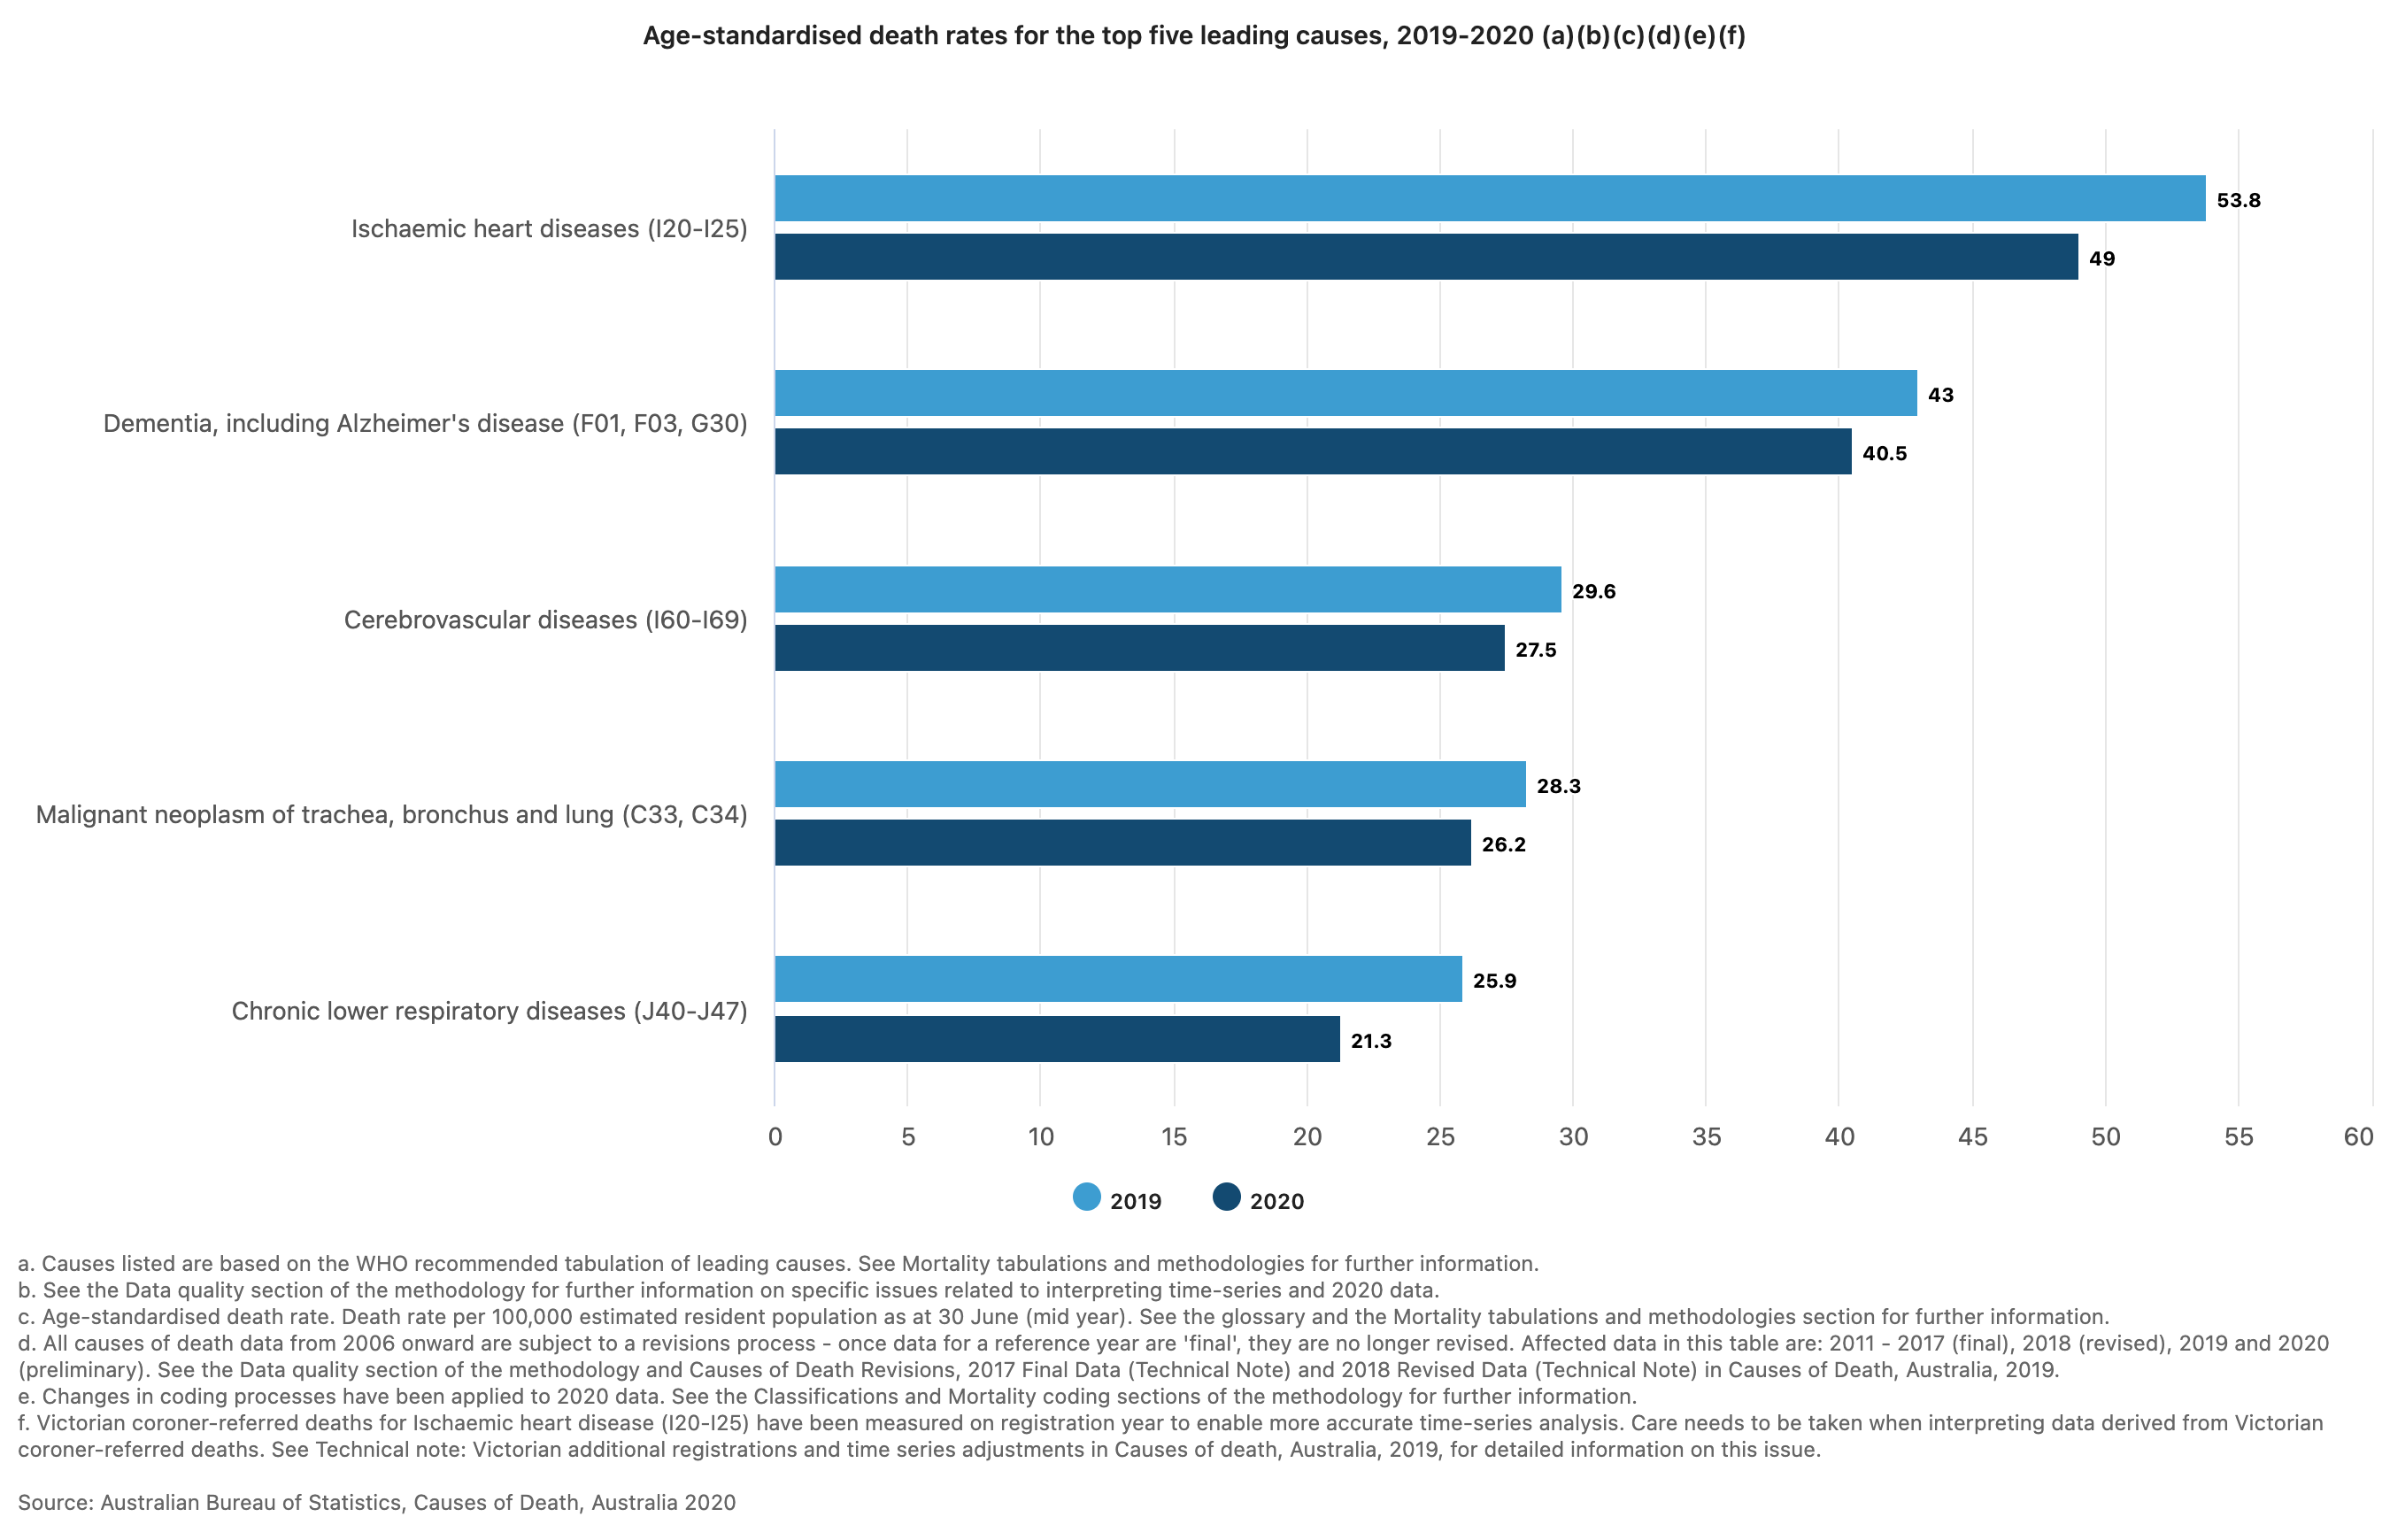
\includegraphics[width=1\textwidth,height=\textheight]{img/mod01/cause-death.png}

}

\caption{\label{fig-1-1}Age-standardised death rates for the top five
leading causes, 2019-2020}

\end{figure}

\hypertarget{inferential-statistics}{%
\subsection{Inferential statistics}\label{inferential-statistics}}

Inferential statistics use data collected from a sample of the
population, to make conclusions (inferences) about the whole population
(that the sample was drawn from).

The following example is about a sample of prisoners, from the National
Prisoner Health Data Collection (NPHDC). The NPHDC is the main source of
national data about the health of prisoners in Australia. It gathers
information over a 2-week period from prison entrants, dischargees,
prisoners visiting the prison health clinic, and prisoners taking
prescribed medication.

We have information about the population of prisoners, given as the
number of prisoners in Australia's prisons from the
\href{http://www.abs.gov.au/ausstats/abs@.nsf/Lookup/by\%20Subject/4517.0~2015~Main\%20Features~Prisoner\%20characteristics,\%20Australia~28}{ABS
website}:

\begin{quote}
At 30 June 2015: There were 36,134 prisoners in Australian prisons, an
increase of 7\% (2,345 prisoners) from 30 June 2014.
\end{quote}

Characteristics (sex, age group and Indigenous status) of the sample of
prisoners from the NPHDC are given in the following table. We can use
this information to make inferences about the whole population of
prisoners that the sample was drawn from.

\begin{figure}[H]

{\centering 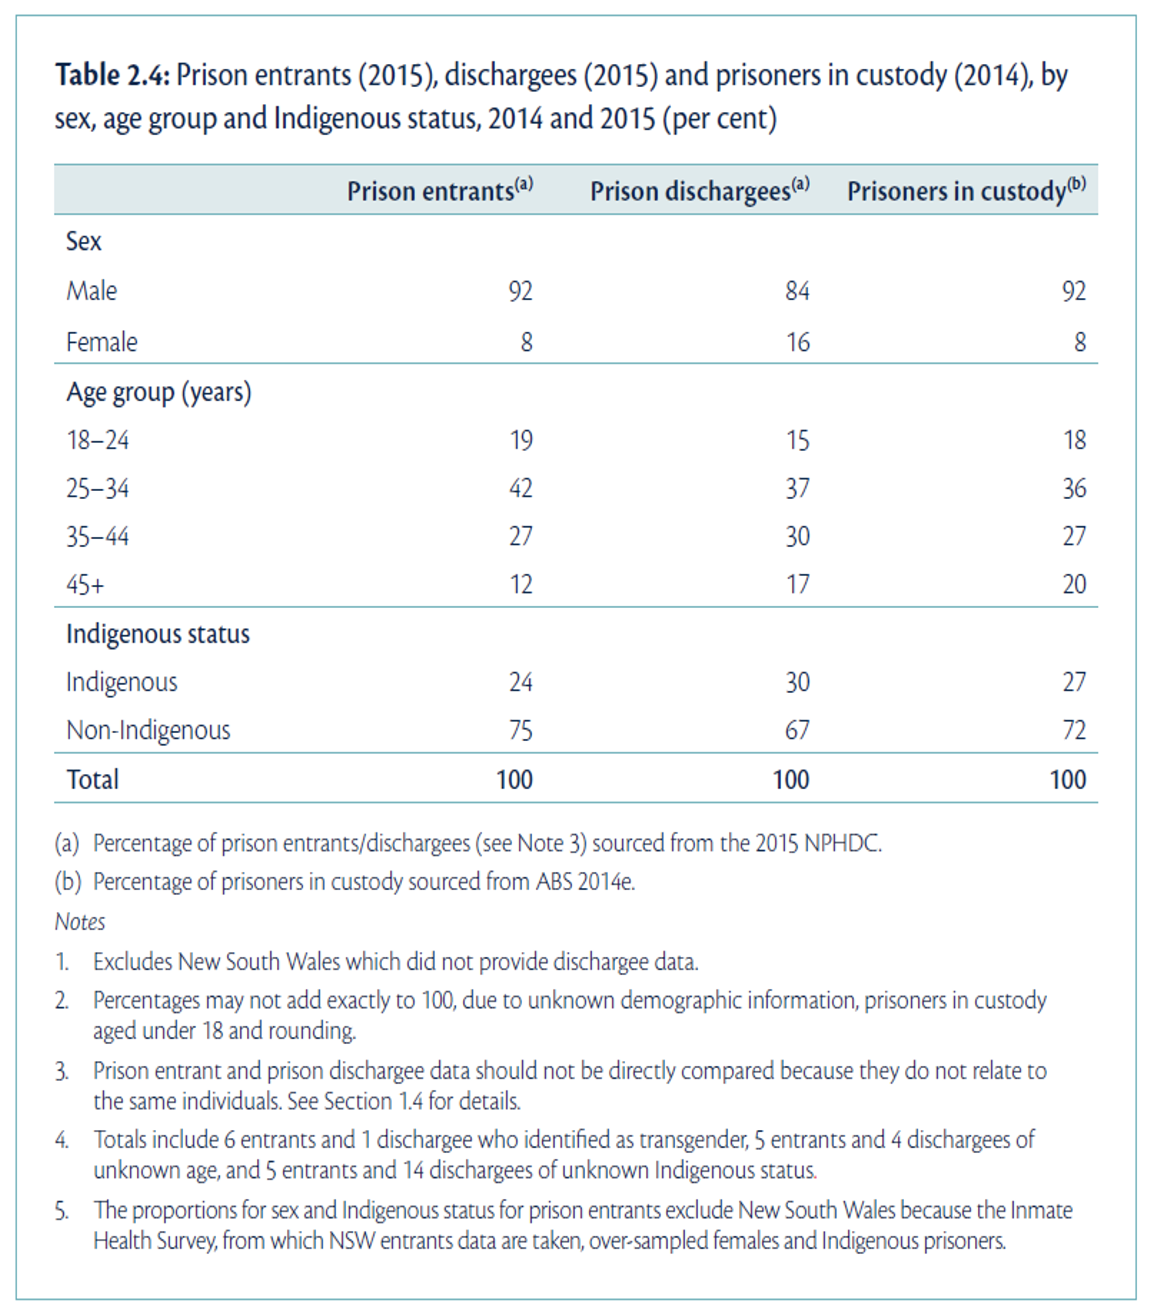
\includegraphics[width=0.66\textwidth,height=\textheight]{img/mod01/prisoner-health.png}

}

\caption{\label{fig-1-2}Characteristics of the sample of prisoners from
the NPHDC}

\end{figure}

\hypertarget{what-are-data}{%
\section{What are data?}\label{what-are-data}}

According to the Australian Bureau of Statistics, ``data are
measurements or observations that are collected as a source of
information''.\footnote{https://www.abs.gov.au/statistics/understanding-statistics/statistical-terms-and-concepts/data}
Note that technically, the word \emph{data} is a plural noun. This may
sound a little odd, but it means that we say ``data are \ldots{}'' when
discussing a set of measurements.

Other definitions that we use in this course are:

\begin{itemize}
\tightlist
\item
  \textbf{observation}, (or \textbf{record}, or \textbf{unit record}):
  one individual in the population being studied
\item
  \textbf{variable}: a characteristic of an individual being measured.
  For example, height, weight, eye colour, income, country of birth are
  all types of variables.
\item
  \textbf{dataset}: the complete collection of all observations
\end{itemize}

\hypertarget{types-of-varaibles}{%
\subsection{Types of varaibles}\label{types-of-varaibles}}

We can categorise variables into two main types: numeric or categorical.

\textbf{Numerical variables} (also called quantitative variables)
comprise data that must be represented by a number, which can be either
measured or counted.

\textbf{Continuous} variables can take any value within a defined range.

For example, age, height, weight or blood pressure, are continuous
variables because we can make any divisions we want on them, and they
can be measured as small as the instrument allows. As an illustration,
if two people have the same blood pressure measured to the nearest
millimetre of mercury, we may get a difference between them if the blood
pressure is measured to the nearest tenth of millimetre. If they are
still the same (to the nearest tenth of a millimetre), we can measure
them with even finer gradations until we can see a difference.

\textbf{Discrete} variables can only take one of a distinct set of
values (usually whole numbers). For discrete variables, observations are
based on a quantity where both ordering and magnitude are important,
such that numbers represent actual measurable quantities rather than
mere labels.

For example, the number of cancer cases in a specified area emerging
over a certain period, the number of motorbike accidents in Sydney, the
number of times a woman has given birth, the number of beds in a
hospital are all discrete variables. Notice that a natural ordering
exists among the data points, that is, a hospital with 100 beds has more
beds than a hospital with 75 beds. Moreover, a difference between 40 and
50 beds is the same as the difference between 80 and 90 beds.

\textbf{Categorical variables} comprise data that describe a `quality'
or `characteristic'. Categorical variables, sometimes called qualitative
variables, do not have measurable numeric values. Categorical variables
can be nominal or ordinal.

A \textbf{nominal} variable consists of unordered categories. For
example, gender, race, ethnic group, religion, eye colour etc. Both the
order and magnitude of a nominal variable are unimportant.

If a nominal variable takes on one of two distinct categories, such as
black or white then it is called a \textbf{binary} or dichotomous
variable. Other examples would be smoker or non-smoker; exposed to
arsenic or not exposed.

A nominal variable can also have more than two categories, such as blood
group, with categories of: Group A, Group B, Group AB and Group O.

\textbf{Ordinal} varaibles consist of ordered categories where
differences between categories are important, such as socioeconomic
status (low, medium, high) or student evaluation rating could be
classified according to their level of satisfaction: (highly satisfied,
satisfied and unsatisfied). Here a natural order exists among the
categories.

Note that categorical variables are often stored in data sets using
numbers to represent categories. However, this is for convenience only,
and these variable must not be analysed as if they were numeric
variables.

\hypertarget{presenting-data}{%
\section{Presenting data}\label{presenting-data}}

We will now look at ways to summarise and present data. The choice of
presentation will depend on the type of variable being summarised. We
will use the dataset based on a study into primary biliary cholangitis
(PBC) from the Introduction to Stata or Introduction to R exercise to
demonstrate the appropriate ways to summarise and present data.

\hypertarget{summarising-a-single-categorical-variable-numerically}{%
\subsection{Summarising a single categorical variable
numerically}\label{summarising-a-single-categorical-variable-numerically}}

Categorical data are best summarised using a frequency table, where each
category is summarised by its frequency: the count of the number of
individuals in each category. The \textbf{relative frequency} (the
frequency expressed as a proportion or percentage of the total
frequency) is usually included give further insight.

\hypertarget{tbl-1-sex}{}
 
  \providecommand{\huxb}[2]{\arrayrulecolor[RGB]{#1}\global\arrayrulewidth=#2pt}
  \providecommand{\huxvb}[2]{\color[RGB]{#1}\vrule width #2pt}
  \providecommand{\huxtpad}[1]{\rule{0pt}{#1}}
  \providecommand{\huxbpad}[1]{\rule[-#1]{0pt}{#1}}

\begin{table}[ht]
\caption{\label{tbl-1-sex}Sex of participants in PBC study }\tabularnewline

\begin{centerbox}
\begin{threeparttable}
 
\setlength{\tabcolsep}{0pt}
\begin{tabularx}{0.8\textwidth}{p{0.266666666666667\textwidth} p{0.266666666666667\textwidth} p{0.266666666666667\textwidth}}


\hhline{>{\huxb{0, 0, 0}{0.4}}->{\huxb{0, 0, 0}{0.4}}->{\huxb{0, 0, 0}{0.4}}-}
\arrayrulecolor{black}

\multicolumn{1}{!{\huxvb{0, 0, 0}{0}}p{0.266666666666667\textwidth}!{\huxvb{0, 0, 0}{0}}}{\hspace{0pt}\parbox[b]{0.266666666666667\textwidth-0pt-6pt}{\huxtpad{6pt + 1em}\raggedright \textbf{Sex}\huxbpad{6pt}}} &
\multicolumn{1}{p{0.266666666666667\textwidth}!{\huxvb{0, 0, 0}{0}}}{\hspace{6pt}\parbox[b]{0.266666666666667\textwidth-6pt-6pt}{\huxtpad{6pt + 1em}\raggedleft \textbf{Frequency}\huxbpad{6pt}}} &
\multicolumn{1}{p{0.266666666666667\textwidth}!{\huxvb{0, 0, 0}{0}}}{\hspace{6pt}\parbox[b]{0.266666666666667\textwidth-6pt-0pt}{\huxtpad{6pt + 1em}\raggedleft \textbf{Relative frequency (\%)}\huxbpad{6pt}}} \tabularnewline[-0.5pt]


\hhline{>{\huxb{0, 0, 0}{0.4}}->{\huxb{0, 0, 0}{0.4}}->{\huxb{0, 0, 0}{0.4}}-}
\arrayrulecolor{black}

\multicolumn{1}{!{\huxvb{0, 0, 0}{0}}p{0.266666666666667\textwidth}!{\huxvb{0, 0, 0}{0}}}{\hspace{0pt}\parbox[b]{0.266666666666667\textwidth-0pt-6pt}{\huxtpad{6pt + 1em}\raggedright Male\huxbpad{6pt}}} &
\multicolumn{1}{p{0.266666666666667\textwidth}!{\huxvb{0, 0, 0}{0}}}{\hspace{6pt}\parbox[b]{0.266666666666667\textwidth-6pt-6pt}{\huxtpad{6pt + 1em}\raggedleft 44\huxbpad{6pt}}} &
\multicolumn{1}{p{0.266666666666667\textwidth}!{\huxvb{0, 0, 0}{0}}}{\hspace{6pt}\parbox[b]{0.266666666666667\textwidth-6pt-0pt}{\huxtpad{6pt + 1em}\raggedleft 10.5\huxbpad{6pt}}} \tabularnewline[-0.5pt]


\hhline{}
\arrayrulecolor{black}

\multicolumn{1}{!{\huxvb{0, 0, 0}{0}}p{0.266666666666667\textwidth}!{\huxvb{0, 0, 0}{0}}}{\hspace{0pt}\parbox[b]{0.266666666666667\textwidth-0pt-6pt}{\huxtpad{6pt + 1em}\raggedright Female\huxbpad{6pt}}} &
\multicolumn{1}{p{0.266666666666667\textwidth}!{\huxvb{0, 0, 0}{0}}}{\hspace{6pt}\parbox[b]{0.266666666666667\textwidth-6pt-6pt}{\huxtpad{6pt + 1em}\raggedleft 374\huxbpad{6pt}}} &
\multicolumn{1}{p{0.266666666666667\textwidth}!{\huxvb{0, 0, 0}{0}}}{\hspace{6pt}\parbox[b]{0.266666666666667\textwidth-6pt-0pt}{\huxtpad{6pt + 1em}\raggedleft 89.5\huxbpad{6pt}}} \tabularnewline[-0.5pt]


\hhline{>{\huxb{0, 0, 0}{0.4}}->{\huxb{0, 0, 0}{0.4}}->{\huxb{0, 0, 0}{0.4}}-}
\arrayrulecolor{black}
\end{tabularx}
\end{threeparttable}\par\end{centerbox}

\end{table}
 

It is sometimes useful to present the cumulative relative frequency,
which shows the relative frequency of individuals in a certain category
or below (for example, Table~\ref{tbl-1-stage}).

\hypertarget{tbl-1-stage}{}
 
  \providecommand{\huxb}[2]{\arrayrulecolor[RGB]{#1}\global\arrayrulewidth=#2pt}
  \providecommand{\huxvb}[2]{\color[RGB]{#1}\vrule width #2pt}
  \providecommand{\huxtpad}[1]{\rule{0pt}{#1}}
  \providecommand{\huxbpad}[1]{\rule[-#1]{0pt}{#1}}

\begin{table}[ht]
\caption{\label{tbl-1-stage}Stage of disease for participants in PBC study }\tabularnewline

\begin{centerbox}
\begin{threeparttable}
 
\setlength{\tabcolsep}{0pt}
\begin{tabularx}{0.8\textwidth}{p{0.2\textwidth} p{0.2\textwidth} p{0.2\textwidth} p{0.2\textwidth}}


\hhline{>{\huxb{0, 0, 0}{0.4}}->{\huxb{0, 0, 0}{0.4}}->{\huxb{0, 0, 0}{0.4}}->{\huxb{0, 0, 0}{0.4}}-}
\arrayrulecolor{black}

\multicolumn{1}{!{\huxvb{0, 0, 0}{0}}p{0.2\textwidth}!{\huxvb{0, 0, 0}{0}}}{\hspace{0pt}\parbox[b]{0.2\textwidth-0pt-6pt}{\huxtpad{6pt + 1em}\raggedright \textbf{Stage *}\huxbpad{6pt}}} &
\multicolumn{1}{p{0.2\textwidth}!{\huxvb{0, 0, 0}{0}}}{\hspace{6pt}\parbox[b]{0.2\textwidth-6pt-6pt}{\huxtpad{6pt + 1em}\raggedleft \textbf{Frequency}\huxbpad{6pt}}} &
\multicolumn{1}{p{0.2\textwidth}!{\huxvb{0, 0, 0}{0}}}{\hspace{6pt}\parbox[b]{0.2\textwidth-6pt-6pt}{\huxtpad{6pt + 1em}\raggedleft \textbf{Relative frequency (\%)}\huxbpad{6pt}}} &
\multicolumn{1}{p{0.2\textwidth}!{\huxvb{0, 0, 0}{0}}}{\hspace{6pt}\parbox[b]{0.2\textwidth-6pt-0pt}{\huxtpad{6pt + 1em}\raggedleft \textbf{Cumulative relative frequency (\%)}\huxbpad{6pt}}} \tabularnewline[-0.5pt]


\hhline{>{\huxb{0, 0, 0}{0.4}}->{\huxb{0, 0, 0}{0.4}}->{\huxb{0, 0, 0}{0.4}}->{\huxb{0, 0, 0}{0.4}}-}
\arrayrulecolor{black}

\multicolumn{1}{!{\huxvb{0, 0, 0}{0}}p{0.2\textwidth}!{\huxvb{0, 0, 0}{0}}}{\hspace{0pt}\parbox[b]{0.2\textwidth-0pt-6pt}{\huxtpad{6pt + 1em}\raggedright 1\huxbpad{6pt}}} &
\multicolumn{1}{p{0.2\textwidth}!{\huxvb{0, 0, 0}{0}}}{\hspace{6pt}\parbox[b]{0.2\textwidth-6pt-6pt}{\huxtpad{6pt + 1em}\raggedleft 21\huxbpad{6pt}}} &
\multicolumn{1}{p{0.2\textwidth}!{\huxvb{0, 0, 0}{0}}}{\hspace{6pt}\parbox[b]{0.2\textwidth-6pt-6pt}{\huxtpad{6pt + 1em}\raggedleft 5.1\huxbpad{6pt}}} &
\multicolumn{1}{p{0.2\textwidth}!{\huxvb{0, 0, 0}{0}}}{\hspace{6pt}\parbox[b]{0.2\textwidth-6pt-0pt}{\huxtpad{6pt + 1em}\raggedleft 5.1\huxbpad{6pt}}} \tabularnewline[-0.5pt]


\hhline{}
\arrayrulecolor{black}

\multicolumn{1}{!{\huxvb{0, 0, 0}{0}}p{0.2\textwidth}!{\huxvb{0, 0, 0}{0}}}{\hspace{0pt}\parbox[b]{0.2\textwidth-0pt-6pt}{\huxtpad{6pt + 1em}\raggedright 2\huxbpad{6pt}}} &
\multicolumn{1}{p{0.2\textwidth}!{\huxvb{0, 0, 0}{0}}}{\hspace{6pt}\parbox[b]{0.2\textwidth-6pt-6pt}{\huxtpad{6pt + 1em}\raggedleft 92\huxbpad{6pt}}} &
\multicolumn{1}{p{0.2\textwidth}!{\huxvb{0, 0, 0}{0}}}{\hspace{6pt}\parbox[b]{0.2\textwidth-6pt-6pt}{\huxtpad{6pt + 1em}\raggedleft 22.3\huxbpad{6pt}}} &
\multicolumn{1}{p{0.2\textwidth}!{\huxvb{0, 0, 0}{0}}}{\hspace{6pt}\parbox[b]{0.2\textwidth-6pt-0pt}{\huxtpad{6pt + 1em}\raggedleft 27.4\huxbpad{6pt}}} \tabularnewline[-0.5pt]


\hhline{}
\arrayrulecolor{black}

\multicolumn{1}{!{\huxvb{0, 0, 0}{0}}p{0.2\textwidth}!{\huxvb{0, 0, 0}{0}}}{\hspace{0pt}\parbox[b]{0.2\textwidth-0pt-6pt}{\huxtpad{6pt + 1em}\raggedright 3\huxbpad{6pt}}} &
\multicolumn{1}{p{0.2\textwidth}!{\huxvb{0, 0, 0}{0}}}{\hspace{6pt}\parbox[b]{0.2\textwidth-6pt-6pt}{\huxtpad{6pt + 1em}\raggedleft 155\huxbpad{6pt}}} &
\multicolumn{1}{p{0.2\textwidth}!{\huxvb{0, 0, 0}{0}}}{\hspace{6pt}\parbox[b]{0.2\textwidth-6pt-6pt}{\huxtpad{6pt + 1em}\raggedleft 37.6\huxbpad{6pt}}} &
\multicolumn{1}{p{0.2\textwidth}!{\huxvb{0, 0, 0}{0}}}{\hspace{6pt}\parbox[b]{0.2\textwidth-6pt-0pt}{\huxtpad{6pt + 1em}\raggedleft 65.0\huxbpad{6pt}}} \tabularnewline[-0.5pt]


\hhline{}
\arrayrulecolor{black}

\multicolumn{1}{!{\huxvb{0, 0, 0}{0}}p{0.2\textwidth}!{\huxvb{0, 0, 0}{0}}}{\hspace{0pt}\parbox[b]{0.2\textwidth-0pt-6pt}{\huxtpad{6pt + 1em}\raggedright 4\huxbpad{6pt}}} &
\multicolumn{1}{p{0.2\textwidth}!{\huxvb{0, 0, 0}{0}}}{\hspace{6pt}\parbox[b]{0.2\textwidth-6pt-6pt}{\huxtpad{6pt + 1em}\raggedleft 144\huxbpad{6pt}}} &
\multicolumn{1}{p{0.2\textwidth}!{\huxvb{0, 0, 0}{0}}}{\hspace{6pt}\parbox[b]{0.2\textwidth-6pt-6pt}{\huxtpad{6pt + 1em}\raggedleft 35.0\huxbpad{6pt}}} &
\multicolumn{1}{p{0.2\textwidth}!{\huxvb{0, 0, 0}{0}}}{\hspace{6pt}\parbox[b]{0.2\textwidth-6pt-0pt}{\huxtpad{6pt + 1em}\raggedleft 100.0\huxbpad{6pt}}} \tabularnewline[-0.5pt]


\hhline{>{\huxb{0, 0, 0}{0.8}}->{\huxb{0, 0, 0}{0.8}}->{\huxb{0, 0, 0}{0.8}}->{\huxb{0, 0, 0}{0.8}}-}
\arrayrulecolor{black}

\multicolumn{4}{!{\huxvb{0, 0, 0}{0}}p{0.8\textwidth+6\tabcolsep}!{\huxvb{0, 0, 0}{0}}}{\hspace{6pt}\parbox[b]{0.8\textwidth+6\tabcolsep-6pt-6pt}{\huxtpad{6pt + 1em}\raggedright * Disease stage was missing for 6 participants\huxbpad{6pt}}} \tabularnewline[-0.5pt]


\hhline{}
\arrayrulecolor{black}
\end{tabularx}
\end{threeparttable}\par\end{centerbox}

\end{table}
 

From Table~\ref{tbl-1-stage}, we can see that 65.0\% of participants had
Stage 3 disease or lower.

\hypertarget{summarising-a-single-categorical-variable-graphically}{%
\subsection{Summarising a single categorical variable
graphically}\label{summarising-a-single-categorical-variable-graphically}}

A categorical variable is best summarised graphically using a
\textbf{bar chart}. For example, we can present the distribution of
Stage of Disease graphically using a bar graph (Figure~\ref{fig-bar-1}).
Bar graphs, which are suitable for plotting discrete or categorical
variables, are defined by the fact that the bars do not touch.

\begin{figure}[H]

{\centering 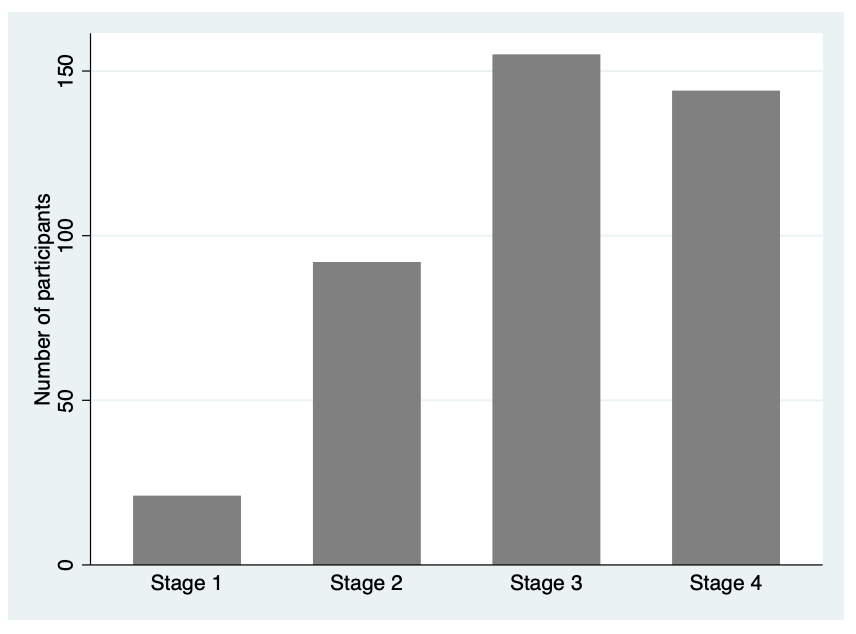
\includegraphics[width=0.75\textwidth,height=\textheight]{img/mod01/pbc-bar.png}

}

\caption{\label{fig-bar-1}Bar graph of stage of disease from PBC study}

\end{figure}

Pie charts can be an alternative way to summarise a categorical variable
graphically, however their use is not recommended for the following
reasons:

\begin{itemize}
\tightlist
\item
  Not ideal when there are many categories to compare
\item
  The use of percentages is not appropriate when the sample size is
  small
\item
  Can be misleading by using different size pies, different rotations
  and different colours to draw attention to specific groups
\item
  3D and exploding bar charts further distort the effect of perspective
  and may confuse the reader
\end{itemize}

Pie charts will not be discussed further in this course.

\hypertarget{summarising-a-single-continuous-variable-numerically}{%
\subsection{Summarising a single continuous variable
numerically}\label{summarising-a-single-continuous-variable-numerically}}

When summarising continuous data numerically, there are two things we
want to know:

\begin{enumerate}
\def\labelenumi{\arabic{enumi}.}
\tightlist
\item
  What is the average value? And,
\item
  How variable (or spread out) are the data?
\end{enumerate}

We will use a sample of 35 ages (in whole years) to illustrate how to
calculate the average value and measures of variability:

59 41 44 43 31 47 53 59 35 60 54 61 67 52 43 46 39 69 50 64 57 39 54 50
51 31 48 49 70 44 60 51 37 53 34

\hypertarget{measures-of-central-tendency}{%
\subsubsection{Measures of central
tendency}\label{measures-of-central-tendency}}

\hypertarget{mean}{%
\subsubsection{Mean}\label{mean}}

The most commonly used measure of the central tendency of the data is
the mean, calculated as:

\[\bar{x} = \frac{\sum x}{n}\]

From the age example: \(\bar{x}\) = 1745/35 = 49.9. Thus, the mean age
of this sample is 49.9 years.

\hypertarget{median}{%
\subsubsection{Median}\label{median}}

Other measures of central tendency include the median and mode. The
median is the middle value of the data, the value at which half of the
measurements lie above it and half of the measurements lie below it.

To estimate the median, the data are ordered from the lowest to highest
values, and the middle value is used. If the middle value is between two
data points (if there are an even number of observations), the median is
an average of the two values.

Using our example, we could rank the ages from smallest to largest, and
locate the middle value (which has been bolded):

31 31 34 35 37 39 39 41 43 43 44 44 46 47 48 49 50 \textbf{50} 51 51 52
53 53 54 54 57 59 59 60 60 61 64 67 69 70

Here, the median is estimated as 50 years.

Note that, in practice, the median is usually calculated by software
automatically, and there is no need to rank our data.

\hypertarget{describing-the-spread-of-the-data}{%
\subsubsection{Describing the spread of the
data}\label{describing-the-spread-of-the-data}}

In addition to measuring the centre of the data, we also need an
estimate of the variability, or spread, of the data points.

\hypertarget{range}{%
\subsubsection{Range}\label{range}}

The absolute measure of the spread of the data is the range, that is the
difference between the highest and lowest values in the dataset.

Range = highest data value -- lowest data value

Using the age example, Range = 70 - 31 = 39 years.

The range is most usefully reported as the actual lowest and highest
values e.g.~Range: 31 to 70 years.

The range is not always ideal as it only describes the extreme values,
without considering how the bulk of the data is distributed between
them.

\hypertarget{variance-and-standard-deviation}{%
\subsubsection{Variance and standard
deviation}\label{variance-and-standard-deviation}}

More useful statistics to describe the spread of the data around a mean
value are the variance and standard deviation. These measures of
variability depend on the difference between individual observations and
the mean value (deviations). If all values are equal to the mean there
would be no variability at all, all deviations would be zero; conversely
large deviations indicate greater variability.

One way of combining deviations in a single measure is to first square
the deviations and then average the squares. Squaring is done because we
are equally interested in negative deviations and positive deviations;
if we averaged without squaring, negative and positive deviations would
`cancel out'. This measure is called the variance of the set of
observations. It is `the average squared deviation from the mean'.
Because the variance is in `square' units and not in the units of the
measurement, a second measure is derived by taking the square root of
the variance. This is the standard deviation (SD), and is the most
commonly used measure of variability in practice, as it is a more
intuitive interpretation since it is in the same units as the units of
measurement.

The formula for the variance of a sample (\(s^2\)) is:

\[ s^2 = \frac{\sum(x - \bar{x})^2}{n-1} \]

Note that the deviations are first squared before they are summed to
remove the negative values; once summed they are divided by the sample
size minus 1.

The sample standard deviation is the square root of the of the sample
variance:

\[s = \sqrt{s^2}\] For the age example, we would calculate the sample
variance using statistical software. The sample standard deviation is
estimated as: \(s = 10.47 \text{ years}\).

Characteristics of the standard deviation:

\begin{itemize}
\tightlist
\item
  It is affected by every measurement
\item
  It is in the same units as the measurements
\item
  It can be converted to measures of precision (standard error and 95\%
  confidence intervals) (Module 3)
\end{itemize}

\hypertarget{interquartile-range}{%
\subsubsection{Interquartile range}\label{interquartile-range}}

The inter-quartile range (IQR) describes the range of measurements in
the central 50\% of values lie. This is estimated by calculating the
values that cut the data at the bottom 25\% and top 25\%. The IQR is the
preferred measure of spread when the median has been used to describe
central tendency.

In the age example, the IQR is estimated as 43 to 59 years. Note that R
and Stata use slightly different methods to calculate the interquartile
range (Stata IQR: 43 to 59 years; R IQR: 43 to 58 years). This
difference is not practically important, and either range would be
considered correct.

\hypertarget{population-values-mean-variance-and-standard-deviation}{%
\subsubsection{Population values: mean, variance and standard
deviation}\label{population-values-mean-variance-and-standard-deviation}}

The examples above show how the sample mean, range, variance and
standard deviation are calculated from the sample of ages from 35
people. If we had information on the age of the \emph{entire} population
that the sample was drawn from, we could calculate all the summary
statistics described above (for the sample) for the population.

The equation for calculating the population mean is the same as that of
sample mean, though now we denote the population mean as \(\mu\):

\[ \mu = \frac{\sum{x}}{N} \]

Where \(\sum{x}\) represents the sum of the values in the population,
and \(N\) represents the total number of measurements in the population.

To calculate the population variance (\(\sigma^2\)) and standard
deviation(\(\sigma\)), we use a slightly modified version of the
equation for \(s^2\):

\[ \sigma^2 = \frac{\sum(x - \mu)^2}{N} \]

with a population standard deviation of: \(\sigma = \sqrt{\sigma^2}\).

In practice, we rarely have the information for the entire population to
be able to calculate the population mean and standard deviation.
Theoretically, however, these statistics are important for two main
purposes:

\begin{enumerate}
\def\labelenumi{\arabic{enumi}.}
\tightlist
\item
  the characteristics of the normal distribution (the most important
  probability distribution discussed in later modules) are defined by
  the population mean and standard deviation;
\item
  while calculating sample sizes (discussed in later modules) we need
  information about the population standard deviation, which is usually
  obtained from the existing literature.
\end{enumerate}

\hypertarget{summarising-a-single-continuous-variable-graphically}{%
\subsection{Summarising a single continuous variable
graphically}\label{summarising-a-single-continuous-variable-graphically}}

As well as calculating measures of central tendency and spread to
describe the characteristics of the data, a graphical plot is very
helpful to better understand the characteristics and distribution of the
measurements obtained. \emph{Histograms} and \emph{box plots} are
excellent ways to graphically display continuous data.

\hypertarget{frequency-histograms}{%
\subsubsection{Frequency histograms}\label{frequency-histograms}}

A histogram that plots the frequency of the grouped observations is
called a frequency histogram. Some features of a frequency histogram:

\begin{itemize}
\tightlist
\item
  The area under each rectangle is proportional to the frequency
\item
  The rectangles are drawn without gaps between them (unlike a bar
  graph)
\item
  The data are `binned' into discrete intervals (of (usually of equal
  width)
\end{itemize}

If the rectangles are symmetrically distributed about the middle of the
histogram, we say that the data are symmetric, and the mean and median
will be approximately equal.

If the histogram has a longer tail to the right, then the data are said
to be positively skewed (or skewed to the right), and the mean will be
greater than the median.

If the histogram has an extended tail to the left, then the data are
negatively skewed (or skewed to the left) and the mean will be smaller
than the median.

\begin{quote}
The skewness of a distribution is defined by the location of the longer
tail, not the location of the peak of the data.
\end{quote}

Figure~\ref{fig-hist-1} presents two histograms from the PBC data from
the Introduction to Stata exercise: for age and serum bilirubin. We can
see that the distribution for age is roughly symmetric, while the
distribution for serum bilirubin is highly positively skewed (or skewed
to the right).

\begin{figure}

{\centering 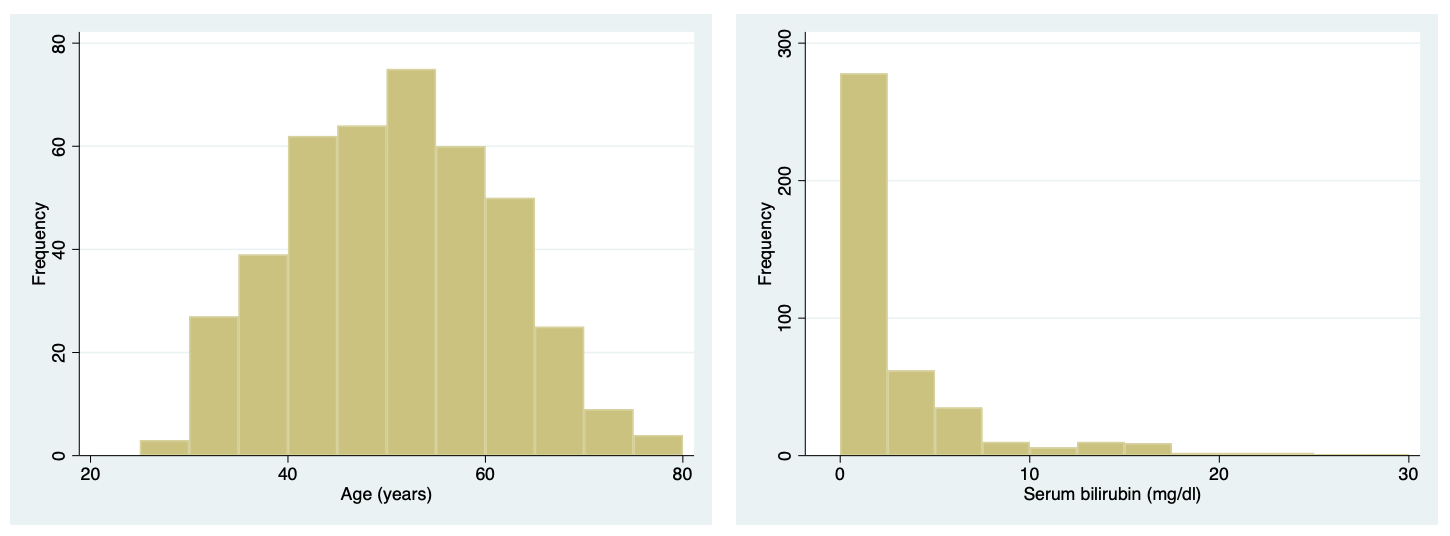
\includegraphics[width=1\textwidth,height=\textheight]{img/mod01/hist-symmetric-skewed.png}

}

\caption{\label{fig-hist-1}Histogram of age (left) and serum bilirubin
(right) from PBC study data}

\end{figure}

A slight variation on the frequency histogram is the \textbf{density
histogram}, which plots the density on the y-axis. The density is a
technical term, which is similar to the relative frequency, but is
scaled so that the sum of the area of the bars is equal to 1.

Both the frequency and density histograms are useful for understanding
how the data is distributed across the range of values. Taller bars
indicate regions where the data is more densely concentrated, while
shorter bars represent areas with fewer data points.

\hypertarget{boxplots}{%
\subsubsection{Boxplots}\label{boxplots}}

Another useful way to inspect the distribution of data is by using a box
plot. In a box plot:

\begin{itemize}
\tightlist
\item
  the line across the box shows the median value
\item
  the limits of the box show the 25-75\% range (i.e.~the inter-quartile
  range (IQR) where the middle 50\% of the data lie)
\item
  the bars (or whiskers) indicate the most extreme values (highest and
  lowest) that fall within 1.5 times the interquartile range from each
  end of the box

  \begin{itemize}
  \tightlist
  \item
    the upper whisker is the highest value falling within 75th
    percentile plus 1.5 × IQR
  \item
    the lower whisker is the lowest value falling within 25th percentile
    minus 1.5 × IQR
  \end{itemize}
\item
  any values in the dataset lying outside the whiskers are plotted
  individually.
\end{itemize}

If the data are symmetric, the line across the box (the median value)
will be in the centre of the box, and the tails will be roughly equal.

Figure~\ref{fig-box-1} presents two boxplots from the PBC data: for age
and serum bilirubin. We can see that the boxplot for age has roughly
equal tails, and the median (the horizontal line) lies roughly in the
middle of the interquartile range (the shaded box). It would be
reasonable to assume that age follows a symmetric distribution from this
plot. The boxplot for serum bilirubin shows a much longer upper tail,
and a median much closer to the bottom of the shaded box than the
middle. The boxplot also shows a number of points above the 75th
percentile plus 1.5 × IQR. As the upper tail is longer than the lower
tail, this distribution is positively skewed.

\begin{figure}

{\centering 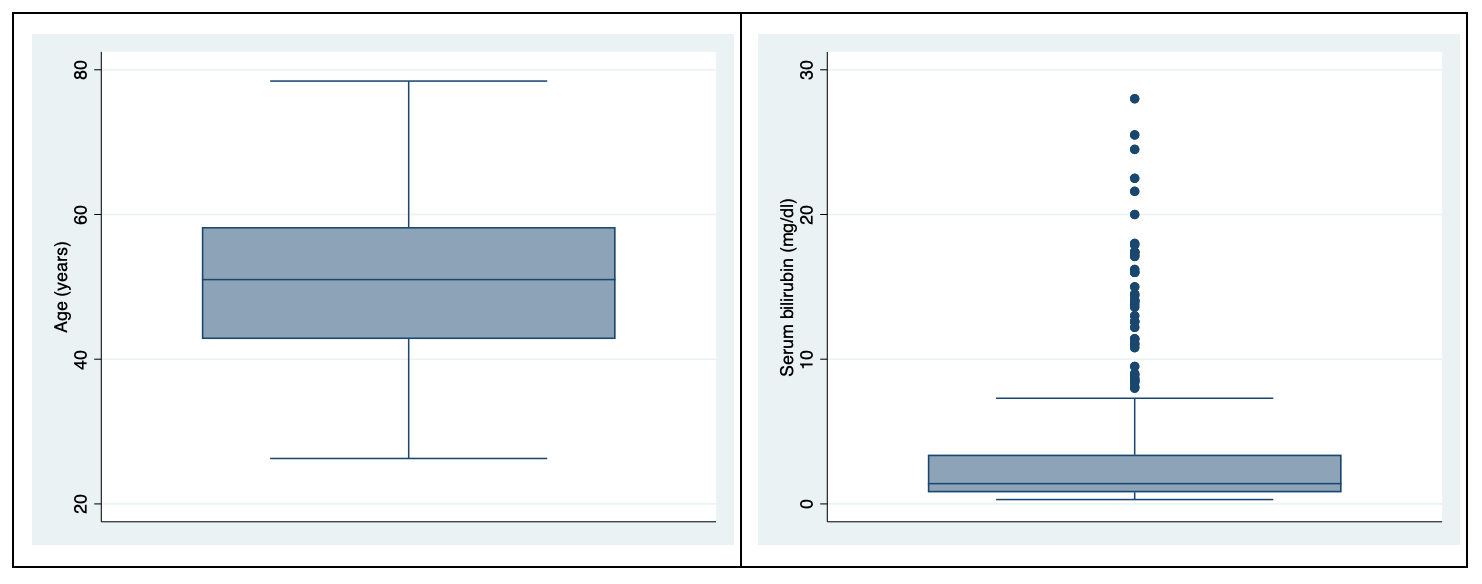
\includegraphics[width=1\textwidth,height=\textheight]{img/mod01/boxp-symmetric-skewed.png}

}

\caption{\label{fig-box-1}Box plot of age (left) and serum bilirubin
(right) from PBC study data}

\end{figure}

\hypertarget{summarising-two-categorical-variables-numerically}{%
\subsection{Summarising two categorical variables
numerically}\label{summarising-two-categorical-variables-numerically}}

So far, we have discussed one-way frequency tables, that is, tables that
summarise one variable. We can summarise more than two categorical
variables in a table -- called a cross tabulation, or a two-way
(summarising two variables) table.

Using our PBC data, we can summarise the two categorical variables: sex
and stage of disease. The two-way table of frequencies is shown in
Table~\ref{tbl-1-sex-stage-freq}.

\hypertarget{tbl-1-sex-stage-freq}{}
 
  \providecommand{\huxb}[2]{\arrayrulecolor[RGB]{#1}\global\arrayrulewidth=#2pt}
  \providecommand{\huxvb}[2]{\color[RGB]{#1}\vrule width #2pt}
  \providecommand{\huxtpad}[1]{\rule{0pt}{#1}}
  \providecommand{\huxbpad}[1]{\rule[-#1]{0pt}{#1}}

\begin{table}[ht]
\caption{\label{tbl-1-sex-stage-freq}Frequency of participants by sex and stage of disease* }\tabularnewline

\begin{centerbox}
\begin{threeparttable}
 
\setlength{\tabcolsep}{0pt}
\begin{tabularx}{0.9\textwidth}{p{0.15\textwidth} p{0.15\textwidth} p{0.15\textwidth} p{0.15\textwidth} p{0.15\textwidth} p{0.15\textwidth}}


\hhline{>{\huxb{0, 0, 0}{0.4}}->{\huxb{0, 0, 0}{0.4}}->{\huxb{0, 0, 0}{0.4}}->{\huxb{0, 0, 0}{0.4}}->{\huxb{0, 0, 0}{0.4}}->{\huxb{0, 0, 0}{0.4}}-}
\arrayrulecolor{black}

\multicolumn{1}{!{\huxvb{0, 0, 0}{0}}p{0.15\textwidth}!{\huxvb{0, 0, 0}{0}}}{\hspace{0pt}\parbox[b]{0.15\textwidth-0pt-6pt}{\huxtpad{6pt + 1em}\raggedright \textbf{
}\huxbpad{6pt}}} &
\multicolumn{4}{p{0.6\textwidth+6\tabcolsep}!{\huxvb{0, 0, 0}{0}}}{\hspace{6pt}\parbox[b]{0.6\textwidth+6\tabcolsep-6pt-6pt}{\huxtpad{6pt + 1em}\centering \textbf{Stage
}\huxbpad{6pt}}} &
\multicolumn{1}{p{0.15\textwidth}!{\huxvb{0, 0, 0}{0}}}{\hspace{6pt}\parbox[b]{0.15\textwidth-6pt-0pt}{\huxtpad{6pt + 1em}\centering \textbf{
}\huxbpad{6pt}}} \tabularnewline[-0.5pt]


\hhline{}
\arrayrulecolor{black}

\multicolumn{1}{!{\huxvb{0, 0, 0}{0}}p{0.15\textwidth}!{\huxvb{0, 0, 0}{0}}}{\hspace{0pt}\parbox[b]{0.15\textwidth-0pt-6pt}{\huxtpad{6pt + 1em}\raggedright \textbf{
}\huxbpad{6pt}}} &
\multicolumn{1}{p{0.15\textwidth}!{\huxvb{0, 0, 0}{0}}}{\hspace{6pt}\parbox[b]{0.15\textwidth-6pt-6pt}{\huxtpad{6pt + 1em}\centering \textbf{1
}\huxbpad{6pt}}} &
\multicolumn{1}{p{0.15\textwidth}!{\huxvb{0, 0, 0}{0}}}{\hspace{6pt}\parbox[b]{0.15\textwidth-6pt-6pt}{\huxtpad{6pt + 1em}\centering \textbf{2
}\huxbpad{6pt}}} &
\multicolumn{1}{p{0.15\textwidth}!{\huxvb{0, 0, 0}{0}}}{\hspace{6pt}\parbox[b]{0.15\textwidth-6pt-6pt}{\huxtpad{6pt + 1em}\centering \textbf{3
}\huxbpad{6pt}}} &
\multicolumn{1}{p{0.15\textwidth}!{\huxvb{0, 0, 0}{0}}}{\hspace{6pt}\parbox[b]{0.15\textwidth-6pt-6pt}{\huxtpad{6pt + 1em}\centering \textbf{4
}\huxbpad{6pt}}} &
\multicolumn{1}{p{0.15\textwidth}!{\huxvb{0, 0, 0}{0}}}{\hspace{6pt}\parbox[b]{0.15\textwidth-6pt-0pt}{\huxtpad{6pt + 1em}\centering \textbf{Total
}\huxbpad{6pt}}} \tabularnewline[-0.5pt]


\hhline{>{\huxb{0, 0, 0}{0.4}}->{\huxb{0, 0, 0}{0.4}}->{\huxb{0, 0, 0}{0.4}}->{\huxb{0, 0, 0}{0.4}}->{\huxb{0, 0, 0}{0.4}}->{\huxb{0, 0, 0}{0.4}}-}
\arrayrulecolor{black}

\multicolumn{1}{!{\huxvb{0, 0, 0}{0}}p{0.15\textwidth}!{\huxvb{0, 0, 0}{0}}}{\hspace{0pt}\parbox[b]{0.15\textwidth-0pt-6pt}{\huxtpad{6pt + 1em}\raggedright Sex\huxbpad{6pt}}} &
\multicolumn{1}{p{0.15\textwidth}!{\huxvb{0, 0, 0}{0}}}{\hspace{6pt}\parbox[b]{0.15\textwidth-6pt-6pt}{\huxtpad{6pt + 1em}\centering \huxbpad{6pt}}} &
\multicolumn{1}{p{0.15\textwidth}!{\huxvb{0, 0, 0}{0}}}{\hspace{6pt}\parbox[b]{0.15\textwidth-6pt-6pt}{\huxtpad{6pt + 1em}\centering \huxbpad{6pt}}} &
\multicolumn{1}{p{0.15\textwidth}!{\huxvb{0, 0, 0}{0}}}{\hspace{6pt}\parbox[b]{0.15\textwidth-6pt-6pt}{\huxtpad{6pt + 1em}\centering \huxbpad{6pt}}} &
\multicolumn{1}{p{0.15\textwidth}!{\huxvb{0, 0, 0}{0}}}{\hspace{6pt}\parbox[b]{0.15\textwidth-6pt-6pt}{\huxtpad{6pt + 1em}\centering \huxbpad{6pt}}} &
\multicolumn{1}{p{0.15\textwidth}!{\huxvb{0, 0, 0}{0}}}{\hspace{6pt}\parbox[b]{0.15\textwidth-6pt-0pt}{\huxtpad{6pt + 1em}\centering \huxbpad{6pt}}} \tabularnewline[-0.5pt]


\hhline{}
\arrayrulecolor{black}

\multicolumn{1}{!{\huxvb{0, 0, 0}{0}}p{0.15\textwidth}!{\huxvb{0, 0, 0}{0}}}{\hspace{0pt}\parbox[b]{0.15\textwidth-0pt-6pt}{\huxtpad{6pt + 1em}\raggedright Male\huxbpad{6pt}}} &
\multicolumn{1}{p{0.15\textwidth}!{\huxvb{0, 0, 0}{0}}}{\hspace{6pt}\parbox[b]{0.15\textwidth-6pt-6pt}{\huxtpad{6pt + 1em}\centering 3\huxbpad{6pt}}} &
\multicolumn{1}{p{0.15\textwidth}!{\huxvb{0, 0, 0}{0}}}{\hspace{6pt}\parbox[b]{0.15\textwidth-6pt-6pt}{\huxtpad{6pt + 1em}\centering 8\huxbpad{6pt}}} &
\multicolumn{1}{p{0.15\textwidth}!{\huxvb{0, 0, 0}{0}}}{\hspace{6pt}\parbox[b]{0.15\textwidth-6pt-6pt}{\huxtpad{6pt + 1em}\centering 16\huxbpad{6pt}}} &
\multicolumn{1}{p{0.15\textwidth}!{\huxvb{0, 0, 0}{0}}}{\hspace{6pt}\parbox[b]{0.15\textwidth-6pt-6pt}{\huxtpad{6pt + 1em}\centering 17\huxbpad{6pt}}} &
\multicolumn{1}{p{0.15\textwidth}!{\huxvb{0, 0, 0}{0}}}{\hspace{6pt}\parbox[b]{0.15\textwidth-6pt-0pt}{\huxtpad{6pt + 1em}\centering 44\huxbpad{6pt}}} \tabularnewline[-0.5pt]


\hhline{}
\arrayrulecolor{black}

\multicolumn{1}{!{\huxvb{0, 0, 0}{0}}p{0.15\textwidth}!{\huxvb{0, 0, 0}{0}}}{\hspace{0pt}\parbox[b]{0.15\textwidth-0pt-6pt}{\huxtpad{6pt + 1em}\raggedright Female\huxbpad{6pt}}} &
\multicolumn{1}{p{0.15\textwidth}!{\huxvb{0, 0, 0}{0}}}{\hspace{6pt}\parbox[b]{0.15\textwidth-6pt-6pt}{\huxtpad{6pt + 1em}\centering 18\huxbpad{6pt}}} &
\multicolumn{1}{p{0.15\textwidth}!{\huxvb{0, 0, 0}{0}}}{\hspace{6pt}\parbox[b]{0.15\textwidth-6pt-6pt}{\huxtpad{6pt + 1em}\centering 84\huxbpad{6pt}}} &
\multicolumn{1}{p{0.15\textwidth}!{\huxvb{0, 0, 0}{0}}}{\hspace{6pt}\parbox[b]{0.15\textwidth-6pt-6pt}{\huxtpad{6pt + 1em}\centering 139\huxbpad{6pt}}} &
\multicolumn{1}{p{0.15\textwidth}!{\huxvb{0, 0, 0}{0}}}{\hspace{6pt}\parbox[b]{0.15\textwidth-6pt-6pt}{\huxtpad{6pt + 1em}\centering 127\huxbpad{6pt}}} &
\multicolumn{1}{p{0.15\textwidth}!{\huxvb{0, 0, 0}{0}}}{\hspace{6pt}\parbox[b]{0.15\textwidth-6pt-0pt}{\huxtpad{6pt + 1em}\centering 368\huxbpad{6pt}}} \tabularnewline[-0.5pt]


\hhline{}
\arrayrulecolor{black}

\multicolumn{1}{!{\huxvb{0, 0, 0}{0}}p{0.15\textwidth}!{\huxvb{0, 0, 0}{0}}}{\hspace{0pt}\parbox[b]{0.15\textwidth-0pt-6pt}{\huxtpad{6pt + 1em}\raggedright Total\huxbpad{6pt}}} &
\multicolumn{1}{p{0.15\textwidth}!{\huxvb{0, 0, 0}{0}}}{\hspace{6pt}\parbox[b]{0.15\textwidth-6pt-6pt}{\huxtpad{6pt + 1em}\centering 21\huxbpad{6pt}}} &
\multicolumn{1}{p{0.15\textwidth}!{\huxvb{0, 0, 0}{0}}}{\hspace{6pt}\parbox[b]{0.15\textwidth-6pt-6pt}{\huxtpad{6pt + 1em}\centering 92\huxbpad{6pt}}} &
\multicolumn{1}{p{0.15\textwidth}!{\huxvb{0, 0, 0}{0}}}{\hspace{6pt}\parbox[b]{0.15\textwidth-6pt-6pt}{\huxtpad{6pt + 1em}\centering 155\huxbpad{6pt}}} &
\multicolumn{1}{p{0.15\textwidth}!{\huxvb{0, 0, 0}{0}}}{\hspace{6pt}\parbox[b]{0.15\textwidth-6pt-6pt}{\huxtpad{6pt + 1em}\centering 144\huxbpad{6pt}}} &
\multicolumn{1}{p{0.15\textwidth}!{\huxvb{0, 0, 0}{0}}}{\hspace{6pt}\parbox[b]{0.15\textwidth-6pt-0pt}{\huxtpad{6pt + 1em}\centering 412\huxbpad{6pt}}} \tabularnewline[-0.5pt]


\hhline{>{\huxb{0, 0, 0}{0.8}}->{\huxb{0, 0, 0}{0.8}}->{\huxb{0, 0, 0}{0.8}}->{\huxb{0, 0, 0}{0.8}}->{\huxb{0, 0, 0}{0.8}}->{\huxb{0, 0, 0}{0.8}}-}
\arrayrulecolor{black}

\multicolumn{6}{!{\huxvb{0, 0, 0}{0}}p{0.9\textwidth+10\tabcolsep}!{\huxvb{0, 0, 0}{0}}}{\hspace{6pt}\parbox[b]{0.9\textwidth+10\tabcolsep-6pt-6pt}{\huxtpad{6pt + 1em}\raggedright *Stage of disease was missing for 6 participants\huxbpad{6pt}}} \tabularnewline[-0.5pt]


\hhline{}
\arrayrulecolor{black}
\end{tabularx}
\end{threeparttable}\par\end{centerbox}

\end{table}
 

We can add percentages to two-way tables as either \emph{column} or
\emph{row} percents. Using Table~\ref{tbl-1-sex-stage-freq} as an
example, column percents represent the relative frequencies of sex
within each stage (Table~\ref{tbl-1-sex-stage-col}).

\hypertarget{tbl-1-sex-stage-col}{}
 
  \providecommand{\huxb}[2]{\arrayrulecolor[RGB]{#1}\global\arrayrulewidth=#2pt}
  \providecommand{\huxvb}[2]{\color[RGB]{#1}\vrule width #2pt}
  \providecommand{\huxtpad}[1]{\rule{0pt}{#1}}
  \providecommand{\huxbpad}[1]{\rule[-#1]{0pt}{#1}}

\begin{table}[ht]
\caption{\label{tbl-1-sex-stage-col}Frequency of participants by sex and stage of disease*, including column
percents }\tabularnewline

\begin{centerbox}
\begin{threeparttable}
 
\setlength{\tabcolsep}{0pt}
\begin{tabularx}{0.9\textwidth}{p{0.15\textwidth} p{0.15\textwidth} p{0.15\textwidth} p{0.15\textwidth} p{0.15\textwidth} p{0.15\textwidth}}


\hhline{>{\huxb{0, 0, 0}{0.4}}->{\huxb{0, 0, 0}{0.4}}->{\huxb{0, 0, 0}{0.4}}->{\huxb{0, 0, 0}{0.4}}->{\huxb{0, 0, 0}{0.4}}->{\huxb{0, 0, 0}{0.4}}-}
\arrayrulecolor{black}

\multicolumn{1}{!{\huxvb{0, 0, 0}{0}}p{0.15\textwidth}!{\huxvb{0, 0, 0}{0}}}{\hspace{0pt}\parbox[b]{0.15\textwidth-0pt-6pt}{\huxtpad{6pt + 1em}\raggedright \textbf{
}\huxbpad{6pt}}} &
\multicolumn{4}{p{0.6\textwidth+6\tabcolsep}!{\huxvb{0, 0, 0}{0}}}{\hspace{6pt}\parbox[b]{0.6\textwidth+6\tabcolsep-6pt-6pt}{\huxtpad{6pt + 1em}\centering \textbf{Stage
}\huxbpad{6pt}}} &
\multicolumn{1}{p{0.15\textwidth}!{\huxvb{0, 0, 0}{0}}}{\hspace{6pt}\parbox[b]{0.15\textwidth-6pt-0pt}{\huxtpad{6pt + 1em}\centering \textbf{
}\huxbpad{6pt}}} \tabularnewline[-0.5pt]


\hhline{}
\arrayrulecolor{black}

\multicolumn{1}{!{\huxvb{0, 0, 0}{0}}p{0.15\textwidth}!{\huxvb{0, 0, 0}{0}}}{\hspace{0pt}\parbox[b]{0.15\textwidth-0pt-6pt}{\huxtpad{6pt + 1em}\raggedright \textbf{
}\huxbpad{6pt}}} &
\multicolumn{1}{p{0.15\textwidth}!{\huxvb{0, 0, 0}{0}}}{\hspace{6pt}\parbox[b]{0.15\textwidth-6pt-6pt}{\huxtpad{6pt + 1em}\centering \textbf{1
}\huxbpad{6pt}}} &
\multicolumn{1}{p{0.15\textwidth}!{\huxvb{0, 0, 0}{0}}}{\hspace{6pt}\parbox[b]{0.15\textwidth-6pt-6pt}{\huxtpad{6pt + 1em}\centering \textbf{2
}\huxbpad{6pt}}} &
\multicolumn{1}{p{0.15\textwidth}!{\huxvb{0, 0, 0}{0}}}{\hspace{6pt}\parbox[b]{0.15\textwidth-6pt-6pt}{\huxtpad{6pt + 1em}\centering \textbf{3
}\huxbpad{6pt}}} &
\multicolumn{1}{p{0.15\textwidth}!{\huxvb{0, 0, 0}{0}}}{\hspace{6pt}\parbox[b]{0.15\textwidth-6pt-6pt}{\huxtpad{6pt + 1em}\centering \textbf{4
}\huxbpad{6pt}}} &
\multicolumn{1}{p{0.15\textwidth}!{\huxvb{0, 0, 0}{0}}}{\hspace{6pt}\parbox[b]{0.15\textwidth-6pt-0pt}{\huxtpad{6pt + 1em}\centering \textbf{Total
}\huxbpad{6pt}}} \tabularnewline[-0.5pt]


\hhline{>{\huxb{0, 0, 0}{0.4}}->{\huxb{0, 0, 0}{0.4}}->{\huxb{0, 0, 0}{0.4}}->{\huxb{0, 0, 0}{0.4}}->{\huxb{0, 0, 0}{0.4}}->{\huxb{0, 0, 0}{0.4}}-}
\arrayrulecolor{black}

\multicolumn{1}{!{\huxvb{0, 0, 0}{0}}p{0.15\textwidth}!{\huxvb{0, 0, 0}{0}}}{\hspace{0pt}\parbox[b]{0.15\textwidth-0pt-6pt}{\huxtpad{6pt + 1em}\raggedright Sex\huxbpad{6pt}}} &
\multicolumn{1}{p{0.15\textwidth}!{\huxvb{0, 0, 0}{0}}}{\hspace{6pt}\parbox[b]{0.15\textwidth-6pt-6pt}{\huxtpad{6pt + 1em}\centering \huxbpad{6pt}}} &
\multicolumn{1}{p{0.15\textwidth}!{\huxvb{0, 0, 0}{0}}}{\hspace{6pt}\parbox[b]{0.15\textwidth-6pt-6pt}{\huxtpad{6pt + 1em}\centering \huxbpad{6pt}}} &
\multicolumn{1}{p{0.15\textwidth}!{\huxvb{0, 0, 0}{0}}}{\hspace{6pt}\parbox[b]{0.15\textwidth-6pt-6pt}{\huxtpad{6pt + 1em}\centering \huxbpad{6pt}}} &
\multicolumn{1}{p{0.15\textwidth}!{\huxvb{0, 0, 0}{0}}}{\hspace{6pt}\parbox[b]{0.15\textwidth-6pt-6pt}{\huxtpad{6pt + 1em}\centering \huxbpad{6pt}}} &
\multicolumn{1}{p{0.15\textwidth}!{\huxvb{0, 0, 0}{0}}}{\hspace{6pt}\parbox[b]{0.15\textwidth-6pt-0pt}{\huxtpad{6pt + 1em}\centering \huxbpad{6pt}}} \tabularnewline[-0.5pt]


\hhline{}
\arrayrulecolor{black}

\multicolumn{1}{!{\huxvb{0, 0, 0}{0}}p{0.15\textwidth}!{\huxvb{0, 0, 0}{0}}}{\hspace{0pt}\parbox[b]{0.15\textwidth-0pt-6pt}{\huxtpad{6pt + 1em}\raggedright Male\huxbpad{6pt}}} &
\multicolumn{1}{p{0.15\textwidth}!{\huxvb{0, 0, 0}{0}}}{\hspace{6pt}\parbox[b]{0.15\textwidth-6pt-6pt}{\huxtpad{6pt + 1em}\centering 3 (14\%)\huxbpad{6pt}}} &
\multicolumn{1}{p{0.15\textwidth}!{\huxvb{0, 0, 0}{0}}}{\hspace{6pt}\parbox[b]{0.15\textwidth-6pt-6pt}{\huxtpad{6pt + 1em}\centering 8 (9\%)\huxbpad{6pt}}} &
\multicolumn{1}{p{0.15\textwidth}!{\huxvb{0, 0, 0}{0}}}{\hspace{6pt}\parbox[b]{0.15\textwidth-6pt-6pt}{\huxtpad{6pt + 1em}\centering 16 (10\%)\huxbpad{6pt}}} &
\multicolumn{1}{p{0.15\textwidth}!{\huxvb{0, 0, 0}{0}}}{\hspace{6pt}\parbox[b]{0.15\textwidth-6pt-6pt}{\huxtpad{6pt + 1em}\centering 17 (12\%)\huxbpad{6pt}}} &
\multicolumn{1}{p{0.15\textwidth}!{\huxvb{0, 0, 0}{0}}}{\hspace{6pt}\parbox[b]{0.15\textwidth-6pt-0pt}{\huxtpad{6pt + 1em}\centering 44 (11\%)\huxbpad{6pt}}} \tabularnewline[-0.5pt]


\hhline{}
\arrayrulecolor{black}

\multicolumn{1}{!{\huxvb{0, 0, 0}{0}}p{0.15\textwidth}!{\huxvb{0, 0, 0}{0}}}{\hspace{0pt}\parbox[b]{0.15\textwidth-0pt-6pt}{\huxtpad{6pt + 1em}\raggedright Female\huxbpad{6pt}}} &
\multicolumn{1}{p{0.15\textwidth}!{\huxvb{0, 0, 0}{0}}}{\hspace{6pt}\parbox[b]{0.15\textwidth-6pt-6pt}{\huxtpad{6pt + 1em}\centering 18 (86\%)\huxbpad{6pt}}} &
\multicolumn{1}{p{0.15\textwidth}!{\huxvb{0, 0, 0}{0}}}{\hspace{6pt}\parbox[b]{0.15\textwidth-6pt-6pt}{\huxtpad{6pt + 1em}\centering 84 (91\%)\huxbpad{6pt}}} &
\multicolumn{1}{p{0.15\textwidth}!{\huxvb{0, 0, 0}{0}}}{\hspace{6pt}\parbox[b]{0.15\textwidth-6pt-6pt}{\huxtpad{6pt + 1em}\centering 139 (90\%)\huxbpad{6pt}}} &
\multicolumn{1}{p{0.15\textwidth}!{\huxvb{0, 0, 0}{0}}}{\hspace{6pt}\parbox[b]{0.15\textwidth-6pt-6pt}{\huxtpad{6pt + 1em}\centering 127 (88\%)\huxbpad{6pt}}} &
\multicolumn{1}{p{0.15\textwidth}!{\huxvb{0, 0, 0}{0}}}{\hspace{6pt}\parbox[b]{0.15\textwidth-6pt-0pt}{\huxtpad{6pt + 1em}\centering 368 (89\%)\huxbpad{6pt}}} \tabularnewline[-0.5pt]


\hhline{}
\arrayrulecolor{black}

\multicolumn{1}{!{\huxvb{0, 0, 0}{0}}p{0.15\textwidth}!{\huxvb{0, 0, 0}{0}}}{\hspace{0pt}\parbox[b]{0.15\textwidth-0pt-6pt}{\huxtpad{6pt + 1em}\raggedright Total\huxbpad{6pt}}} &
\multicolumn{1}{p{0.15\textwidth}!{\huxvb{0, 0, 0}{0}}}{\hspace{6pt}\parbox[b]{0.15\textwidth-6pt-6pt}{\huxtpad{6pt + 1em}\centering 21 (100\%)\huxbpad{6pt}}} &
\multicolumn{1}{p{0.15\textwidth}!{\huxvb{0, 0, 0}{0}}}{\hspace{6pt}\parbox[b]{0.15\textwidth-6pt-6pt}{\huxtpad{6pt + 1em}\centering 92 (100\%)\huxbpad{6pt}}} &
\multicolumn{1}{p{0.15\textwidth}!{\huxvb{0, 0, 0}{0}}}{\hspace{6pt}\parbox[b]{0.15\textwidth-6pt-6pt}{\huxtpad{6pt + 1em}\centering 155 (100\%)\huxbpad{6pt}}} &
\multicolumn{1}{p{0.15\textwidth}!{\huxvb{0, 0, 0}{0}}}{\hspace{6pt}\parbox[b]{0.15\textwidth-6pt-6pt}{\huxtpad{6pt + 1em}\centering 144 (100\%)\huxbpad{6pt}}} &
\multicolumn{1}{p{0.15\textwidth}!{\huxvb{0, 0, 0}{0}}}{\hspace{6pt}\parbox[b]{0.15\textwidth-6pt-0pt}{\huxtpad{6pt + 1em}\centering 412 (100\%)\huxbpad{6pt}}} \tabularnewline[-0.5pt]


\hhline{>{\huxb{0, 0, 0}{0.8}}->{\huxb{0, 0, 0}{0.8}}->{\huxb{0, 0, 0}{0.8}}->{\huxb{0, 0, 0}{0.8}}->{\huxb{0, 0, 0}{0.8}}->{\huxb{0, 0, 0}{0.8}}-}
\arrayrulecolor{black}

\multicolumn{6}{!{\huxvb{0, 0, 0}{0}}p{0.9\textwidth+10\tabcolsep}!{\huxvb{0, 0, 0}{0}}}{\hspace{6pt}\parbox[b]{0.9\textwidth+10\tabcolsep-6pt-6pt}{\huxtpad{6pt + 1em}\raggedright *Stage of disease was missing for 6 participants\huxbpad{6pt}}} \tabularnewline[-0.5pt]


\hhline{}
\arrayrulecolor{black}
\end{tabularx}
\end{threeparttable}\par\end{centerbox}

\end{table}
 

Conversely, row percents represent the relative frequencies of stage
within each sex (Table~\ref{tbl-1-sex-stage-row}).

\hypertarget{tbl-1-sex-stage-row}{}
 
  \providecommand{\huxb}[2]{\arrayrulecolor[RGB]{#1}\global\arrayrulewidth=#2pt}
  \providecommand{\huxvb}[2]{\color[RGB]{#1}\vrule width #2pt}
  \providecommand{\huxtpad}[1]{\rule{0pt}{#1}}
  \providecommand{\huxbpad}[1]{\rule[-#1]{0pt}{#1}}

\begin{table}[ht]
\caption{\label{tbl-1-sex-stage-row}Frequency of participants by sex and stage of disease*, including row
percents }\tabularnewline

\begin{centerbox}
\begin{threeparttable}
 
\setlength{\tabcolsep}{0pt}
\begin{tabularx}{0.9\textwidth}{p{0.15\textwidth} p{0.15\textwidth} p{0.15\textwidth} p{0.15\textwidth} p{0.15\textwidth} p{0.15\textwidth}}


\hhline{>{\huxb{0, 0, 0}{0.4}}->{\huxb{0, 0, 0}{0.4}}->{\huxb{0, 0, 0}{0.4}}->{\huxb{0, 0, 0}{0.4}}->{\huxb{0, 0, 0}{0.4}}->{\huxb{0, 0, 0}{0.4}}-}
\arrayrulecolor{black}

\multicolumn{1}{!{\huxvb{0, 0, 0}{0}}p{0.15\textwidth}!{\huxvb{0, 0, 0}{0}}}{\hspace{0pt}\parbox[b]{0.15\textwidth-0pt-6pt}{\huxtpad{6pt + 1em}\raggedright \textbf{
}\huxbpad{6pt}}} &
\multicolumn{4}{p{0.6\textwidth+6\tabcolsep}!{\huxvb{0, 0, 0}{0}}}{\hspace{6pt}\parbox[b]{0.6\textwidth+6\tabcolsep-6pt-6pt}{\huxtpad{6pt + 1em}\centering \textbf{Stage
}\huxbpad{6pt}}} &
\multicolumn{1}{p{0.15\textwidth}!{\huxvb{0, 0, 0}{0}}}{\hspace{6pt}\parbox[b]{0.15\textwidth-6pt-0pt}{\huxtpad{6pt + 1em}\centering \textbf{
}\huxbpad{6pt}}} \tabularnewline[-0.5pt]


\hhline{}
\arrayrulecolor{black}

\multicolumn{1}{!{\huxvb{0, 0, 0}{0}}p{0.15\textwidth}!{\huxvb{0, 0, 0}{0}}}{\hspace{0pt}\parbox[b]{0.15\textwidth-0pt-6pt}{\huxtpad{6pt + 1em}\raggedright \textbf{
}\huxbpad{6pt}}} &
\multicolumn{1}{p{0.15\textwidth}!{\huxvb{0, 0, 0}{0}}}{\hspace{6pt}\parbox[b]{0.15\textwidth-6pt-6pt}{\huxtpad{6pt + 1em}\centering \textbf{1
}\huxbpad{6pt}}} &
\multicolumn{1}{p{0.15\textwidth}!{\huxvb{0, 0, 0}{0}}}{\hspace{6pt}\parbox[b]{0.15\textwidth-6pt-6pt}{\huxtpad{6pt + 1em}\centering \textbf{2
}\huxbpad{6pt}}} &
\multicolumn{1}{p{0.15\textwidth}!{\huxvb{0, 0, 0}{0}}}{\hspace{6pt}\parbox[b]{0.15\textwidth-6pt-6pt}{\huxtpad{6pt + 1em}\centering \textbf{3
}\huxbpad{6pt}}} &
\multicolumn{1}{p{0.15\textwidth}!{\huxvb{0, 0, 0}{0}}}{\hspace{6pt}\parbox[b]{0.15\textwidth-6pt-6pt}{\huxtpad{6pt + 1em}\centering \textbf{4
}\huxbpad{6pt}}} &
\multicolumn{1}{p{0.15\textwidth}!{\huxvb{0, 0, 0}{0}}}{\hspace{6pt}\parbox[b]{0.15\textwidth-6pt-0pt}{\huxtpad{6pt + 1em}\centering \textbf{Total
}\huxbpad{6pt}}} \tabularnewline[-0.5pt]


\hhline{>{\huxb{0, 0, 0}{0.4}}->{\huxb{0, 0, 0}{0.4}}->{\huxb{0, 0, 0}{0.4}}->{\huxb{0, 0, 0}{0.4}}->{\huxb{0, 0, 0}{0.4}}->{\huxb{0, 0, 0}{0.4}}-}
\arrayrulecolor{black}

\multicolumn{1}{!{\huxvb{0, 0, 0}{0}}p{0.15\textwidth}!{\huxvb{0, 0, 0}{0}}}{\hspace{0pt}\parbox[b]{0.15\textwidth-0pt-6pt}{\huxtpad{6pt + 1em}\raggedright Sex\huxbpad{6pt}}} &
\multicolumn{1}{p{0.15\textwidth}!{\huxvb{0, 0, 0}{0}}}{\hspace{6pt}\parbox[b]{0.15\textwidth-6pt-6pt}{\huxtpad{6pt + 1em}\centering \huxbpad{6pt}}} &
\multicolumn{1}{p{0.15\textwidth}!{\huxvb{0, 0, 0}{0}}}{\hspace{6pt}\parbox[b]{0.15\textwidth-6pt-6pt}{\huxtpad{6pt + 1em}\centering \huxbpad{6pt}}} &
\multicolumn{1}{p{0.15\textwidth}!{\huxvb{0, 0, 0}{0}}}{\hspace{6pt}\parbox[b]{0.15\textwidth-6pt-6pt}{\huxtpad{6pt + 1em}\centering \huxbpad{6pt}}} &
\multicolumn{1}{p{0.15\textwidth}!{\huxvb{0, 0, 0}{0}}}{\hspace{6pt}\parbox[b]{0.15\textwidth-6pt-6pt}{\huxtpad{6pt + 1em}\centering \huxbpad{6pt}}} &
\multicolumn{1}{p{0.15\textwidth}!{\huxvb{0, 0, 0}{0}}}{\hspace{6pt}\parbox[b]{0.15\textwidth-6pt-0pt}{\huxtpad{6pt + 1em}\centering \huxbpad{6pt}}} \tabularnewline[-0.5pt]


\hhline{}
\arrayrulecolor{black}

\multicolumn{1}{!{\huxvb{0, 0, 0}{0}}p{0.15\textwidth}!{\huxvb{0, 0, 0}{0}}}{\hspace{0pt}\parbox[b]{0.15\textwidth-0pt-6pt}{\huxtpad{6pt + 1em}\raggedright Male\huxbpad{6pt}}} &
\multicolumn{1}{p{0.15\textwidth}!{\huxvb{0, 0, 0}{0}}}{\hspace{6pt}\parbox[b]{0.15\textwidth-6pt-6pt}{\huxtpad{6pt + 1em}\centering 3 (7\%)\huxbpad{6pt}}} &
\multicolumn{1}{p{0.15\textwidth}!{\huxvb{0, 0, 0}{0}}}{\hspace{6pt}\parbox[b]{0.15\textwidth-6pt-6pt}{\huxtpad{6pt + 1em}\centering 8 (18\%)\huxbpad{6pt}}} &
\multicolumn{1}{p{0.15\textwidth}!{\huxvb{0, 0, 0}{0}}}{\hspace{6pt}\parbox[b]{0.15\textwidth-6pt-6pt}{\huxtpad{6pt + 1em}\centering 16 (36\%)\huxbpad{6pt}}} &
\multicolumn{1}{p{0.15\textwidth}!{\huxvb{0, 0, 0}{0}}}{\hspace{6pt}\parbox[b]{0.15\textwidth-6pt-6pt}{\huxtpad{6pt + 1em}\centering 17 (39\%)\huxbpad{6pt}}} &
\multicolumn{1}{p{0.15\textwidth}!{\huxvb{0, 0, 0}{0}}}{\hspace{6pt}\parbox[b]{0.15\textwidth-6pt-0pt}{\huxtpad{6pt + 1em}\centering 44 (100\%)\huxbpad{6pt}}} \tabularnewline[-0.5pt]


\hhline{}
\arrayrulecolor{black}

\multicolumn{1}{!{\huxvb{0, 0, 0}{0}}p{0.15\textwidth}!{\huxvb{0, 0, 0}{0}}}{\hspace{0pt}\parbox[b]{0.15\textwidth-0pt-6pt}{\huxtpad{6pt + 1em}\raggedright Female\huxbpad{6pt}}} &
\multicolumn{1}{p{0.15\textwidth}!{\huxvb{0, 0, 0}{0}}}{\hspace{6pt}\parbox[b]{0.15\textwidth-6pt-6pt}{\huxtpad{6pt + 1em}\centering 18 (5\%)\huxbpad{6pt}}} &
\multicolumn{1}{p{0.15\textwidth}!{\huxvb{0, 0, 0}{0}}}{\hspace{6pt}\parbox[b]{0.15\textwidth-6pt-6pt}{\huxtpad{6pt + 1em}\centering 84 (23\%)\huxbpad{6pt}}} &
\multicolumn{1}{p{0.15\textwidth}!{\huxvb{0, 0, 0}{0}}}{\hspace{6pt}\parbox[b]{0.15\textwidth-6pt-6pt}{\huxtpad{6pt + 1em}\centering 139 (38\%)\huxbpad{6pt}}} &
\multicolumn{1}{p{0.15\textwidth}!{\huxvb{0, 0, 0}{0}}}{\hspace{6pt}\parbox[b]{0.15\textwidth-6pt-6pt}{\huxtpad{6pt + 1em}\centering 127 (35\%)\huxbpad{6pt}}} &
\multicolumn{1}{p{0.15\textwidth}!{\huxvb{0, 0, 0}{0}}}{\hspace{6pt}\parbox[b]{0.15\textwidth-6pt-0pt}{\huxtpad{6pt + 1em}\centering 368 (100\%)\huxbpad{6pt}}} \tabularnewline[-0.5pt]


\hhline{}
\arrayrulecolor{black}

\multicolumn{1}{!{\huxvb{0, 0, 0}{0}}p{0.15\textwidth}!{\huxvb{0, 0, 0}{0}}}{\hspace{0pt}\parbox[b]{0.15\textwidth-0pt-6pt}{\huxtpad{6pt + 1em}\raggedright Total\huxbpad{6pt}}} &
\multicolumn{1}{p{0.15\textwidth}!{\huxvb{0, 0, 0}{0}}}{\hspace{6pt}\parbox[b]{0.15\textwidth-6pt-6pt}{\huxtpad{6pt + 1em}\centering 21 (5\%)\huxbpad{6pt}}} &
\multicolumn{1}{p{0.15\textwidth}!{\huxvb{0, 0, 0}{0}}}{\hspace{6pt}\parbox[b]{0.15\textwidth-6pt-6pt}{\huxtpad{6pt + 1em}\centering 92 (22\%)\huxbpad{6pt}}} &
\multicolumn{1}{p{0.15\textwidth}!{\huxvb{0, 0, 0}{0}}}{\hspace{6pt}\parbox[b]{0.15\textwidth-6pt-6pt}{\huxtpad{6pt + 1em}\centering 155 (38\%)\huxbpad{6pt}}} &
\multicolumn{1}{p{0.15\textwidth}!{\huxvb{0, 0, 0}{0}}}{\hspace{6pt}\parbox[b]{0.15\textwidth-6pt-6pt}{\huxtpad{6pt + 1em}\centering 144 (35\%)\huxbpad{6pt}}} &
\multicolumn{1}{p{0.15\textwidth}!{\huxvb{0, 0, 0}{0}}}{\hspace{6pt}\parbox[b]{0.15\textwidth-6pt-0pt}{\huxtpad{6pt + 1em}\centering 412 (100\%)\huxbpad{6pt}}} \tabularnewline[-0.5pt]


\hhline{>{\huxb{0, 0, 0}{0.8}}->{\huxb{0, 0, 0}{0.8}}->{\huxb{0, 0, 0}{0.8}}->{\huxb{0, 0, 0}{0.8}}->{\huxb{0, 0, 0}{0.8}}->{\huxb{0, 0, 0}{0.8}}-}
\arrayrulecolor{black}

\multicolumn{6}{!{\huxvb{0, 0, 0}{0}}p{0.9\textwidth+10\tabcolsep}!{\huxvb{0, 0, 0}{0}}}{\hspace{6pt}\parbox[b]{0.9\textwidth+10\tabcolsep-6pt-6pt}{\huxtpad{6pt + 1em}\raggedright *Stage of disease was missing for 6 participants\huxbpad{6pt}}} \tabularnewline[-0.5pt]


\hhline{}
\arrayrulecolor{black}
\end{tabularx}
\end{threeparttable}\par\end{centerbox}

\end{table}
 

\hypertarget{tables-containing-more-than-two-variables}{%
\subsubsection{Tables containing more than two
variables}\label{tables-containing-more-than-two-variables}}

It is possible to construct multi-way tables that summarise more than
two categorical variables in a single table. However, tables can become
complex when more than two variables are incorporated, and you may need
to present the information as two tables or incorporate additional rows
and columns.

In Figure~\ref{fig-1-2}, characteristics of the sample of prisoners from
the NPHDC were presented. This table contains information about sex, age
group and Indigenous status from different groups of prisoners; prison
entrants, discharges, and prisoners in custody. This type of condensed
information is often found in reports and journal articles giving
demographic information, by different groups considered in the study.

We might also consider a table containing further pieces of information.
The table presented in Figure~\ref{fig-prison-education} (from the
health of Australia's prisoners 2015 report) compares prison entrants
and the general community by three variables: age group, Indigenous
status, and highest level of completed education.

Can you see any issues with the presentation of this table?

\begin{figure}[H]

{\centering 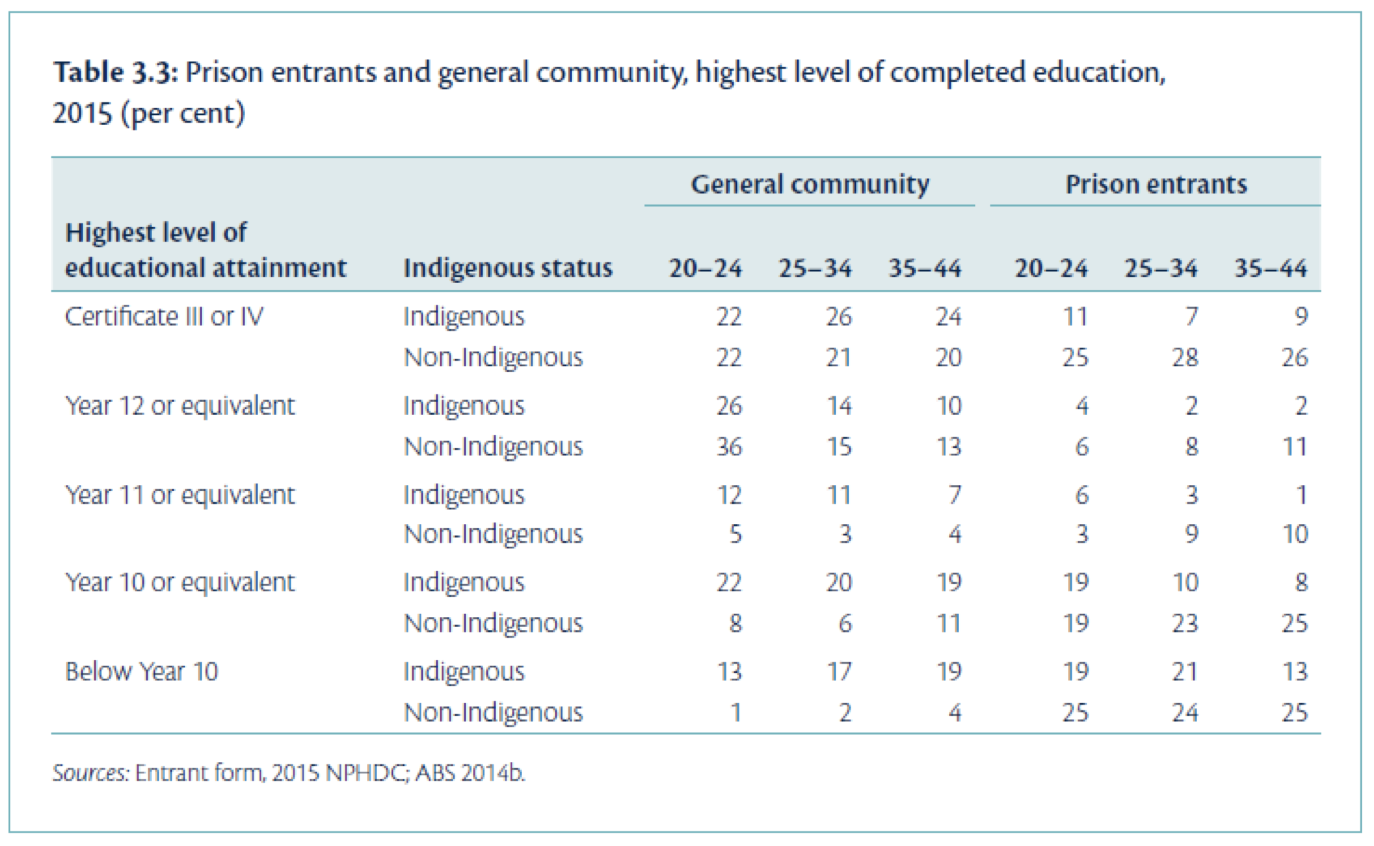
\includegraphics[width=0.66\textwidth,height=\textheight]{img/mod01/prisoner-education.png}

}

\caption{\label{fig-prison-education}Highest level of completed
education in prison entrants and the general community}

\end{figure}

Source: Australian Institute of Health and Welfare 2015. The health of
Australia's prisoners 2015. Cat. no. PHE 207. Canberra: AIHW.

Some issues in this table:

\begin{itemize}
\tightlist
\item
  The title of the table does not contain full information about the
  variables in the table;
\item
  It is unclear how the percentages were calculated (which groupings
  added to 100\%);
\item
  The ages are not labelled as such, thus without reading the text in
  report it is unclear that these are age groupings.
\end{itemize}

\hypertarget{summarising-two-categorical-variables-graphically}{%
\subsection{Summarising two categorical variables
graphically}\label{summarising-two-categorical-variables-graphically}}

Information from more than one variable can be presented as clustered or
multiple bar chart (bars side-by-side) (Figure~\ref{fig-bar-2}). This
type of graph is useful when examining changes in the categories
separately, but also comparing the grouping variable between the main
bar variable. Here we can see that Stage 3 and Stage 4 disease is the
most common for both males and females, but there are many more females
within each stage of disease.

\begin{figure}[H]

{\centering 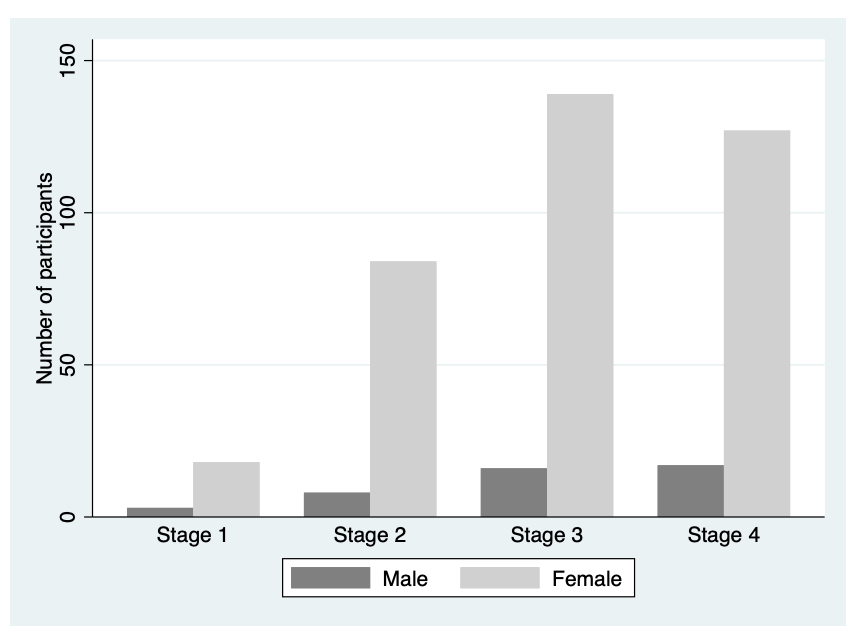
\includegraphics[width=0.75\textwidth,height=\textheight]{img/mod01/pbc-bar-stage-sex.png}

}

\caption{\label{fig-bar-2}Bar graph of stage of disease by sex from PBC
study}

\end{figure}

An alternative bar graph is a stacked or composite bar graph, which
retains the overall height for each category, but differentiates the
bars by another variable (Figure~\ref{fig-bar-3}).

\begin{figure}[H]

{\centering 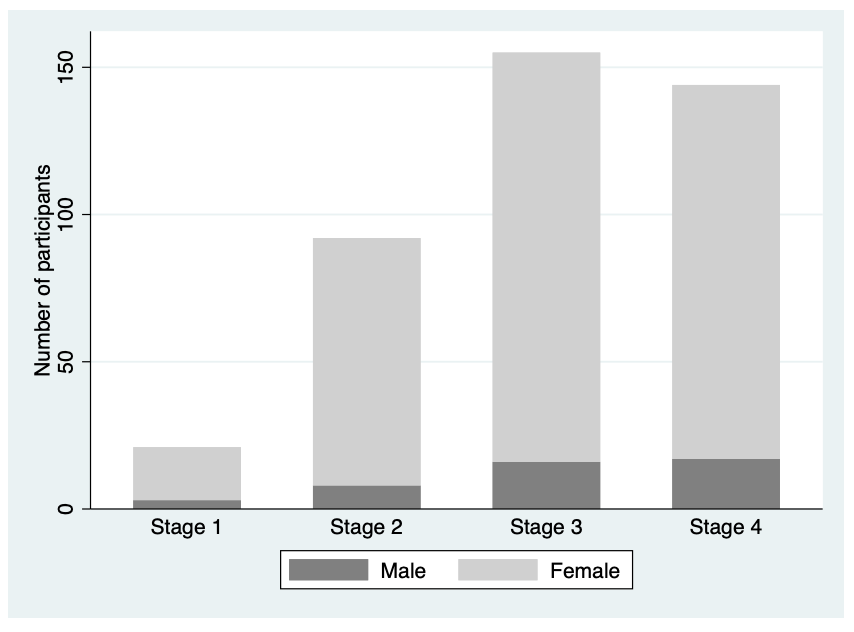
\includegraphics[width=0.75\textwidth,height=\textheight]{img/mod01/pbc-bar-stage-sex-stacked.png}

}

\caption{\label{fig-bar-3}Stacked bar graph of stage of disease by sex
from PBC study}

\end{figure}

Finally, a stacked relative bar chart (Figure~\ref{fig-bar-4}) displays
the proportion of grouping variable for each bar, where each overall bar
represents 100\%. These graphs allow the reader to compare the
proportions between categories. We can easily see from
Figure~\ref{fig-bar-4} that the distribution of sex is similar across
each stage of disease.

\begin{figure}[H]

{\centering 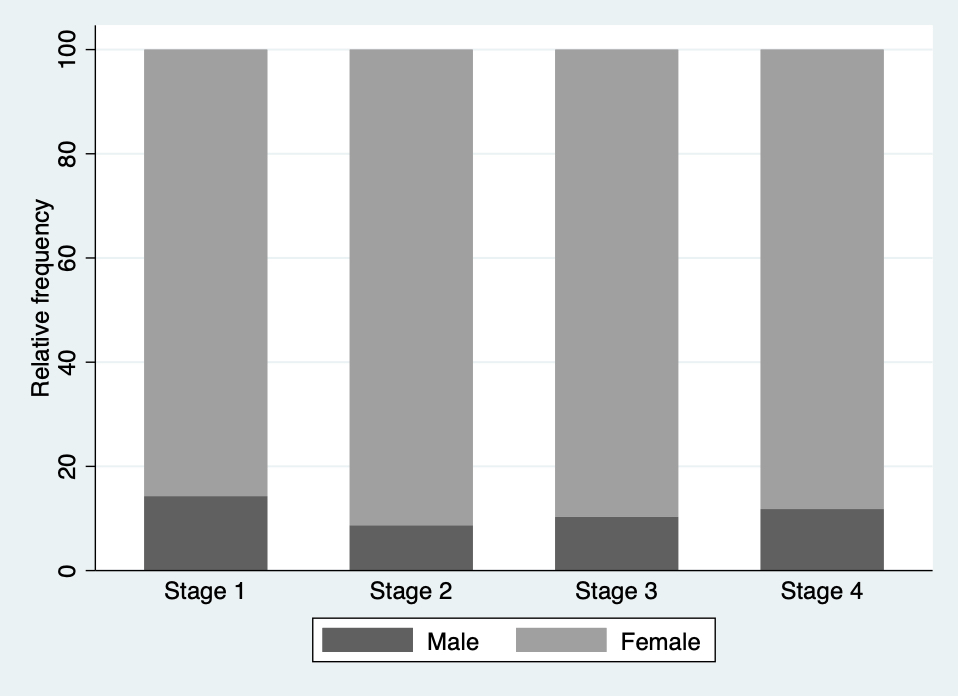
\includegraphics[width=0.75\textwidth,height=\textheight]{img/mod01/pbc-bar-stage-sex-stacked-relative.jpg}

}

\caption{\label{fig-bar-4}Relative frequency of sex within stage of
disease from PBC study}

\end{figure}

\hypertarget{line-graphs}{%
\subsection{Line graphs}\label{line-graphs}}

A line graph is effective to illustrate trends over time (e.g.~change
over several years). Let's look at an example from cancer epidemiology.

Cancer incidence is the number of new cases of cancer diagnosed in a
population in a given time period. A useful comparison with the
incidence rate is the mortality rate, revealing information about the
deaths from cancer in the same period. Figure~\ref{fig-line-1} shows the
prostate cancer trend in the NSW male population in the period
1972-2014, specifically the age-standardised incidence and mortality
rate per 100,000.

\begin{figure}[H]

{\centering 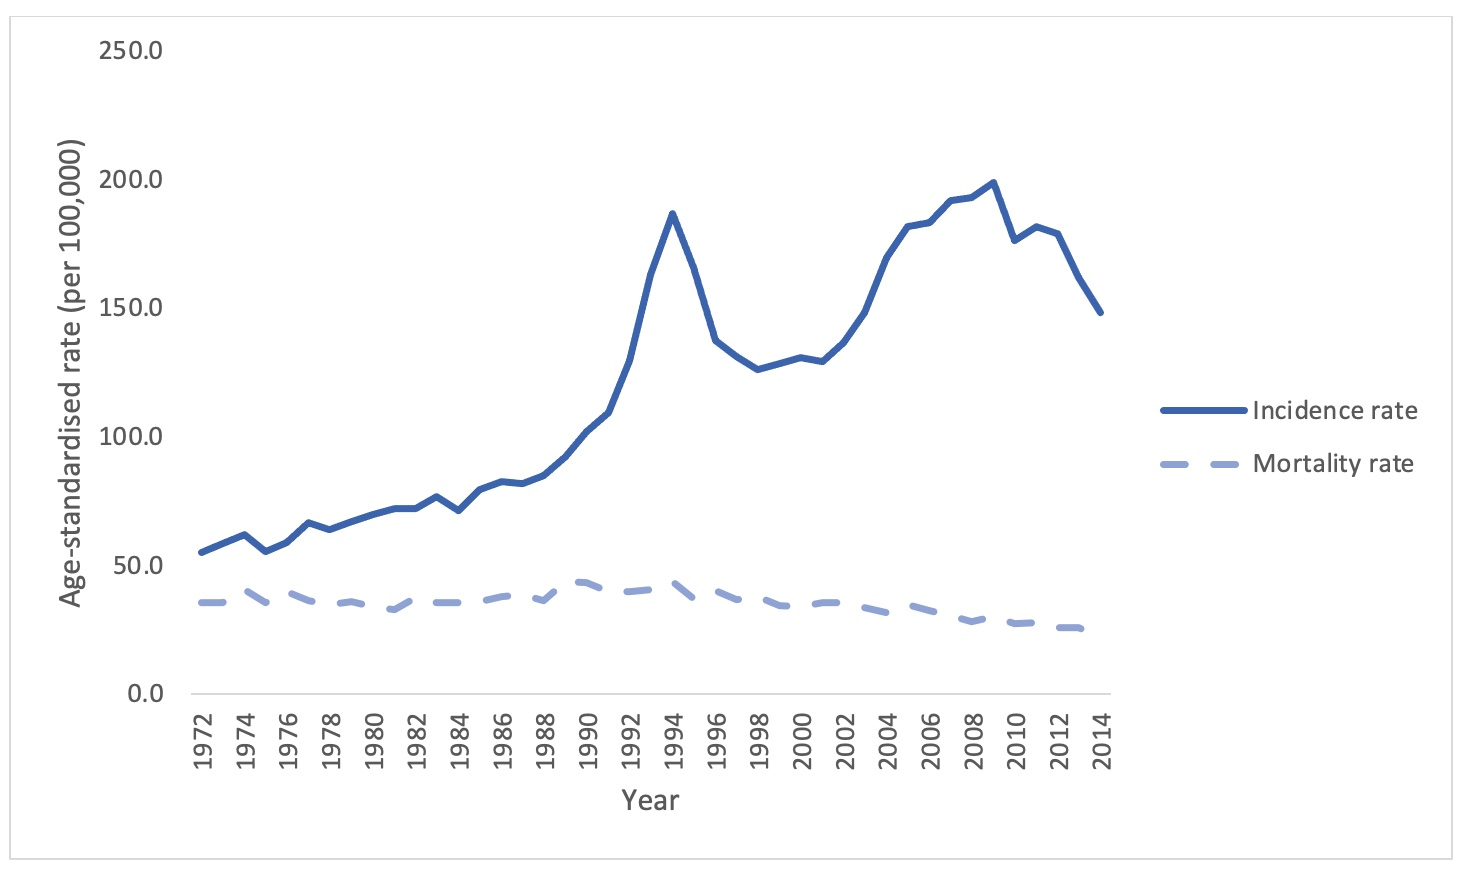
\includegraphics[width=0.66\textwidth,height=\textheight]{img/mod01/line-graph-prostate-cancer.jpg}

}

\caption{\label{fig-line-1}Prostate cancer age-standardised incidence
and mortality rates (per 100,000), NSW, 1972-2014}

\end{figure}

Source: The Cancer Institute NSW (2018) Cancer statistics NSW.
https://www.cancer.nsw.gov.au/cancer-statistics-nsw (Accessed: 24 Jan
2019).

The age standardised incidence rate for prostate cancer increased
steadily in the period 1972 -- 1991, from 55.2 cases per 100,00 to 109.3
cases per 100,000. There were two notable peaks in incidence in the
period 1972-2014. In particular, there was an increase between
1992-1994, and also between 2002-2009. Since 2009 (to 2014) the rates
decreased from 198.9 per 100,000 to 148.2 per 100,000. Whilst the
incidence rate for prostate cancer has fluctuated over the period, the
age standardised mortality rate remained relatively stable (around 35
deaths per 100,000). Since 2009 the mortality rate appears to be
decreasing and was at its lowest in 2014 at 22.1 per 100,000.

{[}The increase in prostate cancer incidence in the early 1990's
occurred at a time when blood testing of men for Prostate Specific
Antigen (PSA) became more widespread. The more recent peak in incidence
in the early 2000's maybe explained by PSA being increasingly used as a
screening test for men who did not have symptoms of prostate cancer.{]}

\hypertarget{presentation-guidelines}{%
\section{Presentation guidelines}\label{presentation-guidelines}}

\hypertarget{guidelines-for-presenting-summary-statistics}{%
\subsection{Guidelines for presenting summary
statistics}\label{guidelines-for-presenting-summary-statistics}}

When reporting summary statistics, it is important not to present
results with too many decimal places. Doing so implies that your data
have a higher level of precision than they do. For example, presenting a
mean blood pressure of 100.2487 mmHg implies that blood pressure can be
measured accurately to at least three decimal places.

There are a number of guidelines that have been written to help in the
presentation of numerical data. Many of these guidelines are based on
the number of decimal places, while others are based on the number of
significant figures. Briefly, the number of significant figures are
``the number of digits from the first non-zero digit to the last
meaningful digit, irrespective of the position of the decimal point.
Thus, 1.002, 10.02, 100200 (if this number is expressed to the nearest
100) all have four significant digits.'' Armitage, Berry, and Matthews
(2013)

A summary of these guidelines that will be used in this course appear in
Table~\ref{tbl-1-pres}.

\hypertarget{tbl-1-pres}{}
 
  \providecommand{\huxb}[2]{\arrayrulecolor[RGB]{#1}\global\arrayrulewidth=#2pt}
  \providecommand{\huxvb}[2]{\color[RGB]{#1}\vrule width #2pt}
  \providecommand{\huxtpad}[1]{\rule{0pt}{#1}}
  \providecommand{\huxbpad}[1]{\rule[-#1]{0pt}{#1}}

\begin{table}[ht]
\caption{\label{tbl-1-pres}Guidelines for presentation of statistical results }\tabularnewline

\begin{centerbox}
\begin{threeparttable}
 
\setlength{\tabcolsep}{0pt}
\begin{tabularx}{0.95\textwidth}{p{0.475\textwidth} p{0.475\textwidth}}


\hhline{>{\huxb{0, 0, 0}{0.4}}->{\huxb{0, 0, 0}{0.4}}-}
\arrayrulecolor{black}

\multicolumn{1}{!{\huxvb{0, 0, 0}{0}}m{0.475\textwidth}!{\huxvb{0, 0, 0}{0}}}{\hspace{0pt}\parbox[c]{0.475\textwidth-0pt-6pt}{\huxtpad{6pt + 1em}\raggedright \textbf{Summary statistic}\huxbpad{6pt}}} &
\multicolumn{1}{m{0.475\textwidth}!{\huxvb{0, 0, 0}{0}}}{\hspace{6pt}\parbox[c]{0.475\textwidth-6pt-0pt}{\huxtpad{6pt + 1em}\raggedright \textbf{Guideline (reference)}\huxbpad{6pt}}} \tabularnewline[-0.5pt]


\hhline{>{\huxb{0, 0, 0}{0.4}}->{\huxb{0, 0, 0}{0.4}}-}
\arrayrulecolor{black}

\multicolumn{1}{!{\huxvb{0, 0, 0}{0}}m{0.475\textwidth}!{\huxvb{0, 0, 0}{0}}}{\hspace{0pt}\parbox[c]{0.475\textwidth-0pt-6pt}{\huxtpad{6pt + 1em}\raggedright Mean\huxbpad{6pt}}} &
\multicolumn{1}{m{0.475\textwidth}!{\huxvb{0, 0, 0}{0}}}{\hspace{6pt}\parbox[c]{0.475\textwidth-6pt-0pt}{\huxtpad{6pt + 1em}\raggedright It is usually appropriate to quote the mean to one extra decimal place compared with the raw data. (Altman)\huxbpad{6pt}}} \tabularnewline[-0.5pt]


\hhline{}
\arrayrulecolor{black}

\multicolumn{1}{!{\huxvb{0, 0, 0}{0}}m{0.475\textwidth}!{\huxvb{0, 0, 0}{0}}}{\hspace{0pt}\parbox[c]{0.475\textwidth-0pt-6pt}{\huxtpad{6pt + 1em}\raggedright Median, Interquartile range, Range\huxbpad{6pt}}} &
\multicolumn{1}{m{0.475\textwidth}!{\huxvb{0, 0, 0}{0}}}{\hspace{6pt}\parbox[c]{0.475\textwidth-6pt-0pt}{\huxtpad{6pt + 1em}\raggedright As medians, interquartile ranges and ranges are based on individual data points, these values should be presented with the same precision as the original data.\huxbpad{6pt}}} \tabularnewline[-0.5pt]


\hhline{}
\arrayrulecolor{black}

\multicolumn{1}{!{\huxvb{0, 0, 0}{0}}m{0.475\textwidth}!{\huxvb{0, 0, 0}{0}}}{\hspace{0pt}\parbox[c]{0.475\textwidth-0pt-6pt}{\huxtpad{6pt + 1em}\raggedright Percentage\huxbpad{6pt}}} &
\multicolumn{1}{m{0.475\textwidth}!{\huxvb{0, 0, 0}{0}}}{\hspace{6pt}\parbox[c]{0.475\textwidth-6pt-0pt}{\huxtpad{6pt + 1em}\raggedright Percentages do not need to be given with more than one decimal place at most. When the sample size is less than 100, no decimal places should be given. (Altman)\huxbpad{6pt}}} \tabularnewline[-0.5pt]


\hhline{}
\arrayrulecolor{black}

\multicolumn{1}{!{\huxvb{0, 0, 0}{0}}m{0.475\textwidth}!{\huxvb{0, 0, 0}{0}}}{\hspace{0pt}\parbox[c]{0.475\textwidth-0pt-6pt}{\huxtpad{6pt + 1em}\raggedright Standard deviation\huxbpad{6pt}}} &
\multicolumn{1}{m{0.475\textwidth}!{\huxvb{0, 0, 0}{0}}}{\hspace{6pt}\parbox[c]{0.475\textwidth-6pt-0pt}{\huxtpad{6pt + 1em}\raggedright The standard deviation should usually be given to the same accuracy as the mean, or with one extra decimal place. (Altman)\huxbpad{6pt}}} \tabularnewline[-0.5pt]


\hhline{}
\arrayrulecolor{black}

\multicolumn{1}{!{\huxvb{0, 0, 0}{0}}m{0.475\textwidth}!{\huxvb{0, 0, 0}{0}}}{\hspace{0pt}\parbox[c]{0.475\textwidth-0pt-6pt}{\huxtpad{6pt + 1em}\raggedright Standard error\huxbpad{6pt}}} &
\multicolumn{1}{m{0.475\textwidth}!{\huxvb{0, 0, 0}{0}}}{\hspace{6pt}\parbox[c]{0.475\textwidth-6pt-0pt}{\huxtpad{6pt + 1em}\raggedright As per standard deviation\huxbpad{6pt}}} \tabularnewline[-0.5pt]


\hhline{}
\arrayrulecolor{black}

\multicolumn{1}{!{\huxvb{0, 0, 0}{0}}m{0.475\textwidth}!{\huxvb{0, 0, 0}{0}}}{\hspace{0pt}\parbox[c]{0.475\textwidth-0pt-6pt}{\huxtpad{6pt + 1em}\raggedright Confidence interval\huxbpad{6pt}}} &
\multicolumn{1}{m{0.475\textwidth}!{\huxvb{0, 0, 0}{0}}}{\hspace{6pt}\parbox[c]{0.475\textwidth-6pt-0pt}{\huxtpad{6pt + 1em}\raggedright Use the same rule as for the corresponding effect size (be it mean, percentage, mean difference, regression coefficient, correlation coefficient or risk ratio) (Cole)\huxbpad{6pt}}} \tabularnewline[-0.5pt]


\hhline{}
\arrayrulecolor{black}

\multicolumn{1}{!{\huxvb{0, 0, 0}{0}}m{0.475\textwidth}!{\huxvb{0, 0, 0}{0}}}{\hspace{0pt}\parbox[c]{0.475\textwidth-0pt-6pt}{\huxtpad{6pt + 1em}\raggedright Test statistic\huxbpad{6pt}}} &
\multicolumn{1}{m{0.475\textwidth}!{\huxvb{0, 0, 0}{0}}}{\hspace{6pt}\parbox[c]{0.475\textwidth-6pt-0pt}{\huxtpad{6pt + 1em}\raggedright Test statistics should not be presented with more than two decimal places.\huxbpad{6pt}}} \tabularnewline[-0.5pt]


\hhline{}
\arrayrulecolor{black}

\multicolumn{1}{!{\huxvb{0, 0, 0}{0}}m{0.475\textwidth}!{\huxvb{0, 0, 0}{0}}}{\hspace{0pt}\parbox[c]{0.475\textwidth-0pt-6pt}{\huxtpad{6pt + 1em}\raggedright P-value\huxbpad{6pt}}} &
\multicolumn{1}{m{0.475\textwidth}!{\huxvb{0, 0, 0}{0}}}{\hspace{6pt}\parbox[c]{0.475\textwidth-6pt-0pt}{\huxtpad{6pt + 1em}\raggedright Report p values to a single significant figure unless the p value is close to 0.05 (say, 0.01 – 0.2), in which case, report two significant figures. Do not report `not significant` for p values of 0.05 or higher. Very low p values can be reported as p $<$ 0.001 or similar. A p value can indeed be 1, although some investigators prefer to report this as $>$0.9. (Assel)\huxbpad{6pt}}} \tabularnewline[-0.5pt]


\hhline{}
\arrayrulecolor{black}

\multicolumn{1}{!{\huxvb{0, 0, 0}{0}}m{0.475\textwidth}!{\huxvb{0, 0, 0}{0}}}{\hspace{0pt}\parbox[c]{0.475\textwidth-0pt-6pt}{\huxtpad{6pt + 1em}\raggedright Difference in means\huxbpad{6pt}}} &
\multicolumn{1}{m{0.475\textwidth}!{\huxvb{0, 0, 0}{0}}}{\hspace{6pt}\parbox[c]{0.475\textwidth-6pt-0pt}{\huxtpad{6pt + 1em}\raggedright As for the estimated means\huxbpad{6pt}}} \tabularnewline[-0.5pt]


\hhline{}
\arrayrulecolor{black}

\multicolumn{1}{!{\huxvb{0, 0, 0}{0}}m{0.475\textwidth}!{\huxvb{0, 0, 0}{0}}}{\hspace{0pt}\parbox[c]{0.475\textwidth-0pt-6pt}{\huxtpad{6pt + 1em}\raggedright Difference in proportions\huxbpad{6pt}}} &
\multicolumn{1}{m{0.475\textwidth}!{\huxvb{0, 0, 0}{0}}}{\hspace{6pt}\parbox[c]{0.475\textwidth-6pt-0pt}{\huxtpad{6pt + 1em}\raggedright As for the estimated proportions\huxbpad{6pt}}} \tabularnewline[-0.5pt]


\hhline{}
\arrayrulecolor{black}

\multicolumn{1}{!{\huxvb{0, 0, 0}{0}}m{0.475\textwidth}!{\huxvb{0, 0, 0}{0}}}{\hspace{0pt}\parbox[c]{0.475\textwidth-0pt-6pt}{\huxtpad{6pt + 1em}\raggedright Odds ratio / Relative risk\huxbpad{6pt}}} &
\multicolumn{1}{m{0.475\textwidth}!{\huxvb{0, 0, 0}{0}}}{\hspace{6pt}\parbox[c]{0.475\textwidth-6pt-0pt}{\huxtpad{6pt + 1em}\raggedright Hazard and odds ratios are normally reported to two decimal places, although this can be avoided for high odds ratios (Assel)\huxbpad{6pt}}} \tabularnewline[-0.5pt]


\hhline{}
\arrayrulecolor{black}

\multicolumn{1}{!{\huxvb{0, 0, 0}{0}}m{0.475\textwidth}!{\huxvb{0, 0, 0}{0}}}{\hspace{0pt}\parbox[c]{0.475\textwidth-0pt-6pt}{\huxtpad{6pt + 1em}\raggedright Correlation coefficient\huxbpad{6pt}}} &
\multicolumn{1}{m{0.475\textwidth}!{\huxvb{0, 0, 0}{0}}}{\hspace{6pt}\parbox[c]{0.475\textwidth-6pt-0pt}{\huxtpad{6pt + 1em}\raggedright One or two decimal places, or more when very close to ±1   (Cole)\huxbpad{6pt}}} \tabularnewline[-0.5pt]


\hhline{}
\arrayrulecolor{black}

\multicolumn{1}{!{\huxvb{0, 0, 0}{0}}m{0.475\textwidth}!{\huxvb{0, 0, 0}{0}}}{\hspace{0pt}\parbox[c]{0.475\textwidth-0pt-6pt}{\huxtpad{6pt + 1em}\raggedright Regression coefficient\huxbpad{6pt}}} &
\multicolumn{1}{m{0.475\textwidth}!{\huxvb{0, 0, 0}{0}}}{\hspace{6pt}\parbox[c]{0.475\textwidth-6pt-0pt}{\huxtpad{6pt + 1em}\raggedright Use one more significant figure than the underlying data   (adapted from Cole)\huxbpad{6pt}}} \tabularnewline[-0.5pt]


\hhline{>{\huxb{0, 0, 0}{0.4}}->{\huxb{0, 0, 0}{0.4}}-}
\arrayrulecolor{black}
\end{tabularx}
\end{threeparttable}\par\end{centerbox}

\end{table}
 

\hypertarget{table-presentation-guidelines}{%
\subsection{Table presentation
guidelines}\label{table-presentation-guidelines}}

Consider the following guidelines for the appropriate presentation of
tables in scientific journals and reports (Woodward, 2013).

\begin{enumerate}
\def\labelenumi{\arabic{enumi}.}
\tightlist
\item
  Each table (and figure) should be self-explanatory, i.e.~the reader
  should be able to understand it without reference to the text in the
  body of the report.

  \begin{itemize}
  \tightlist
  \item
    This can be achieved by using complete, meaningful labels for the
    rows and columns and giving a complete, meaningful title.
  \item
    Footnotes can be used to enhance the explanation.
  \end{itemize}
\item
  Units of the variables (and if needed, method of calculation or
  derivation) should be given and missing records should be noted
  (e.g.~in a footnote).
\item
  A table should be visually uncluttered.

  \begin{itemize}
  \tightlist
  \item
    Avoid use of vertical lines.
  \item
    Horizontal lines should not be used in every single row, but they
    can be used to group parts of the table.
  \item
    Sensible use of white space also helps enormously; use equal spacing
    except where large spaces are left to separate distinct parts of the
    table.
  \item
    Different typefaces (or fonts) may be used to provide
    discrimination, e.g.~use of bold type and/or italics.
  \end{itemize}
\item
  The rows and columns of each table should be arranged in a natural
  order to help interpretation. For instance, when rows are ordered by
  the size of the numbers they contain for a nominal variable, it is
  immediately obvious where relatively big and small contributions come
  from.
\item
  Tables should have a consistent appearance throughout the report so
  that the paper is easy to follow (and also for an aesthetic
  appearance). Conventions for labelling and ordering should be the same
  (for both tables as well as figures) for ease of comparison of
  different tables (and figures).
\item
  Consider if there is a particular table orientation that makes a table
  easier to read.
\end{enumerate}

Given the different possible formats of tables and their complexity,
some further guidelines are given in the following excellent references:

\begin{itemize}
\tightlist
\item
  Graphics and statistics for cardiology: designing effective tables for
  presentation and publication, Boers (2018)
\item
  Guidelines for Reporting of Figures and Tables for Clinical Research
  in Urology, Vickers et al. (2020)
\end{itemize}

\hypertarget{graphical-presentation-guidelines}{%
\subsection{Graphical presentation
guidelines}\label{graphical-presentation-guidelines}}

Consider the following guidelines for the appropriate presentation of
graphs in scientific journals and reports (Woodward, 2013).

\begin{itemize}
\tightlist
\item
  Figures should be self-explanatory and have consistent appearance
  through the report.
\item
  A title should give complete information. Note that figure titles are
  usually placed below the figure, whereas for tables titles are given
  above the table.
\item
  Axes should be labelled appropriately
\item
  Units of the variables should be given in the labelling of the axes.
  Use footnotes to indicate any calculation or derivation of variables
  and to indicate missing values
\item
  If the Y-axis has a natural origin, it should be included, or
  emphasised if it is not included.
\item
  If graphs are being compared, the Y-axis should be the same across the
  graphs to enable fair comparison
\item
  Columns of bar charts should be separated by a space
\item
  Three dimensional graphs should be avoided unless the third dimension
  adds additional information
\end{itemize}

Sources:

Altman (1990)

Cole (2015)

Assel et al. (2019)

\newpage{}

\bookmarksetup{startatroot}

\hypertarget{an-introduction-to-stata}{%
\chapter*{An introduction to Stata}\label{an-introduction-to-stata}}
\addcontentsline{toc}{chapter}{An introduction to Stata}

\markboth{An introduction to Stata}{An introduction to Stata}

\hypertarget{learning-outcomes-1}{%
\section*{Learning outcomes}\label{learning-outcomes-1}}
\addcontentsline{toc}{section}{Learning outcomes}

\markright{Learning outcomes}

By the end of these notes, you will be able to:

\begin{itemize}
\tightlist
\item
  navigate the Stata interface
\item
  input and import data into Stata
\item
  use Stata menus to summarise data
\item
  perform basic data transformations
\item
  assign variable and value labels
\item
  understand the difference between saving data and saving Stata output
\item
  copy Stata output to a standard word processing package
\end{itemize}

\hypertarget{introduction}{%
\section{Introduction}\label{introduction}}

Stata is a powerful statistical package that is relatively easy to use.
It is commonly used in health research, as well as in other fields such
as econometrics and social science. The aim of these notes is to
introduce the Stata environment, and to introduce the commands and
procedures that are directly relevant to this course. There is much more
to Stata that we will cover in these notes, and more information will be
provided throughout the course.

\hypertarget{part-1-a-simple-stata-analysis}{%
\section{Part 1: A simple Stata
analysis}\label{part-1-a-simple-stata-analysis}}

In this very brief section, we will introduce Stata by calculating the
average of six ages. If you are using Windows, open Stata by clicking:
\textbf{Start \textgreater{} Stata 18 \textgreater{} Stata SE}

If you are using MacOS, open Stata from the Applications folder. Note
that while Stata is available for Windows and MacOS, most of the
screenshots in these notes will be based on the Windows version.

Alternatively, open Stata using UNSW's myAccess service.

When you first open Stata, it will look something like the following.

\begin{figure}[H]

{\centering 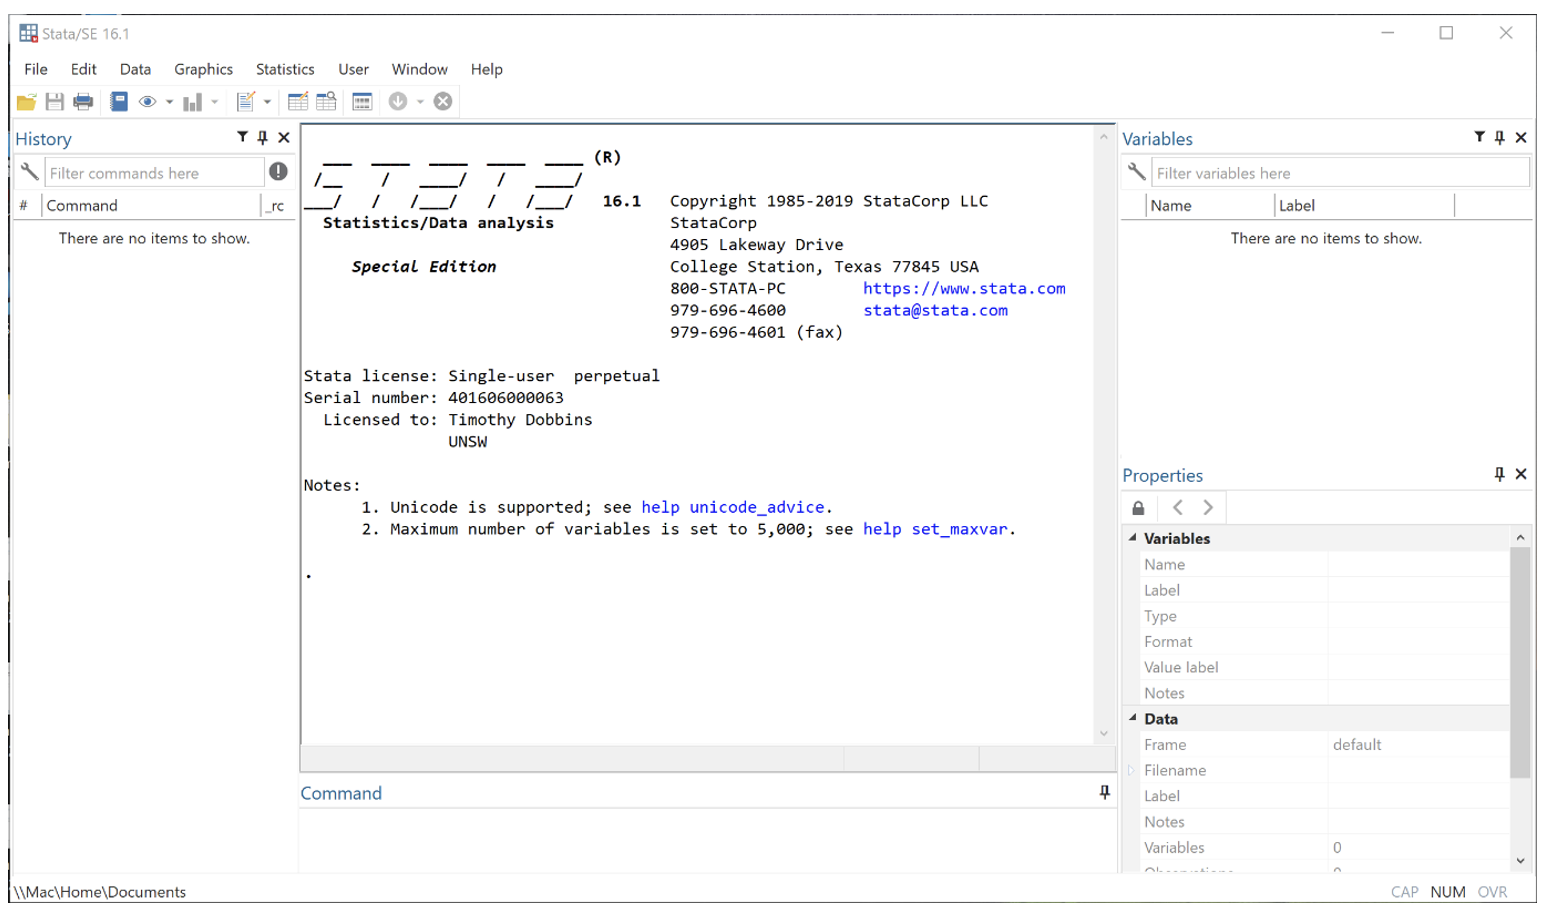
\includegraphics[width=0.75\textwidth,height=\textheight]{img/mod01/stata/simple-01.png}

}

\end{figure}

Each Stata session has a number of windows, which we will discuss later.
For now, look in the top row of icons and find the icons that look like
two grids: one with a pencil, and one with a magnifying glass:

\includegraphics{img/mod01/stata/data-browser-icons.png}. Click the left
icon, the one with the pencil. The following window will appear.

\begin{figure}[H]

{\centering 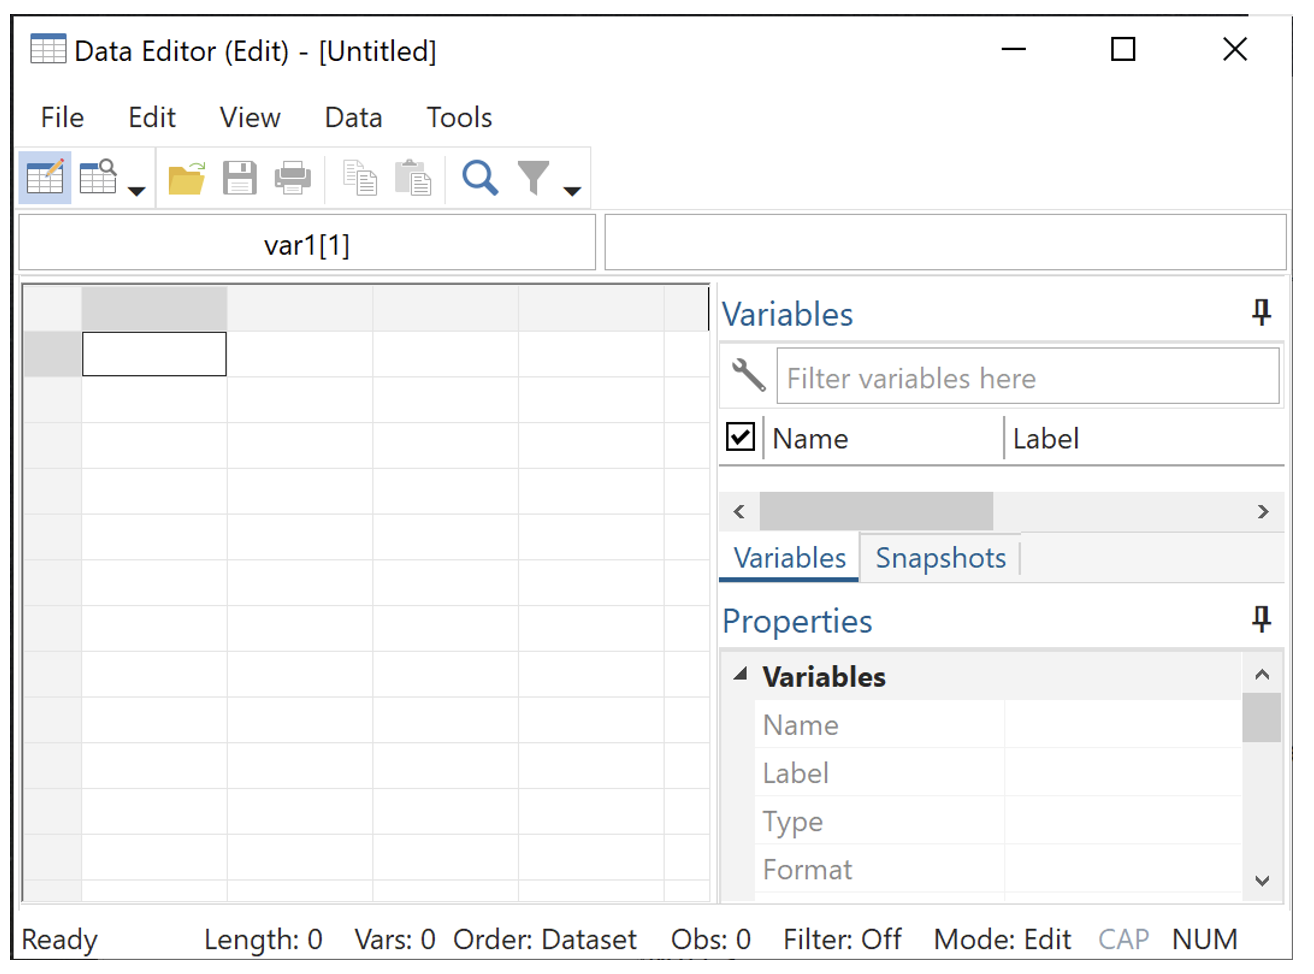
\includegraphics[width=0.75\textwidth,height=\textheight]{img/mod01/stata/simple-02.png}

}

\end{figure}

This window is known as the \textbf{Data Editor}, and is where data can
be entered or changed.

\begin{tcolorbox}[enhanced jigsaw, title={TASK}, opacitybacktitle=0.6, colbacktitle=quarto-callout-note-color!10!white, titlerule=0mm, colframe=quarto-callout-note-color-frame, opacityback=0, left=2mm, breakable, bottomtitle=1mm, coltitle=black, bottomrule=.15mm, arc=.35mm, rightrule=.15mm, toptitle=1mm, colback=white, toprule=.15mm, leftrule=.75mm]

Enter the following six ages into Stata, starting at the top-left cell,
by typing each number and then hitting Enter:

\texttt{20\ 25\ \ 23\ \ 29\ \ 21\ \ 27}

If you make a mistake, simply click the incorrect cell, and enter the
correct value.

\end{tcolorbox}

Your screen should look like this:

\begin{figure}[H]

{\centering 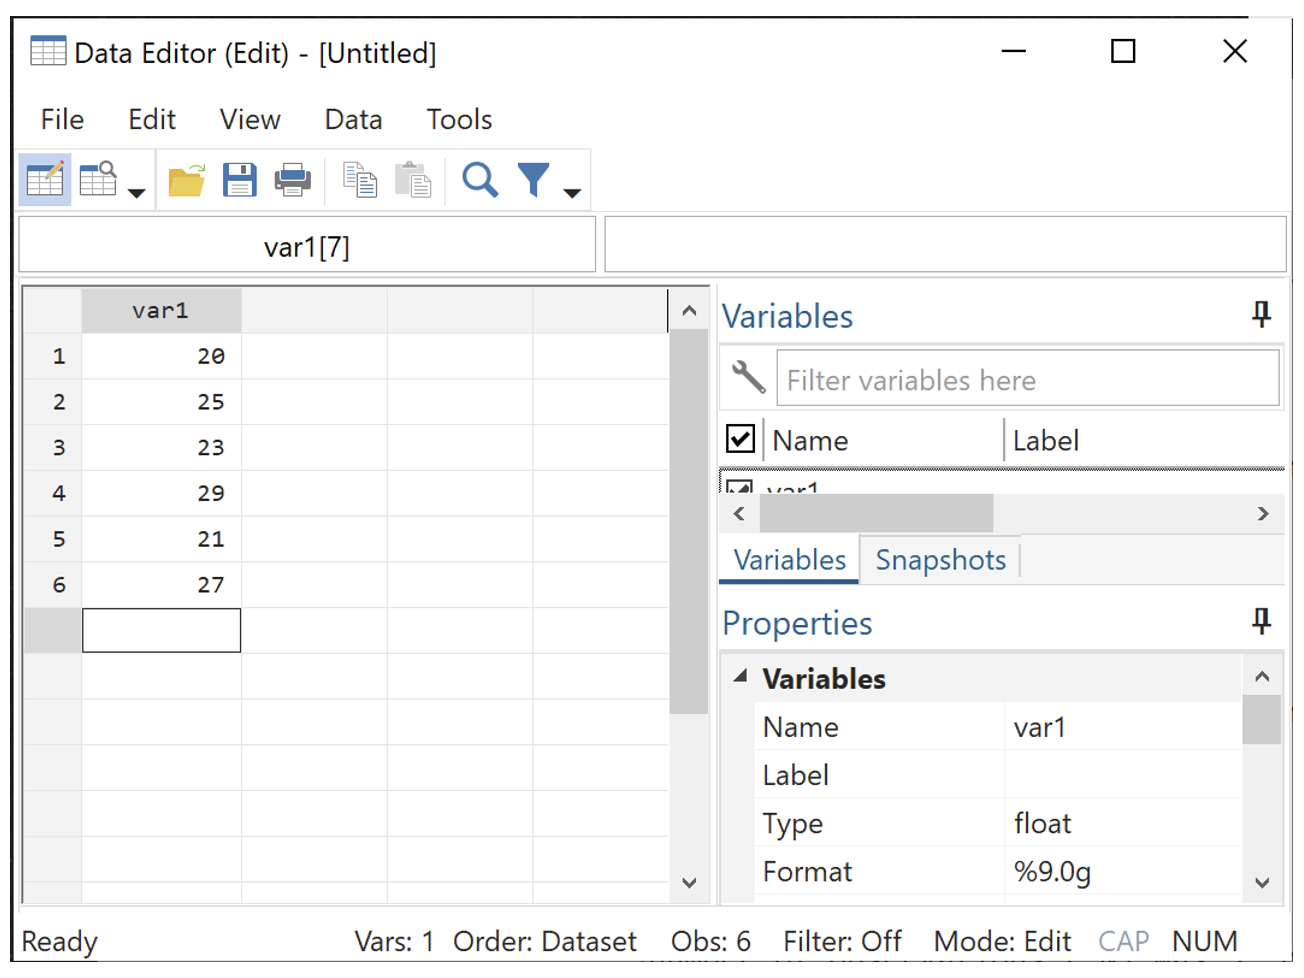
\includegraphics[width=0.75\textwidth,height=\textheight]{img/mod01/stata/simple-03.png}

}

\end{figure}

There are two things to note here:

\begin{enumerate}
\def\labelenumi{\arabic{enumi}.}
\tightlist
\item
  Data in Stata are entered down a column. In Stata, columns represent
  variables, and rows represent observations. So our six observations of
  age are entered in one column.
\item
  Stata has given the name of \texttt{var1} to our column of ages. We
  will fix this in a moment.
\end{enumerate}

Close the \textbf{Data Editor} window to return to the main Stata
window. You will notice that the main Stata window now has some text
that you might not understand. We will explain why shortly.

Let's rename our variable from \texttt{var1} to \texttt{age}. There are
a few ways you can do this in Stata, but one of the most convenient is
to use the \textbf{Variables Manager} which can be accessed via
\textbf{Data \textgreater{} Variables Manager}:

\begin{figure}[H]

{\centering 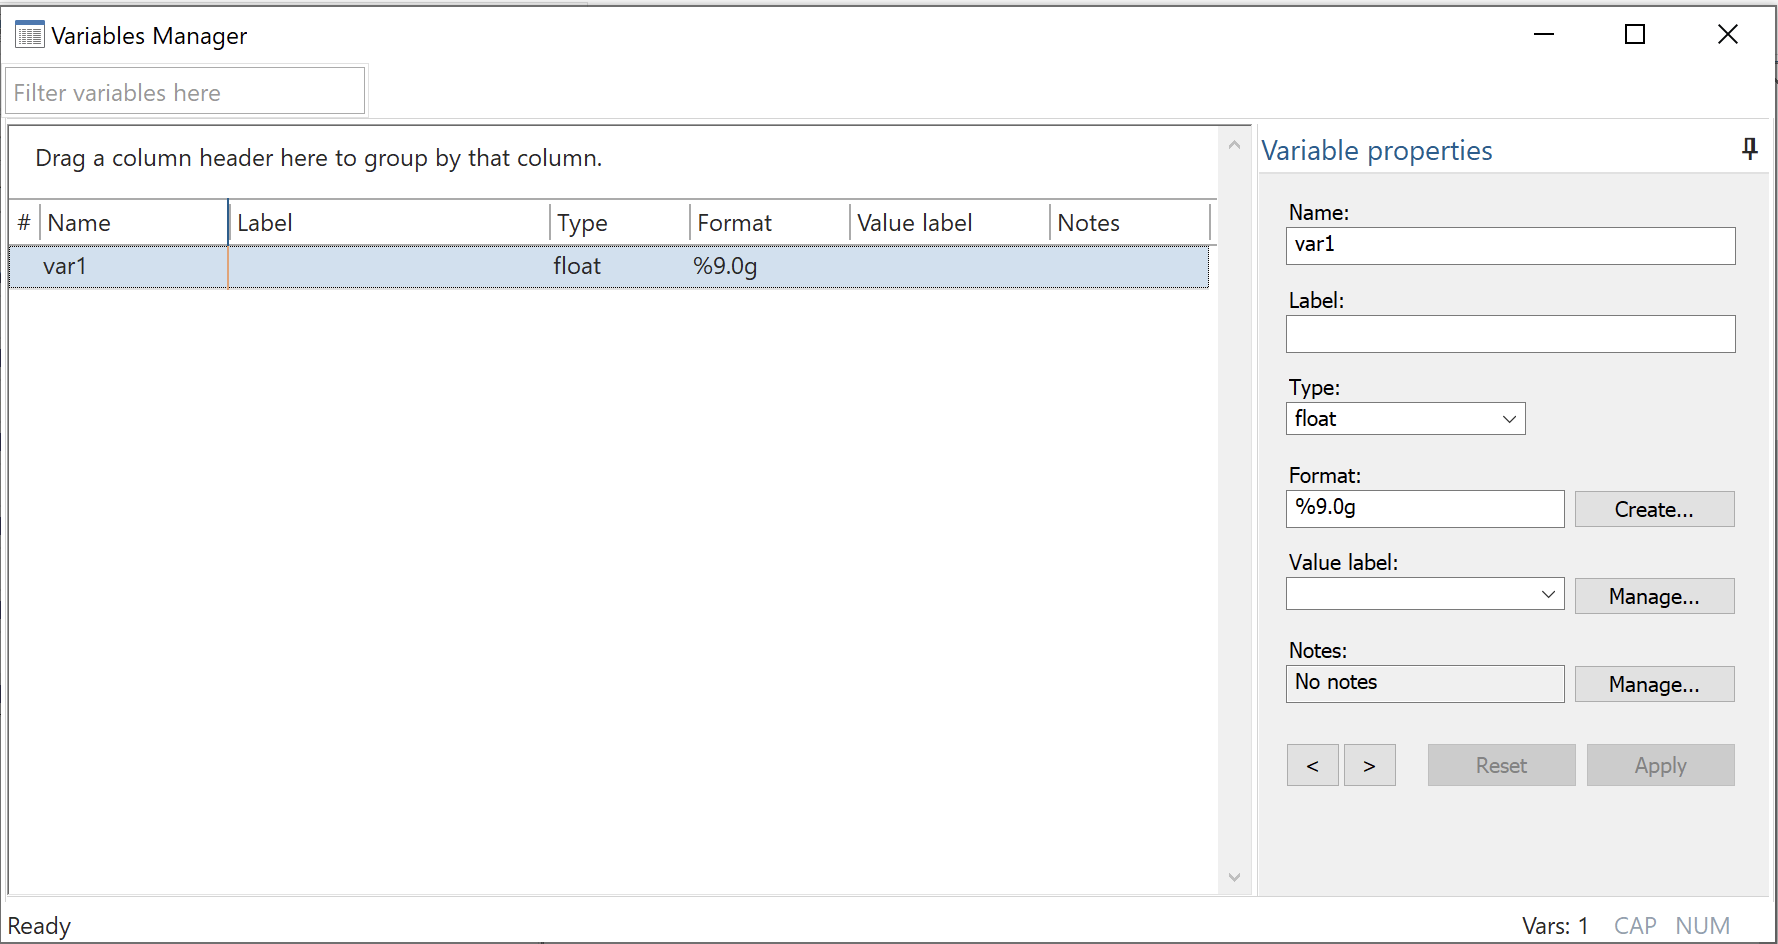
\includegraphics[width=0.75\textwidth,height=\textheight]{img/mod01/stata/variables-manager-01.png}

}

\end{figure}

The \textbf{Variables Manager} is where you can change many variable
properties, such as variable names or apply meaningful variable labels.
Each variable is listed on a separate row, with aspects about each
variable listed in the columns. To change the variable name, click
\texttt{var1} in the \textbf{Name} column. Notice that information about
that variable appears to the right of the window, in the
\textbf{Variable properties} section.

In the \textbf{Name} section within \textbf{Variable properties}, click
\texttt{var1} and replace it with \texttt{age}. Click \textbf{Apply} and
notice that the variable's name has been changed:

\begin{figure}[H]

{\centering 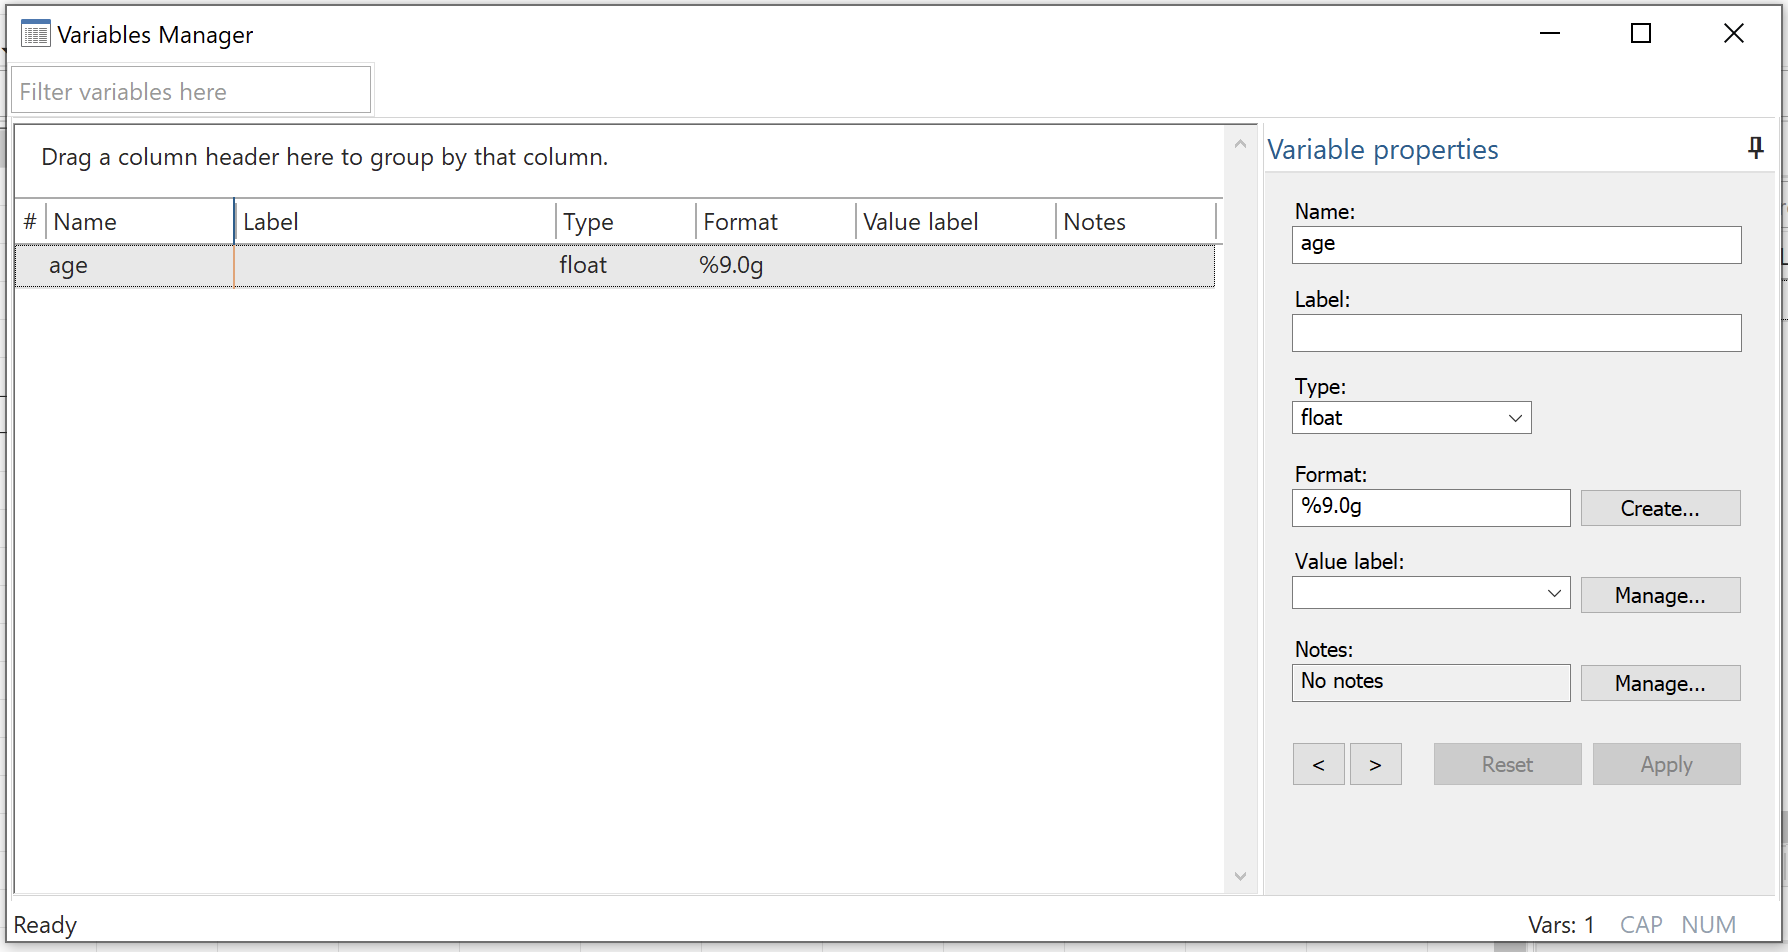
\includegraphics[width=0.75\textwidth,height=\textheight]{img/mod01/stata/variables-manager-02.png}

}

\end{figure}

Close the \textbf{Variables manager} window.

Some important points about variable names in Stata:

\begin{itemize}
\tightlist
\item
  any name you choose must be no more than 32 characters long;
\item
  variable names must contain only letters, numbers and the underscore
  (\_);
\item
  variable names should start with a letter;
\item
  variable names are case-sensitive (so age, Age and AGE could represent
  three different variables)
\end{itemize}

\begin{tcolorbox}[enhanced jigsaw, title={TASK}, opacitybacktitle=0.6, colbacktitle=quarto-callout-note-color!10!white, titlerule=0mm, colframe=quarto-callout-note-color-frame, opacityback=0, left=2mm, breakable, bottomtitle=1mm, coltitle=black, bottomrule=.15mm, arc=.35mm, rightrule=.15mm, toptitle=1mm, colback=white, toprule=.15mm, leftrule=.75mm]

Rename the variable \texttt{\_var1} with the name \texttt{age}.

\end{tcolorbox}

Now that we have entered our six ages, let's calculate the mean age.
Choose \textbf{Statistics \textgreater{} Summaries, tables and tests
\textgreater{} Summary and descriptive statistics \textgreater{} Summary
statistics}. The \textbf{summarize} dialog box will appear. From the
\textbf{Variables} drop-down box, select \texttt{age} as below:

\begin{figure}[H]

{\centering 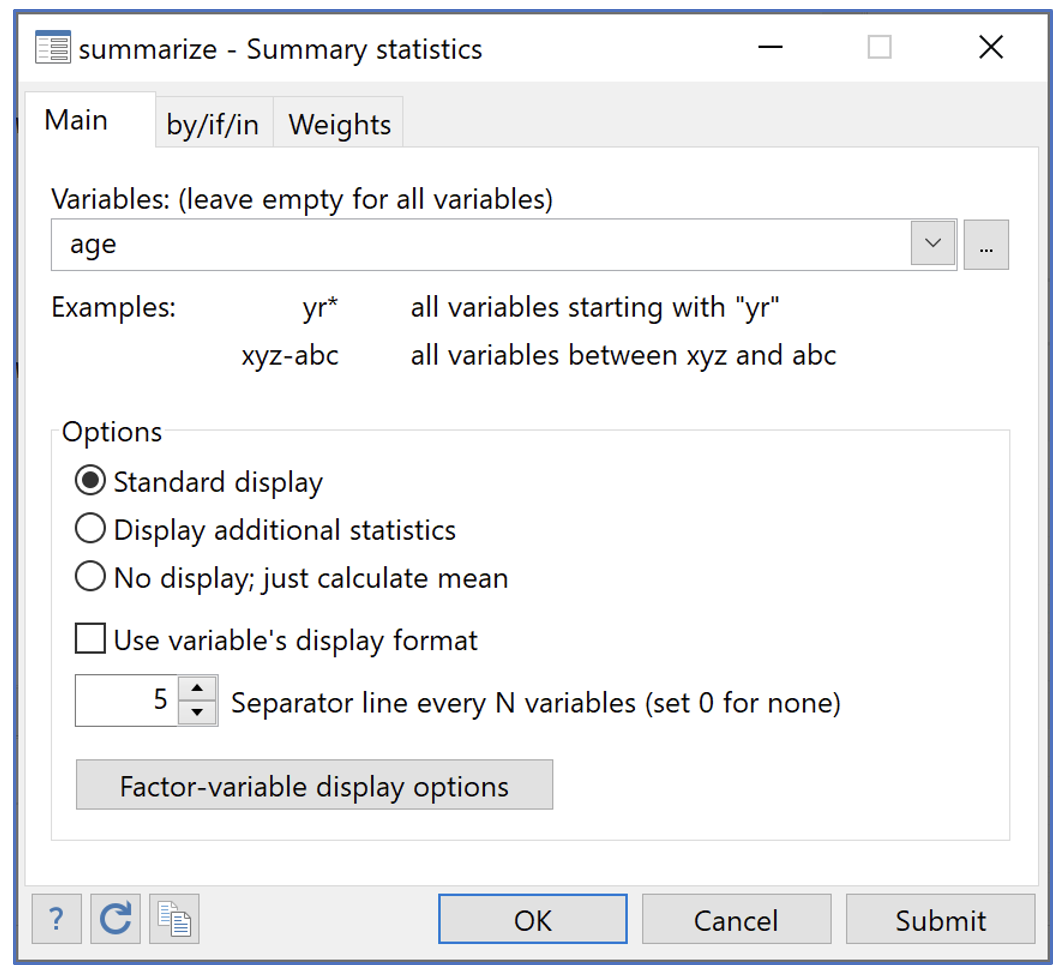
\includegraphics[width=0.75\textwidth,height=\textheight]{img/mod01/stata/simple-05.png}

}

\end{figure}

Click \textbf{OK}, and the main Stata screen will appear as below.

\begin{figure}[H]

{\centering 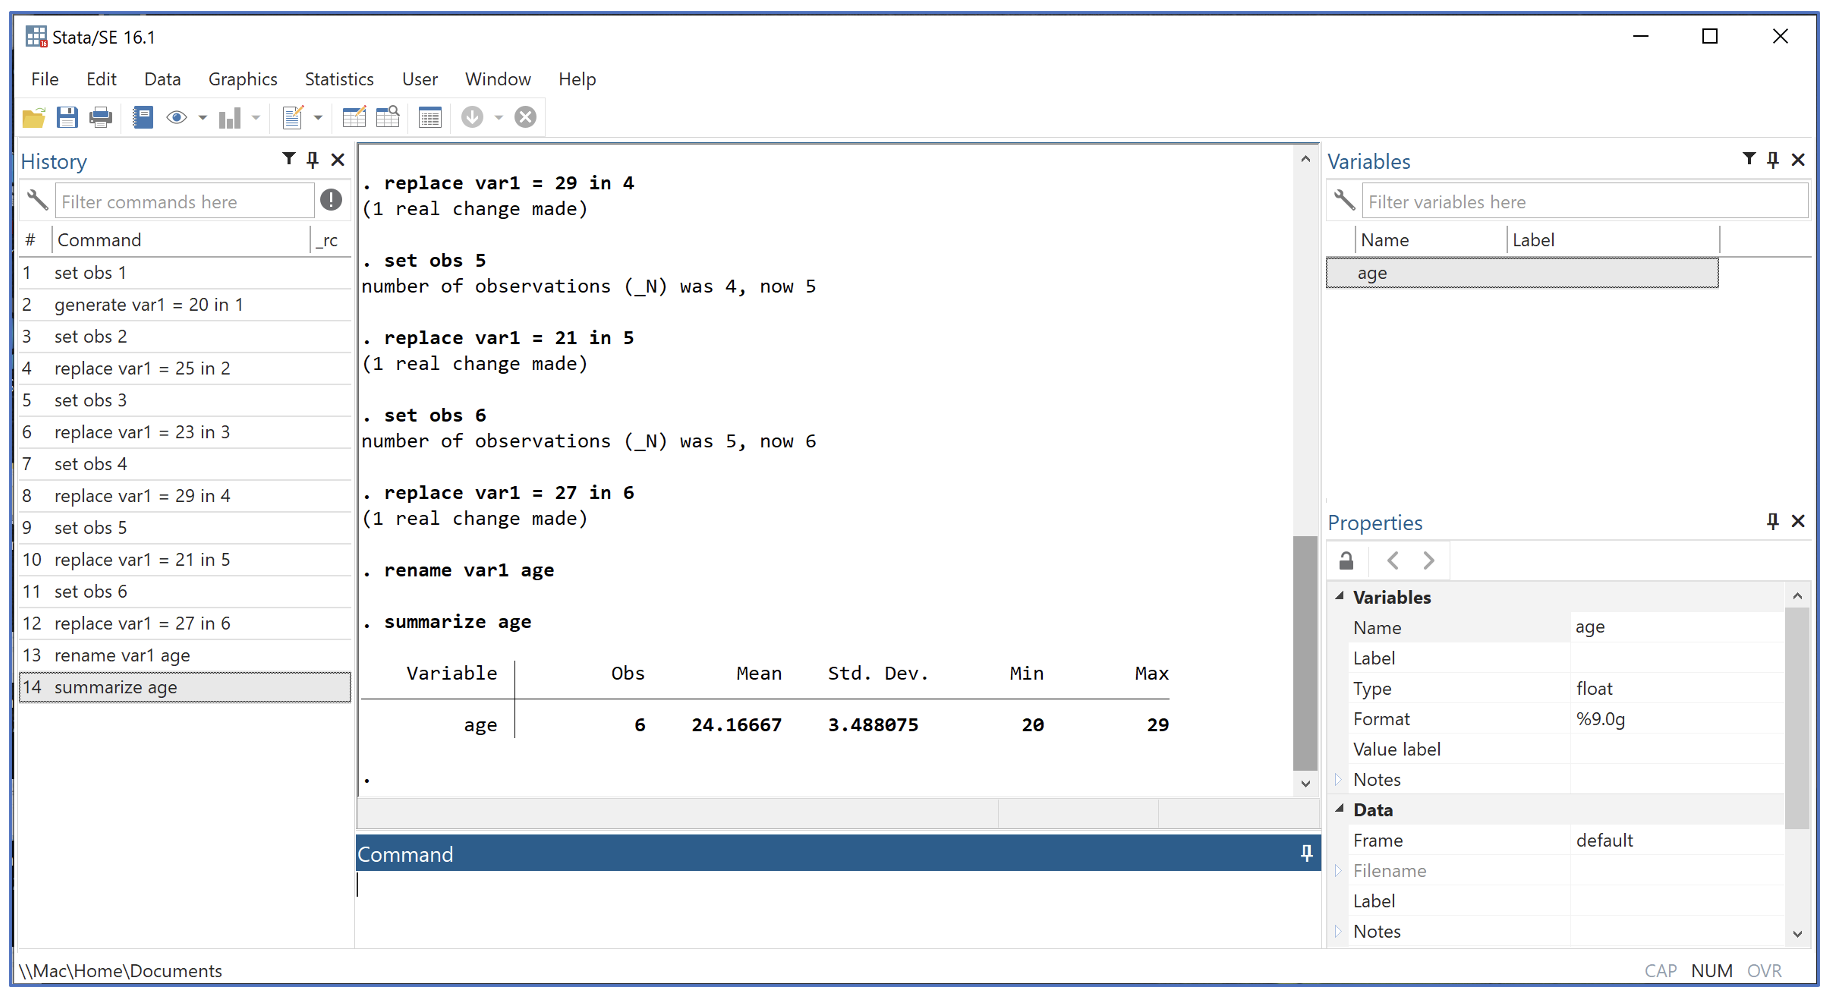
\includegraphics[width=0.75\textwidth,height=\textheight]{img/mod01/stata/simple-06.png}

}

\end{figure}

\begin{tcolorbox}[enhanced jigsaw, title={TASK}, opacitybacktitle=0.6, colbacktitle=quarto-callout-note-color!10!white, titlerule=0mm, colframe=quarto-callout-note-color-frame, opacityback=0, left=2mm, breakable, bottomtitle=1mm, coltitle=black, bottomrule=.15mm, arc=.35mm, rightrule=.15mm, toptitle=1mm, colback=white, toprule=.15mm, leftrule=.75mm]

Calculate summary statisitics for \texttt{age} and confirm: there are 6
observations, with a mean age of 24.2 years, a standard deviation of
3.49 years, a minimum of 20 and a maximum of 29 years.

\end{tcolorbox}

\hypertarget{the-stata-environment}{%
\subsection{The Stata environment}\label{the-stata-environment}}

Now that we have seen a simple example of how to use Stata, let's
describe the Stata environment. The largest window in Stata is the
\textbf{Results} window. This is where the results of your analyses
appear, as well as any information, warnings or error messages. You may
have noticed that the \textbf{Results} window also contains commands
used to conduct analyses. For example, there is a command above summary
output for age:

\texttt{.\ summarize\ age}

This command is generated by Stata based on the entries in the
\textbf{summarize} dialog box. Stata is inherently a command-driven
program: the menus and dialog boxes simply generate commands that Stata
interprets, and these commands (and their results) are included in the
Results window. While most menu items and dialog boxes can be replicated
using commands, it is easier to learn Stata using the menus and dialog
boxes. In later Modules, we will include the commands that can be used
as alternatives to using the Stata menus.

The Stata windows are summarised below.

\begin{longtable}[]{@{}
  >{\raggedright\arraybackslash}p{(\columnwidth - 2\tabcolsep) * \real{0.5000}}
  >{\raggedright\arraybackslash}p{(\columnwidth - 2\tabcolsep) * \real{0.5000}}@{}}
\toprule\noalign{}
\begin{minipage}[b]{\linewidth}\raggedright
Window
\end{minipage} & \begin{minipage}[b]{\linewidth}\raggedright
Purpose
\end{minipage} \\
\midrule\noalign{}
\endhead
\bottomrule\noalign{}
\endlastfoot
Results & Shows your issued commands, results output (e.g.~tables) and
error messages or warnings. \\
Command & Where you can type in a command you want to run. The command
window need not be used in this course \\
Variables & Gives a list of the variables in your currently opened
dataset. \\
Properties & Shows the properties of your currently selected variable
(selected from the Variables window) and of your currently opened
dataset. \\
History & Shows the history of your issued commands in your current
session. \\
Data Editor (Edit) & A separate window that allows you to edit or enter
data. \\
Data Editor (Browse) & A separate window that allows you to view data:
data cannot be edited. \\
\end{longtable}

Stata allows you to perform most of your work by selecting options from
the appropriate menus at the top of the main Stata window. A brief
description of the main menu bar options follows.

\textbf{File} includes all the options you typically use in other
programs, such as Open, Save, Exit. Note, that you can open or create
various types of new files. The main type of file we open or create in
this course is a Stata data file (.dta). In the Advanced Biostatistics
and Statistical Computing course (PHCM9517), we will also use other file
types such as a .do file for scripting (or writing) Stata commands.

\textbf{Edit} includes the typical Copy, and Paste commands.

\textbf{Data} allows you to open the \textbf{Data Editor}. You can also
create new variables and change current variables using \textbf{Data
\textgreater{} Create or change data}.

\textbf{Graphics} includes the commands to create various types of
graphs including box plots, histograms, scatterplots, line graphs, and
bar charts.

\textbf{Statistics} includes all the commands to carry out statistical
analyses and perform power and sample size calculations. Much of this
course will focus on using commands located in this menu.

\textbf{User} is for saved files from other windows (e.g.~saved graphs).
You will not need to use this option in this course.

\textbf{Window} can be used to select which window you want to view
(e.g.~Results, Data Editor).

\textbf{Help} has many useful options including the viewing the PDF
documentation, a Search function and other resources for using Stata. We
will also demonstrate how to use helpful resources later in this
introductory manual. Another useful Stata resource is the video
tutorials produced by Stata:
https://www.stata.com/links/video-tutorials/

\hypertarget{part-2-obtaining-basic-descriptive-statistics}{%
\section{Part 2: Obtaining basic descriptive
statistics}\label{part-2-obtaining-basic-descriptive-statistics}}

In this exercise, we will analyse data to complete a descriptive table
from a research study. The data come from a study in primary biliary
cirrhosis, a condition of the liver, from Therneau and Grambsch (2010),
Modeling Survival Data: Extending the Cox Model. By the end of this
exercise, we will have completed the following table.

 
  \providecommand{\huxb}[2]{\arrayrulecolor[RGB]{#1}\global\arrayrulewidth=#2pt}
  \providecommand{\huxvb}[2]{\color[RGB]{#1}\vrule width #2pt}
  \providecommand{\huxtpad}[1]{\rule{0pt}{#1}}
  \providecommand{\huxbpad}[1]{\rule[-#1]{0pt}{#1}}

\begin{table}[ht]
\caption{Summary of 418 participants from the PBC study (Therneau and Grambsch,
2000)}\tabularnewline

\begin{centerbox}
\begin{threeparttable}
 \setlength{\tabcolsep}{0pt}
\begin{tabularx}{0.95\textwidth}{p{0.316666666666667\textwidth} p{0.316666666666667\textwidth} p{0.316666666666667\textwidth}}


\hhline{>{\huxb{0, 0, 0}{0.4}}->{\huxb{0, 0, 0}{0.4}}->{\huxb{0, 0, 0}{0.4}}-}
\arrayrulecolor{black}

\multicolumn{1}{!{\huxvb{0, 0, 0}{0}}p{0.316666666666667\textwidth}!{\huxvb{0, 0, 0}{0}}}{\hspace{0pt}\parbox[b]{0.316666666666667\textwidth-0pt-6pt}{\huxtpad{6pt + 1em}\raggedright \textbf{Characteristic}\huxbpad{6pt}}} &
\multicolumn{1}{p{0.316666666666667\textwidth}!{\huxvb{0, 0, 0}{0}}}{\hspace{6pt}\parbox[b]{0.316666666666667\textwidth-6pt-6pt}{\huxtpad{6pt + 1em}\raggedright \textbf{ }\huxbpad{6pt}}} &
\multicolumn{1}{p{0.316666666666667\textwidth}!{\huxvb{0, 0, 0}{0}}}{\hspace{6pt}\parbox[b]{0.316666666666667\textwidth-6pt-0pt}{\huxtpad{6pt + 1em}\raggedright \textbf{Summary}\huxbpad{6pt}}} \tabularnewline[-0.5pt]


\hhline{>{\huxb{0, 0, 0}{0.4}}->{\huxb{0, 0, 0}{0.4}}->{\huxb{0, 0, 0}{0.4}}-}
\arrayrulecolor{black}

\multicolumn{1}{!{\huxvb{0, 0, 0}{0}}p{0.316666666666667\textwidth}!{\huxvb{0, 0, 0}{0}}}{\hspace{0pt}\parbox[b]{0.316666666666667\textwidth-0pt-6pt}{\huxtpad{6pt + 1em}\raggedright Age (years)\huxbpad{6pt}}} &
\multicolumn{1}{p{0.316666666666667\textwidth}!{\huxvb{0, 0, 0}{0}}}{\hspace{6pt}\parbox[b]{0.316666666666667\textwidth-6pt-6pt}{\huxtpad{6pt + 1em}\raggedright \huxbpad{6pt}}} &
\multicolumn{1}{p{0.316666666666667\textwidth}!{\huxvb{0, 0, 0}{0}}}{\hspace{6pt}\parbox[b]{0.316666666666667\textwidth-6pt-0pt}{\huxtpad{6pt + 1em}\raggedright Mean (SD) or Median [IQR]\huxbpad{6pt}}} \tabularnewline[-0.5pt]


\hhline{}
\arrayrulecolor{black}

\multicolumn{1}{!{\huxvb{0, 0, 0}{0}}p{0.316666666666667\textwidth}!{\huxvb{0, 0, 0}{0}}}{\hspace{0pt}\parbox[b]{0.316666666666667\textwidth-0pt-6pt}{\huxtpad{6pt + 1em}\raggedright Sex\huxbpad{6pt}}} &
\multicolumn{1}{p{0.316666666666667\textwidth}!{\huxvb{0, 0, 0}{0}}}{\hspace{6pt}\parbox[b]{0.316666666666667\textwidth-6pt-6pt}{\huxtpad{6pt + 1em}\raggedright Male\huxbpad{6pt}}} &
\multicolumn{1}{p{0.316666666666667\textwidth}!{\huxvb{0, 0, 0}{0}}}{\hspace{6pt}\parbox[b]{0.316666666666667\textwidth-6pt-0pt}{\huxtpad{6pt + 1em}\raggedright n (\%)\huxbpad{6pt}}} \tabularnewline[-0.5pt]


\hhline{}
\arrayrulecolor{black}

\multicolumn{1}{!{\huxvb{0, 0, 0}{0}}p{0.316666666666667\textwidth}!{\huxvb{0, 0, 0}{0}}}{\hspace{0pt}\parbox[b]{0.316666666666667\textwidth-0pt-6pt}{\huxtpad{6pt + 1em}\raggedright \huxbpad{6pt}}} &
\multicolumn{1}{p{0.316666666666667\textwidth}!{\huxvb{0, 0, 0}{0}}}{\hspace{6pt}\parbox[b]{0.316666666666667\textwidth-6pt-6pt}{\huxtpad{6pt + 1em}\raggedright Female\huxbpad{6pt}}} &
\multicolumn{1}{p{0.316666666666667\textwidth}!{\huxvb{0, 0, 0}{0}}}{\hspace{6pt}\parbox[b]{0.316666666666667\textwidth-6pt-0pt}{\huxtpad{6pt + 1em}\raggedright n (\%)\huxbpad{6pt}}} \tabularnewline[-0.5pt]


\hhline{}
\arrayrulecolor{black}

\multicolumn{1}{!{\huxvb{0, 0, 0}{0}}p{0.316666666666667\textwidth}!{\huxvb{0, 0, 0}{0}}}{\hspace{0pt}\parbox[b]{0.316666666666667\textwidth-0pt-6pt}{\huxtpad{6pt + 1em}\raggedright AST* (U/ml)\huxbpad{6pt}}} &
\multicolumn{1}{p{0.316666666666667\textwidth}!{\huxvb{0, 0, 0}{0}}}{\hspace{6pt}\parbox[b]{0.316666666666667\textwidth-6pt-6pt}{\huxtpad{6pt + 1em}\raggedright \huxbpad{6pt}}} &
\multicolumn{1}{p{0.316666666666667\textwidth}!{\huxvb{0, 0, 0}{0}}}{\hspace{6pt}\parbox[b]{0.316666666666667\textwidth-6pt-0pt}{\huxtpad{6pt + 1em}\raggedright Mean (SD) or Median [IQR]\huxbpad{6pt}}} \tabularnewline[-0.5pt]


\hhline{}
\arrayrulecolor{black}

\multicolumn{1}{!{\huxvb{0, 0, 0}{0}}p{0.316666666666667\textwidth}!{\huxvb{0, 0, 0}{0}}}{\hspace{0pt}\parbox[b]{0.316666666666667\textwidth-0pt-6pt}{\huxtpad{6pt + 1em}\raggedright Serum bilirubin\huxbpad{6pt}}} &
\multicolumn{1}{p{0.316666666666667\textwidth}!{\huxvb{0, 0, 0}{0}}}{\hspace{6pt}\parbox[b]{0.316666666666667\textwidth-6pt-6pt}{\huxtpad{6pt + 1em}\raggedright \huxbpad{6pt}}} &
\multicolumn{1}{p{0.316666666666667\textwidth}!{\huxvb{0, 0, 0}{0}}}{\hspace{6pt}\parbox[b]{0.316666666666667\textwidth-6pt-0pt}{\huxtpad{6pt + 1em}\raggedright Mean (SD) or Median [IQR]\huxbpad{6pt}}} \tabularnewline[-0.5pt]


\hhline{}
\arrayrulecolor{black}

\multicolumn{1}{!{\huxvb{0, 0, 0}{0}}p{0.316666666666667\textwidth}!{\huxvb{0, 0, 0}{0}}}{\hspace{0pt}\parbox[b]{0.316666666666667\textwidth-0pt-6pt}{\huxtpad{6pt + 1em}\raggedright Stage\huxbpad{6pt}}} &
\multicolumn{1}{p{0.316666666666667\textwidth}!{\huxvb{0, 0, 0}{0}}}{\hspace{6pt}\parbox[b]{0.316666666666667\textwidth-6pt-6pt}{\huxtpad{6pt + 1em}\raggedright I\huxbpad{6pt}}} &
\multicolumn{1}{p{0.316666666666667\textwidth}!{\huxvb{0, 0, 0}{0}}}{\hspace{6pt}\parbox[b]{0.316666666666667\textwidth-6pt-0pt}{\huxtpad{6pt + 1em}\raggedright n (\%)\huxbpad{6pt}}} \tabularnewline[-0.5pt]


\hhline{}
\arrayrulecolor{black}

\multicolumn{1}{!{\huxvb{0, 0, 0}{0}}p{0.316666666666667\textwidth}!{\huxvb{0, 0, 0}{0}}}{\hspace{0pt}\parbox[b]{0.316666666666667\textwidth-0pt-6pt}{\huxtpad{6pt + 1em}\raggedright \huxbpad{6pt}}} &
\multicolumn{1}{p{0.316666666666667\textwidth}!{\huxvb{0, 0, 0}{0}}}{\hspace{6pt}\parbox[b]{0.316666666666667\textwidth-6pt-6pt}{\huxtpad{6pt + 1em}\raggedright II\huxbpad{6pt}}} &
\multicolumn{1}{p{0.316666666666667\textwidth}!{\huxvb{0, 0, 0}{0}}}{\hspace{6pt}\parbox[b]{0.316666666666667\textwidth-6pt-0pt}{\huxtpad{6pt + 1em}\raggedright n (\%)\huxbpad{6pt}}} \tabularnewline[-0.5pt]


\hhline{}
\arrayrulecolor{black}

\multicolumn{1}{!{\huxvb{0, 0, 0}{0}}p{0.316666666666667\textwidth}!{\huxvb{0, 0, 0}{0}}}{\hspace{0pt}\parbox[b]{0.316666666666667\textwidth-0pt-6pt}{\huxtpad{6pt + 1em}\raggedright \huxbpad{6pt}}} &
\multicolumn{1}{p{0.316666666666667\textwidth}!{\huxvb{0, 0, 0}{0}}}{\hspace{6pt}\parbox[b]{0.316666666666667\textwidth-6pt-6pt}{\huxtpad{6pt + 1em}\raggedright III\huxbpad{6pt}}} &
\multicolumn{1}{p{0.316666666666667\textwidth}!{\huxvb{0, 0, 0}{0}}}{\hspace{6pt}\parbox[b]{0.316666666666667\textwidth-6pt-0pt}{\huxtpad{6pt + 1em}\raggedright n (\%)\huxbpad{6pt}}} \tabularnewline[-0.5pt]


\hhline{}
\arrayrulecolor{black}

\multicolumn{1}{!{\huxvb{0, 0, 0}{0}}p{0.316666666666667\textwidth}!{\huxvb{0, 0, 0}{0}}}{\hspace{0pt}\parbox[b]{0.316666666666667\textwidth-0pt-6pt}{\huxtpad{6pt + 1em}\raggedright \huxbpad{6pt}}} &
\multicolumn{1}{p{0.316666666666667\textwidth}!{\huxvb{0, 0, 0}{0}}}{\hspace{6pt}\parbox[b]{0.316666666666667\textwidth-6pt-6pt}{\huxtpad{6pt + 1em}\raggedright IIIV\huxbpad{6pt}}} &
\multicolumn{1}{p{0.316666666666667\textwidth}!{\huxvb{0, 0, 0}{0}}}{\hspace{6pt}\parbox[b]{0.316666666666667\textwidth-6pt-0pt}{\huxtpad{6pt + 1em}\raggedright n (\%)\huxbpad{6pt}}} \tabularnewline[-0.5pt]


\hhline{}
\arrayrulecolor{black}

\multicolumn{1}{!{\huxvb{0, 0, 0}{0}}p{0.316666666666667\textwidth}!{\huxvb{0, 0, 0}{0}}}{\hspace{0pt}\parbox[b]{0.316666666666667\textwidth-0pt-6pt}{\huxtpad{6pt + 1em}\raggedright Vital status at study end\huxbpad{6pt}}} &
\multicolumn{1}{p{0.316666666666667\textwidth}!{\huxvb{0, 0, 0}{0}}}{\hspace{6pt}\parbox[b]{0.316666666666667\textwidth-6pt-6pt}{\huxtpad{6pt + 1em}\raggedright Alive: no transplant\huxbpad{6pt}}} &
\multicolumn{1}{p{0.316666666666667\textwidth}!{\huxvb{0, 0, 0}{0}}}{\hspace{6pt}\parbox[b]{0.316666666666667\textwidth-6pt-0pt}{\huxtpad{6pt + 1em}\raggedright n (\%)\huxbpad{6pt}}} \tabularnewline[-0.5pt]


\hhline{}
\arrayrulecolor{black}

\multicolumn{1}{!{\huxvb{0, 0, 0}{0}}p{0.316666666666667\textwidth}!{\huxvb{0, 0, 0}{0}}}{\hspace{0pt}\parbox[b]{0.316666666666667\textwidth-0pt-6pt}{\huxtpad{6pt + 1em}\raggedright \huxbpad{6pt}}} &
\multicolumn{1}{p{0.316666666666667\textwidth}!{\huxvb{0, 0, 0}{0}}}{\hspace{6pt}\parbox[b]{0.316666666666667\textwidth-6pt-6pt}{\huxtpad{6pt + 1em}\raggedright Alive: transplant\huxbpad{6pt}}} &
\multicolumn{1}{p{0.316666666666667\textwidth}!{\huxvb{0, 0, 0}{0}}}{\hspace{6pt}\parbox[b]{0.316666666666667\textwidth-6pt-0pt}{\huxtpad{6pt + 1em}\raggedright n (\%)\huxbpad{6pt}}} \tabularnewline[-0.5pt]


\hhline{}
\arrayrulecolor{black}

\multicolumn{1}{!{\huxvb{0, 0, 0}{0}}p{0.316666666666667\textwidth}!{\huxvb{0, 0, 0}{0}}}{\hspace{0pt}\parbox[b]{0.316666666666667\textwidth-0pt-6pt}{\huxtpad{6pt + 1em}\raggedright \huxbpad{6pt}}} &
\multicolumn{1}{p{0.316666666666667\textwidth}!{\huxvb{0, 0, 0}{0}}}{\hspace{6pt}\parbox[b]{0.316666666666667\textwidth-6pt-6pt}{\huxtpad{6pt + 1em}\raggedright Deceased\huxbpad{6pt}}} &
\multicolumn{1}{p{0.316666666666667\textwidth}!{\huxvb{0, 0, 0}{0}}}{\hspace{6pt}\parbox[b]{0.316666666666667\textwidth-6pt-0pt}{\huxtpad{6pt + 1em}\raggedright n (\%)\huxbpad{6pt}}} \tabularnewline[-0.5pt]


\hhline{>{\huxb{0, 0, 0}{0.8}}->{\huxb{0, 0, 0}{0.8}}->{\huxb{0, 0, 0}{0.8}}-}
\arrayrulecolor{black}

\multicolumn{3}{!{\huxvb{0, 0, 0}{0}}p{0.95\textwidth+4\tabcolsep}!{\huxvb{0, 0, 0}{0}}}{\hspace{6pt}\parbox[b]{0.95\textwidth+4\tabcolsep-6pt-6pt}{\huxtpad{6pt + 1em}\raggedright * asparate aminotransferase\huxbpad{6pt}}} \tabularnewline[-0.5pt]


\hhline{}
\arrayrulecolor{black}
\end{tabularx}
\end{threeparttable}\par\end{centerbox}

\end{table}
 

\begin{tcolorbox}[enhanced jigsaw, title={TASK}, opacitybacktitle=0.6, colbacktitle=quarto-callout-note-color!10!white, titlerule=0mm, colframe=quarto-callout-note-color-frame, opacityback=0, left=2mm, breakable, bottomtitle=1mm, coltitle=black, bottomrule=.15mm, arc=.35mm, rightrule=.15mm, toptitle=1mm, colback=white, toprule=.15mm, leftrule=.75mm]

Download the table shell, saved on Moodle as Table1.docx.

\end{tcolorbox}

\hypertarget{opening-a-stata-data-file}{%
\subsection{Opening a Stata data file}\label{opening-a-stata-data-file}}

Typing data directly into Stata is not common; we usually open data that
have been saved as a Stata data file, or import data that have been
entered into another package. Here, we will open a dataset that has been
stored as a Stata data file (which has the \texttt{.dta} suffix).

\begin{tcolorbox}[enhanced jigsaw, title={TASK}, opacitybacktitle=0.6, colbacktitle=quarto-callout-note-color!10!white, titlerule=0mm, colframe=quarto-callout-note-color-frame, opacityback=0, left=2mm, breakable, bottomtitle=1mm, coltitle=black, bottomrule=.15mm, arc=.35mm, rightrule=.15mm, toptitle=1mm, colback=white, toprule=.15mm, leftrule=.75mm]

Load the sample data set called \texttt{mod01\_pbc.dta} into Stata using
the following steps:

\begin{enumerate}
\def\labelenumi{\arabic{enumi}.}
\tightlist
\item
  Locate the data set called \texttt{mod01\_pbc.dta} on Moodle. Click
  the file to download it, and then save it in a folder you will be able
  to locate later - for example, your OneDrive folder. The description
  of this dataset (i.e.~the metadata) have been saved as a plain text
  file: \texttt{pbc\_info.txt}
\item
  In Stata, choose \textbf{File \textgreater{} Open}. Browse to where
  you stored the dataset and click \textbf{Open}.
\item
  You may get an error: ``Data in memory have changed''. This means that
  you have not saved a copy of your current data, and by importing a new
  dataset, your changes will be lost. As Stata can only open one set of
  data at a time, you can choose to: Save your current data, Don't Save
  your current data, or Cancel. We don't need to save the data from our
  simple analysis (the six ages), so we can choose Don't Save.
\end{enumerate}

Confirm that there are 418 rows of data, and 20 variables.

Examine the \texttt{pbc\_info.txt} file for a description of each
variable.

\end{tcolorbox}

\hypertarget{assigning-variable-labels}{%
\subsection{Assigning variable labels}\label{assigning-variable-labels}}

As we saw earlier, Stata has specific rules about variable names.
Variable labels can be used to obtain more descriptive output. For
example, the variable entered as bili can be labelled ``Serum bilirubin
(mg/dl)''.

To apply a variable label, open the Variables Manager: \textbf{Data
\textgreater{} Variables Manager}. Here we can click the variable to be
labelled, and enter the new variable label and click \textbf{Apply}:

\begin{figure}[H]

{\centering 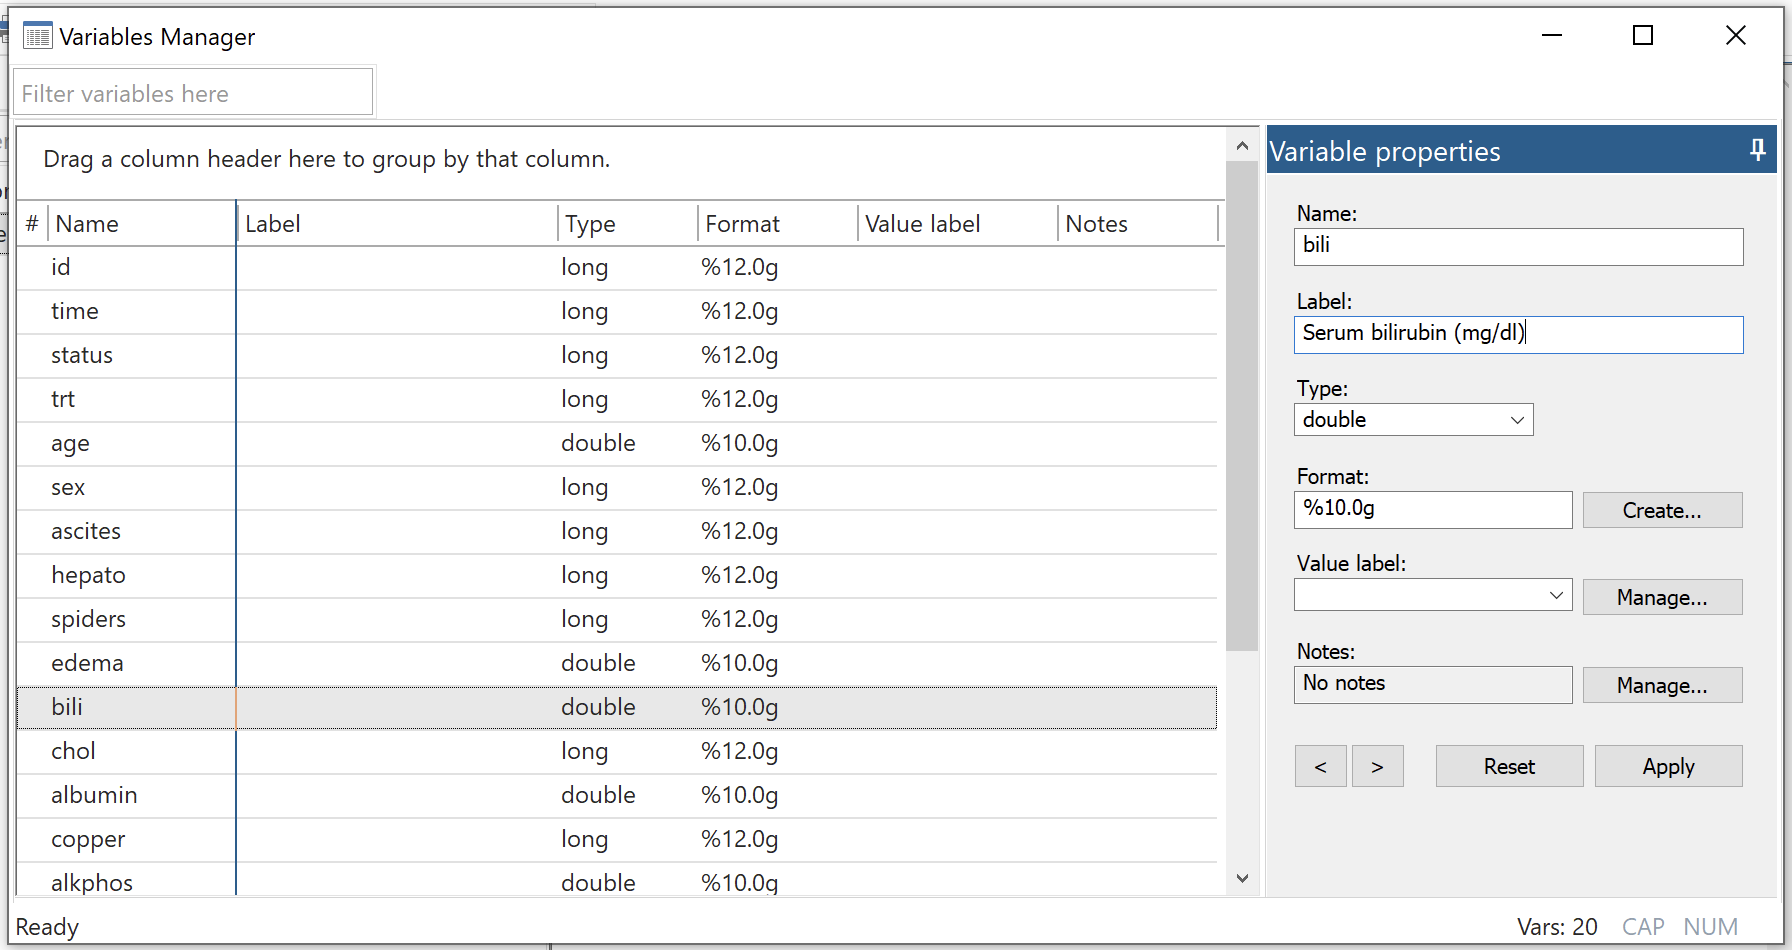
\includegraphics[width=0.75\textwidth,height=\textheight]{img/mod01/stata/label-01.png}

}

\end{figure}

The variable label will now be used in place of the variable name in
most output:

\begin{Shaded}
\begin{Highlighting}[]
\NormalTok{. summarize bili, detail}

\NormalTok{                   Serum }\FunctionTok{bilirubin}\NormalTok{ (mg}\SpecialCharTok{/}\NormalTok{dl)}
\SpecialCharTok{{-}{-}{-}{-}{-}{-}{-}{-}{-}{-}{-}{-}{-}{-}{-}{-}{-}{-}{-}{-}{-}{-}{-}{-}{-}{-}{-}{-}{-}{-}{-}{-}{-}{-}{-}{-}{-}{-}{-}{-}{-}{-}{-}{-}{-}{-}{-}{-}{-}{-}{-}{-}{-}{-}{-}{-}{-}{-}{-}{-}{-}}
\NormalTok{      Percentiles      Smallest}
 \DecValTok{1}\NormalTok{\%           .}\DecValTok{4}\NormalTok{             .}\DecValTok{3}
 \DecValTok{5}\NormalTok{\%           .}\DecValTok{5}\NormalTok{             .}\DecValTok{3}
\DecValTok{10}\NormalTok{\%           .}\DecValTok{6}\NormalTok{             .}\DecValTok{3}\NormalTok{       Obs                 }\DecValTok{418}
\DecValTok{25}\NormalTok{\%           .}\DecValTok{8}\NormalTok{             .}\DecValTok{4}\NormalTok{       Sum of Wgt.         }\DecValTok{418}

\DecValTok{50}\NormalTok{\%          }\FloatTok{1.4}\NormalTok{                      Mean           }\FloatTok{3.220813}
\NormalTok{                        Largest       Std. Dev.      }\FloatTok{4.407506}
\DecValTok{75}\NormalTok{\%          }\FloatTok{3.4}           \FloatTok{22.5}
\DecValTok{90}\NormalTok{\%          }\FloatTok{8.1}           \FloatTok{24.5}\NormalTok{       Variance       }\FloatTok{19.42611}
\DecValTok{95}\NormalTok{\%           }\DecValTok{14}           \FloatTok{25.5}\NormalTok{       Skewness       }\FloatTok{2.707849}
\DecValTok{99}\NormalTok{\%         }\FloatTok{21.6}             \DecValTok{28}\NormalTok{       Kurtosis       }\FloatTok{10.95486}
\end{Highlighting}
\end{Shaded}

\begin{tcolorbox}[enhanced jigsaw, title={TASK}, opacitybacktitle=0.6, colbacktitle=quarto-callout-note-color!10!white, titlerule=0mm, colframe=quarto-callout-note-color-frame, opacityback=0, left=2mm, breakable, bottomtitle=1mm, coltitle=black, bottomrule=.15mm, arc=.35mm, rightrule=.15mm, toptitle=1mm, colback=white, toprule=.15mm, leftrule=.75mm]

Assign meaningful variable labels to the variables used in Table 1.

\end{tcolorbox}

\hypertarget{summarising-continuous-variables}{%
\subsection{Summarising continuous
variables}\label{summarising-continuous-variables}}

As we saw in Part 1, continuous variables can be summarised using
\textbf{Statistics \textgreater{} Summaries, tables and tests
\textgreater{} Summary and descriptive statistics \textgreater{} Summary
statistics}. There are three continuous variables that we would like to
summarise: age, AST and serum bilirubin. Each of these can be listed in
the \textbf{summarize} dialog box, as shown below.

\begin{figure}[H]

{\centering 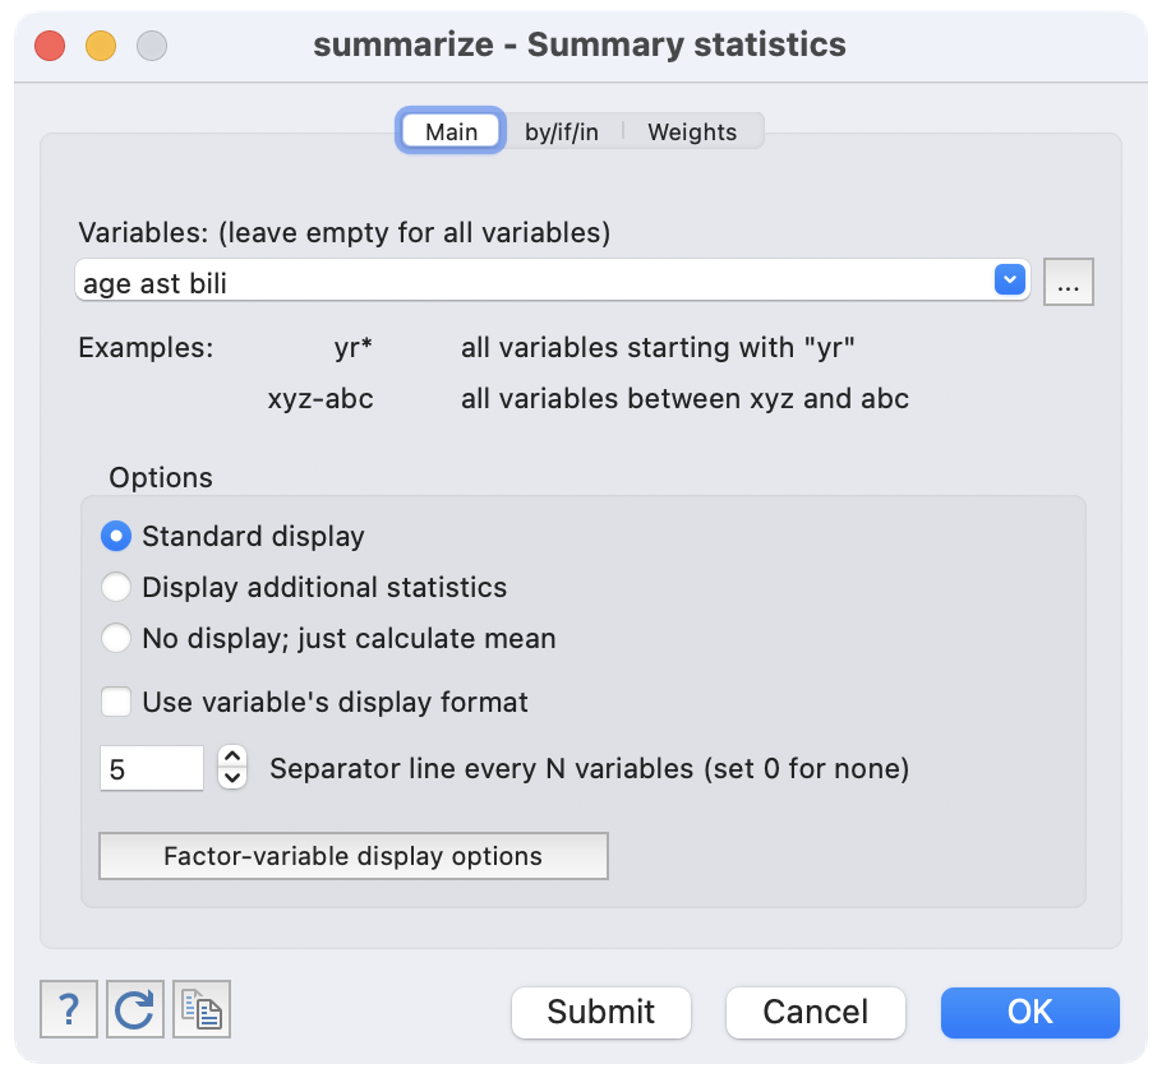
\includegraphics[width=0.75\textwidth,height=\textheight]{img/mod01/stata/summ-01.png}

}

\end{figure}

By default, the summarize command calculates the mean, standard
deviation, minimum and maximum. We may be interested in obtaining the
median and interquartile ranges, so we select the \textbf{Display
additional statistics} option:

\begin{figure}[H]

{\centering 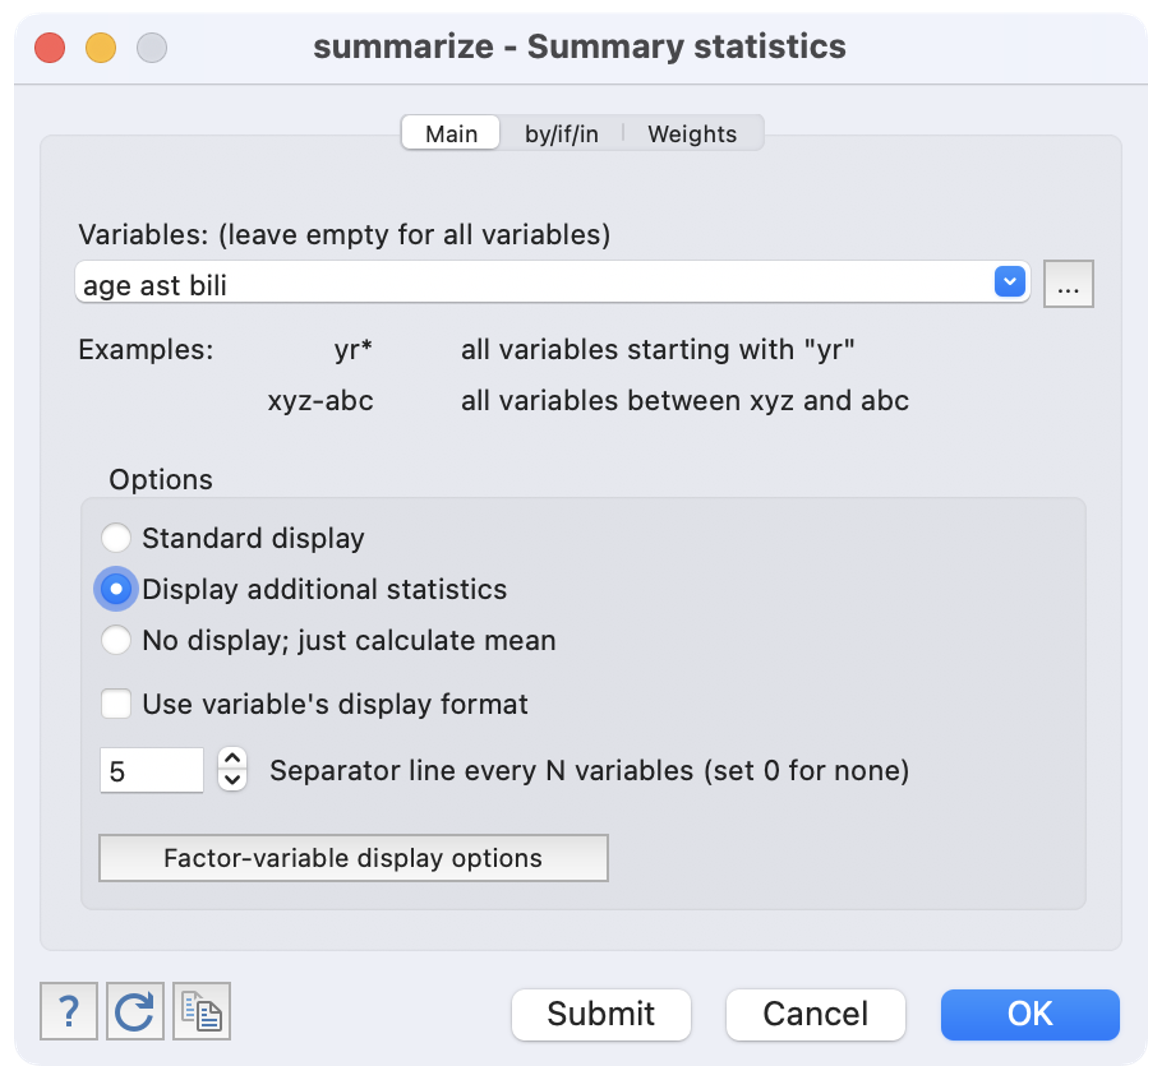
\includegraphics[width=0.75\textwidth,height=\textheight]{img/mod01/stata/summ-02.png}

}

\end{figure}

Summary statistics are produced for each of the three variables. We will
use describe the output for age:

\begin{figure}[H]

{\centering 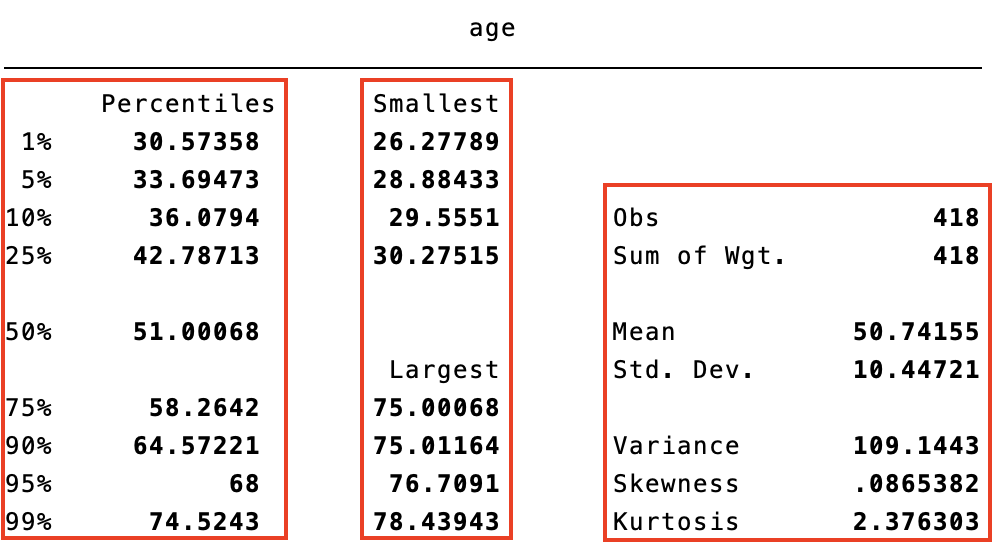
\includegraphics[width=0.75\textwidth,height=\textheight]{img/mod01/stata/summ-03.png}

}

\end{figure}

The output for a detailed summary in Stata should be read as three
separate columns. The right-most column lists the number of
observations, the mean and standard deviation and other numeric
statistics. The left-most column contains the Percentiles: median
(50\%), lower quartile (25\%) and upper quartile (75\%). The middle
column lists the four smallest and four largest observations, so that we
can assess whether the smallest and largest observations are plausible.

For each of our three continuous variables, we need to decide whether to
present the mean and standard deviation, or the median and interquartile
range. This decision can be made after examining a histogram and boxplot
for each variable.

\hypertarget{producing-a-histogram}{%
\subsection{Producing a histogram}\label{producing-a-histogram}}

To produce a histogram, go to menu \textbf{Graphics \textgreater{}
Histogram}. Choose the variable to be plotted in the \textbf{Variable}
box, and choose the \textbf{Frequency} radio button so that a frequency
histogram is produced. Note that only one variable can be plotted at a
time, so this procedure will need to be repeated for each continuous
variable.

\begin{figure}[H]

{\centering 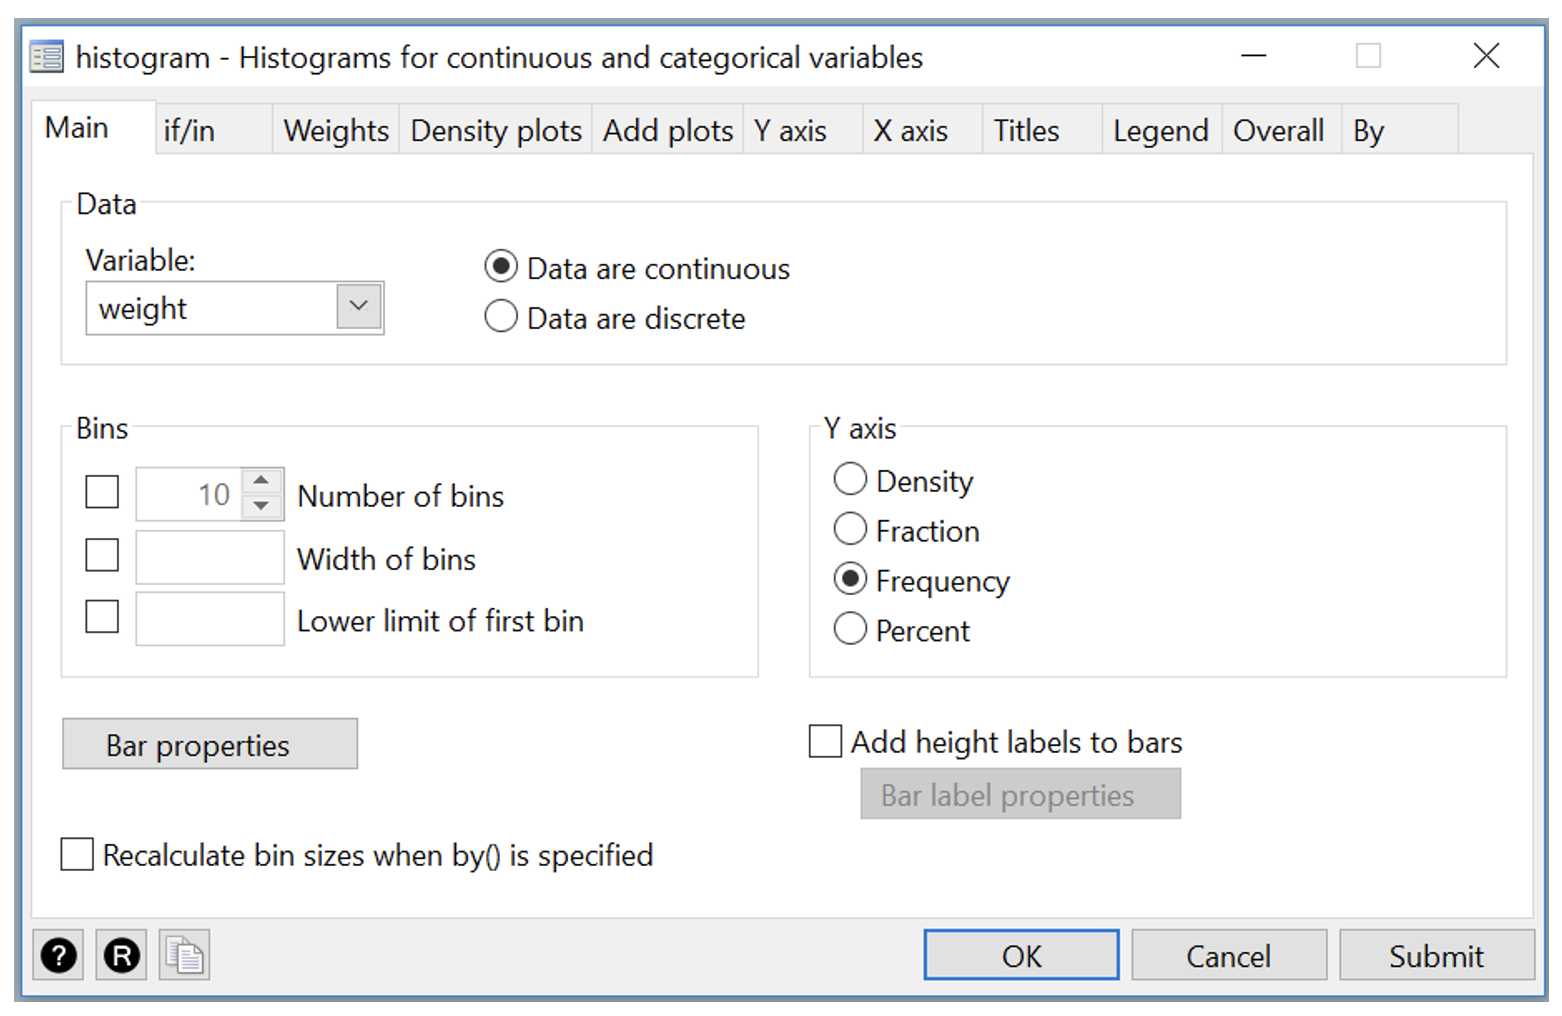
\includegraphics[width=0.75\textwidth,height=\textheight]{img/mod01/stata/hist-01.png}

}

\end{figure}

The default histogram for age appears below.

\begin{figure}[H]

{\centering 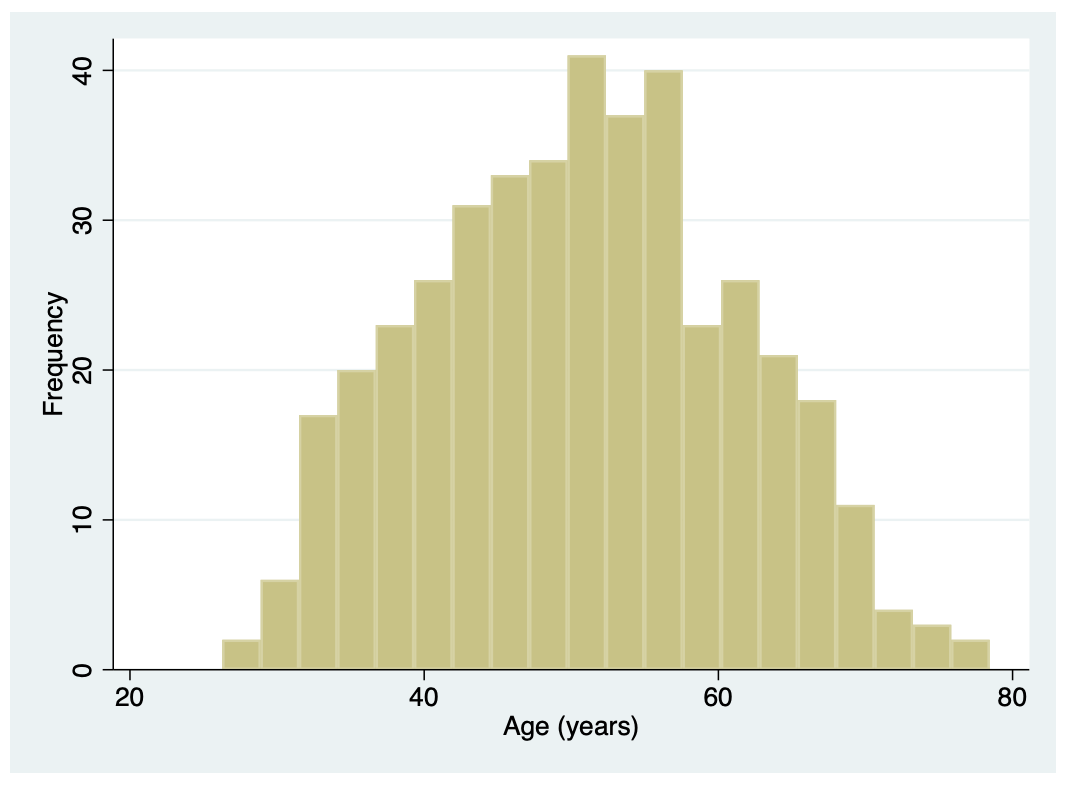
\includegraphics[width=0.75\textwidth,height=\textheight]{img/mod01/stata/hist-02.png}

}

\end{figure}

Stata will automatically choose the number of bins and the width of each
bin, however these decisions may not always produce the most optimal
histogram. These options can be altered by defining either: the number
of bins, or the bin width (but not both); and/or the lower limit of the
first bin.

Looking at the command window, Stata has used the following parameters
to define the histogram: bin=20, start=26.277892, width=2.6080767. This
means that Stata has chosen 20 bins to represent the data, with the
first bin starting at 26.2 years and each bin representing 2.6 years. A
more easily read histogram might have a bin-width of 5, starting at 25
years of age, so that age categories represent 25 to less than 30, 30 to
less than 35 etc, as defined below:

\begin{figure}[H]

{\centering 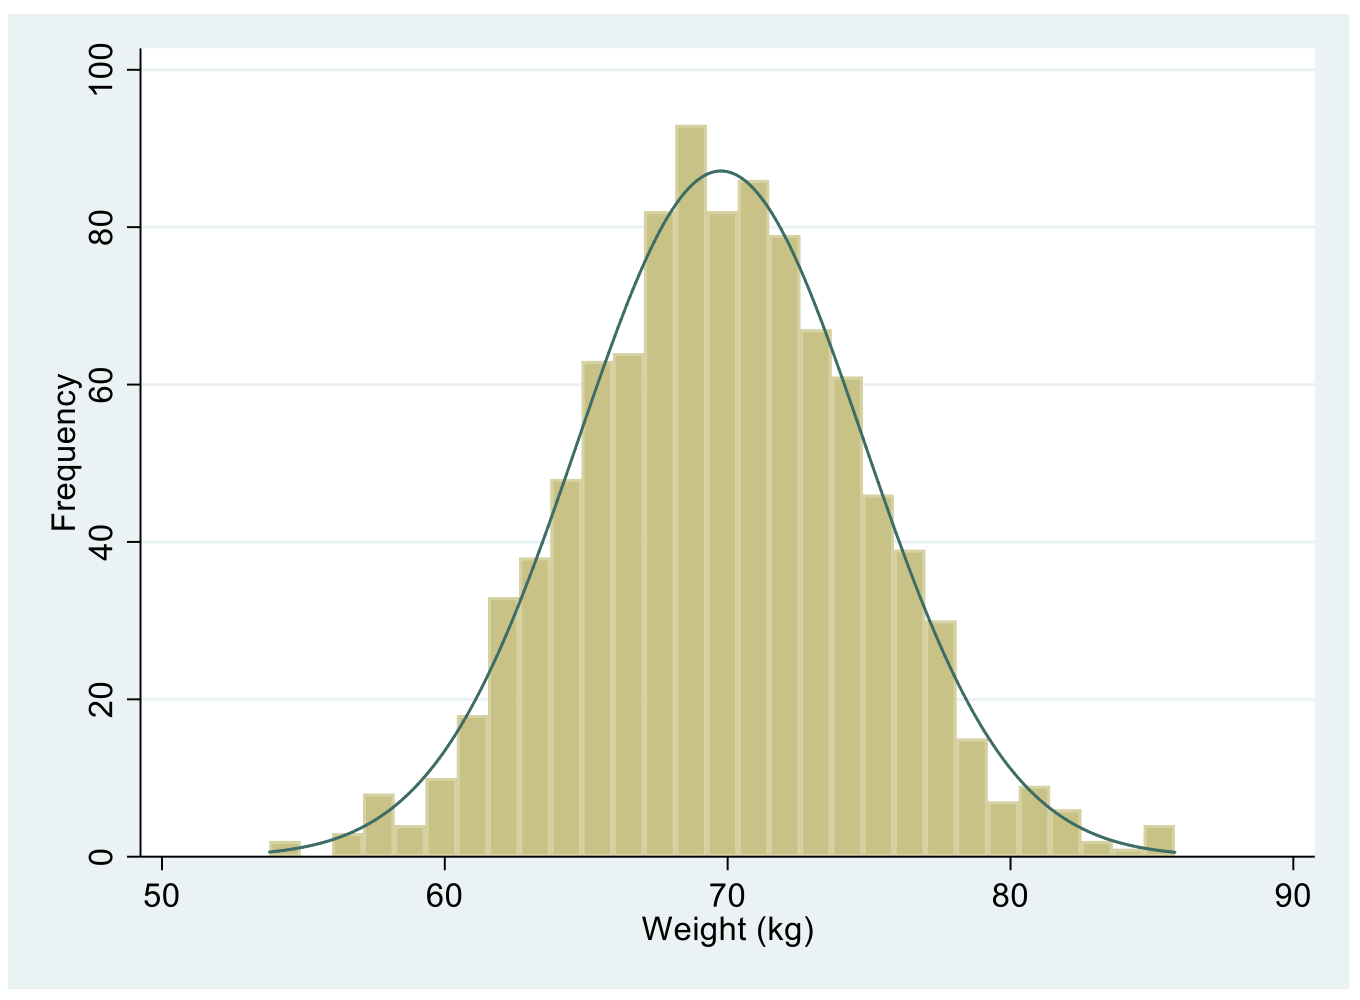
\includegraphics[width=0.75\textwidth,height=\textheight]{img/mod01/stata/hist-03.png}

}

\end{figure}

This results in a histogram with fewer bars and more sensible
cut-points:

\begin{figure}[H]

{\centering 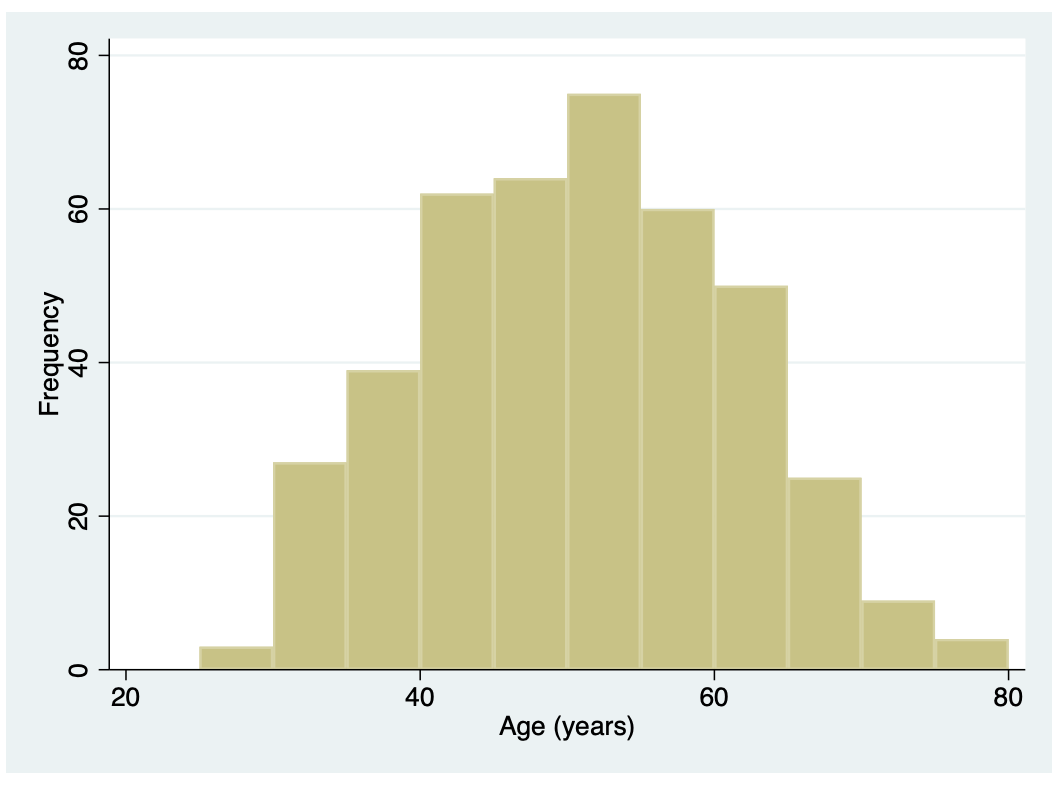
\includegraphics[width=0.75\textwidth,height=\textheight]{img/mod01/stata/hist-04.png}

}

\end{figure}

\hypertarget{producing-a-boxplot}{%
\subsection{Producing a boxplot}\label{producing-a-boxplot}}

The boxplot dialog box is similar to the histogram dialog box. While it
is possible to specify more than one variable to be plotted, this is not
recommended when variables are measured on very different scales as all
variables are plotted on a chart with the same scale.

\begin{tcolorbox}[enhanced jigsaw, title={TASK}, opacitybacktitle=0.6, colbacktitle=quarto-callout-note-color!10!white, titlerule=0mm, colframe=quarto-callout-note-color-frame, opacityback=0, left=2mm, breakable, bottomtitle=1mm, coltitle=black, bottomrule=.15mm, arc=.35mm, rightrule=.15mm, toptitle=1mm, colback=white, toprule=.15mm, leftrule=.75mm]

Obtain histograms and boxplots for age, AST and bilirubin.

Based on these plots, decide whether the mean or the median is the
appropriate summary to use for each variable.

\end{tcolorbox}

\hypertarget{producing-a-one-way-frequency-table}{%
\subsection{Producing a one-way frequency
table}\label{producing-a-one-way-frequency-table}}

We have three categorical variables to summarise in Table 1: sex, stage
and vital status. These variables are best summarised using one-way
frequency tables.

Choose \textbf{Statistics \textgreater{} Summaries, tables, and tests
\textgreater{} Frequency tables \textgreater{} One-way table}. Choose
the variable to be summarised as the \textbf{Categorical variable}, and
leave all other options unchanged:

\begin{figure}[H]

{\centering 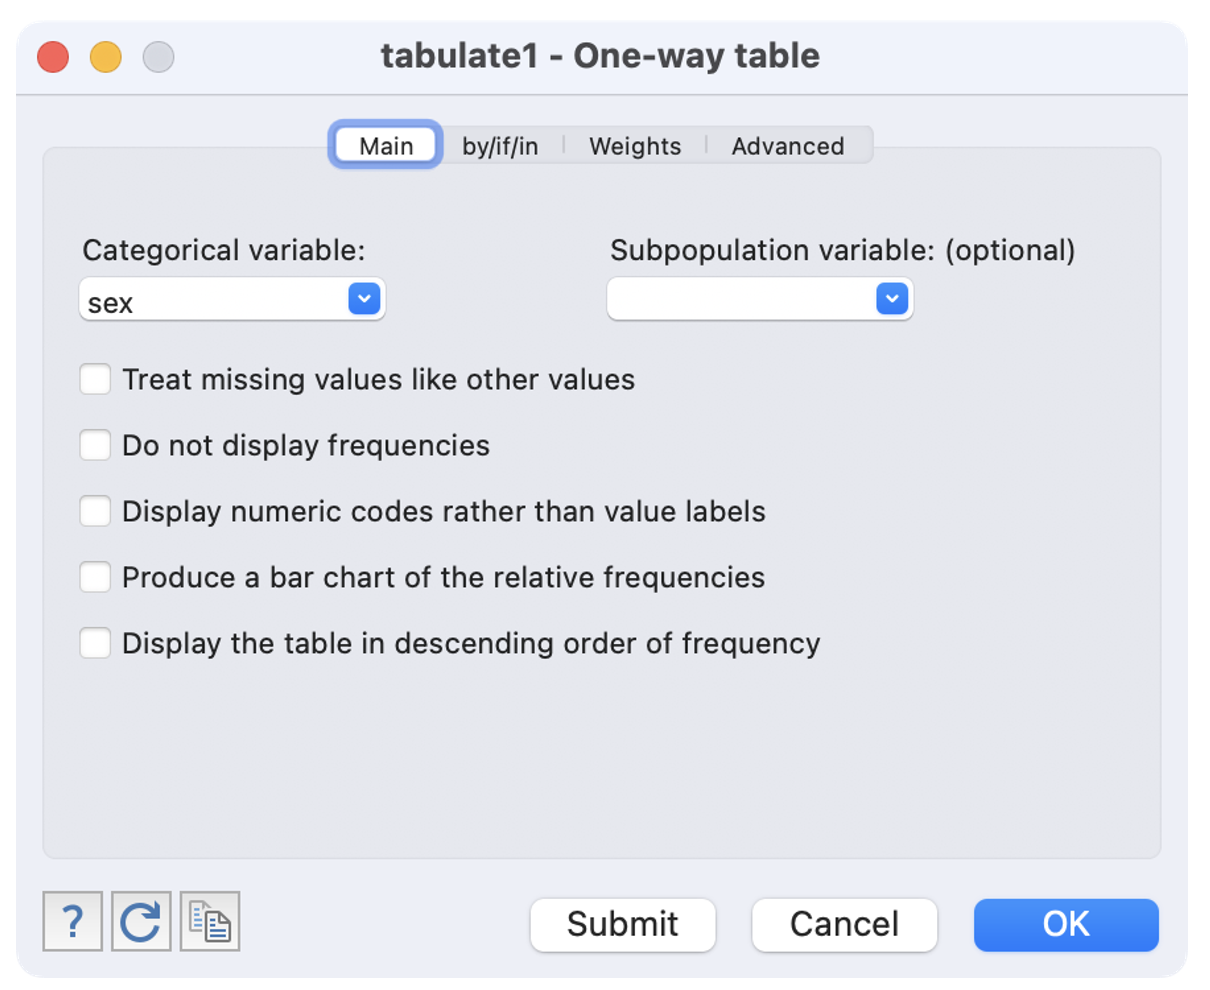
\includegraphics[width=0.75\textwidth,height=\textheight]{img/mod01/stata/tab-01.png}

}

\end{figure}

Click \textbf{OK} to obtain the following table:

\begin{Shaded}
\begin{Highlighting}[]
\NormalTok{        sex }\SpecialCharTok{|}\NormalTok{      Freq.     Percent        Cum.}
\SpecialCharTok{{-}{-}{-}{-}{-}{-}{-}{-}{-}{-}{-}{-}+{-}{-}{-}{-}{-}{-}{-}{-}{-}{-}{-}{-}{-}{-}{-}{-}{-}{-}{-}{-}{-}{-}{-}{-}{-}{-}{-}{-}{-}{-}{-}{-}{-}{-}{-}}
          \DecValTok{1} \SpecialCharTok{|}         \DecValTok{44}       \FloatTok{10.53}       \FloatTok{10.53}
          \DecValTok{2} \SpecialCharTok{|}        \DecValTok{374}       \FloatTok{89.47}      \FloatTok{100.00}
\SpecialCharTok{{-}{-}{-}{-}{-}{-}{-}{-}{-}{-}{-}{-}+{-}{-}{-}{-}{-}{-}{-}{-}{-}{-}{-}{-}{-}{-}{-}{-}{-}{-}{-}{-}{-}{-}{-}{-}{-}{-}{-}{-}{-}{-}{-}{-}{-}{-}{-}}
\NormalTok{      Total }\SpecialCharTok{|}        \DecValTok{418}      \FloatTok{100.00}
\end{Highlighting}
\end{Shaded}

\hypertarget{assigning-value-labels-to-categorical-variables}{%
\subsection{Assigning value labels to categorical
variables}\label{assigning-value-labels-to-categorical-variables}}

You will notice that the table above, in its current form, is
uninterpretable as the 1 and 2 categories are not labelled. In this
course, all variables including categorical variables are numerically
coded. This is because ``string'' or ``character'' variables
(e.g.~entered as ``male'' or ``female'') cannot be used in many of the
analysis commands of Stata. Instead, we use numerical codes and assign
labels to the categories.

There are two parts to applying value labels to categorical variables:
1) defining the labels, and 2) applying the labels to a variable. This
may seem cumbersome, but there are times where we can apply value labels
to a collection of variables (for example, multiple variables comprising
yes/no categories, or Likert scales such as: strongly disagree,
disagree, neutral, agree, strongly agree). Both parts can be done within
the Variables Manager.

\textbf{Part 1:} Defining the value labels

\begin{enumerate}
\def\labelenumi{\arabic{enumi}.}
\tightlist
\item
  Open the Variables Manager: \textbf{Data \textgreater{} Variables
  Manager} and select the variable you want to assign labels to (in this
  case, \texttt{sex}). You will see that the \textbf{Value label} in the
  \textbf{Properties} section is blank. To create a value label, click
  \textbf{Manage}.
\end{enumerate}

Alternatively, choose \textbf{Data \textgreater{} Data utilities
\textgreater{} Label utilities \textgreater{} Manage value labels}.

\begin{figure}[H]

{\centering 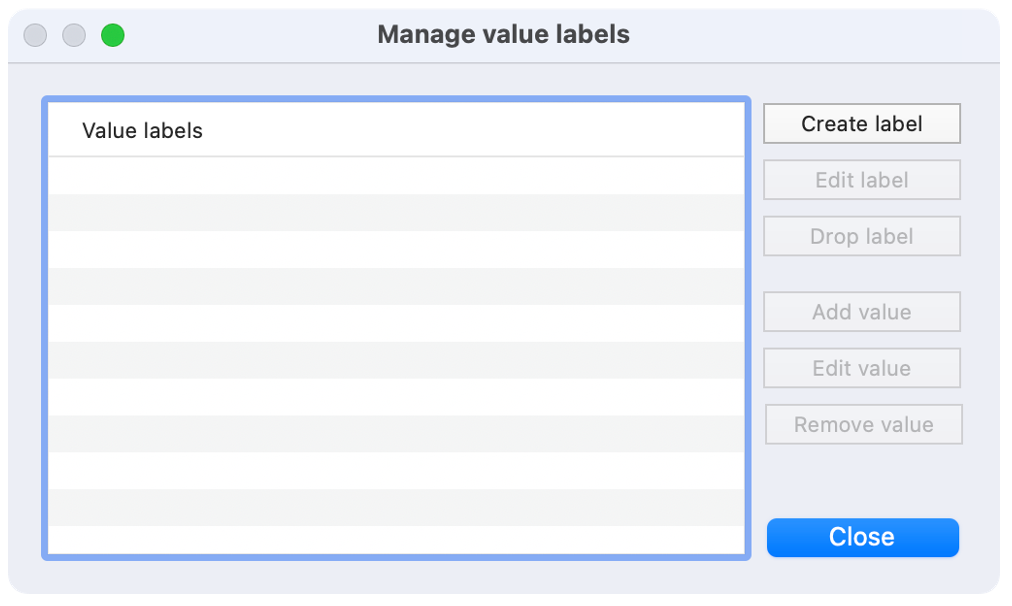
\includegraphics[width=0.75\textwidth,height=\textheight]{img/mod01/stata/value-labels-01.png}

}

\end{figure}

In the \textbf{Manage value labels} dialog box, click the \textbf{Create
label} button.

\begin{enumerate}
\def\labelenumi{\arabic{enumi}.}
\setcounter{enumi}{1}
\item
  In the next dialog box, enter a name for the value label such as
  \texttt{sex\_label} in the \textbf{Label name:} box. You can use the
  same name of the variable for the label, or choose a different name.
  Note: as for variables, the value label name is case-sensitive.
\item
  Next, we specify what each category (i.e.~1 and 2) represents. By
  checking the metadata document, we see that \texttt{1} represents
  ``Male'' and \texttt{2} represents ``Female''. Type the number
  \texttt{1} in the \textbf{Value:} box and the word \texttt{Male} in
  the \textbf{Label:} box; then click the \textbf{Add} button. Then type
  the number \texttt{2} in the \textbf{Value:} box and the word
  \texttt{Female} in the \textbf{Label:} box; click the \textbf{Add}
  button again. The defined value labels for males and females should
  appear in the box on the left-hand side. When you are done, click the
  \textbf{OK} button.
\end{enumerate}

\begin{figure}[H]

{\centering 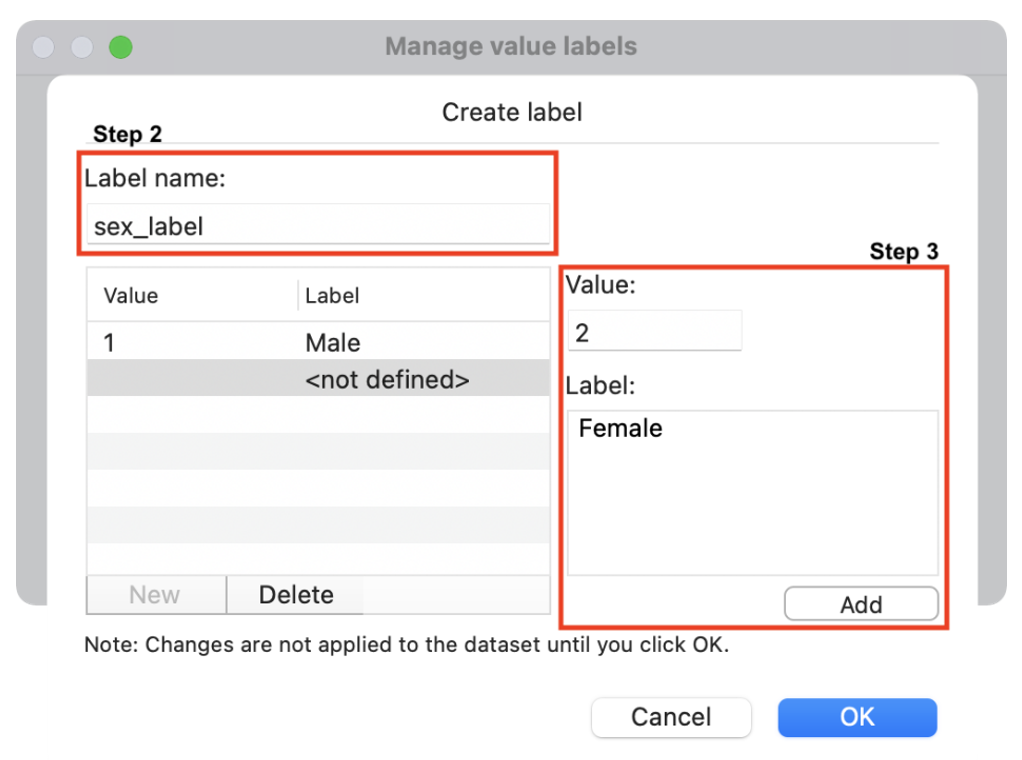
\includegraphics[width=0.75\textwidth,height=\textheight]{img/mod01/stata/value-labels-02.png}

}

\end{figure}

You will be returned to the \textbf{Manage value labels} dialog box,
which will now have a record for \texttt{sex\_label}. By clicking the
arrow next to the label name, you will see the codes that you have
defined:

\begin{figure}[H]

{\centering 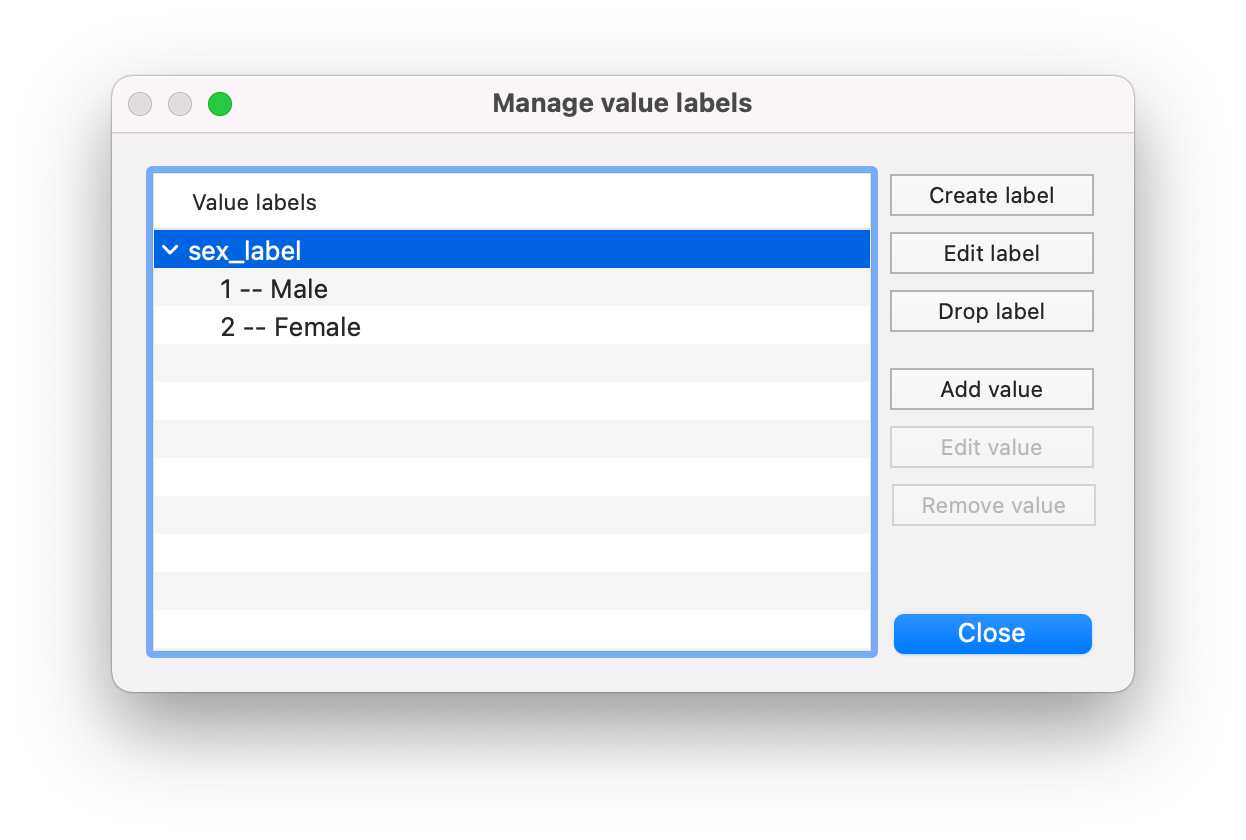
\includegraphics[width=0.75\textwidth,height=\textheight]{img/mod01/stata/value-labels-03.png}

}

\end{figure}

At this point, you can close the \textbf{Manage value labels} dialog box
by clicking \textbf{Close}.

\textbf{Part 2:} Applying the value labels to a variable

Now that the labels are defined, we need to attach them to the relevant
variables. Within the Variables Manager, click the variable to be
labelled (here, \texttt{sex}). The previously defined label can be
assigned to this variable by clicking the \textbf{Value label} drop-down
menu, and choosing the appropriate label (here, \texttt{sex\_label}),
and clicking \textbf{Apply}:

\begin{figure}[H]

{\centering 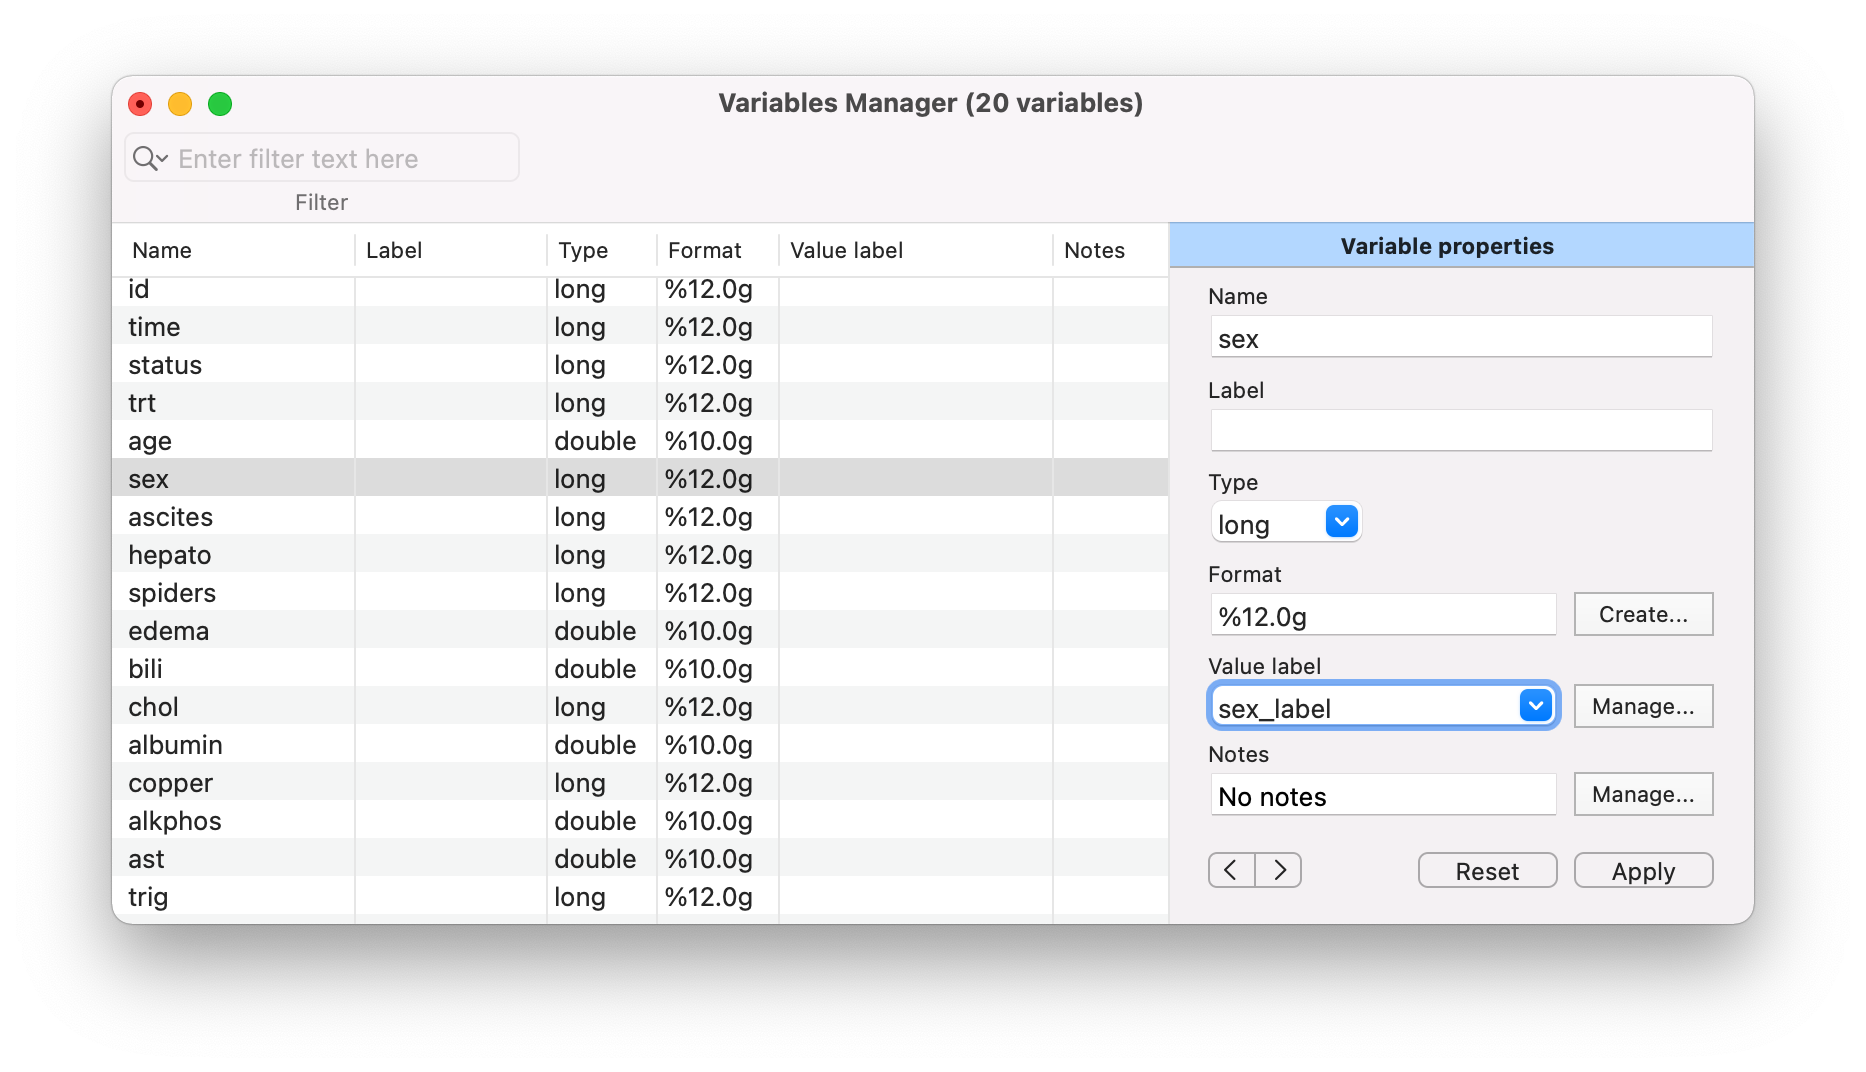
\includegraphics[width=0.75\textwidth,height=\textheight]{img/mod01/stata/value-labels-04-1.png}

}

\end{figure}

Alternatively, go to \textbf{Data \textgreater{} Data utilities
\textgreater{} Label utilities \textgreater{} Assign value label to
variables}. Select \texttt{sex} from the \textbf{Variables:} dropdown
box, and select \texttt{sex\_label} from the \textbf{Value label:}
dropdown box. Click \textbf{OK}.

\begin{figure}[H]

{\centering 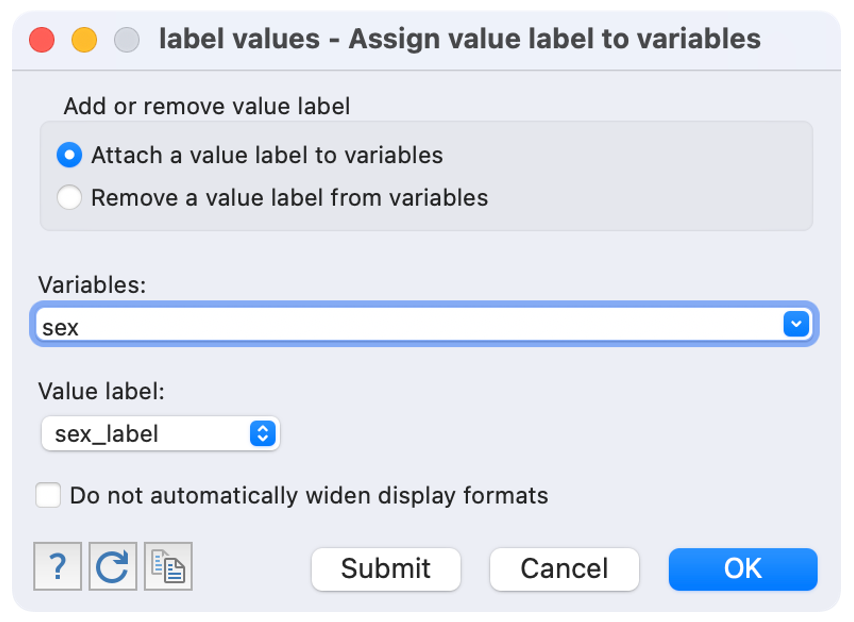
\includegraphics[width=0.75\textwidth,height=\textheight]{img/mod01/stata/value-labels-04.png}

}

\end{figure}

There are a number of ways that we can confirm that the labelling has
been done correctly. One of the easiest ways is to use the
\texttt{codebook} command to investigate the coding of sex: \textbf{Data
\textgreater{} Describe data \textgreater{} Describe data contents
(codebook)}.

\begin{Shaded}
\begin{Highlighting}[]
\NormalTok{. codebook sex}

\SpecialCharTok{{-}{-}{-}{-}{-}{-}{-}{-}{-}{-}{-}{-}{-}{-}{-}{-}{-}{-}{-}{-}{-}{-}{-}{-}{-}{-}{-}{-}{-}{-}{-}{-}{-}{-}{-}{-}{-}{-}{-}{-}{-}{-}{-}{-}{-}{-}{-}{-}{-}{-}{-}{-}{-}{-}{-}{-}{-}{-}{-}{-}{-}{-}{-}{-}{-}{-}{-}{-}{-}{-}{-}{-}{-}{-}{-}{-}{-}{-}{-}{-}{-}{-}{-}{-}{-}{-}{-}{-}}
\FunctionTok{sex}\NormalTok{                                                                          (unlabeled)}
\SpecialCharTok{{-}{-}{-}{-}{-}{-}{-}{-}{-}{-}{-}{-}{-}{-}{-}{-}{-}{-}{-}{-}{-}{-}{-}{-}{-}{-}{-}{-}{-}{-}{-}{-}{-}{-}{-}{-}{-}{-}{-}{-}{-}{-}{-}{-}{-}{-}{-}{-}{-}{-}{-}{-}{-}{-}{-}{-}{-}{-}{-}{-}{-}{-}{-}{-}{-}{-}{-}{-}{-}{-}{-}{-}{-}{-}{-}{-}{-}{-}{-}{-}{-}{-}{-}{-}{-}{-}{-}{-}}

\NormalTok{                  type}\SpecialCharTok{:}  \FunctionTok{numeric}\NormalTok{ (long)}
\NormalTok{                 label}\SpecialCharTok{:}\NormalTok{  sex\_label}

\NormalTok{                 range}\SpecialCharTok{:}\NormalTok{  [}\DecValTok{1}\NormalTok{,}\DecValTok{2}\NormalTok{]                        units}\SpecialCharTok{:}  \DecValTok{1}
\NormalTok{         unique values}\SpecialCharTok{:}  \DecValTok{2}\NormalTok{                        missing .}\SpecialCharTok{:}  \DecValTok{0}\SpecialCharTok{/}\DecValTok{418}

\NormalTok{            tabulation}\SpecialCharTok{:}\NormalTok{  Freq.   Numeric  Label}
                            \DecValTok{44}         \DecValTok{1}\NormalTok{  Male}
                           \DecValTok{374}         \DecValTok{2}\NormalTok{  Female}
\end{Highlighting}
\end{Shaded}

Here we can see that the codes for male and female have been applied
correctly. We can also examine the Data Browser and confirm that sex has
been labelled.

Note: If you want to see the original coded values of the labelled
groups in the Data Browser window, you can hide the value labels by
choosing \textbf{Tools \textgreater{} Value labels \textgreater{} Hide
all value labels} for Windows, or \textbf{View \textgreater{} Value
labels \textgreater{} Hide all value labels} for Mac from the menu bar
in the Data Browser window.

Now that our categorical variables are labelled, we can produce the
one-way frequency tables. As before, choose \textbf{Statistics
\textgreater{} Summaries, tables, and tests \textgreater{} Frequency
tables \textgreater{} One-way table}. Our newly labelled table for sex
appears as below.

\begin{Shaded}
\begin{Highlighting}[]
\NormalTok{        sex }\SpecialCharTok{|}\NormalTok{      Freq.     Percent        Cum.}
\SpecialCharTok{{-}{-}{-}{-}{-}{-}{-}{-}{-}{-}{-}{-}+{-}{-}{-}{-}{-}{-}{-}{-}{-}{-}{-}{-}{-}{-}{-}{-}{-}{-}{-}{-}{-}{-}{-}{-}{-}{-}{-}{-}{-}{-}{-}{-}{-}{-}{-}}
\NormalTok{       Male }\SpecialCharTok{|}         \DecValTok{44}       \FloatTok{10.53}       \FloatTok{10.53}
\NormalTok{     Female }\SpecialCharTok{|}        \DecValTok{374}       \FloatTok{89.47}      \FloatTok{100.00}
\SpecialCharTok{{-}{-}{-}{-}{-}{-}{-}{-}{-}{-}{-}{-}+{-}{-}{-}{-}{-}{-}{-}{-}{-}{-}{-}{-}{-}{-}{-}{-}{-}{-}{-}{-}{-}{-}{-}{-}{-}{-}{-}{-}{-}{-}{-}{-}{-}{-}{-}}
\NormalTok{      Total }\SpecialCharTok{|}        \DecValTok{418}      \FloatTok{100.00}
\end{Highlighting}
\end{Shaded}

\begin{tcolorbox}[enhanced jigsaw, title={TASK}, opacitybacktitle=0.6, colbacktitle=quarto-callout-note-color!10!white, titlerule=0mm, colframe=quarto-callout-note-color-frame, opacityback=0, left=2mm, breakable, bottomtitle=1mm, coltitle=black, bottomrule=.15mm, arc=.35mm, rightrule=.15mm, toptitle=1mm, colback=white, toprule=.15mm, leftrule=.75mm]

Create and apply value labels for Sex and Vital Status. Produce one-way
frequency tables for the categorical variables in Table 1.

\end{tcolorbox}

\hypertarget{producing-a-two-way-frequency-table}{%
\subsection{Producing a two-way frequency
table}\label{producing-a-two-way-frequency-table}}

To produce tables summarising two categorical variables, go to
\textbf{Statistics - Summaries, tables, and tests - Frequency tables -
Two-way table with measures of association}.

To produce a two-way table showing stage of disease by sex using the
mod01\_pbc.dta data, do the following. In the \textbf{tabulate2 -- two
way table with measures of association dialog box}, select the variable
\texttt{sex} as the \textbf{Row variable:}, and \texttt{stage} as the
\textbf{Column variable:} as shown below.

\begin{figure}[H]

{\centering 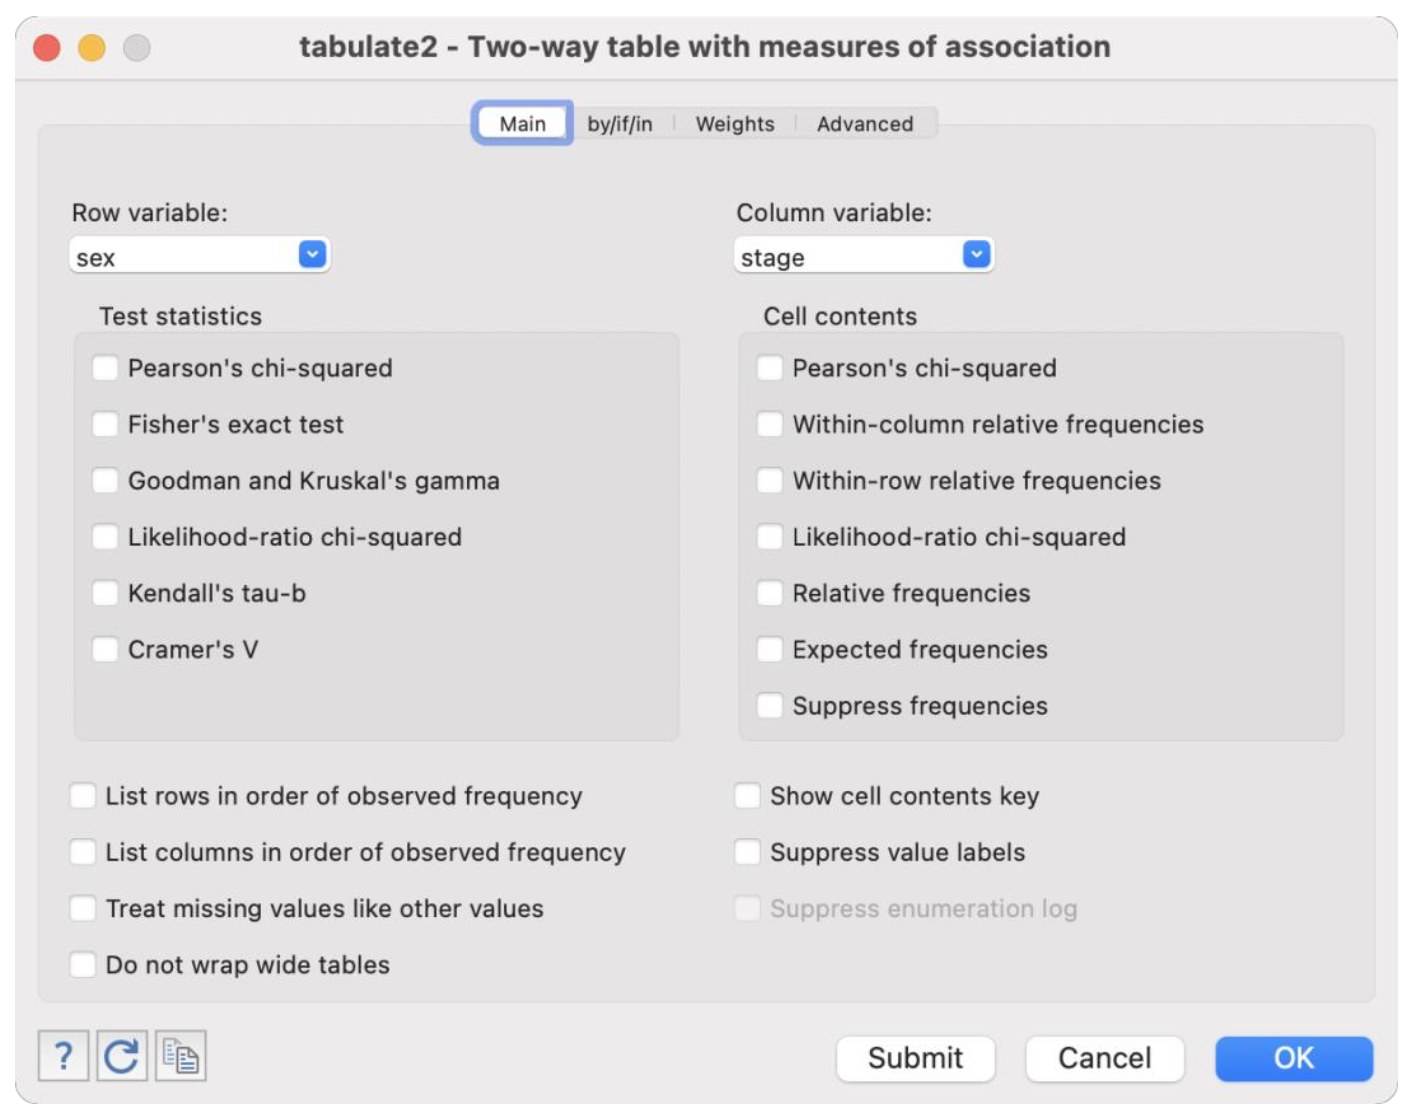
\includegraphics[width=0.75\textwidth,height=\textheight]{img/mod01/stata/mod01-twoway.png}

}

\end{figure}

Click \textbf{OK} to obtain the output below.

\begin{Shaded}
\begin{Highlighting}[]
\NormalTok{. tabulate sex stage}

           \SpecialCharTok{|}\NormalTok{                    stage}
\NormalTok{       sex }\SpecialCharTok{|}\NormalTok{   Stage }\DecValTok{1}\NormalTok{    Stage }\DecValTok{2}\NormalTok{    Stage }\DecValTok{3}\NormalTok{    Stage }\DecValTok{4} \SpecialCharTok{|}\NormalTok{     Total}
\SpecialCharTok{{-}{-}{-}{-}{-}{-}{-}{-}{-}{-}{-}+{-}{-}{-}{-}{-}{-}{-}{-}{-}{-}{-}{-}{-}{-}{-}{-}{-}{-}{-}{-}{-}{-}{-}{-}{-}{-}{-}{-}{-}{-}{-}{-}{-}{-}{-}{-}{-}{-}{-}{-}{-}{-}{-}{-}+{-}{-}{-}{-}{-}{-}{-}{-}{-}{-}}
\NormalTok{      Male }\SpecialCharTok{|}         \DecValTok{3}          \DecValTok{8}         \DecValTok{16}         \DecValTok{17} \SpecialCharTok{|}        \DecValTok{44} 
\NormalTok{    Female }\SpecialCharTok{|}        \DecValTok{18}         \DecValTok{84}        \DecValTok{139}        \DecValTok{127} \SpecialCharTok{|}       \DecValTok{368} 
\SpecialCharTok{{-}{-}{-}{-}{-}{-}{-}{-}{-}{-}{-}+{-}{-}{-}{-}{-}{-}{-}{-}{-}{-}{-}{-}{-}{-}{-}{-}{-}{-}{-}{-}{-}{-}{-}{-}{-}{-}{-}{-}{-}{-}{-}{-}{-}{-}{-}{-}{-}{-}{-}{-}{-}{-}{-}{-}+{-}{-}{-}{-}{-}{-}{-}{-}{-}{-}}
\NormalTok{     Total }\SpecialCharTok{|}        \DecValTok{21}         \DecValTok{92}        \DecValTok{155}        \DecValTok{144} \SpecialCharTok{|}       \DecValTok{412} 
\end{Highlighting}
\end{Shaded}

You may notice in the above that the number of observations is now 412.
This is because there are missing observations for either sex or stage:
which is it, and how would you determine this?

From the cross-tabulation, you can see the individual frequencies of
participants in each of the categories in each cell. For example, there
are 3 male participants who have Stage 1 disease. You can also read the
totals for each row and column. For example, there are 44 males, and 144
participants have Stage 4 disease.

You can also add percentages into your table. For example, in the
\textbf{tabulate2 -- two way table with measures of association} dialog
box tick the box \textbf{Within-column relative frequencies} for
separate percentages of sex within each stage.

\begin{Shaded}
\begin{Highlighting}[]
\NormalTok{. tabulate sex stage, column}

\SpecialCharTok{+{-}{-}{-}{-}{-}{-}{-}{-}{-}{-}{-}{-}{-}{-}{-}{-}{-}{-}{-}+}
\ErrorTok{|}\NormalTok{ Key               }\SpecialCharTok{|}
\ErrorTok{|}\SpecialCharTok{{-}{-}{-}{-}{-}{-}{-}{-}{-}{-}{-}{-}{-}{-}{-}{-}{-}{-}{-}}\ErrorTok{|}
\ErrorTok{|}\NormalTok{     frequency     }\SpecialCharTok{|}
\ErrorTok{|}\NormalTok{ column percentage }\SpecialCharTok{|}
\SpecialCharTok{+{-}{-}{-}{-}{-}{-}{-}{-}{-}{-}{-}{-}{-}{-}{-}{-}{-}{-}{-}+}

           \ErrorTok{|}\NormalTok{                    stage}
\NormalTok{       sex }\SpecialCharTok{|}\NormalTok{   Stage }\DecValTok{1}\NormalTok{    Stage }\DecValTok{2}\NormalTok{    Stage }\DecValTok{3}\NormalTok{    Stage }\DecValTok{4} \SpecialCharTok{|}\NormalTok{     Total}
\SpecialCharTok{{-}{-}{-}{-}{-}{-}{-}{-}{-}{-}{-}+{-}{-}{-}{-}{-}{-}{-}{-}{-}{-}{-}{-}{-}{-}{-}{-}{-}{-}{-}{-}{-}{-}{-}{-}{-}{-}{-}{-}{-}{-}{-}{-}{-}{-}{-}{-}{-}{-}{-}{-}{-}{-}{-}{-}+{-}{-}{-}{-}{-}{-}{-}{-}{-}{-}}
\NormalTok{      Male }\SpecialCharTok{|}         \DecValTok{3}          \DecValTok{8}         \DecValTok{16}         \DecValTok{17} \SpecialCharTok{|}        \DecValTok{44} 
           \SpecialCharTok{|}     \FloatTok{14.29}       \FloatTok{8.70}      \FloatTok{10.32}      \FloatTok{11.81} \SpecialCharTok{|}     \FloatTok{10.68} 
\SpecialCharTok{{-}{-}{-}{-}{-}{-}{-}{-}{-}{-}{-}+{-}{-}{-}{-}{-}{-}{-}{-}{-}{-}{-}{-}{-}{-}{-}{-}{-}{-}{-}{-}{-}{-}{-}{-}{-}{-}{-}{-}{-}{-}{-}{-}{-}{-}{-}{-}{-}{-}{-}{-}{-}{-}{-}{-}+{-}{-}{-}{-}{-}{-}{-}{-}{-}{-}}
\NormalTok{    Female }\SpecialCharTok{|}        \DecValTok{18}         \DecValTok{84}        \DecValTok{139}        \DecValTok{127} \SpecialCharTok{|}       \DecValTok{368} 
           \SpecialCharTok{|}     \FloatTok{85.71}      \FloatTok{91.30}      \FloatTok{89.68}      \FloatTok{88.19} \SpecialCharTok{|}     \FloatTok{89.32} 
\SpecialCharTok{{-}{-}{-}{-}{-}{-}{-}{-}{-}{-}{-}+{-}{-}{-}{-}{-}{-}{-}{-}{-}{-}{-}{-}{-}{-}{-}{-}{-}{-}{-}{-}{-}{-}{-}{-}{-}{-}{-}{-}{-}{-}{-}{-}{-}{-}{-}{-}{-}{-}{-}{-}{-}{-}{-}{-}+{-}{-}{-}{-}{-}{-}{-}{-}{-}{-}}
\NormalTok{     Total }\SpecialCharTok{|}        \DecValTok{21}         \DecValTok{92}        \DecValTok{155}        \DecValTok{144} \SpecialCharTok{|}       \DecValTok{412} 
           \SpecialCharTok{|}    \FloatTok{100.00}     \FloatTok{100.00}     \FloatTok{100.00}     \FloatTok{100.00} \SpecialCharTok{|}    \FloatTok{100.00} 
\end{Highlighting}
\end{Shaded}

We can see that the 3 male participants with Stage 1 disease made up
14\% of those with Stage 1 disease.

\hypertarget{saving-data-from-stata}{%
\subsection{Saving data from Stata}\label{saving-data-from-stata}}

Now that you have made some changes to the pbc data, it is good practice
to save the dataset. Stata uses its own file format to save data. Data
saved from Stata will end with the .dta suffix, and will contain useful
information such as variable labels and value labels, as well as any new
variables created. However, data saved by Stata will only be able to be
opened by Stata - you will not easily be able to share your data with
colleagues who do not have Stata. To save a Stata dataset, choose
\textbf{File \textgreater{} Save}.

If you want to share data with colleagues who do not have Stata, you can
use \textbf{File \textgreater{} Export} to save your data in another
file format (recognising that variable and value labels will not be
exported.)

\hypertarget{copying-output-from-stata}{%
\subsection{Copying output from Stata}\label{copying-output-from-stata}}

It is important to note that \emph{saving data in Stata will not save
your output}. Stata data and output are completely separate to one
another. The easiest way to retain the output of your analyses is to
copy the output into a word processor package (e.g.~Microsoft Word)
before closing Stata. Once Stata is closed, all the output (that is, all
your hard work!) is lost.

To copy output from Stata, you can select the output and choose
\textbf{Edit \textgreater{} Copy}. This will copy the output as plain
text for pasting into a Word document. If you select a single table for
copying, you can also \textbf{Copy table} or \textbf{Copy table as
HTML}. Whichever way you copy output into Word, you will need to make
sure you reformat the table and relabel your header row and column
properly for your assignments as described in Module 1. Alternatively,
you can copy with the Copy table option for pasting into an Excel
worksheet and reformat your table in Excel before pasting into Word.

\begin{tcolorbox}[enhanced jigsaw, title={TASK}, opacitybacktitle=0.6, colbacktitle=quarto-callout-note-color!10!white, titlerule=0mm, colframe=quarto-callout-note-color-frame, opacityback=0, left=2mm, breakable, bottomtitle=1mm, coltitle=black, bottomrule=.15mm, arc=.35mm, rightrule=.15mm, toptitle=1mm, colback=white, toprule=.15mm, leftrule=.75mm]

Complete Table 1 using the output generated in this exercise. You should
decide on whether to present continuous variables by their means or
medians, and present the most appropriate measure of spread. Include
footnotes to indicate if any variables contain missing observations.

\end{tcolorbox}

\hypertarget{part-3-creating-other-types-of-graphs}{%
\section{Part 3: Creating other types of
graphs}\label{part-3-creating-other-types-of-graphs}}

\hypertarget{bar-graphs}{%
\subsection{Bar graphs}\label{bar-graphs}}

Here we will create the bar chart shown in Figure~\ref{fig-bar-1} using
the \texttt{mod01\_pbc.dta} dataset. The x-axis of this graph will be
the stage of disease, and the y-axis will show the number of
participants in each category.

To create a Bar chart, go to the Stata menu Graphics \textgreater{} Bar
chart and the bar-chart dialog box will appear.

\hypertarget{simple-bar-graph}{%
\subsubsection{Simple bar graph}\label{simple-bar-graph}}

For most of our bar graphs, we will be plotting frequencies, so we
choose \textbf{Graph of frequencies within categories}

\begin{figure}[H]

{\centering 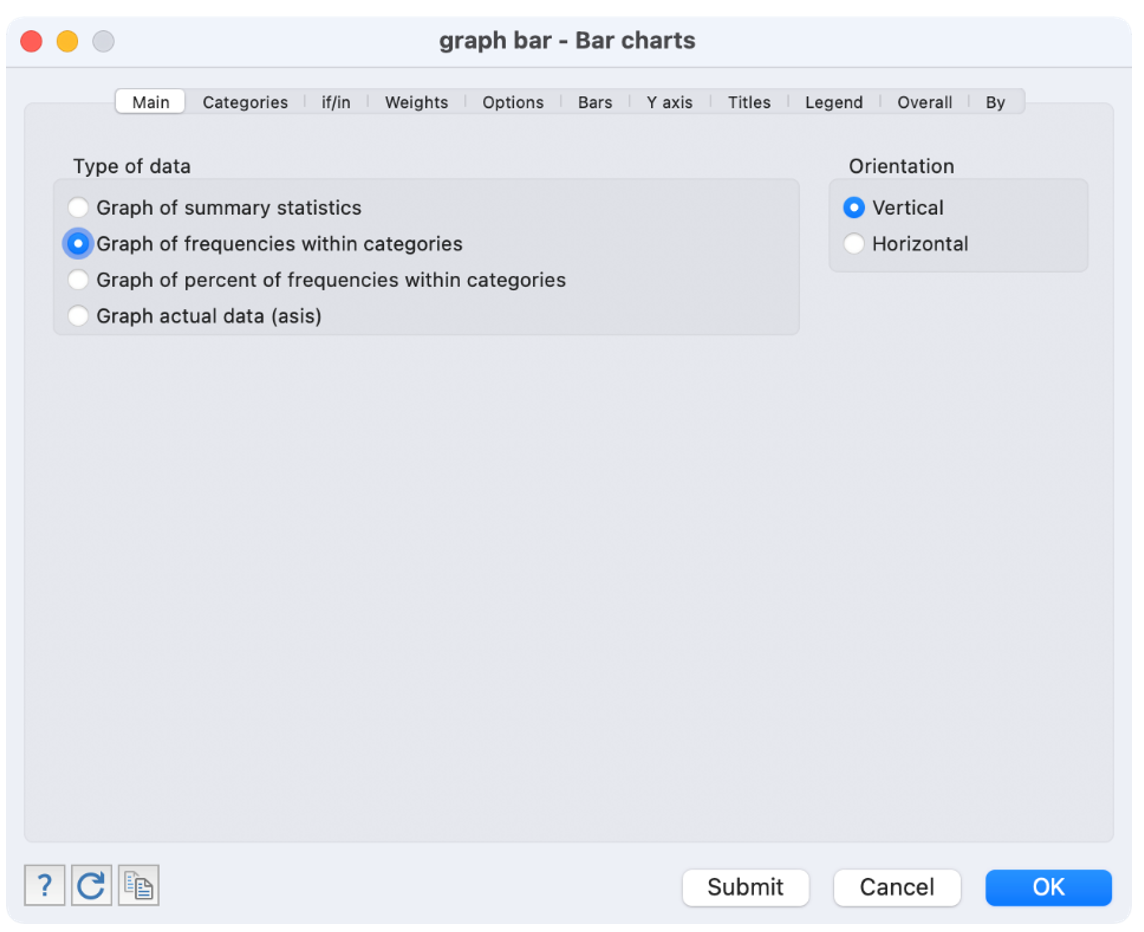
\includegraphics[width=0.75\textwidth,height=\textheight]{img/mod01/stata/bar-01.png}

}

\end{figure}

For a simple bar graph, go to the \textbf{Categories} tab, tick the
\textbf{Group 1} box and choose \texttt{stage} as your first grouping
variable:

\begin{figure}[H]

{\centering 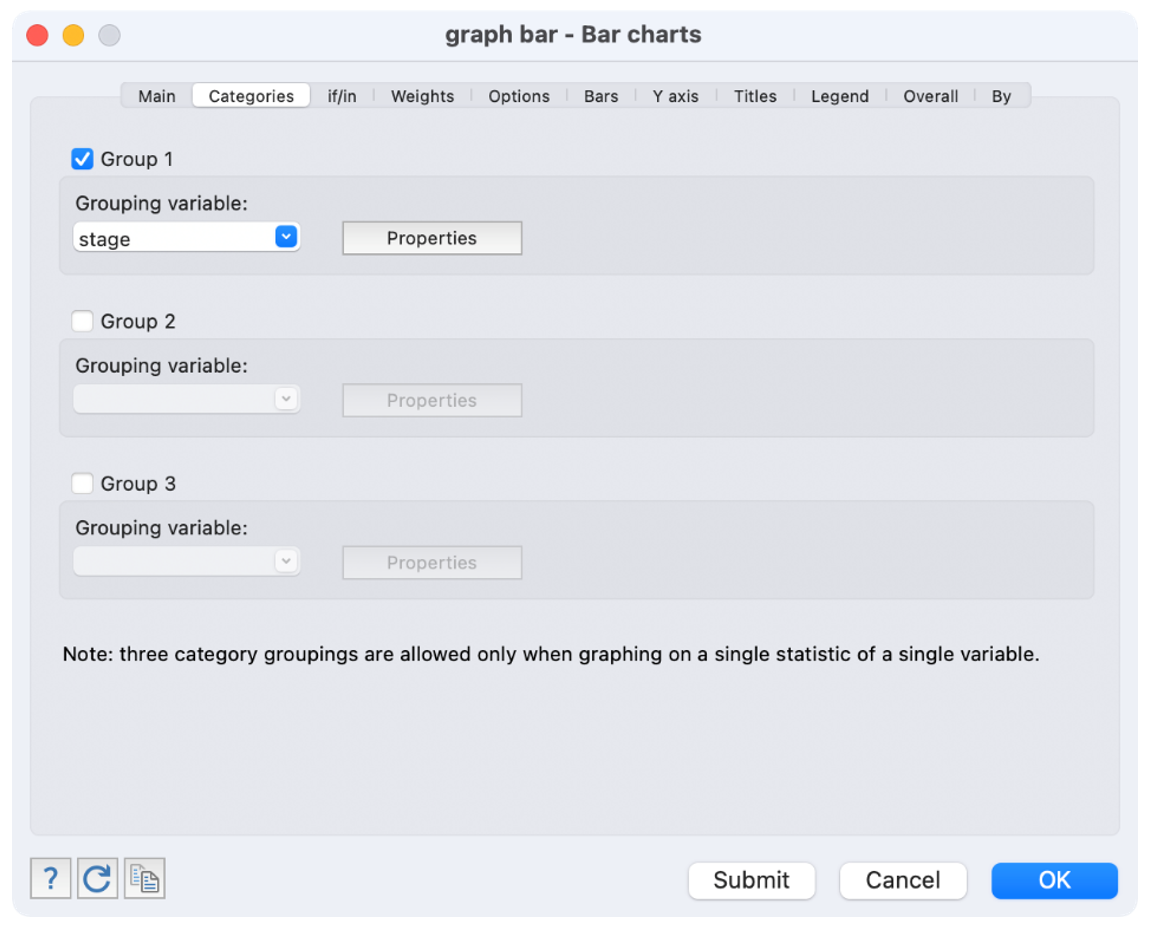
\includegraphics[width=0.75\textwidth,height=\textheight]{img/mod01/stata/bar-02.png}

}

\end{figure}

Click the \textbf{Y axis} tab to include a more meaningful label for the
y axis:

\begin{figure}[H]

{\centering 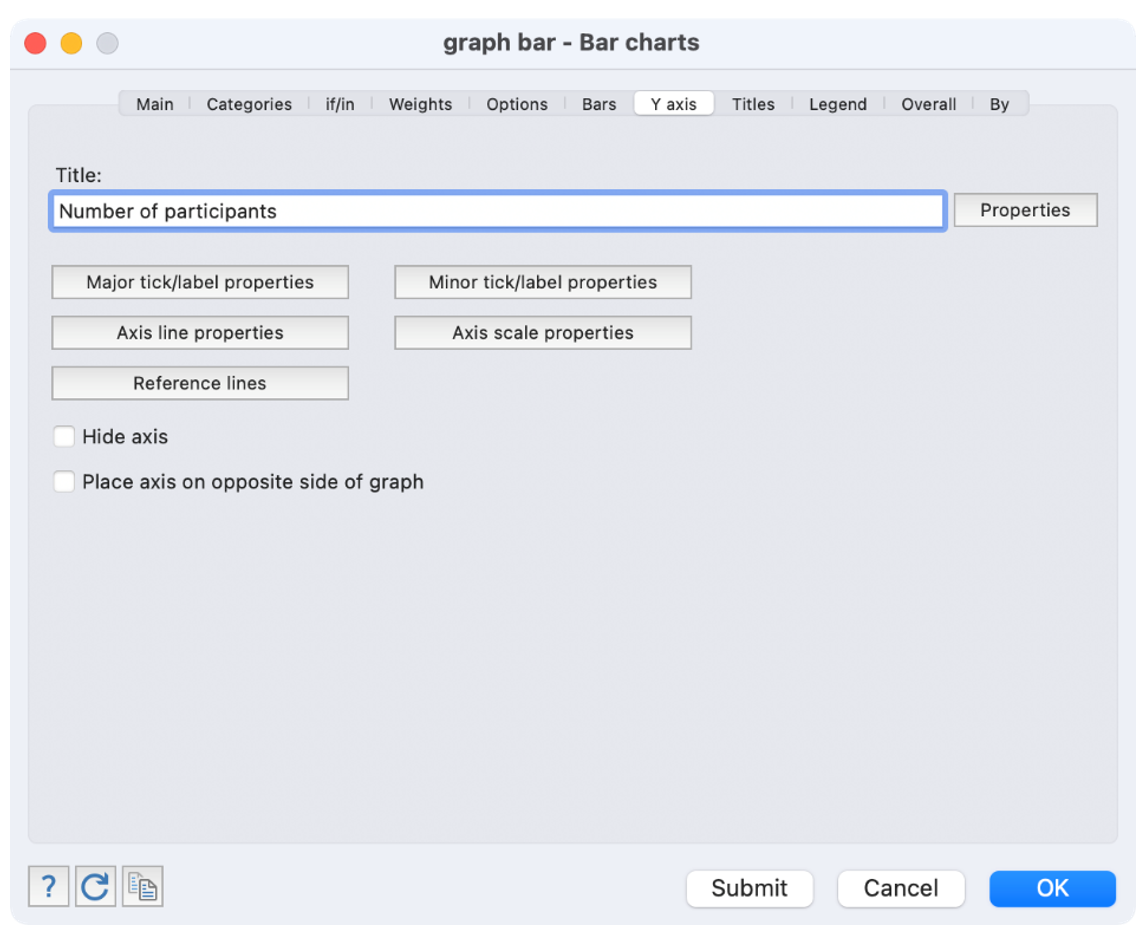
\includegraphics[width=0.75\textwidth,height=\textheight]{img/mod01/stata/bar-03.png}

}

\end{figure}

Click \textbf{Submit} or \textbf{OK}, and the following graph will
appear:

\begin{figure}[H]

{\centering 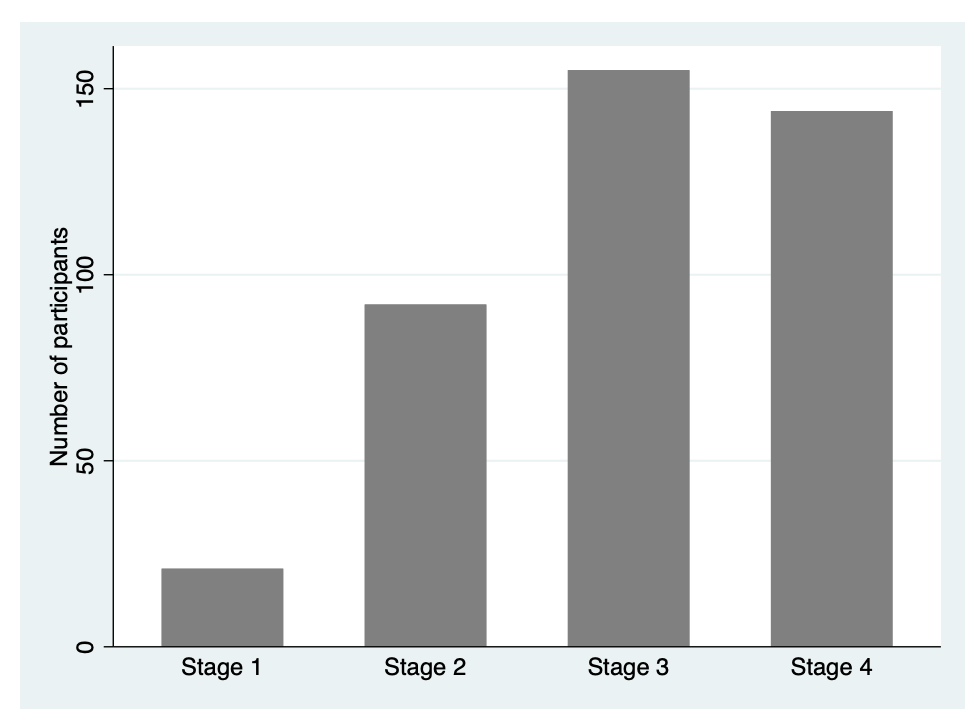
\includegraphics[width=0.75\textwidth,height=\textheight]{img/mod01/stata/bar-04.png}

}

\end{figure}

Note: Value labels have been assigned to stage to create more meaningful
output, and bar colours have been changed to allow for grey-scale
printing.

\hypertarget{submit-vs-ok-button}{%
\subsection{Submit vs OK button}\label{submit-vs-ok-button}}

You may note that most dialog boxes in Stata have two choices: the
\textbf{Submit} button, and the \textbf{OK} button. Both buttons will
submit the command to be run, and both will produce a graph. The
\textbf{Submit} button will submit the command but leave the dialog box
open, while the \textbf{OK} button will submit the command and close the
dialog box. Given the building a graph often involves many incremental
changes, the \textbf{Submit} button is a useful option.

\hypertarget{clustered-bar-graph}{%
\subsection{Clustered bar graph}\label{clustered-bar-graph}}

To create a clustered bar chart as shown in Figure~\ref{fig-bar-2}, go
to: \textbf{Graphics \textgreater{} Bar chart} again. With the previous
settings in place (i.e.~stage as grouping variable and with appropriate
axes labels), now choose \texttt{sex} as the \textbf{Group 1} variable,
and tick \textbf{Group 2} and choose \texttt{stage} as the second
grouping variable.

\begin{figure}[H]

{\centering 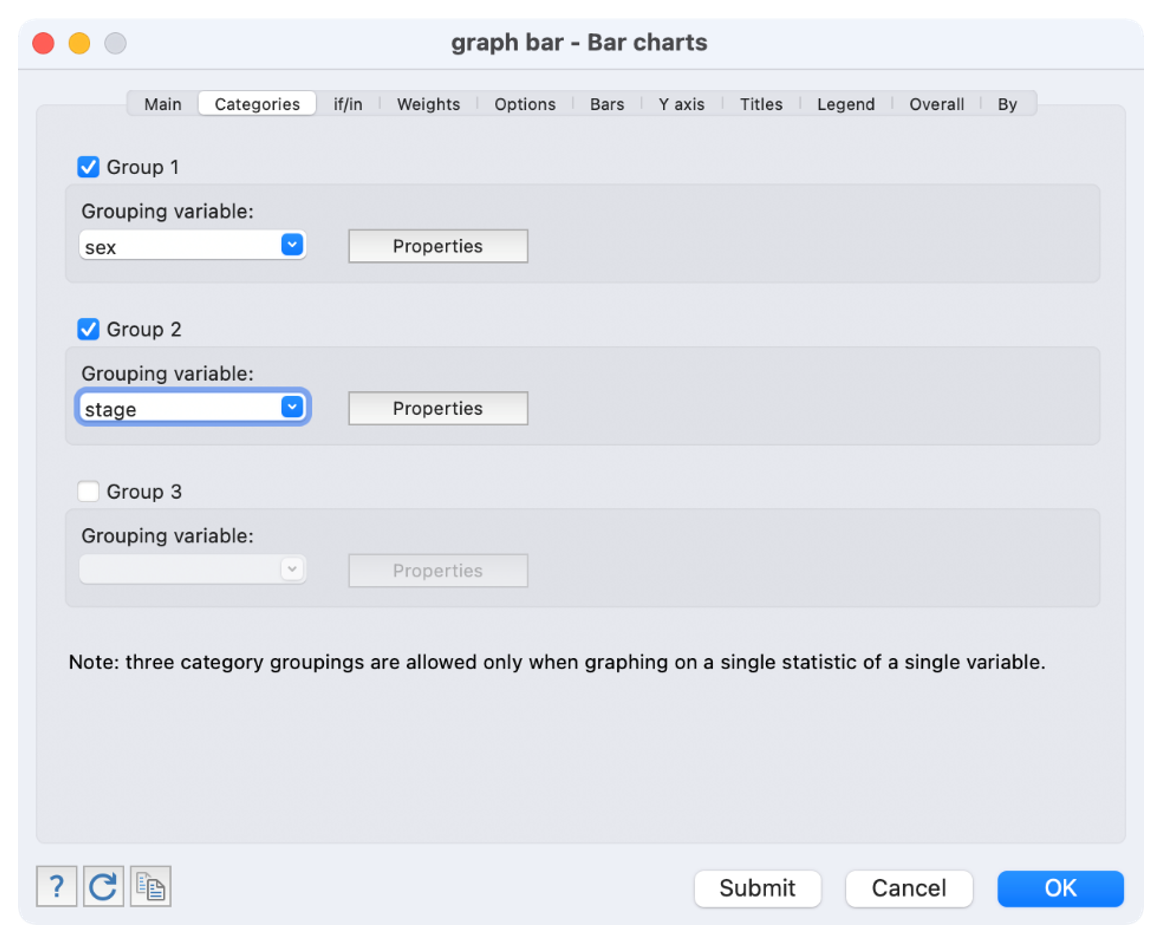
\includegraphics[width=0.75\textwidth,height=\textheight]{img/mod01/stata/bar-05.png}

}

\end{figure}

In the \textbf{Options} tab, tick \textbf{Treat first category grouping
as y variables}. When you are done, click \textbf{OK} or
\textbf{Submit}.

\begin{figure}[H]

{\centering 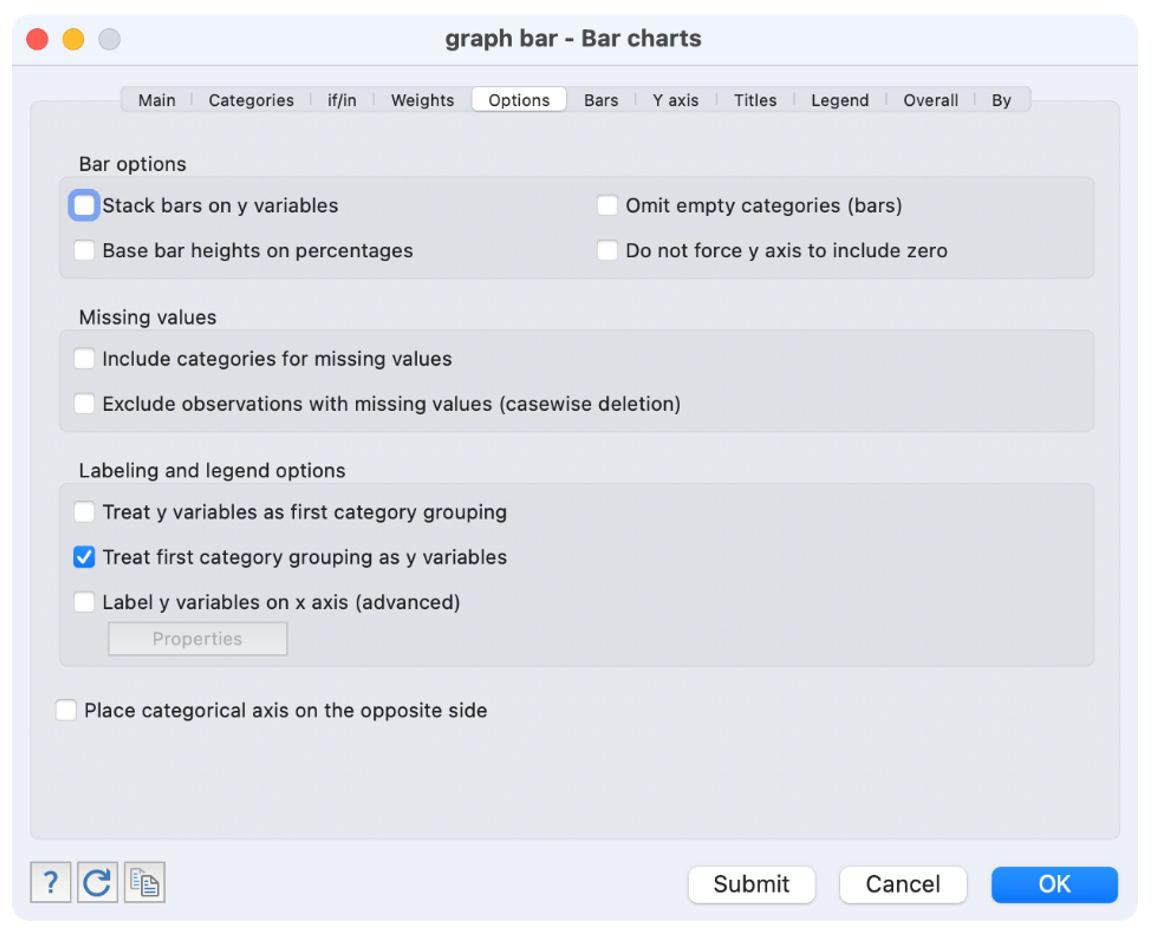
\includegraphics[width=0.75\textwidth,height=\textheight]{img/mod01/stata/bar-06.png}

}

\end{figure}

\begin{figure}[H]

{\centering 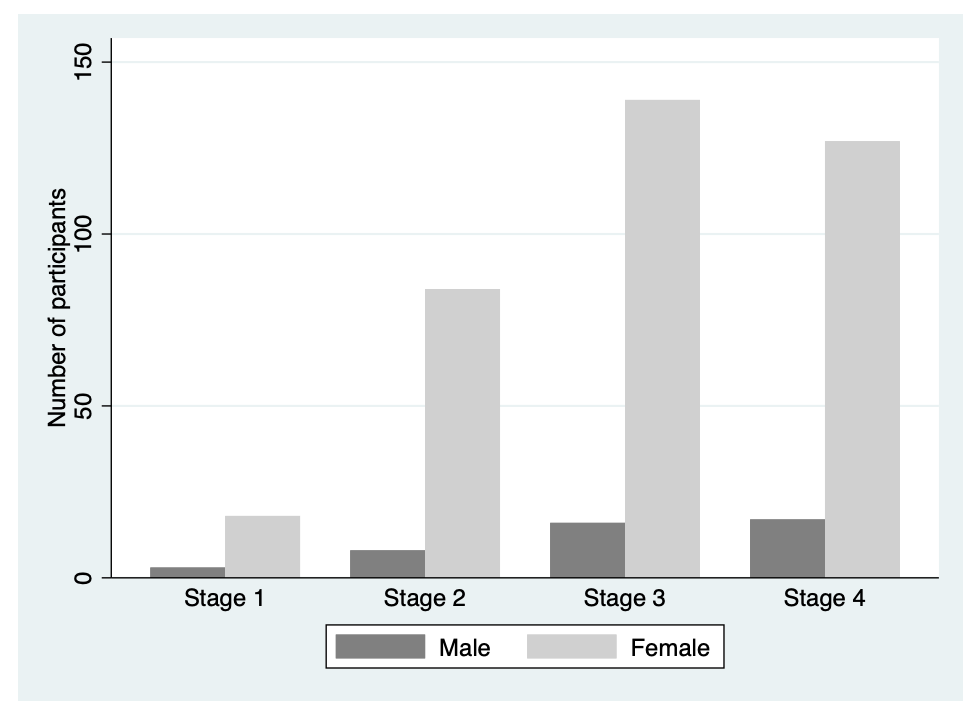
\includegraphics[width=0.75\textwidth,height=\textheight]{img/mod01/stata/bar-07.png}

}

\end{figure}

In a clustered bar chart, the \textbf{Group 2} variable is the main
variable grouping (here, \texttt{stage}), and each of the \textbf{Group
2} categories is split by the \textbf{Group 1} variable (here,
\texttt{sex}).

\hypertarget{stacked-bar-graph}{%
\subsection{Stacked bar graph}\label{stacked-bar-graph}}

To create a stacked bar chart shown in Figure~\ref{fig-bar-3}, bring up
the \textbf{Bar chart} dialog box, go to the \textbf{Options} tab and
tick \textbf{Stack bars on y variables}.

\begin{figure}[H]

{\centering 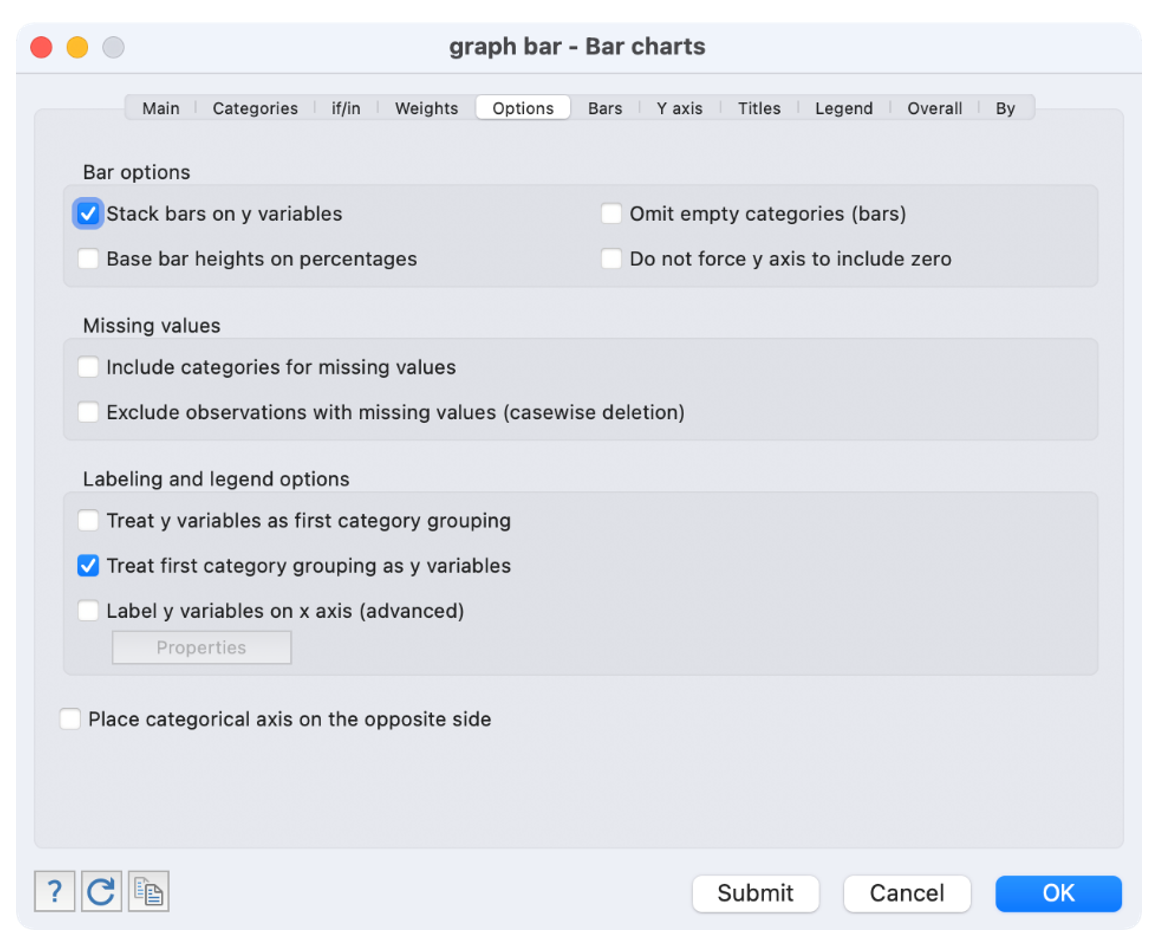
\includegraphics[width=0.75\textwidth,height=\textheight]{img/mod01/stata/bar-08.png}

}

\end{figure}

\begin{figure}[H]

{\centering 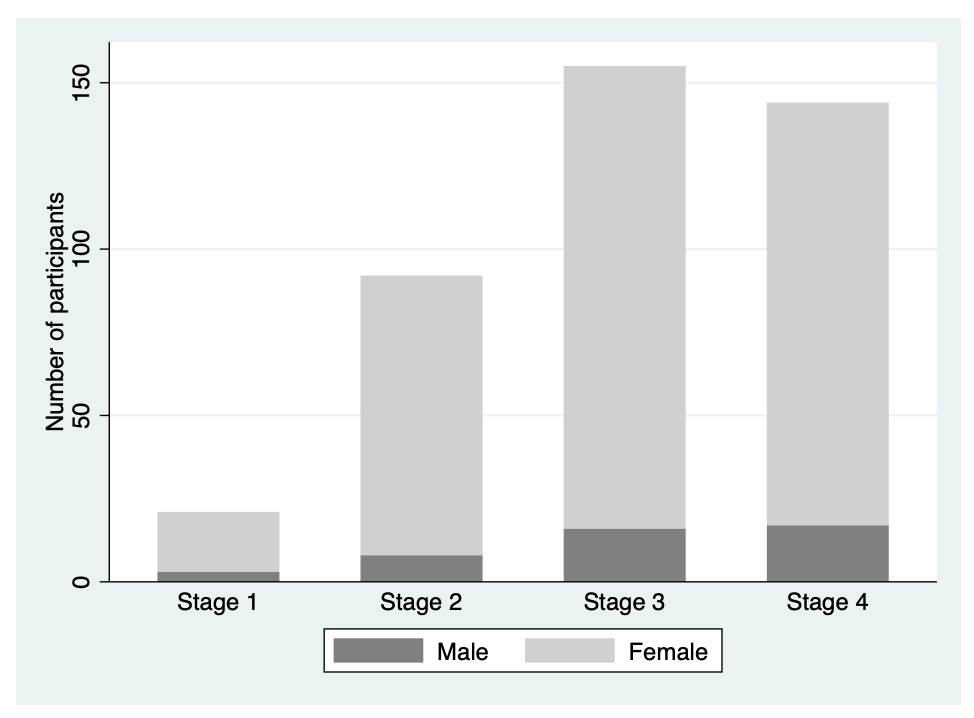
\includegraphics[width=0.75\textwidth,height=\textheight]{img/mod01/stata/bar-10.png}

}

\end{figure}

\hypertarget{stacked-bar-graph-of-relative-frequencies}{%
\subsection{Stacked bar graph of relative
frequencies}\label{stacked-bar-graph-of-relative-frequencies}}

If one wants to compare the sex distribution across the stage
categories, it would be convenient if all the bars have the same height
(100\%). To generate such a bar chart in Stata, tick \textbf{Base bar
heights on percentages} in the \textbf{Options} tab of the \textbf{Bar
charts} dialog box. Change the y-axis title in the \textbf{Y axis} tab
to \texttt{Percentage\ of\ students\ in\ each\ age\ group}.

\begin{figure}[H]

{\centering 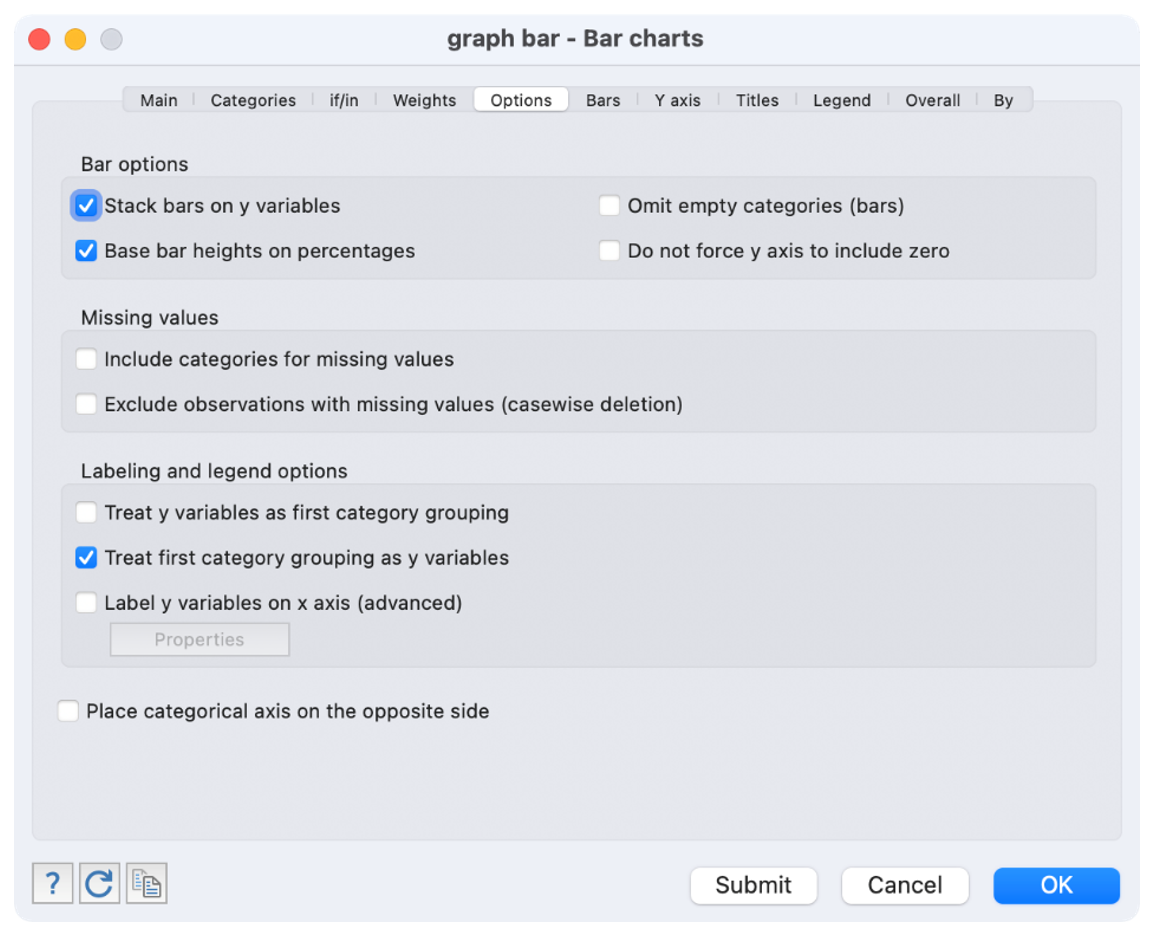
\includegraphics[width=0.75\textwidth,height=\textheight]{img/mod01/stata/bar-11.png}

}

\end{figure}

\begin{figure}[H]

{\centering 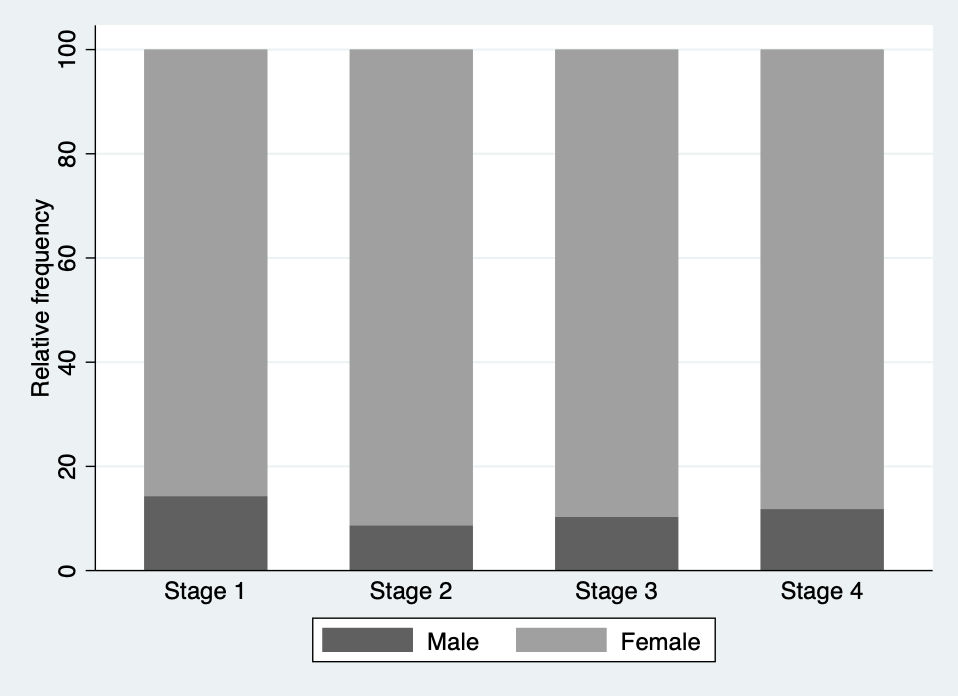
\includegraphics[width=0.75\textwidth,height=\textheight]{img/mod01/stata/bar-12.png}

}

\end{figure}

\hypertarget{editing-graphs-in-stata}{%
\subsection{Editing graphs in Stata}\label{editing-graphs-in-stata}}

There are two main approaches of editing many aspects of a graph (such
as colours, labels, font-size etc). The first approach is to use options
within the dialog boxes. For example, if we wanted to use a
grey-and-white colour scheme for our bar chart, we can define the
colours of the bars in the Bars tab of the bar chart dialog box.

Here, we will define Bar 1 to be \texttt{White}:

\begin{figure}[H]

{\centering 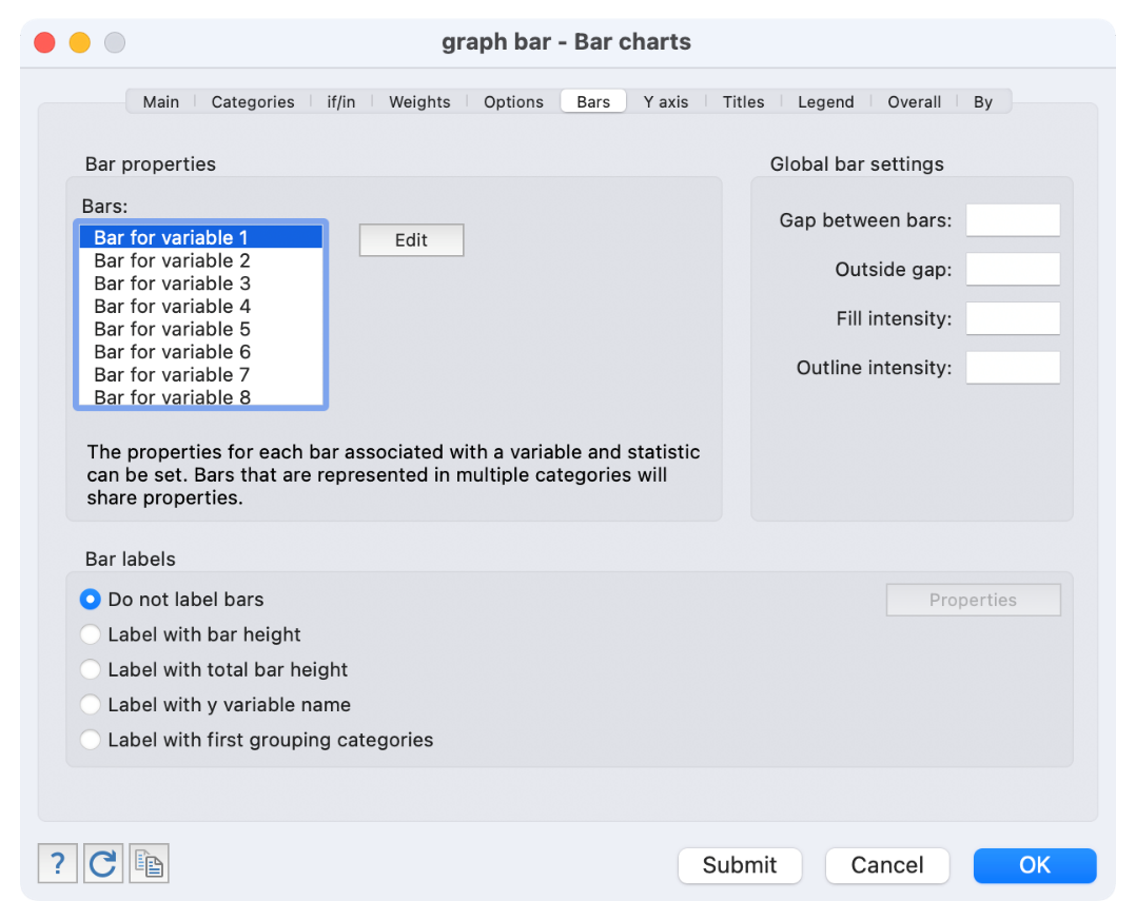
\includegraphics[width=0.75\textwidth,height=\textheight]{img/mod01/stata/edit-01.png}

}

\end{figure}

\begin{figure}[H]

{\centering 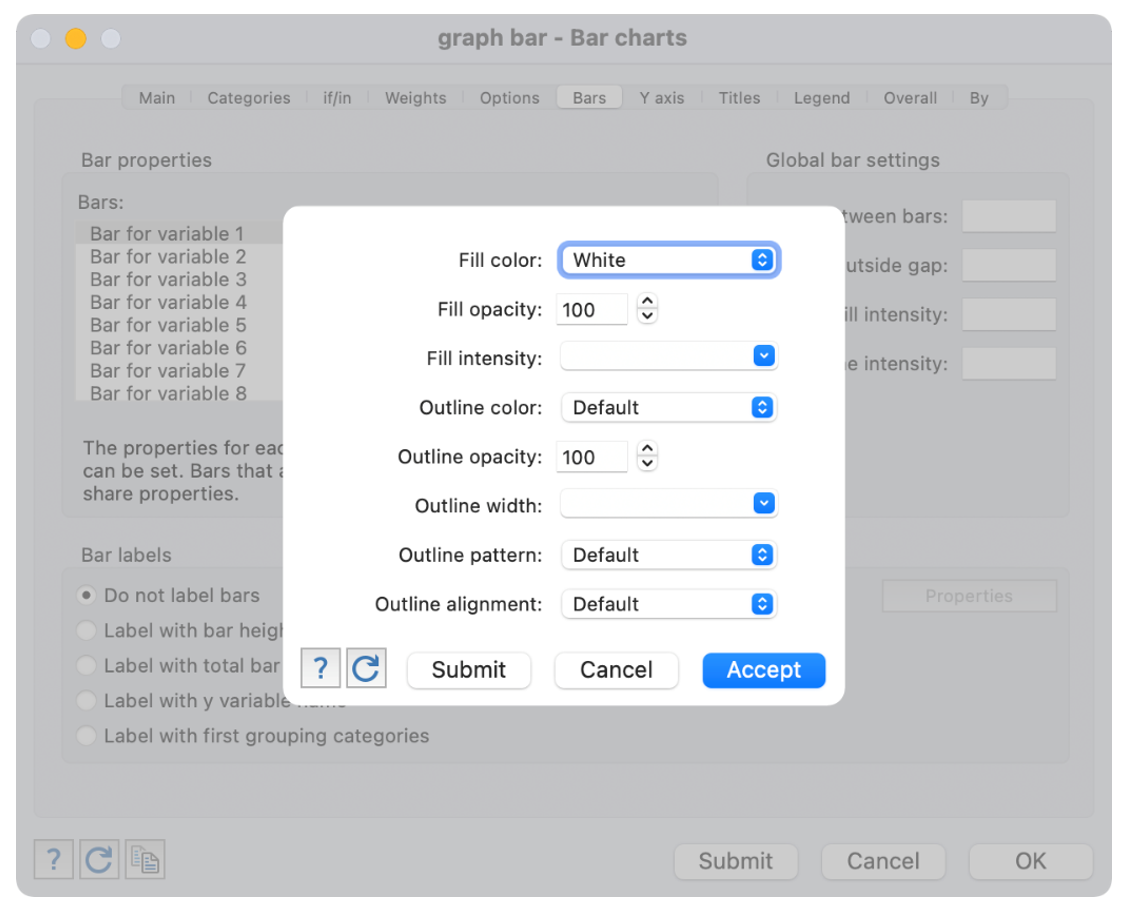
\includegraphics[width=0.75\textwidth,height=\textheight]{img/mod01/stata/edit-02.png}

}

\end{figure}

Bar 2 can be defined to be \texttt{Gray}, resulting in the graph below:

\begin{figure}[H]

{\centering 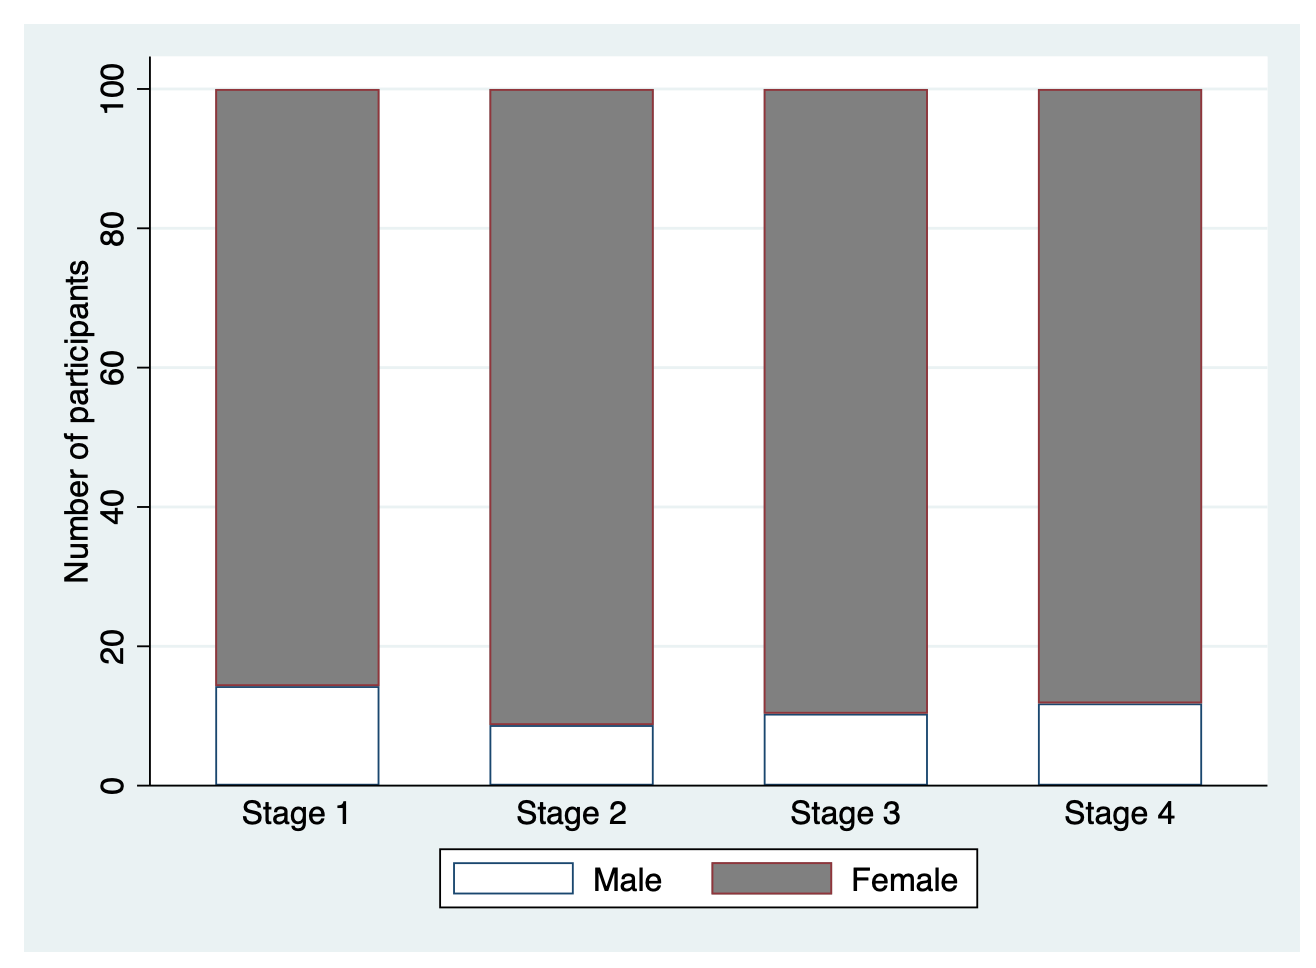
\includegraphics[width=0.75\textwidth,height=\textheight]{img/mod01/stata/edit-03.png}

}

\end{figure}

The second approach to customising graphs is to use the \textbf{Graph
Editor}. Each Stata graph window includes a Graph Editor button:

\begin{figure}[H]

{\centering 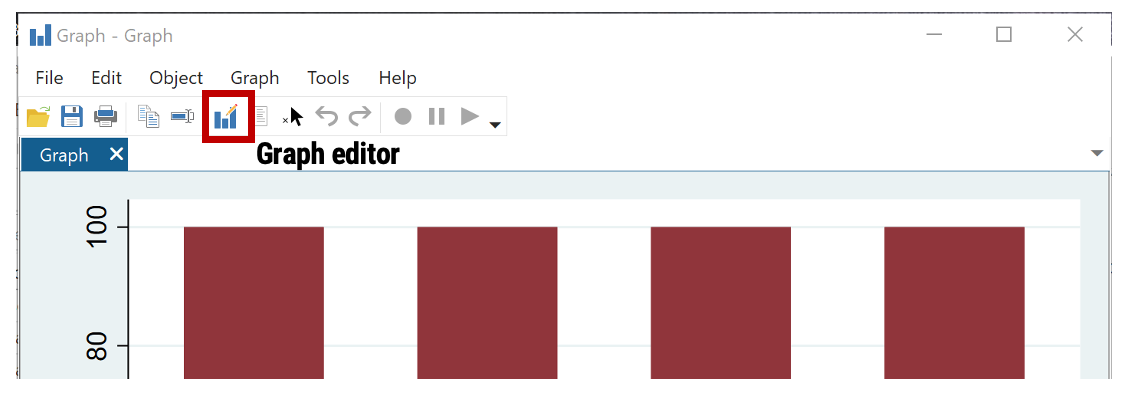
\includegraphics[width=0.75\textwidth,height=\textheight]{img/mod01/stata/edit-04.png}

}

\caption{Graph editor button on Stata for Windows}

\end{figure}

\begin{figure}[H]

{\centering 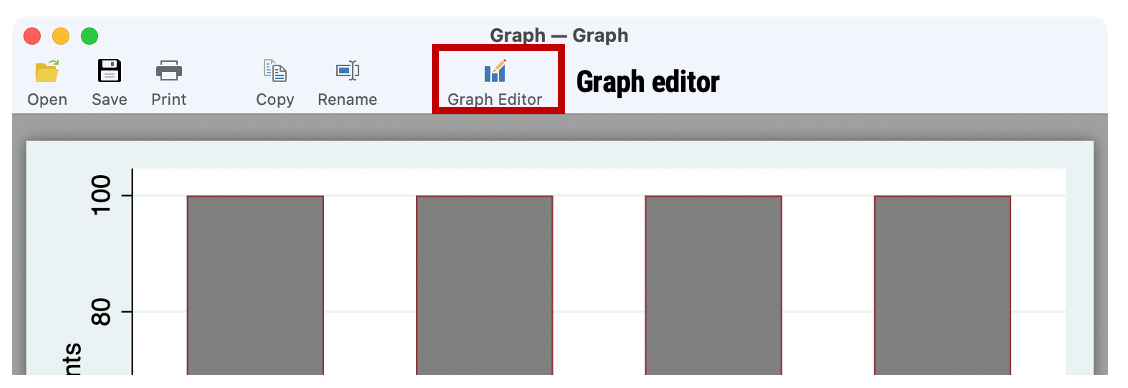
\includegraphics[width=0.75\textwidth,height=\textheight]{img/mod01/stata/edit-05.png}

}

\caption{Graph editor button on Stata for MacOS}

\end{figure}

The \textbf{Graph Editor} window comprises two main sections: the graph
that can be edited on the left, and a list of elements of the graph on
the right. Most aspects of a graph's appearance can be edited in the
Graph Editor, usually by double-clicking an element (e.g.~a bar, or a
bar segment) and changing its properties. There are too many ways to
change a graph's appearance to document here: feel free to explore and
experiment!

\begin{figure}[H]

{\centering 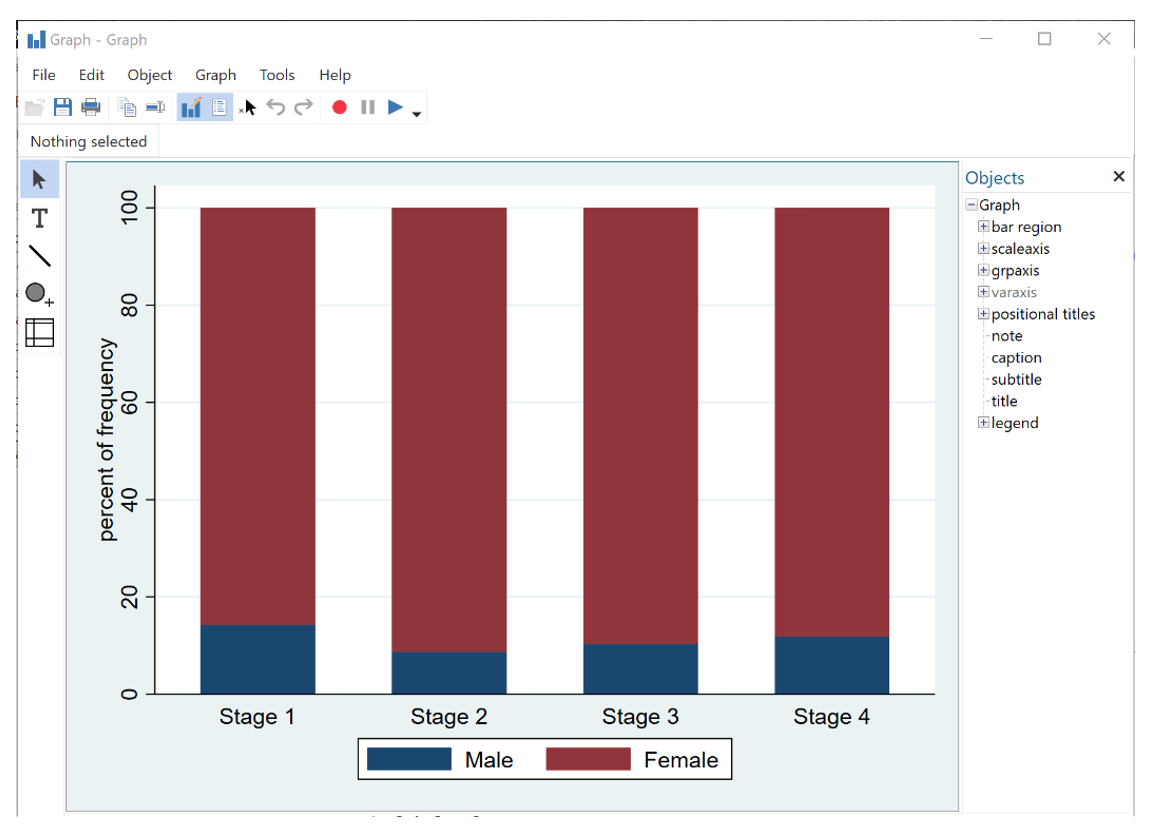
\includegraphics[width=0.75\textwidth,height=\textheight]{img/mod01/stata/edit-06.png}

}

\caption{Graph editor window: Windows}

\end{figure}

\begin{figure}[H]

{\centering \includegraphics[width=0.75\textwidth,height=\textheight]{img/mod01/stata/edit-07.png}

}

\caption{Graph editor window: MacOS}

\end{figure}

When you are done editing in the Graph Editor, click the Graph Editor
icon again to stop the Graph Editor. You will be prompted to save your
graph. You can click the \textbf{Save} button, choose \textbf{Save as}
and choose to save using the \textbf{PNG (*.png)} format. You can then
insert your saved PNG file into your word processing package as usual.

\hypertarget{creating-line-graphs}{%
\subsection{Creating line graphs}\label{creating-line-graphs}}

To demonstrate the graphing of aggregate data with Stata, we use the
data on new cases and deaths from prostate cancer in males in NSW. This
data has been entered into Stata as
\texttt{mod01\_prostate\_cancer.dta}.

If you look at the data in the \textbf{Data Editor} window, you will see
that there are 20 rows - a row for each year of data. Each row contains
the number of new cases (\texttt{NCases}), number of deaths
(\texttt{NDeaths}), the incidence rate (\texttt{RCases}) and death rate
(\texttt{RDeaths}).

To create a line graph as in Figure~\ref{fig-bar-4} select
\textbf{Graphics \textgreater{} Twoway graph (scatter, line, etc.)} and
click the \textbf{Create\ldots{}} button in the \textbf{twoway -- Twoway
graphs} dialog box to bring up a dialog box for defining Plot 1.

\begin{figure}[H]

{\centering \includegraphics[width=0.75\textwidth,height=\textheight]{img/mod01/stata/line-01.png}

}

\end{figure}

Choose \textbf{Line} as the plot type, \texttt{rcases} as the \textbf{Y
variable} and \texttt{year} as the \textbf{X variable} as shown below.

\begin{figure}[H]

{\centering \includegraphics[width=0.75\textwidth,height=\textheight]{img/mod01/stata/line-02.png}

}

\end{figure}

Click \textbf{Accept}, and then click \textbf{Submit} to check how the
graph looks.

\begin{figure}[H]

{\centering \includegraphics[width=0.75\textwidth,height=\textheight]{img/mod01/stata/line-03.png}

}

\end{figure}

This looks ok, but we want to add the death rate to the plot. Click
\textbf{Create\ldots{}} again and add a Plot 2 for mortality rate:

\begin{figure}[H]

{\centering \includegraphics[width=0.75\textwidth,height=\textheight]{img/mod01/stata/line-03-1.png}

}

\end{figure}

Choose \textbf{Line} as the plot type again, \texttt{rdeaths} as the
\textbf{Y} variable and \texttt{year} as the \textbf{X variable}. Click
\textbf{Accept}, and then \textbf{Submit} to check how the graph looks
like now. You should see both variables plotted:

\begin{figure}[H]

{\centering \includegraphics[width=0.75\textwidth,height=\textheight]{img/mod01/stata/line-04.png}

}

\end{figure}

To change the format of either line, click the relevant plot definition
in the main \textbf{twoway} dialog box and click \textbf{Edit}. Click
the \textbf{Line properties} button and choose a \textbf{Pattern}
(e.g.~Short-dash), then click \textbf{Submit} again.

\begin{figure}[H]

{\centering \includegraphics[width=0.75\textwidth,height=\textheight]{img/mod01/stata/line-05.png}

}

\end{figure}

\begin{figure}[H]

{\centering \includegraphics[width=0.75\textwidth,height=\textheight]{img/mod01/stata/line-06.png}

}

\end{figure}

\begin{figure}[H]

{\centering \includegraphics[width=0.75\textwidth,height=\textheight]{img/mod01/stata/line-07.png}

}

\end{figure}

\begin{figure}[H]

{\centering \includegraphics[width=0.75\textwidth,height=\textheight]{img/mod01/stata/line-08.png}

}

\end{figure}

Next, we need an appropriate label for the y-axis. In the main
\textbf{twoway} dialog box, click on the \textbf{Y axis} tab and label
the title appropriately (e.g.~\texttt{Age-standardardised\ rate} and
then click \textbf{OK} or \textbf{Submit}. The graph below should be
produced.

\begin{figure}[H]

{\centering \includegraphics[width=0.75\textwidth,height=\textheight]{img/mod01/stata/line-09.png}

}

\end{figure}

{[}Command:
\texttt{twoway\ (line\ rcases\ year)\ (line\ rdeaths\ year,\ lpattern(shortdash)),\ ytitle(Age-standardised\ rate)}{]}

\newpage{}

\bookmarksetup{startatroot}

\hypertarget{an-introduction-to-r-and-rstudio}{%
\chapter*{An introduction to R and
RStudio}\label{an-introduction-to-r-and-rstudio}}
\addcontentsline{toc}{chapter}{An introduction to R and RStudio}

\markboth{An introduction to R and RStudio}{An introduction to R and
RStudio}

\hypertarget{learning-outcomes-2}{%
\section*{Learning outcomes}\label{learning-outcomes-2}}
\addcontentsline{toc}{section}{Learning outcomes}

\markright{Learning outcomes}

By the end of this Module, you will be able to:

\begin{itemize}
\tightlist
\item
  understand the difference between R and RStudio
\item
  navigate the RStudio interface
\item
  input and import data into R
\item
  use R to summarise data
\item
  perform basic data transformations
\item
  understand the difference between saving R data and saving R output
\item
  copy R output to a standard word processing package
\end{itemize}

\hypertarget{part-1-an-introduction-to-r}{%
\section{Part 1: An introduction to
R}\label{part-1-an-introduction-to-r}}

``R is a language and environment for statistical computing and
graphics.'' \href{https://www.r-project.org/about.html}{Link}. It is an
open-source programming language, used mainly for statistics (including
biostatistics) and data science.

The aim of these notes is to introduce the R language within the RStudio
environment, and to introduce the commands and procedures that are
directly relevant to this course. There is so much more to R than we can
cover in these notes. Relevant information will be provided throughout
the course, and we will provide further references that you can explore
if you are interested.

\hypertarget{r-vs-rstudio}{%
\subsection{R vs RStudio}\label{r-vs-rstudio}}

At its heart, R is a programming language. When you install R on your
computer, you are installing the language and its resources, as well as
a very basic interface for using R. You can write and run R code using
the basic R app, but it's not recommended.

RStudio is an ``Integrated Development Environment'' that runs R while
also providing useful tools to help you write code and analyse data. You
can think of R as an engine which does the work, and RStudio as a car
that uses the engine, but also provides useful tools like GPS navigation
and reversing cameras that help you drive.

Note: even though we recommend that you use RStudio, you still need
install R. \textbf{RStudio will not run without R installed.}

In summary, we recommend you use RStudio to write R code.

\hypertarget{installing-r-and-rstudio}{%
\subsection{Installing R and RStudio}\label{installing-r-and-rstudio}}

\hypertarget{to-install-r-on-your-computer}{%
\subsubsection{To install R on your
computer}\label{to-install-r-on-your-computer}}

\begin{enumerate}
\def\labelenumi{\arabic{enumi}.}
\item
  Download the R installer from:

  \begin{enumerate}
  \def\labelenumii{\alph{enumii}.}
  \tightlist
  \item
    for Windows: \url{https://cran.r-project.org/bin/windows/base/}
  \item
    for MacOS: \url{https://cran.r-project.org/bin/macosx/}
  \end{enumerate}
\item
  Install R by running the installer and following the installation
  instructions. The default settings are fine.

  \begin{itemize}
  \tightlist
  \item
    \textbf{Note for macOS:} if you are running macOS 10.8 or later, you
    will need to install an additional application called XQuartz, which
    is available at \url{https://www.xquartz.org/}. Download the latest
    installer (XQuartz-2.8.5.dmg as of May 2023), and install it in the
    usual way.
  \end{itemize}
\item
  Open the R program. You should see a screen similar to below:
\end{enumerate}

\includegraphics[width=0.8\textwidth,height=\textheight]{img/mod01/R-screenshot.png}

Near the bottom of the R screen, you will find the ``\textgreater{}''
symbol which represents the command line. If you type \texttt{1\ +\ 2}
into the command line and then hit enter you should get:

\texttt{{[}1{]}\ 3}

This is R performing your calculation, with the \texttt{{[}1{]}}
indicating that the solution to \texttt{1\ +\ 2} is a single number (the
number 3).

At this point, close R - we will not interact with R like this in the
future. You can close R by typing \texttt{quit()} at the command prompt,
followed by the return key, or in the usual way of closing an
application in your operating system. There is no need to save anything
here if prompted.

\hypertarget{to-install-rstudio-on-your-computer}{%
\subsubsection{To install RStudio on your
computer}\label{to-install-rstudio-on-your-computer}}

\begin{enumerate}
\def\labelenumi{\arabic{enumi}.}
\tightlist
\item
  Make sure you have already installed R, and verified that it is
  working.
\item
  Download the RStudio desktop installer at:
  \url{https://posit.co/download/rstudio-desktop/}. The website should
  detect your operating system and link to the appropriate installer for
  your computer.
\item
  Install RStudio by running the installer and following the
  installation instructions. The default settings are fine.
\item
  Open RStudio, which will appear similar to the screenshot below:
\end{enumerate}

\includegraphics[width=1\textwidth,height=\textheight]{img/mod01/RStudio-screenshot-01.png}

Locate the command line symbol ``\textgreater{}'' at the bottom of the
left-hand panel. Type \texttt{1\ +\ 2} into the command line and hit
enter, and you will see:

\texttt{{[}1{]}\ 3}

This confirms that RStudio is running correctly, and can use the R
language to correctly calculate the sum between 1 and 2!

RStudio currently comprises three window panes, and we will discuss
these later.

\begin{tcolorbox}[enhanced jigsaw, title={TASK}, opacitybacktitle=0.6, colbacktitle=quarto-callout-note-color!10!white, titlerule=0mm, colframe=quarto-callout-note-color-frame, opacityback=0, left=2mm, breakable, bottomtitle=1mm, coltitle=black, bottomrule=.15mm, arc=.35mm, rightrule=.15mm, toptitle=1mm, colback=white, toprule=.15mm, leftrule=.75mm]

Install R and RStudio and confirm they are both working correctly.

\end{tcolorbox}

\hypertarget{recommended-setup}{%
\subsection{Recommended setup}\label{recommended-setup}}

I will provide a recommended setup for R and RStudio in this section.
You are free to use alternative workflows and setup, but this setup
works well in practice.

\hypertarget{rstudio-preferences}{%
\subsubsection{RStudio preferences}\label{rstudio-preferences}}

By default, RStudio will retain data, scripts and other objects when you
quit your RStudio session. Relying on this can cause headaches, so I
recommend that you set up RStudio so that it does not preserve your
workspace between sessions. Open the RStudio options:

\begin{itemize}
\item
  Mac: \textbf{Edit \textgreater{} Settings}
\item
  Windows: \textbf{Tools \textgreater{} Global Options}
\end{itemize}

and \textbf{deselect ``Restore .RData into workplace at startup''}, and
choose: ``\textbf{Save workspace to .RData on exit:} \textbf{Never''}.

\includegraphics[width=0.75\textwidth,height=\textheight]{img/mod01/RStudio-preferences.png}

\hypertarget{set-up-a-project}{%
\subsubsection{Set up a project}\label{set-up-a-project}}

A project in RStudio is a folder that RStudio recognises as a place to
store R scripts, data files, figures that are common to an analysis
project. Setting up a folder allows much more simple navigation and
specification of data files and output. More detail can be found in
Chapter 8 of the excellent text:
\href{https://r4ds.had.co.nz/workflow-projects.html}{R for Data
Science}. Using projects is not necessary, but I recommend working with
projects from day one.

We will create a project called \textbf{PHCM9795} to store all the data
you will use and scripts that you will write in this course. First,
think about where you want to store your project folder: this could be
somewhere in your \emph{Documents} folder.

Step 1: Choose \textbf{File \textgreater{} New Project\ldots{}} in
RStudio to open the \textbf{Create Project} dialog box:

\includegraphics[width=0.75\textwidth,height=\textheight]{img/mod01/NewProject-1.png}

Step 2: Click the first option to create a project in a \textbf{New
directory}

\includegraphics[width=0.75\textwidth,height=\textheight]{img/mod01/NewProject-2.png}

Step 3: Click the first option: \textbf{New Project}. Give the project a
name, by typing PHCM9795 in the ``Directory name'', and choose where you
want to store the project by clicking the \textbf{Browse} button.

\includegraphics[width=0.75\textwidth,height=\textheight]{img/mod01/NewProject-3.png}

Step 4: Click \textbf{Create} to create your project.

You will now have a new folder in your directory, which contains only
one file: PHCM9795.Rproj, and the two right-hand panes of RStudio will
appear as below:

\includegraphics[width=0.75\textwidth,height=\textheight]{img/mod01/NewProject-4.png}

\begin{tcolorbox}[enhanced jigsaw, title={TASK}, opacitybacktitle=0.6, colbacktitle=quarto-callout-note-color!10!white, titlerule=0mm, colframe=quarto-callout-note-color-frame, opacityback=0, left=2mm, breakable, bottomtitle=1mm, coltitle=black, bottomrule=.15mm, arc=.35mm, rightrule=.15mm, toptitle=1mm, colback=white, toprule=.15mm, leftrule=.75mm]

Create a new project called PHCM9795.

\end{tcolorbox}

The top-right menu bar is showing that you are working within the
PHCM9795 project, and the bottom-right window is showing the contents of
that window: the single PHCM9795.Rproj file. We will add some more files
to this project later.

\hypertarget{sec-simpleR}{%
\subsection{A simple R analysis}\label{sec-simpleR}}

In this very brief section, we will introduce R by calculating the
average of six ages.

To begin, open a new R Script by choosing \textbf{File \textgreater{}
New file \textgreater{} R Script} . A script (or a program) is a
collection of commands that are sequentially processed by R. You can
also type Ctrl+Shift+N in Windows, or Command+Shift+N in MacOS to open a
new script in RStudio, or click the \textbf{New File} button at the top
of the RStudio window.

You should now see four window panes, as below. In the top-left window,
type the following (replacing my name with yours, and including today's
date):

\begin{Shaded}
\begin{Highlighting}[]
\CommentTok{\# Author: Timothy Dobbins}
\CommentTok{\# Date: 5 April 2024}
\CommentTok{\# Purpose: My first R script}

\NormalTok{age }\OtherTok{\textless{}{-}} \FunctionTok{c}\NormalTok{(}\DecValTok{20}\NormalTok{, }\DecValTok{25}\NormalTok{, }\DecValTok{23}\NormalTok{, }\DecValTok{29}\NormalTok{, }\DecValTok{21}\NormalTok{, }\DecValTok{27}\NormalTok{)}
\FunctionTok{summary}\NormalTok{(age)}
\end{Highlighting}
\end{Shaded}

\textbf{Note: R is case-sensitive}, so you should enter the text exactly
as written in these notes.

Your screen should look something like:

\includegraphics[width=1\textwidth,height=\textheight]{img/mod01/RStudio-screenshot-02.png}

To run your script, choose \textbf{Code \textgreater{} Run Region
\textgreater{} Run All}. You will see your code appear in the
bottom-left window, with the following output:

\begin{Shaded}
\begin{Highlighting}[]
\SpecialCharTok{\textgreater{}} \CommentTok{\# Author: Timothy Dobbins}
\ErrorTok{\textgreater{}} \CommentTok{\# Date: 5 April 2022}
\ErrorTok{\textgreater{}} \CommentTok{\# Purpose: My first R script}
\ErrorTok{\textgreater{}} 
\ErrorTok{\textgreater{}}\NormalTok{ age }\OtherTok{\textless{}{-}} \FunctionTok{c}\NormalTok{(}\DecValTok{20}\NormalTok{, }\DecValTok{25}\NormalTok{, }\DecValTok{23}\NormalTok{, }\DecValTok{29}\NormalTok{, }\DecValTok{21}\NormalTok{, }\DecValTok{27}\NormalTok{)}

\SpecialCharTok{\textgreater{}} \FunctionTok{summary}\NormalTok{(age)}
\NormalTok{   Min. 1st Qu.  Median    Mean 3rd Qu.    Max. }
  \FloatTok{20.00}   \FloatTok{21.50}   \FloatTok{24.00}   \FloatTok{24.17}   \FloatTok{26.50}   \FloatTok{29.00} 
\end{Highlighting}
\end{Shaded}

We will explain the key parts of this script later, but for now, you
have entered six ages and calculated the mean age (along with five other
summary statistics).

\begin{tcolorbox}[enhanced jigsaw, title={TASK}, opacitybacktitle=0.6, colbacktitle=quarto-callout-note-color!10!white, titlerule=0mm, colframe=quarto-callout-note-color-frame, opacityback=0, left=2mm, breakable, bottomtitle=1mm, coltitle=black, bottomrule=.15mm, arc=.35mm, rightrule=.15mm, toptitle=1mm, colback=white, toprule=.15mm, leftrule=.75mm]

Type the code above into the top-left window, and run the script.

Save your script within the PHCM9795 project by using \textbf{File
\textgreater{} Save As}, using the name \texttt{my\_first\_analysis.R}.

\end{tcolorbox}

\hypertarget{the-rstudio-environment}{%
\subsection{The RStudio environment}\label{the-rstudio-environment}}

Now that we have seen a simple example of how to use R within RStudio,
let's describe the RStudio environment. Let's assume that you have just
run your first R script, and you have four windows as below:

\includegraphics[width=1\textwidth,height=\textheight]{img/mod01/RStudio-screenshot-03.png}

The top-left window is call the \textbf{Source} window, and is where you
write and edit your R scripts. Scripts can be saved by clicking
\textbf{File \textgreater{} Save As} or by clicking on the symbol of a
floppy disk at the top of the script. The file will have an extension of
.R, for example script.R. Remember to give your script a meaningful
title and remember to periodically save as you go.

In RStudio, the name of the script will be black when it has been saved,
and will change to red if you have any unsaved changes.

The \textbf{Console} window, at the bottom left, contains the command
line which is indicated with the symbol \textgreater. You can type
commands here, but anything executed directly from the console is not
saved and therefore is lost when the session ends (when you exit
RStudio). You should always run your commands from a script file which
you can save and use again later. When you run commands from a script,
the output and any notes/errors are shown in the console. The Terminal
and Jobs tabs will not be used in this course.

The \textbf{Environment} window at the top-right shows a list of objects
that have been created during your session. When you close your RStudio
session these objects will disappear. We will not use the History or
Connections tabs in this course.

The bottom right corner contains some useful tabs, in particular the
\textbf{Help} tab. When you are troubleshooting errors or learning how
to use a function, the Help tab should be the first place you visit.
Here you can search the help documents for all the packages you have
installed. Whenever you create plots in R, these will be shown in the
\textbf{Plots} tab. The \textbf{Packages} tab contains a list of
installed packages and indicates which ones are currently in use (we
will learn about packages later). Packages which are loaded, i.e.~in
use, are indicated with a tick. Some packages are in use by default when
you begin a new session. You can access information about a package by
clicking on its name. The \textbf{Files} tab provides a shortcut to
access your files. The Viewer tab will not be used in this course.

\hypertarget{some-r-basics}{%
\subsection{Some R basics}\label{some-r-basics}}

While we use R as a statistics package, R is a programming language. In
order to use R effectively, we need to define some basics.

\hypertarget{scripts}{%
\subsubsection{Scripts}\label{scripts}}

While R can be run completely from the command line, issuing commands
one-by-one, it is most commonly run using \textbf{scripts}. A script is
simply a list of commands that are processed in order. The simple
analysis we conducted earlier is a very simple script. Some things to
know about R scripts:

\begin{itemize}
\item
  anything appearing after a \# is a comment, and is ignored by R. The
  first three lines of our script are there for ourselves (either as
  writers of code, or readers of code). I include comments at the
  beginning of each of my scripts to describe:

  \begin{itemize}
  \item
    who wrote the script (useful if someone else uses your script and
    wants to ask questions about it);
  \item
    when the script was written;
  \item
    what the script does. This last point may seem odd, but it's useful
    to describe what this script does, and why it might differ to other
    scripts being used in the analysis. This is particularly useful if
    your scripts become long and complex.
  \end{itemize}
\item
  \textbf{R is case-sensitive}. So \texttt{age}, \texttt{AGE} and
  \texttt{Age} could refer to three separate variables (please don't do
  this!)
\item
  use blank lines and comments to separate sections of your script
\end{itemize}

\hypertarget{objects}{%
\subsubsection{Objects}\label{objects}}

If you do some reading about R, you may learn that R is an
``object-oriented programming language''. When we enter or import data
into R, we are asking R to create \textbf{objects} from our data. These
objects can be manipulated and transformed by \textbf{functions}, to
obtain useful insights from our data.

Objects in R are created using the \textbf{assignment operator}. The
most common form of the assignment operator looks like an arrow:
\texttt{\textless{}-} and is typed as the \texttt{\textless{}} and
\texttt{-} symbols. The simplest way of reading \texttt{\textless{}-} is
as the words ``is defined as''. Note that it possible to use
\texttt{-\textgreater{}} and even \texttt{=} as assignment operators,
but their use is less frequent.

Let's see an example:

\begin{Shaded}
\begin{Highlighting}[]
\NormalTok{x }\OtherTok{\textless{}{-}} \DecValTok{42}
\end{Highlighting}
\end{Shaded}

This command creates a new object called \texttt{x}, which is defined as
the number 42 (or in words, ``\texttt{x} is defined as 42''). Running
this command gives no output in the console, but the new object appears
in the top-right \textbf{Environment} panel. We can view the object in
the console by typing its name:

\begin{Shaded}
\begin{Highlighting}[]
\CommentTok{\# Print the object x}
\NormalTok{x}
\end{Highlighting}
\end{Shaded}

\begin{verbatim}
[1] 42
\end{verbatim}

Now we see the contents of \texttt{x} in the console.

This example is rather trivial, and we rarely assign objects of just one
value. In fact, we created an object earlier, called \texttt{age}, which
comprised six values.

\hypertarget{sec-data-structures}{%
\subsubsection{Data structures}\label{sec-data-structures}}

There are two main structures we will use to work with data in this
course: \textbf{vectors} and \textbf{data frames}. A \textbf{vector} is
a combination of data values, all of the same type. For example, our six
ages that we entered earlier is a vector. You could think of a vector as
a column of data (even though R prints vectors as rows!) And
technically, even an object with only one value is a vector, a vector of
size 1.

The easiest way of creating a vector in R is by using the \texttt{c()}
function, where c stands for `combine'. In our previous Simple Analysis
in R (Section~\ref{sec-simpleR}), we wrote the command:

\begin{Shaded}
\begin{Highlighting}[]
\NormalTok{age }\OtherTok{\textless{}{-}} \FunctionTok{c}\NormalTok{(}\DecValTok{20}\NormalTok{, }\DecValTok{25}\NormalTok{, }\DecValTok{23}\NormalTok{, }\DecValTok{29}\NormalTok{, }\DecValTok{21}\NormalTok{, }\DecValTok{27}\NormalTok{)}
\end{Highlighting}
\end{Shaded}

This command created a new object called \texttt{age}, and
\emph{combined} the six values of age into one vector.

Just as having a vector of size 1 is unusual, having just one column of
data to analyse is also pretty unusual. The other structure we will
describe here is a \textbf{data frame} which is essentially a collection
of vectors, each of the same size. You could think of a data frame as
being like a spreadsheet, with columns representing variables, and rows
representing observations.

There are other structures in R, such as matrices and lists, which we
won't discuss in this course. And you may come across the term
\textbf{tibble}, which is a type of data frame.

\hypertarget{functions}{%
\subsubsection{Functions}\label{functions}}

If objects are the nouns of R, functions are the verbs. Essentially,
functions transform objects. Functions can transform your data into
summary statistics, graphical summaries or analysis results. For
example, we used the \texttt{summary()} function to display summary
statistics for our six ages.

R functions are specified by their arguments (or inputs). The arguments
that can be supplied for each function can be inspected by examining the
help notes for that function. To obtain help for a function, we can
submit \texttt{help(summary)} (or equivalently \texttt{?summary}) in the
console, or we can use the \textbf{Help} tab in the bottom-right window
of RStudio. For example, the first part of the help notes for
\texttt{summary} appear as:

\includegraphics[width=0.8\textwidth,height=\textheight]{img/mod01/help-1.png}

The help notes in R can be quite cryptic, but the \textbf{Usage} section
details what inputs should be specified for the function to run. Here,
\texttt{summary} requires an object to be specified. In our case, we
specified \texttt{age}, which is our object defined as the vector of six
ages.

Most help pages also include some examples of how you might use the
function. These can be found at the very bottom of the help page.

\includegraphics[width=0.8\textwidth,height=\textheight]{img/mod01/help-2.png}

The \texttt{summary()} function is quite simple, in that it only
requires one input, the object to be summarised. More complex functions
might require a number of inputs. For example, the help notes for the
\texttt{descriptives()} function in the \texttt{jmv} package show a
large number of inputs can be specified:

\includegraphics[width=0.8\textwidth,height=\textheight]{img/mod01/help-3.png}

There are two things to note here. First, notice that the first two
inputs are listed with no = symbol, but all other inputs are listed with
= symbols (with values provided after the = symbol). This means that
everything apart from \texttt{data} and \texttt{vars} have
\textbf{default} values. We are free to not specify values for these
inputs if we are happy with the defaults provided. For example, by
default the variance is not calculated (as \texttt{variance\ =\ FALSE}).
To obtain the variance as well as the standard deviation, we can change
this default to \texttt{variance\ =\ TRUE}:

\begin{Shaded}
\begin{Highlighting}[]
\CommentTok{\# Only the standard deviation is provided as the measure of variability}
\FunctionTok{descriptives}\NormalTok{(}\AttributeTok{data=}\NormalTok{pbc, }\AttributeTok{vars=}\NormalTok{age)}

\CommentTok{\# Additionally request the variance to be calculated}
\FunctionTok{descriptives}\NormalTok{(}\AttributeTok{data=}\NormalTok{pbc, }\AttributeTok{vars=}\NormalTok{age, }\AttributeTok{variance=}\ConstantTok{TRUE}\NormalTok{)}
\end{Highlighting}
\end{Shaded}

Second, for functions with multiple inputs, we can specify the input
name and its value, or we can ignore the input name and specify just the
input values \textbf{in the order listed in the Usage section}. So the
following are equivalent:

\begin{Shaded}
\begin{Highlighting}[]
\CommentTok{\# We can specify that the dataset to be summarised is pbc,}
\CommentTok{\#   and the variable to summarise is age:}
\FunctionTok{descriptives}\NormalTok{(}\AttributeTok{data=}\NormalTok{pbc, }\AttributeTok{vars=}\NormalTok{age)}

\CommentTok{\# We can omit the input name, as long as we keep the inputs in the correct order {-} }
\CommentTok{\#   that is, dataset first, variable second:}
\FunctionTok{descriptives}\NormalTok{(pbc, age)}

\CommentTok{\# We can change the order of the inputs, as long as we specify the input name:}
\FunctionTok{descriptives}\NormalTok{(}\AttributeTok{vars=}\NormalTok{age, }\AttributeTok{data=}\NormalTok{pbc)}
\end{Highlighting}
\end{Shaded}

In this course, we will usually provide all the input names, even when
they are not required. As you become more familiar with R, you will
start to use the shortcut method.

\hypertarget{the-curse-of-inconsistency}{%
\subsubsection{The curse of
inconsistency}\label{the-curse-of-inconsistency}}

As R is an open-source project, many people have contributed to its
development. This has led to a frustrating part of R: some functions
require a single object to be specified, but some require you to specify
a data frame and select variables for analysis. Let's see an example.

The help for \texttt{summary()} specifies the usage as:
\texttt{summary(object,\ ...)}. This means we need to specify a single
object to be summarised. An object could be a single column of data
(i.e.~a vector), or it could be a data frame. If we have a data frame
called \texttt{pbc} which contains many variables, the command
\texttt{summary(pbc)} would summarise every variable in the data frame.

What if we only wanted to summarise the age of the participants in the
data frame? To select a single variable from a data frame, we can use
the following syntax: \texttt{dataframe\$variable}. So to summarise just
age from this data frame, we would use: \texttt{summary(pbc\$age)}.

Compare this with the \texttt{descriptives()} function in the
\texttt{jmv} package. We saw earlier that the two required inputs for
\texttt{descriptives()} are \texttt{data} (the data frame to be
analysed) and \texttt{vars} (the variables to be analysed). So to
summarise \texttt{age} from the \texttt{pbc} data frame, we would
specify \texttt{descriptives(data=pbc,\ vars=age)}.

This inconsistency will seem maddening at first, and will continue to be
maddening! Reading the \textbf{usage} section of the help pages is a
useful way to determine whether you should specify an object (like
\texttt{pbc\$age}) or a data frame and a list of variables.

\hypertarget{packages}{%
\subsection{Packages}\label{packages}}

A \textbf{package} is a collection of functions, documentation (and
sometimes datasets) that extend the capabilities of R. Packages have
been written by R users to be freely distributed and used by others. R
packages can be obtained from many sources, but the most common source
is CRAN: the Comprehensive R Archive Network.

A useful way of thinking about R is that R is like a smartphone, with
packages being like apps which are downloaded from CRAN (similar to an
app-store). When you first install R, it comes with a basic set of
packages (apps) installed. You can do a lot of things with these basic
packages, but sometimes you might want to do things differently, or you
may want to perform some analyses that can't be done using the default
packages. In these cases, you can install a package.

Like installing an app on a smartphone, you only need to \emph{install}
a package once. But each time you want to use the package, you need to
\emph{load} the package into R.

\hypertarget{how-to-install-a-package}{%
\subsubsection{How to install a
package}\label{how-to-install-a-package}}

There are a couple of ways to install a package. You can use the
\texttt{install.packages()} function if you know the exact name of the
package. Let's use an example of installing the \texttt{skimr} package,
which gives a very nice, high-level overview of any data frame. We can
install \texttt{skimr} by typing the following into the console:

\begin{Shaded}
\begin{Highlighting}[]
\FunctionTok{install.packages}\NormalTok{(}\StringTok{"skimr"}\NormalTok{)}
\end{Highlighting}
\end{Shaded}

Note the use of the quotation marks.

Alternatively, RStudio offers a graphical way of installing packages
that can be accessed via \textbf{Tools \textgreater{} Install Packages},
or via the \textbf{Install} button at the top of the \textbf{Packages}
tab in the bottom-right window. You can begin typing the name of the
package in the dialog box that appears, and RStudio will use predictive
text to offer possible packages:

\includegraphics[width=0.6\textwidth,height=\textheight]{img/mod01/install-packages.png}

While writing code is usually the recommended way to use R, installing
packages is an exception. Using \textbf{Tools \textgreater{} Install
Packages} is perfectly fine, because you only need to install a package
once.

\hypertarget{how-to-load-a-package}{%
\subsubsection{How to load a package}\label{how-to-load-a-package}}

When you begin a new session in RStudio, i.e.~when you open RStudio,
only certain core packages are automatically loaded. You can use the
\texttt{library()} function to load a package that you has previously
been installed. For example, now that we have installed \texttt{skimr},
we need to load it before we can use it:

\begin{Shaded}
\begin{Highlighting}[]
\FunctionTok{library}\NormalTok{(skimr)}
\end{Highlighting}
\end{Shaded}

Note that quotation marks are not required for the \texttt{library()}
function (although they can be included if you really like quotation
marks!).

\begin{tcolorbox}[enhanced jigsaw, title={TASK}, opacitybacktitle=0.6, colbacktitle=quarto-callout-note-color!10!white, titlerule=0mm, colframe=quarto-callout-note-color-frame, opacityback=0, left=2mm, breakable, bottomtitle=1mm, coltitle=black, bottomrule=.15mm, arc=.35mm, rightrule=.15mm, toptitle=1mm, colback=white, toprule=.15mm, leftrule=.75mm]

Install the package \texttt{jmv} using \textbf{Tools \textgreater{}
Install packages}, or by typing into the console:

\texttt{install.packages("jmv")}

\end{tcolorbox}

\hypertarget{installing-vs-loading-packages}{%
\subsubsection{Installing vs loading
packages}\label{installing-vs-loading-packages}}

Package installation:

\begin{itemize}
\tightlist
\item
  use the \texttt{install.packages()} function (note the `s') or
  \textbf{Tools \textgreater{} Install packages}
\item
  the package name must be surrounded by quotation marks
\item
  only needs to be done once
\end{itemize}

Package loading

\begin{itemize}
\tightlist
\item
  use the \texttt{library()} function
\item
  the package name does not need to be surrounded by quotation marks
\item
  must be done for each R session
\end{itemize}

\hypertarget{what-is-this-thing-called-the-tidyverse}{%
\subsection{What is this thing called the
tidyverse?}\label{what-is-this-thing-called-the-tidyverse}}

If you have done much reading about R, you may have come across the
tidyverse:

\begin{quote}
``The tidyverse is an opinionated collection of R packages designed for
data science. All packages share an underlying design philosophy,
grammar, and data structures.'' \url{https://www.tidyverse.org/}
\end{quote}

Packages in the tidyverse have been designed with a goal to make using R
more consistent by defining a ``grammar'' to manipulate data, examine
data and draw conclusions from data. While the tidyverse is a common and
powerful set of packages, we will not be teaching the tidyverse in this
course for two main reasons:

\begin{enumerate}
\def\labelenumi{\arabic{enumi}.}
\tightlist
\item
  The data we provide have been saved in a relatively tidy way, and do
  not need much manipulation for analyses to be conducted. The cognitive
  load in learning the tidyverse in this course is greater than the
  benefit that could be gained.
\item
  There are many resources (online, in print etc) that are based on
  \texttt{base\ R}, and do not use the tidyverse. It would be difficult
  to understand these resources if we taught only tidyverse techniques.
  In particular, the \texttt{dataframe\$variable} syntax is an important
  concept that should be understood before moving into the tidyverse.
\end{enumerate}

In saying all of this, I think the tidyverse is an excellent set of
packages, which I frequently use. At the completion of this course, you
will be well equipped to teach yourself tidyverse using many excellent
resources such as:
\href{https://jhudatascience.org/tidyversecourse/}{Tidyverse Skills for
Data Science} and \href{https://r4ds.had.co.nz/}{R for Data Science}.

\hypertarget{part-2-obtaining-basic-descriptive-statistics-1}{%
\section{Part 2: Obtaining basic descriptive
statistics}\label{part-2-obtaining-basic-descriptive-statistics-1}}

In this exercise, we will analyse data to complete a descriptive table
from a research study. The data come from a study in primary biliary
cirrhosis, a condition of the liver, from Modeling Survival Data:
Extending the Cox Model Therneau and Grambsch (2010). By the end of this
exercise, we will have completed the following table.

 
  \providecommand{\huxb}[2]{\arrayrulecolor[RGB]{#1}\global\arrayrulewidth=#2pt}
  \providecommand{\huxvb}[2]{\color[RGB]{#1}\vrule width #2pt}
  \providecommand{\huxtpad}[1]{\rule{0pt}{#1}}
  \providecommand{\huxbpad}[1]{\rule[-#1]{0pt}{#1}}

\begin{table}[ht]
\begin{centerbox}
\begin{threeparttable}
\captionsetup{justification=centering,singlelinecheck=off}
\caption{Summary of 418 participants from the PBC study (Therneau and Grambsch, 2000)}
 \setlength{\tabcolsep}{0pt}
\begin{tabularx}{0.95\textwidth}{p{0.316666666666667\textwidth} p{0.316666666666667\textwidth} p{0.316666666666667\textwidth}}


\hhline{>{\huxb{0, 0, 0}{0.4}}->{\huxb{0, 0, 0}{0.4}}->{\huxb{0, 0, 0}{0.4}}-}
\arrayrulecolor{black}

\multicolumn{1}{!{\huxvb{0, 0, 0}{0}}p{0.316666666666667\textwidth}!{\huxvb{0, 0, 0}{0}}}{\hspace{0pt}\parbox[b]{0.316666666666667\textwidth-0pt-6pt}{\huxtpad{6pt + 1em}\raggedright \textbf{Characteristic}\huxbpad{6pt}}} &
\multicolumn{1}{p{0.316666666666667\textwidth}!{\huxvb{0, 0, 0}{0}}}{\hspace{6pt}\parbox[b]{0.316666666666667\textwidth-6pt-6pt}{\huxtpad{6pt + 1em}\raggedright \textbf{ }\huxbpad{6pt}}} &
\multicolumn{1}{p{0.316666666666667\textwidth}!{\huxvb{0, 0, 0}{0}}}{\hspace{6pt}\parbox[b]{0.316666666666667\textwidth-6pt-0pt}{\huxtpad{6pt + 1em}\raggedright \textbf{Summary}\huxbpad{6pt}}} \tabularnewline[-0.5pt]


\hhline{>{\huxb{0, 0, 0}{0.4}}->{\huxb{0, 0, 0}{0.4}}->{\huxb{0, 0, 0}{0.4}}-}
\arrayrulecolor{black}

\multicolumn{1}{!{\huxvb{0, 0, 0}{0}}p{0.316666666666667\textwidth}!{\huxvb{0, 0, 0}{0}}}{\hspace{0pt}\parbox[b]{0.316666666666667\textwidth-0pt-6pt}{\huxtpad{6pt + 1em}\raggedright Age (years)\huxbpad{6pt}}} &
\multicolumn{1}{p{0.316666666666667\textwidth}!{\huxvb{0, 0, 0}{0}}}{\hspace{6pt}\parbox[b]{0.316666666666667\textwidth-6pt-6pt}{\huxtpad{6pt + 1em}\raggedright \huxbpad{6pt}}} &
\multicolumn{1}{p{0.316666666666667\textwidth}!{\huxvb{0, 0, 0}{0}}}{\hspace{6pt}\parbox[b]{0.316666666666667\textwidth-6pt-0pt}{\huxtpad{6pt + 1em}\raggedright Mean (SD) or Median [IQR]\huxbpad{6pt}}} \tabularnewline[-0.5pt]


\hhline{}
\arrayrulecolor{black}

\multicolumn{1}{!{\huxvb{0, 0, 0}{0}}p{0.316666666666667\textwidth}!{\huxvb{0, 0, 0}{0}}}{} &
\multicolumn{1}{p{0.316666666666667\textwidth}!{\huxvb{0, 0, 0}{0}}}{\hspace{6pt}\parbox[b]{0.316666666666667\textwidth-6pt-6pt}{\huxtpad{6pt + 1em}\raggedright Male\huxbpad{6pt}}} &
\multicolumn{1}{p{0.316666666666667\textwidth}!{\huxvb{0, 0, 0}{0}}}{\hspace{6pt}\parbox[b]{0.316666666666667\textwidth-6pt-0pt}{\huxtpad{6pt + 1em}\raggedright n (\%)\huxbpad{6pt}}} \tabularnewline[-0.5pt]


\hhline{}
\arrayrulecolor{black}

\multicolumn{1}{!{\huxvb{0, 0, 0}{0}}p{0.316666666666667\textwidth}!{\huxvb{0, 0, 0}{0}}}{\multirow[t]{-2}{*}[0ex]{\hspace{0pt}\parbox[b]{0.316666666666667\textwidth-0pt-6pt}{\huxtpad{6pt + 1em}\raggedright Sex\huxbpad{6pt}}}} &
\multicolumn{1}{p{0.316666666666667\textwidth}!{\huxvb{0, 0, 0}{0}}}{\hspace{6pt}\parbox[b]{0.316666666666667\textwidth-6pt-6pt}{\huxtpad{6pt + 1em}\raggedright Female\huxbpad{6pt}}} &
\multicolumn{1}{p{0.316666666666667\textwidth}!{\huxvb{0, 0, 0}{0}}}{\hspace{6pt}\parbox[b]{0.316666666666667\textwidth-6pt-0pt}{\huxtpad{6pt + 1em}\raggedright n (\%)\huxbpad{6pt}}} \tabularnewline[-0.5pt]


\hhline{}
\arrayrulecolor{black}

\multicolumn{1}{!{\huxvb{0, 0, 0}{0}}p{0.316666666666667\textwidth}!{\huxvb{0, 0, 0}{0}}}{\hspace{0pt}\parbox[b]{0.316666666666667\textwidth-0pt-6pt}{\huxtpad{6pt + 1em}\raggedright AST* (U/ml)\huxbpad{6pt}}} &
\multicolumn{1}{p{0.316666666666667\textwidth}!{\huxvb{0, 0, 0}{0}}}{\hspace{6pt}\parbox[b]{0.316666666666667\textwidth-6pt-6pt}{\huxtpad{6pt + 1em}\raggedright \huxbpad{6pt}}} &
\multicolumn{1}{p{0.316666666666667\textwidth}!{\huxvb{0, 0, 0}{0}}}{\hspace{6pt}\parbox[b]{0.316666666666667\textwidth-6pt-0pt}{\huxtpad{6pt + 1em}\raggedright Mean (SD) or Median [IQR]\huxbpad{6pt}}} \tabularnewline[-0.5pt]


\hhline{}
\arrayrulecolor{black}

\multicolumn{1}{!{\huxvb{0, 0, 0}{0}}p{0.316666666666667\textwidth}!{\huxvb{0, 0, 0}{0}}}{\hspace{0pt}\parbox[b]{0.316666666666667\textwidth-0pt-6pt}{\huxtpad{6pt + 1em}\raggedright Serum bilirubin\huxbpad{6pt}}} &
\multicolumn{1}{p{0.316666666666667\textwidth}!{\huxvb{0, 0, 0}{0}}}{\hspace{6pt}\parbox[b]{0.316666666666667\textwidth-6pt-6pt}{\huxtpad{6pt + 1em}\raggedright \huxbpad{6pt}}} &
\multicolumn{1}{p{0.316666666666667\textwidth}!{\huxvb{0, 0, 0}{0}}}{\hspace{6pt}\parbox[b]{0.316666666666667\textwidth-6pt-0pt}{\huxtpad{6pt + 1em}\raggedright Mean (SD) or Median [IQR]\huxbpad{6pt}}} \tabularnewline[-0.5pt]


\hhline{}
\arrayrulecolor{black}

\multicolumn{1}{!{\huxvb{0, 0, 0}{0}}p{0.316666666666667\textwidth}!{\huxvb{0, 0, 0}{0}}}{} &
\multicolumn{1}{p{0.316666666666667\textwidth}!{\huxvb{0, 0, 0}{0}}}{\hspace{6pt}\parbox[b]{0.316666666666667\textwidth-6pt-6pt}{\huxtpad{6pt + 1em}\raggedright I\huxbpad{6pt}}} &
\multicolumn{1}{p{0.316666666666667\textwidth}!{\huxvb{0, 0, 0}{0}}}{\hspace{6pt}\parbox[b]{0.316666666666667\textwidth-6pt-0pt}{\huxtpad{6pt + 1em}\raggedright n (\%)\huxbpad{6pt}}} \tabularnewline[-0.5pt]


\hhline{}
\arrayrulecolor{black}

\multicolumn{1}{!{\huxvb{0, 0, 0}{0}}p{0.316666666666667\textwidth}!{\huxvb{0, 0, 0}{0}}}{} &
\multicolumn{1}{p{0.316666666666667\textwidth}!{\huxvb{0, 0, 0}{0}}}{\hspace{6pt}\parbox[b]{0.316666666666667\textwidth-6pt-6pt}{\huxtpad{6pt + 1em}\raggedright II\huxbpad{6pt}}} &
\multicolumn{1}{p{0.316666666666667\textwidth}!{\huxvb{0, 0, 0}{0}}}{\hspace{6pt}\parbox[b]{0.316666666666667\textwidth-6pt-0pt}{\huxtpad{6pt + 1em}\raggedright n (\%)\huxbpad{6pt}}} \tabularnewline[-0.5pt]


\hhline{}
\arrayrulecolor{black}

\multicolumn{1}{!{\huxvb{0, 0, 0}{0}}p{0.316666666666667\textwidth}!{\huxvb{0, 0, 0}{0}}}{} &
\multicolumn{1}{p{0.316666666666667\textwidth}!{\huxvb{0, 0, 0}{0}}}{\hspace{6pt}\parbox[b]{0.316666666666667\textwidth-6pt-6pt}{\huxtpad{6pt + 1em}\raggedright III\huxbpad{6pt}}} &
\multicolumn{1}{p{0.316666666666667\textwidth}!{\huxvb{0, 0, 0}{0}}}{\hspace{6pt}\parbox[b]{0.316666666666667\textwidth-6pt-0pt}{\huxtpad{6pt + 1em}\raggedright n (\%)\huxbpad{6pt}}} \tabularnewline[-0.5pt]


\hhline{}
\arrayrulecolor{black}

\multicolumn{1}{!{\huxvb{0, 0, 0}{0}}p{0.316666666666667\textwidth}!{\huxvb{0, 0, 0}{0}}}{\multirow[t]{-4}{*}[0ex]{\hspace{0pt}\parbox[b]{0.316666666666667\textwidth-0pt-6pt}{\huxtpad{6pt + 1em}\raggedright Stage\huxbpad{6pt}}}} &
\multicolumn{1}{p{0.316666666666667\textwidth}!{\huxvb{0, 0, 0}{0}}}{\hspace{6pt}\parbox[b]{0.316666666666667\textwidth-6pt-6pt}{\huxtpad{6pt + 1em}\raggedright IV\huxbpad{6pt}}} &
\multicolumn{1}{p{0.316666666666667\textwidth}!{\huxvb{0, 0, 0}{0}}}{\hspace{6pt}\parbox[b]{0.316666666666667\textwidth-6pt-0pt}{\huxtpad{6pt + 1em}\raggedright n (\%)\huxbpad{6pt}}} \tabularnewline[-0.5pt]


\hhline{}
\arrayrulecolor{black}

\multicolumn{1}{!{\huxvb{0, 0, 0}{0}}p{0.316666666666667\textwidth}!{\huxvb{0, 0, 0}{0}}}{} &
\multicolumn{1}{p{0.316666666666667\textwidth}!{\huxvb{0, 0, 0}{0}}}{\hspace{6pt}\parbox[b]{0.316666666666667\textwidth-6pt-6pt}{\huxtpad{6pt + 1em}\raggedright Alive: no transplant\huxbpad{6pt}}} &
\multicolumn{1}{p{0.316666666666667\textwidth}!{\huxvb{0, 0, 0}{0}}}{\hspace{6pt}\parbox[b]{0.316666666666667\textwidth-6pt-0pt}{\huxtpad{6pt + 1em}\raggedright n (\%)\huxbpad{6pt}}} \tabularnewline[-0.5pt]


\hhline{}
\arrayrulecolor{black}

\multicolumn{1}{!{\huxvb{0, 0, 0}{0}}p{0.316666666666667\textwidth}!{\huxvb{0, 0, 0}{0}}}{} &
\multicolumn{1}{p{0.316666666666667\textwidth}!{\huxvb{0, 0, 0}{0}}}{\hspace{6pt}\parbox[b]{0.316666666666667\textwidth-6pt-6pt}{\huxtpad{6pt + 1em}\raggedright Alive: transplant\huxbpad{6pt}}} &
\multicolumn{1}{p{0.316666666666667\textwidth}!{\huxvb{0, 0, 0}{0}}}{\hspace{6pt}\parbox[b]{0.316666666666667\textwidth-6pt-0pt}{\huxtpad{6pt + 1em}\raggedright n (\%)\huxbpad{6pt}}} \tabularnewline[-0.5pt]


\hhline{}
\arrayrulecolor{black}

\multicolumn{1}{!{\huxvb{0, 0, 0}{0}}p{0.316666666666667\textwidth}!{\huxvb{0, 0, 0}{0}}}{\multirow[t]{-3}{*}[0ex]{\hspace{0pt}\parbox[b]{0.316666666666667\textwidth-0pt-6pt}{\huxtpad{6pt + 1em}\raggedright Vital status at study end\huxbpad{6pt}}}} &
\multicolumn{1}{p{0.316666666666667\textwidth}!{\huxvb{0, 0, 0}{0}}}{\hspace{6pt}\parbox[b]{0.316666666666667\textwidth-6pt-6pt}{\huxtpad{6pt + 1em}\raggedright Deceased\huxbpad{6pt}}} &
\multicolumn{1}{p{0.316666666666667\textwidth}!{\huxvb{0, 0, 0}{0}}}{\hspace{6pt}\parbox[b]{0.316666666666667\textwidth-6pt-0pt}{\huxtpad{6pt + 1em}\raggedright n (\%)\huxbpad{6pt}}} \tabularnewline[-0.5pt]


\hhline{>{\huxb{0, 0, 0}{0.8}}->{\huxb{0, 0, 0}{0.8}}->{\huxb{0, 0, 0}{0.8}}-}
\arrayrulecolor{black}

\multicolumn{3}{!{\huxvb{0, 0, 0}{0}}p{0.95\textwidth+4\tabcolsep}!{\huxvb{0, 0, 0}{0}}}{\hspace{6pt}\parbox[b]{0.95\textwidth+4\tabcolsep-6pt-6pt}{\huxtpad{6pt + 1em}\raggedright * asparate aminotransferase\huxbpad{6pt}}} \tabularnewline[-0.5pt]


\hhline{}
\arrayrulecolor{black}
\end{tabularx}
\end{threeparttable}\par\end{centerbox}

\end{table}
 

This table is available in Table1.docx, saved on Moodle.

\hypertarget{set-up-your-data}{%
\subsection{Set up your data}\label{set-up-your-data}}

We created a project in the previous step. We will now create a folder
to store all the data for this course. Storing the data within the
project makes life much easier!

Create a new folder by clicking the \textbf{New Folder} icon in the
\textbf{Files} tab at the bottom-right:

\includegraphics[width=0.75\textwidth,height=\textheight]{img/mod01/NewFolder-1.png}

Call the new folder \textbf{data}.

Click on this folder to open it, and then create two new folders:
\textbf{activities} and \textbf{examples}.

Download the ``Data sets: for learning activities'' from Moodle, and use
Windows Explorer or MacOS Finder to save these data sets in
\textbf{activities}. Save the ``Data sets: example data from course
notes'' into the \textbf{examples} folder.

Your \textbf{activities} folder should look like:

\includegraphics[width=0.75\textwidth,height=\textheight]{img/mod01/data-folder.png}

Click the two dots next to the up-arrow at the top of the folder
contents to move back up the folder structure. Note that you need to
click the dots, and not the up-facing green arrow!

\hypertarget{reading-a-data-file}{%
\subsection{Reading a data file}\label{reading-a-data-file}}

Typing data directly into R is not common; we usually read data that
have been previously saved. In this example, we will read an
\texttt{.rds} file using the \texttt{readRDS()} function, which has only
one input: the location of the file.

\begin{tcolorbox}[enhanced jigsaw, title={TASK}, opacitybacktitle=0.6, colbacktitle=quarto-callout-note-color!10!white, titlerule=0mm, colframe=quarto-callout-note-color-frame, opacityback=0, left=2mm, breakable, bottomtitle=1mm, coltitle=black, bottomrule=.15mm, arc=.35mm, rightrule=.15mm, toptitle=1mm, colback=white, toprule=.15mm, leftrule=.75mm]

1 - Confirm that the \texttt{mod01\_pdc.rds} file is in the
\texttt{activities} sub-folder within the \texttt{data} folder (as per
the previous steps).

2 - Load the \texttt{skimr} package, and use the \texttt{readRDS()}
function to read the file into R, assigning it to a data frame called
\texttt{pbc}. Because we set up our project, we can locate our data
easily by telling R to use the file:
\texttt{"data/activities/mod01\_pdc.rds"}, which translates as: the file
\texttt{mod01\_pdc.rds} which is located in the \texttt{activities}
sub-folder within the \texttt{data} folder.

\begin{Shaded}
\begin{Highlighting}[]
\FunctionTok{library}\NormalTok{(skimr)}

\NormalTok{pbc }\OtherTok{\textless{}{-}} \FunctionTok{readRDS}\NormalTok{(}\StringTok{"data/activities/mod01\_pbc.rds"}\NormalTok{)}
\end{Highlighting}
\end{Shaded}

3 - We can now use the \texttt{summary()} function to examine the pbc
dataset:

\begin{Shaded}
\begin{Highlighting}[]
\FunctionTok{summary}\NormalTok{(pbc)}
\end{Highlighting}
\end{Shaded}

\begin{verbatim}
       id             time          status            trt       
 Min.   :  1.0   Min.   :  41   Min.   :0.0000   Min.   :1.000  
 1st Qu.:105.2   1st Qu.:1093   1st Qu.:0.0000   1st Qu.:1.000  
 Median :209.5   Median :1730   Median :0.0000   Median :1.000  
 Mean   :209.5   Mean   :1918   Mean   :0.8301   Mean   :1.494  
 3rd Qu.:313.8   3rd Qu.:2614   3rd Qu.:2.0000   3rd Qu.:2.000  
 Max.   :418.0   Max.   :4795   Max.   :2.0000   Max.   :2.000  
                                                 NA's   :106    
      age             sex           ascites            hepato      
 Min.   :26.28   Min.   :1.000   Min.   :0.00000   Min.   :0.0000  
 1st Qu.:42.83   1st Qu.:2.000   1st Qu.:0.00000   1st Qu.:0.0000  
 Median :51.00   Median :2.000   Median :0.00000   Median :1.0000  
 Mean   :50.74   Mean   :1.895   Mean   :0.07692   Mean   :0.5128  
 3rd Qu.:58.24   3rd Qu.:2.000   3rd Qu.:0.00000   3rd Qu.:1.0000  
 Max.   :78.44   Max.   :2.000   Max.   :1.00000   Max.   :1.0000  
                                 NA's   :106       NA's   :106     
    spiders           edema             bili             chol       
 Min.   :0.0000   Min.   :0.0000   Min.   : 0.300   Min.   : 120.0  
 1st Qu.:0.0000   1st Qu.:0.0000   1st Qu.: 0.800   1st Qu.: 249.5  
 Median :0.0000   Median :0.0000   Median : 1.400   Median : 309.5  
 Mean   :0.2885   Mean   :0.1005   Mean   : 3.221   Mean   : 369.5  
 3rd Qu.:1.0000   3rd Qu.:0.0000   3rd Qu.: 3.400   3rd Qu.: 400.0  
 Max.   :1.0000   Max.   :1.0000   Max.   :28.000   Max.   :1775.0  
 NA's   :106                                        NA's   :134     
    albumin          copper          alkphos             ast        
 Min.   :1.960   Min.   :  4.00   Min.   :  289.0   Min.   : 26.35  
 1st Qu.:3.243   1st Qu.: 41.25   1st Qu.:  871.5   1st Qu.: 80.60  
 Median :3.530   Median : 73.00   Median : 1259.0   Median :114.70  
 Mean   :3.497   Mean   : 97.65   Mean   : 1982.7   Mean   :122.56  
 3rd Qu.:3.770   3rd Qu.:123.00   3rd Qu.: 1980.0   3rd Qu.:151.90  
 Max.   :4.640   Max.   :588.00   Max.   :13862.4   Max.   :457.25  
                 NA's   :108      NA's   :106       NA's   :106     
      trig           platelet        protime          stage      
 Min.   : 33.00   Min.   : 62.0   Min.   : 9.00   Min.   :1.000  
 1st Qu.: 84.25   1st Qu.:188.5   1st Qu.:10.00   1st Qu.:2.000  
 Median :108.00   Median :251.0   Median :10.60   Median :3.000  
 Mean   :124.70   Mean   :257.0   Mean   :10.73   Mean   :3.024  
 3rd Qu.:151.00   3rd Qu.:318.0   3rd Qu.:11.10   3rd Qu.:4.000  
 Max.   :598.00   Max.   :721.0   Max.   :18.00   Max.   :4.000  
 NA's   :136      NA's   :11      NA's   :2       NA's   :6      
\end{verbatim}

An alternative to the \texttt{summary()} function is the \texttt{skim()}
function in the \texttt{skimr} package, which produces summary
statistics as well as rudimentary histograms:

\begin{Shaded}
\begin{Highlighting}[]
\FunctionTok{skim}\NormalTok{(pbc)}
\end{Highlighting}
\end{Shaded}

\includegraphics[width=0.9\textwidth,height=\textheight]{img/mod01/skim-pbc.png}

\end{tcolorbox}

The \texttt{summary()} and \texttt{skim()} functions are useful to give
a quick overview of a dataset: how many variables are included, how
variables are coded, which variables contain missing data and a crude
histogram showing the distribution of numeric variables.

\hypertarget{summarising-continuous-variables-1}{%
\subsection{Summarising continuous
variables}\label{summarising-continuous-variables-1}}

One of the most flexible functions for summarising continuous variables
is the \texttt{descriptives()} function from the \texttt{jmv} package.
The function is specified as \texttt{descriptives(data=,\ vars=)} where:

\begin{itemize}
\tightlist
\item
  \texttt{data} specifies the dataframe to be analysed
\item
  \texttt{vars} specifies the variable(s) of interest, with multiple
  variables combined using the \texttt{c()} function
\end{itemize}

We can summarise the three continuous variables in the pbc data: age,
AST and serum bilirubin, as shown below.

\begin{Shaded}
\begin{Highlighting}[]
\FunctionTok{library}\NormalTok{(jmv)}

\FunctionTok{descriptives}\NormalTok{(}\AttributeTok{data=}\NormalTok{pbc, }\AttributeTok{vars=}\FunctionTok{c}\NormalTok{(age, ast, bili))}
\end{Highlighting}
\end{Shaded}

\begin{verbatim}

 DESCRIPTIVES

 Descriptives                                                
 ─────────────────────────────────────────────────────────── 
                         age         ast         bili        
 ─────────────────────────────────────────────────────────── 
   N                          418         312          418   
   Missing                      0         106            0   
   Mean                  50.74155    122.5563     3.220813   
   Median                51.00068    114.7000     1.400000   
   Standard deviation    10.44721    56.69952     4.407506   
   Minimum               26.27789    26.35000    0.3000000   
   Maximum               78.43943    457.2500     28.00000   
 ─────────────────────────────────────────────────────────── 
\end{verbatim}

By default, the \texttt{descriptives} function presents the mean,
median, standard deviation, minimum and maximum. We can request
additional statistics, such as the quartiles (which are called the
percentiles, or pc, in the descriptives function):

\begin{Shaded}
\begin{Highlighting}[]
\FunctionTok{descriptives}\NormalTok{(}\AttributeTok{data=}\NormalTok{pbc, }\AttributeTok{vars=}\FunctionTok{c}\NormalTok{(age, ast, bili), }\AttributeTok{pc=}\ConstantTok{TRUE}\NormalTok{)}
\end{Highlighting}
\end{Shaded}

\begin{verbatim}

 DESCRIPTIVES

 Descriptives                                                
 ─────────────────────────────────────────────────────────── 
                         age         ast         bili        
 ─────────────────────────────────────────────────────────── 
   N                          418         312          418   
   Missing                      0         106            0   
   Mean                  50.74155    122.5563     3.220813   
   Median                51.00068    114.7000     1.400000   
   Standard deviation    10.44721    56.69952     4.407506   
   Minimum               26.27789    26.35000    0.3000000   
   Maximum               78.43943    457.2500     28.00000   
   25th percentile       42.83231    80.60000    0.8000000   
   50th percentile       51.00068    114.7000     1.400000   
   75th percentile       58.24093    151.9000     3.400000   
 ─────────────────────────────────────────────────────────── 
\end{verbatim}

\hypertarget{producing-a-histogram-1}{%
\subsection{Producing a histogram}\label{producing-a-histogram-1}}

We can use the \texttt{hist()} function to produce a histogram,
specifying the dataframe to use and the variable to be plotted as
\texttt{dataframe\$variable}:

\begin{Shaded}
\begin{Highlighting}[]
\FunctionTok{hist}\NormalTok{(pbc}\SpecialCharTok{$}\NormalTok{age)}
\end{Highlighting}
\end{Shaded}

\begin{figure}[H]

{\centering \includegraphics{01-intro_files/figure-pdf/unnamed-chunk-92-1.pdf}

}

\end{figure}

The histogram function does a remarkably good job of choosing cutpoints
and binwidths, and these rarely need to be changed. However, the
labelling of the histogram should be improved by using
\texttt{xlab="\ "} and \texttt{main="\ "} to assign labels for the
x-axis and overall title respectively:

\begin{Shaded}
\begin{Highlighting}[]
\FunctionTok{hist}\NormalTok{(pbc}\SpecialCharTok{$}\NormalTok{age, }\AttributeTok{xlab=}\StringTok{"Age (years)"}\NormalTok{, }
     \AttributeTok{main=}\StringTok{"Histogram of participant age from pbc study data"}\NormalTok{)}
\end{Highlighting}
\end{Shaded}

\begin{figure}[H]

{\centering \includegraphics{01-intro_files/figure-pdf/unnamed-chunk-93-1.pdf}

}

\end{figure}

By default, the \texttt{hist()} function plots a \textbf{frequency
histogram}, with counts on the y-axis. We can tweak the histogram using
the following code to plot a histogram of the \textbf{relative
frequencies}:

\begin{Shaded}
\begin{Highlighting}[]
\NormalTok{h }\OtherTok{\textless{}{-}} \FunctionTok{hist}\NormalTok{(pbc}\SpecialCharTok{$}\NormalTok{age, }\AttributeTok{plot=}\ConstantTok{FALSE}\NormalTok{)}
\NormalTok{h}\SpecialCharTok{$}\NormalTok{density }\OtherTok{\textless{}{-}}\NormalTok{ h}\SpecialCharTok{$}\NormalTok{counts}\SpecialCharTok{/}\FunctionTok{sum}\NormalTok{(h}\SpecialCharTok{$}\NormalTok{counts)}\SpecialCharTok{*}\DecValTok{100}
\FunctionTok{plot}\NormalTok{(h, }\AttributeTok{freq=}\ConstantTok{FALSE}\NormalTok{, }
     \AttributeTok{xlab=}\StringTok{"Age (years)"}\NormalTok{, }
     \AttributeTok{ylab=}\StringTok{"Relative frequency (\%)"}\NormalTok{,}
     \AttributeTok{main=}\StringTok{"Histogram of participant age from pbc study data"}\NormalTok{)}
\end{Highlighting}
\end{Shaded}

\begin{figure}[H]

{\centering \includegraphics{01-intro_files/figure-pdf/unnamed-chunk-94-1.pdf}

}

\end{figure}

\hypertarget{producing-a-boxplot-1}{%
\subsection{Producing a boxplot}\label{producing-a-boxplot-1}}

The \texttt{boxplot} function is used to produce boxplots, again
specifying the dataframe to use and the variable to be plotted as
\texttt{dataframe\$variable}. Labels can be applied in the same way as
the histogram:

\begin{Shaded}
\begin{Highlighting}[]
\FunctionTok{boxplot}\NormalTok{(pbc}\SpecialCharTok{$}\NormalTok{age, }\AttributeTok{xlab=}\StringTok{"Age (years)"}\NormalTok{, }\AttributeTok{main=}\StringTok{"Boxplot of participant age from pbc study data"}\NormalTok{)}
\end{Highlighting}
\end{Shaded}

\begin{figure}[H]

{\centering \includegraphics{01-intro_files/figure-pdf/unnamed-chunk-95-1.pdf}

}

\end{figure}

\hypertarget{producing-a-one-way-frequency-table-1}{%
\subsection{Producing a one-way frequency
table}\label{producing-a-one-way-frequency-table-1}}

We have three categorical variables to summarise in Table 1: sex, stage
and vital status. These variables are best summarised using one-way
frequency tables, which can be constructed using the
\texttt{descriptives} function from the \texttt{jmv} package, with the
\texttt{freq\ =\ TRUE} option. Before constructing frequency tables
however, we \emph{must define the variables as categorical variables},
by converting them to \emph{factors}.

\hypertarget{sec-cat-as-factors}{%
\subsubsection{Defining categorical variables as
factors}\label{sec-cat-as-factors}}

To define a categorical variable as such in R, we define it as a
\textbf{factor} using the factor function:

\texttt{factor(variable=,\ levels=,\ labels=)}

We specify:

\begin{itemize}
\tightlist
\item
  levels: the values the categorical variable can take
\item
  labels: the labels corresponding to each of the levels (entered in the
  same order as the levels)
\end{itemize}

To define our variable \texttt{sex} as a factor, we use:

\begin{Shaded}
\begin{Highlighting}[]
\NormalTok{pbc}\SpecialCharTok{$}\NormalTok{sex }\OtherTok{\textless{}{-}} \FunctionTok{factor}\NormalTok{(pbc}\SpecialCharTok{$}\NormalTok{sex, }\AttributeTok{levels=}\FunctionTok{c}\NormalTok{(}\DecValTok{1}\NormalTok{, }\DecValTok{2}\NormalTok{), }\AttributeTok{labels=}\FunctionTok{c}\NormalTok{(}\StringTok{"Male"}\NormalTok{, }\StringTok{"Female"}\NormalTok{))}
\end{Highlighting}
\end{Shaded}

We can then produce a frequency table:

\begin{Shaded}
\begin{Highlighting}[]
\FunctionTok{descriptives}\NormalTok{(}\AttributeTok{data=}\NormalTok{pbc, }\AttributeTok{vars=}\NormalTok{sex, }\AttributeTok{freq=}\ConstantTok{TRUE}\NormalTok{)}
\end{Highlighting}
\end{Shaded}

\begin{verbatim}

 DESCRIPTIVES

 Descriptives                  
 ───────────────────────────── 
                         sex   
 ───────────────────────────── 
   N                     418   
   Missing                 0   
   Mean                        
   Median                      
   Standard deviation          
   Minimum                     
   Maximum                     
 ───────────────────────────── 


 FREQUENCIES

 Frequencies of sex                                 
 ────────────────────────────────────────────────── 
   sex       Counts    % of Total    Cumulative %   
 ────────────────────────────────────────────────── 
   Male          44      10.52632        10.52632   
   Female       374      89.47368       100.00000   
 ────────────────────────────────────────────────── 
\end{verbatim}

\begin{quote}
Task: define \texttt{stage} and \texttt{status} (Vital Status) as
factors, and produce one-way frequency tables. Refer to the file
\texttt{pbc\_info.txt} to view the labels for each variable. For
example, for Stage:
\end{quote}

\begin{Shaded}
\begin{Highlighting}[]
\NormalTok{pbc}\SpecialCharTok{$}\NormalTok{stage }\OtherTok{\textless{}{-}} \FunctionTok{factor}\NormalTok{(pbc}\SpecialCharTok{$}\NormalTok{stage, }\AttributeTok{levels=}\FunctionTok{c}\NormalTok{(}\DecValTok{1}\NormalTok{, }\DecValTok{2}\NormalTok{, }\DecValTok{3}\NormalTok{, }\DecValTok{4}\NormalTok{), }\AttributeTok{labels=}\FunctionTok{c}\NormalTok{(}\StringTok{"Stage 1"}\NormalTok{, }\StringTok{"Stage 2"}\NormalTok{, }\StringTok{"Stage 3"}\NormalTok{, }\StringTok{"Stage 4"}\NormalTok{))}
\end{Highlighting}
\end{Shaded}

\hypertarget{producing-a-two-way-frequency-table-1}{%
\subsection{Producing a two-way frequency
table}\label{producing-a-two-way-frequency-table-1}}

To produce tables summarising two categorical variables, we can use the
\texttt{contTables()} function within the \texttt{jmv} package. The
minimal inputs to include are \texttt{data}: the name of the data frame
to be analysed, \texttt{rows}: the variable representing the rows of the
table, and \texttt{cols}: the name of the columns of the table.

For example, to produce a two-way table showing stage of disease by sex
using the pbc data frame, we use:

\begin{Shaded}
\begin{Highlighting}[]
\FunctionTok{contTables}\NormalTok{(}\AttributeTok{data=}\NormalTok{pbc, }\AttributeTok{rows=}\NormalTok{sex, }\AttributeTok{cols=}\NormalTok{stage)}
\end{Highlighting}
\end{Shaded}

\begin{verbatim}

 CONTINGENCY TABLES

 Contingency Tables                                              
 ─────────────────────────────────────────────────────────────── 
   sex       Stage 1    Stage 2    Stage 3    Stage 4    Total   
 ─────────────────────────────────────────────────────────────── 
   Male            3          8         16         17       44   
   Female         18         84        139        127      368   
   Total          21         92        155        144      412   
 ─────────────────────────────────────────────────────────────── 


 χ² Tests                               
 ────────────────────────────────────── 
         Value        df    p           
 ────────────────────────────────────── 
   χ²    0.8779873     3    0.8307365   
   N           412                      
 ────────────────────────────────────── 
\end{verbatim}

{[}The bottom part of the output, χ² Tests, can be ignored for now{]}

You may notice in the above that the number of observations is now 412.
This is because there are missing observations for either sex or stage:
which is it, and how would you determine this?

From the cross-tabulation, you can see the individual frequencies of
participants in each of the categories in each cell. For example, there
are 3 male participants who have Stage 1 disease. You can also read the
totals for each row and column. For example, there are 44 males, and 144
participants have Stage 4 disease.

You can also add percentages into your table using \texttt{pcCol=TRUE}
to include column percents, and \texttt{pcRow=TRUE} for row percents.
For example, to calculate the relative frequencies (i.e.~percentages) of
sex within each stage, we would request \textbf{column percents} with
the option: \texttt{pcCol=TRUE}.

\begin{Shaded}
\begin{Highlighting}[]
\FunctionTok{contTables}\NormalTok{(}\AttributeTok{data=}\NormalTok{pbc, }\AttributeTok{rows=}\NormalTok{sex, }\AttributeTok{cols=}\NormalTok{stage, }\AttributeTok{pcCol=}\ConstantTok{TRUE}\NormalTok{)}
\end{Highlighting}
\end{Shaded}

\begin{verbatim}

 CONTINGENCY TABLES

 Contingency Tables                                                                             
 ────────────────────────────────────────────────────────────────────────────────────────────── 
   sex                          Stage 1      Stage 2      Stage 3      Stage 4      Total       
 ────────────────────────────────────────────────────────────────────────────────────────────── 
   Male      Observed                   3            8           16           17           44   
             % within column     14.28571      8.69565     10.32258     11.80556     10.67961   
                                                                                                
   Female    Observed                  18           84          139          127          368   
             % within column     85.71429     91.30435     89.67742     88.19444     89.32039   
                                                                                                
   Total     Observed                  21           92          155          144          412   
             % within column    100.00000    100.00000    100.00000    100.00000    100.00000   
 ────────────────────────────────────────────────────────────────────────────────────────────── 


 χ² Tests                               
 ────────────────────────────────────── 
         Value        df    p           
 ────────────────────────────────────── 
   χ²    0.8779873     3    0.8307365   
   N           412                      
 ────────────────────────────────────── 
\end{verbatim}

We can see that the 3 male participants with Stage 1 disease represent
14\% of those with Stage 1 disease.

\hypertarget{saving-data-in-r}{%
\subsection{Saving data in R}\label{saving-data-in-r}}

There are many ways to save data from R, depending on the type of file
you want to save. The recommendation for this course is to save your
data using the \texttt{.rds} format, using the \texttt{saveRDS()}
function, which takes two inputs: \texttt{saveRDS(object,\ file)}. Here,
\texttt{object} is the R object to be saved (usually a data frame), and
\texttt{file} is the location for the file to be saved (file name and
path, including the \texttt{.rds} suffix).

It is not necessary to save our PBC data, as we have made only minor
changes to the data that can be replicated by rerunning our script. If
you had made major changes and wanted to save your data, you could use:

\texttt{saveRDS(pbc,\ file="pbc\_revised.rds")}

\hypertarget{copying-output-from-r}{%
\subsection{Copying output from R}\label{copying-output-from-r}}

It is important to note that saving your data or your script in R will
not save your output. The easiest way to retain the output of your
analyses is to copy the output from the Console into a word processor
package (e.g.~Microsoft Word) before closing R.

Unfortunately, by default, R is not ideal for creating publication
quality tables. There are many packages that will help in this process,
such as R Markdown, bookdown\footnote{these R notes and the PHCM9795
  course notes have been written using
  \href{https://bookdown.org/yihui/bookdown/}{bookdown}}, huxtable, gt
and gtsummary, but their use is beyond the scope of this course.
\href{https://rmd4sci.njtierney.com/}{R Markdown for Scientists}
provides an excellent introduction to R Markdown.

\begin{tcolorbox}[enhanced jigsaw, title={TASK}, opacitybacktitle=0.6, colbacktitle=quarto-callout-note-color!10!white, titlerule=0mm, colframe=quarto-callout-note-color-frame, opacityback=0, left=2mm, breakable, bottomtitle=1mm, coltitle=black, bottomrule=.15mm, arc=.35mm, rightrule=.15mm, toptitle=1mm, colback=white, toprule=.15mm, leftrule=.75mm]

Complete Table 1 using the output generated in this exercise. You should
decide on whether to present continuous variables by their means or
medians, and present the most appropriate measure of spread. Include
footnotes to indicate if any variables contain missing observations.

\end{tcolorbox}

\hypertarget{part-3-creating-other-types-of-graphs-1}{%
\section{Part 3: Creating other types of
graphs}\label{part-3-creating-other-types-of-graphs-1}}

The \texttt{plot()} function, also known as \emph{base graphics}, is the
default method of plotting data in R that can produce
publication-quality graphics with minimal coding. There are alternative
packages for plotting, with \texttt{ggplot2} being one of the most well
known. We will present instructions for base graphics in this course,
but excellent documentation for \texttt{ggplot2} can be found at the
\href{https://ggplot2-book.org/}{ggplot2: Elegant Graphics for Data
Analysis} website, written by the package authors.

\hypertarget{bar-graphs-1}{%
\subsection{Bar graphs}\label{bar-graphs-1}}

The simplest way to use the \texttt{plot()} function is by specifying an
object to be plotted. As with the \texttt{hist()} function, to plot a
single variable from a data frame, we must define it using:
\texttt{dataframe\$variable}.

Here we will create the bar chart shown in Figure~\ref{fig-bar-1} of the
statistics notes using the \texttt{mod01\_pdc.rds} dataset. The x-axis
of this graph will be the stage of disease, and the y-axis will show the
number of participants in each category.

\begin{Shaded}
\begin{Highlighting}[]
\FunctionTok{plot}\NormalTok{(pbc}\SpecialCharTok{$}\NormalTok{stage, }
     \AttributeTok{main=}\StringTok{"Bar graph of stage of disease from PBC study"}\NormalTok{, }
     \AttributeTok{ylab=}\StringTok{"Number of participants"}\NormalTok{)}
\end{Highlighting}
\end{Shaded}

\begin{figure}[H]

{\centering \includegraphics{01-intro_files/figure-pdf/unnamed-chunk-101-1.pdf}

}

\end{figure}

Note that stage is a categorical variable, that has been defined as a
factor (in Section~\ref{sec-cat-as-factors}). You \textbf{must define
categorical data as factors} to plot them in a bar graph.

\hypertarget{clustered-bar-graph-1}{%
\subsubsection{Clustered bar graph}\label{clustered-bar-graph-1}}

To create a clustered bar chart as shown in Figure~\ref{fig-bar-2} of
the statistics notes, we need to do a bit of manipulation. We first need
to tabulate the data using the \texttt{table()} function. We want to
plot stage of disease broken down by sex, so we specify \texttt{sex} as
the first variable, and \texttt{stage} as the second variable for the
\texttt{table()} command.

\begin{Shaded}
\begin{Highlighting}[]
\NormalTok{counts }\OtherTok{\textless{}{-}} \FunctionTok{table}\NormalTok{(pbc}\SpecialCharTok{$}\NormalTok{sex, pbc}\SpecialCharTok{$}\NormalTok{stage)}
\NormalTok{counts}
\end{Highlighting}
\end{Shaded}

\begin{verbatim}
        
         Stage 1 Stage 2 Stage 3 Stage 4
  Male         3       8      16      17
  Female      18      84     139     127
\end{verbatim}

After tabulating the data, we use the \texttt{barplot()} function to
plot the summarised data. We specify the main title using
\texttt{main="\ "}, specify that the stages be plotted separately by sex
(\texttt{beside=TRUE}), specify the legend be defined by sex, and
position the legend in the top-left of the graph:

\begin{Shaded}
\begin{Highlighting}[]
\FunctionTok{barplot}\NormalTok{(counts, }\AttributeTok{main=}\StringTok{"Bar graph of stage of disease by sex from PBC study"}\NormalTok{,}
        \AttributeTok{beside=}\ConstantTok{TRUE}\NormalTok{, }\AttributeTok{legend =} \FunctionTok{rownames}\NormalTok{(counts), }\AttributeTok{args.legend =} \FunctionTok{list}\NormalTok{(}\AttributeTok{x =} \StringTok{"topleft"}\NormalTok{))}
\end{Highlighting}
\end{Shaded}

\begin{figure}[H]

{\centering \includegraphics{01-intro_files/figure-pdf/unnamed-chunk-103-1.pdf}

}

\end{figure}

\hypertarget{stacked-bar-graph-1}{%
\subsubsection{Stacked bar graph}\label{stacked-bar-graph-1}}

A stacked bar graph can be constructed as for the clustered bar graph,
but we specify \texttt{beside=FALSE}:

\begin{Shaded}
\begin{Highlighting}[]
\FunctionTok{barplot}\NormalTok{(counts, }\AttributeTok{main=}\StringTok{"Bar graph of stage of disease by sex from PBC study"}\NormalTok{,}
        \AttributeTok{beside=}\ConstantTok{FALSE}\NormalTok{, }\AttributeTok{legend =} \FunctionTok{rownames}\NormalTok{(counts), }\AttributeTok{args.legend =} \FunctionTok{list}\NormalTok{(}\AttributeTok{x =} \StringTok{"topleft"}\NormalTok{))}
\end{Highlighting}
\end{Shaded}

\begin{figure}[H]

{\centering \includegraphics{01-intro_files/figure-pdf/unnamed-chunk-104-1.pdf}

}

\end{figure}

\hypertarget{stacked-bar-graph-of-relative-frequencies-1}{%
\subsubsection{Stacked bar graph of relative
frequencies}\label{stacked-bar-graph-of-relative-frequencies-1}}

To plot relative frequencies, we need to transform our table of
frequencies (\texttt{counts}) into proportions, by using the
\texttt{prop.table()} function. The prop.table() function takes two
arguments: a table of counts, and \texttt{margin}, which defines whether
we want proportions calculated by row (\texttt{margin=1}) or column
(\texttt{margin=2}).

We want to calculate the relative frequency of sex within each stage
category. From our \texttt{counts} table above, this equates to
calculating \emph{column} proportions, so we specify \texttt{margin=2}.
We also multiply the resulting table by 100 to obtain percentages
(rather than proportions):

\begin{Shaded}
\begin{Highlighting}[]
\NormalTok{percent }\OtherTok{\textless{}{-}} \FunctionTok{prop.table}\NormalTok{(counts, }\AttributeTok{margin=}\DecValTok{2}\NormalTok{)}\SpecialCharTok{*}\DecValTok{100}
\NormalTok{percent}
\end{Highlighting}
\end{Shaded}

\begin{verbatim}
        
           Stage 1   Stage 2   Stage 3   Stage 4
  Male   14.285714  8.695652 10.322581 11.805556
  Female 85.714286 91.304348 89.677419 88.194444
\end{verbatim}

After calculating the percentages, we use \texttt{barplot()} again,
similar to the stacked bar graph:

\begin{Shaded}
\begin{Highlighting}[]
\FunctionTok{barplot}\NormalTok{(percent, }
        \AttributeTok{main=}\StringTok{"Relative frequency of sex within stage of disease from PBC study"}\NormalTok{,}
        \AttributeTok{legend =} \FunctionTok{rownames}\NormalTok{(counts), }\AttributeTok{beside=}\ConstantTok{FALSE}\NormalTok{, }\AttributeTok{args.legend =} \FunctionTok{list}\NormalTok{(}\AttributeTok{x =} \StringTok{"topright"}\NormalTok{))}
\end{Highlighting}
\end{Shaded}

\begin{figure}[H]

{\centering \includegraphics{01-intro_files/figure-pdf/unnamed-chunk-106-1.pdf}

}

\end{figure}

\hypertarget{creating-line-graphs-1}{%
\subsection{Creating line graphs}\label{creating-line-graphs-1}}

To demonstrate the graphing of aggregate data , we use the data on new
cases and deaths from prostate cancer in males in NSW. This data has
been entered as \texttt{mod01\_prostate\_cancer.rds}.

\begin{Shaded}
\begin{Highlighting}[]
\NormalTok{cancer }\OtherTok{\textless{}{-}} \FunctionTok{readRDS}\NormalTok{(}\StringTok{"data/examples/mod01\_prostate\_cancer.rds"}\NormalTok{)}
\FunctionTok{summary}\NormalTok{(cancer)}
\end{Highlighting}
\end{Shaded}

\begin{verbatim}
      year          ncases        ndeaths           rcases         rdeaths     
 Min.   :1987   Min.   :1567   Min.   : 645.0   Min.   : 81.8   Min.   :31.10  
 1st Qu.:1992   1st Qu.:2804   1st Qu.: 788.2   1st Qu.:121.9   1st Qu.:34.67  
 Median :1996   Median :3790   Median : 868.0   Median :131.3   Median :36.55  
 Mean   :1996   Mean   :3719   Mean   : 855.0   Mean   :135.4   Mean   :37.09  
 3rd Qu.:2001   3rd Qu.:4403   3rd Qu.: 921.0   3rd Qu.:164.2   3rd Qu.:40.38  
 Max.   :2006   Max.   :6158   Max.   :1044.0   Max.   :186.9   Max.   :43.80  
\end{verbatim}

We begin by plotting cancer cases (as the \emph{y} variable) against
year (the \emph{x} variable).

\begin{Shaded}
\begin{Highlighting}[]
\FunctionTok{plot}\NormalTok{(}\AttributeTok{x=}\NormalTok{cancer}\SpecialCharTok{$}\NormalTok{year, }\AttributeTok{y=}\NormalTok{cancer}\SpecialCharTok{$}\NormalTok{rcases)}
\end{Highlighting}
\end{Shaded}

\begin{figure}[H]

{\centering \includegraphics{01-intro_files/figure-pdf/unnamed-chunk-108-1.pdf}

}

\end{figure}

Let's define the plot to be joined by lines (\texttt{type="l"}), in the
colour red (\texttt{col="red"}), providing meaningful labels for the
x-axis and y-axis, and changing the scale of the y-axis to be between 0
and 200 (\texttt{ylim=c(0,200)}):

\begin{Shaded}
\begin{Highlighting}[]
\FunctionTok{plot}\NormalTok{(}\AttributeTok{x=}\NormalTok{cancer}\SpecialCharTok{$}\NormalTok{year, }\AttributeTok{y=}\NormalTok{cancer}\SpecialCharTok{$}\NormalTok{rcases, }
     \AttributeTok{type=}\StringTok{"l"}\NormalTok{, }\AttributeTok{col =} \StringTok{"red"}\NormalTok{, }
     \AttributeTok{xlab =} \StringTok{"Year"}\NormalTok{, }
     \AttributeTok{ylab =} \StringTok{"Age{-}standardised rate (per 100,000)"}\NormalTok{, }\AttributeTok{ylim=}\FunctionTok{c}\NormalTok{(}\DecValTok{0}\NormalTok{,}\DecValTok{200}\NormalTok{))}
\end{Highlighting}
\end{Shaded}

\begin{figure}[H]

{\centering \includegraphics{01-intro_files/figure-pdf/unnamed-chunk-109-1.pdf}

}

\end{figure}

We can now add a second line to the plot using the \texttt{lines()}
function, specifying a dashed line (\texttt{lty=2}), and add a legend to
the plot:

\begin{Shaded}
\begin{Highlighting}[]
\FunctionTok{plot}\NormalTok{(}\AttributeTok{x=}\NormalTok{cancer}\SpecialCharTok{$}\NormalTok{year, }\AttributeTok{y=}\NormalTok{cancer}\SpecialCharTok{$}\NormalTok{rcases, }\AttributeTok{type=}\StringTok{"l"}\NormalTok{, }\AttributeTok{col =} \StringTok{"red"}\NormalTok{, }
     \AttributeTok{xlab =} \StringTok{"Year"}\NormalTok{, }\AttributeTok{ylab =} \StringTok{"Age{-}standardised rate (per 100,000)"}\NormalTok{, }
     \AttributeTok{ylim=}\FunctionTok{c}\NormalTok{(}\DecValTok{0}\NormalTok{,}\DecValTok{200}\NormalTok{))}

\FunctionTok{lines}\NormalTok{(cancer}\SpecialCharTok{$}\NormalTok{year, cancer}\SpecialCharTok{$}\NormalTok{rdeaths, }\AttributeTok{col =} \StringTok{"blue"}\NormalTok{, }\AttributeTok{type =} \StringTok{"l"}\NormalTok{, }\AttributeTok{lty =} \DecValTok{2}\NormalTok{)}

\FunctionTok{legend}\NormalTok{(}\StringTok{"topleft"}\NormalTok{, }\AttributeTok{legend=}\FunctionTok{c}\NormalTok{(}\StringTok{"Incidence"}\NormalTok{, }\StringTok{"Deaths"}\NormalTok{), }
       \AttributeTok{col=}\FunctionTok{c}\NormalTok{(}\StringTok{"red"}\NormalTok{, }\StringTok{"blue"}\NormalTok{), }\AttributeTok{lty =} \DecValTok{1}\SpecialCharTok{:}\DecValTok{2}\NormalTok{)}
\end{Highlighting}
\end{Shaded}

\begin{figure}[H]

{\centering \includegraphics{01-intro_files/figure-pdf/unnamed-chunk-110-1.pdf}

}

\end{figure}

Note: coding for graphs is not always straightforward. Two excellent
resources for creating graphs in R are: \href{https://r-graphics.org/}{R
Graphics Cookbook} and \href{https://r-graph-gallery.com/}{The R Graph
Gallery}.

\newpage{}

\bookmarksetup{startatroot}

\hypertarget{activities}{%
\chapter*{Activities}\label{activities}}
\addcontentsline{toc}{chapter}{Activities}

\markboth{Activities}{Activities}

\hypertarget{activity-1.1}{%
\subsection*{Activity 1.1}\label{activity-1.1}}
\addcontentsline{toc}{subsection}{Activity 1.1}

25 participants were enrolled in a 3-week weight loss program. The
following data present the weight loss (in grams) of the participants.

 
  \providecommand{\huxb}[2]{\arrayrulecolor[RGB]{#1}\global\arrayrulewidth=#2pt}
  \providecommand{\huxvb}[2]{\color[RGB]{#1}\vrule width #2pt}
  \providecommand{\huxtpad}[1]{\rule{0pt}{#1}}
  \providecommand{\huxbpad}[1]{\rule[-#1]{0pt}{#1}}

\begin{table}[ht]
\begin{centerbox}
\begin{threeparttable}
\captionsetup{justification=centering,singlelinecheck=off}
\caption{Weight loss (g) for 25 participants}
 
\setlength{\tabcolsep}{0pt}
\begin{tabularx}{0.8\textwidth}{p{0.16\textwidth} p{0.16\textwidth} p{0.16\textwidth} p{0.16\textwidth} p{0.16\textwidth}}


\hhline{>{\huxb{0, 0, 0}{0.4}}->{\huxb{0, 0, 0}{0.4}}->{\huxb{0, 0, 0}{0.4}}->{\huxb{0, 0, 0}{0.4}}->{\huxb{0, 0, 0}{0.4}}-}
\arrayrulecolor{black}

\multicolumn{1}{!{\huxvb{0, 0, 0}{0}}p{0.16\textwidth}!{\huxvb{0, 0, 0}{0}}}{\hspace{0pt}\parbox[b]{0.16\textwidth-0pt-6pt}{\huxtpad{6pt + 1em}\raggedleft 255\huxbpad{6pt}}} &
\multicolumn{1}{p{0.16\textwidth}!{\huxvb{0, 0, 0}{0}}}{\hspace{6pt}\parbox[b]{0.16\textwidth-6pt-6pt}{\huxtpad{6pt + 1em}\raggedleft 198\huxbpad{6pt}}} &
\multicolumn{1}{p{0.16\textwidth}!{\huxvb{0, 0, 0}{0}}}{\hspace{6pt}\parbox[b]{0.16\textwidth-6pt-6pt}{\huxtpad{6pt + 1em}\raggedleft 283\huxbpad{6pt}}} &
\multicolumn{1}{p{0.16\textwidth}!{\huxvb{0, 0, 0}{0}}}{\hspace{6pt}\parbox[b]{0.16\textwidth-6pt-6pt}{\huxtpad{6pt + 1em}\raggedleft 312\huxbpad{6pt}}} &
\multicolumn{1}{p{0.16\textwidth}!{\huxvb{0, 0, 0}{0}}}{\hspace{6pt}\parbox[b]{0.16\textwidth-6pt-0pt}{\huxtpad{6pt + 1em}\raggedleft 283\huxbpad{6pt}}} \tabularnewline[-0.5pt]


\hhline{}
\arrayrulecolor{black}

\multicolumn{1}{!{\huxvb{0, 0, 0}{0}}p{0.16\textwidth}!{\huxvb{0, 0, 0}{0}}}{\hspace{0pt}\parbox[b]{0.16\textwidth-0pt-6pt}{\huxtpad{6pt + 1em}\raggedleft 57\huxbpad{6pt}}} &
\multicolumn{1}{p{0.16\textwidth}!{\huxvb{0, 0, 0}{0}}}{\hspace{6pt}\parbox[b]{0.16\textwidth-6pt-6pt}{\huxtpad{6pt + 1em}\raggedleft 85\huxbpad{6pt}}} &
\multicolumn{1}{p{0.16\textwidth}!{\huxvb{0, 0, 0}{0}}}{\hspace{6pt}\parbox[b]{0.16\textwidth-6pt-6pt}{\huxtpad{6pt + 1em}\raggedleft 312\huxbpad{6pt}}} &
\multicolumn{1}{p{0.16\textwidth}!{\huxvb{0, 0, 0}{0}}}{\hspace{6pt}\parbox[b]{0.16\textwidth-6pt-6pt}{\huxtpad{6pt + 1em}\raggedleft 142\huxbpad{6pt}}} &
\multicolumn{1}{p{0.16\textwidth}!{\huxvb{0, 0, 0}{0}}}{\hspace{6pt}\parbox[b]{0.16\textwidth-6pt-0pt}{\huxtpad{6pt + 1em}\raggedleft 113\huxbpad{6pt}}} \tabularnewline[-0.5pt]


\hhline{}
\arrayrulecolor{black}

\multicolumn{1}{!{\huxvb{0, 0, 0}{0}}p{0.16\textwidth}!{\huxvb{0, 0, 0}{0}}}{\hspace{0pt}\parbox[b]{0.16\textwidth-0pt-6pt}{\huxtpad{6pt + 1em}\raggedleft 227\huxbpad{6pt}}} &
\multicolumn{1}{p{0.16\textwidth}!{\huxvb{0, 0, 0}{0}}}{\hspace{6pt}\parbox[b]{0.16\textwidth-6pt-6pt}{\huxtpad{6pt + 1em}\raggedleft 283\huxbpad{6pt}}} &
\multicolumn{1}{p{0.16\textwidth}!{\huxvb{0, 0, 0}{0}}}{\hspace{6pt}\parbox[b]{0.16\textwidth-6pt-6pt}{\huxtpad{6pt + 1em}\raggedleft 255\huxbpad{6pt}}} &
\multicolumn{1}{p{0.16\textwidth}!{\huxvb{0, 0, 0}{0}}}{\hspace{6pt}\parbox[b]{0.16\textwidth-6pt-6pt}{\huxtpad{6pt + 1em}\raggedleft 340\huxbpad{6pt}}} &
\multicolumn{1}{p{0.16\textwidth}!{\huxvb{0, 0, 0}{0}}}{\hspace{6pt}\parbox[b]{0.16\textwidth-6pt-0pt}{\huxtpad{6pt + 1em}\raggedleft 142\huxbpad{6pt}}} \tabularnewline[-0.5pt]


\hhline{}
\arrayrulecolor{black}

\multicolumn{1}{!{\huxvb{0, 0, 0}{0}}p{0.16\textwidth}!{\huxvb{0, 0, 0}{0}}}{\hspace{0pt}\parbox[b]{0.16\textwidth-0pt-6pt}{\huxtpad{6pt + 1em}\raggedleft 113\huxbpad{6pt}}} &
\multicolumn{1}{p{0.16\textwidth}!{\huxvb{0, 0, 0}{0}}}{\hspace{6pt}\parbox[b]{0.16\textwidth-6pt-6pt}{\huxtpad{6pt + 1em}\raggedleft 312\huxbpad{6pt}}} &
\multicolumn{1}{p{0.16\textwidth}!{\huxvb{0, 0, 0}{0}}}{\hspace{6pt}\parbox[b]{0.16\textwidth-6pt-6pt}{\huxtpad{6pt + 1em}\raggedleft 227\huxbpad{6pt}}} &
\multicolumn{1}{p{0.16\textwidth}!{\huxvb{0, 0, 0}{0}}}{\hspace{6pt}\parbox[b]{0.16\textwidth-6pt-6pt}{\huxtpad{6pt + 1em}\raggedleft 85\huxbpad{6pt}}} &
\multicolumn{1}{p{0.16\textwidth}!{\huxvb{0, 0, 0}{0}}}{\hspace{6pt}\parbox[b]{0.16\textwidth-6pt-0pt}{\huxtpad{6pt + 1em}\raggedleft 170\huxbpad{6pt}}} \tabularnewline[-0.5pt]


\hhline{}
\arrayrulecolor{black}

\multicolumn{1}{!{\huxvb{0, 0, 0}{0}}p{0.16\textwidth}!{\huxvb{0, 0, 0}{0}}}{\hspace{0pt}\parbox[b]{0.16\textwidth-0pt-6pt}{\huxtpad{6pt + 1em}\raggedleft 255\huxbpad{6pt}}} &
\multicolumn{1}{p{0.16\textwidth}!{\huxvb{0, 0, 0}{0}}}{\hspace{6pt}\parbox[b]{0.16\textwidth-6pt-6pt}{\huxtpad{6pt + 1em}\raggedleft 198\huxbpad{6pt}}} &
\multicolumn{1}{p{0.16\textwidth}!{\huxvb{0, 0, 0}{0}}}{\hspace{6pt}\parbox[b]{0.16\textwidth-6pt-6pt}{\huxtpad{6pt + 1em}\raggedleft 113\huxbpad{6pt}}} &
\multicolumn{1}{p{0.16\textwidth}!{\huxvb{0, 0, 0}{0}}}{\hspace{6pt}\parbox[b]{0.16\textwidth-6pt-6pt}{\huxtpad{6pt + 1em}\raggedleft 227\huxbpad{6pt}}} &
\multicolumn{1}{p{0.16\textwidth}!{\huxvb{0, 0, 0}{0}}}{\hspace{6pt}\parbox[b]{0.16\textwidth-6pt-0pt}{\huxtpad{6pt + 1em}\raggedleft 255\huxbpad{6pt}}} \tabularnewline[-0.5pt]


\hhline{>{\huxb{0, 0, 0}{0.4}}->{\huxb{0, 0, 0}{0.4}}->{\huxb{0, 0, 0}{0.4}}->{\huxb{0, 0, 0}{0.4}}->{\huxb{0, 0, 0}{0.4}}-}
\arrayrulecolor{black}
\end{tabularx}
\end{threeparttable}\par\end{centerbox}

\end{table}
 

\begin{enumerate}
\def\labelenumi{\alph{enumi})}
\tightlist
\item
  These data have been saved as \texttt{Activity\_S1.1.dta} and
  \texttt{Activity\_S1.1.rds}. Read the data into your software package.
\item
  What type of data are these?
\item
  Construct an appropriate graph to display the relative frequency of
  participants' weight loss. Your graph should start at 50 grams, with
  weight loss grouped into 50 gram bins. Provide appropriate labels for
  the axes and give the graph an appropriate title.
\end{enumerate}

\hypertarget{activity-1.2}{%
\subsection*{Activity 1.2}\label{activity-1.2}}
\addcontentsline{toc}{subsection}{Activity 1.2}

Researchers at a maternity hospital in the 1970s conducted a study of
low birth weight babies. Low birth weight is classified as a weight of
2500g or less at birth. Data were collected on age and smoking status of
mothers and the birth weight of their babies. The Stata file
\texttt{Activity\_S1.2.dta} and the R file \texttt{Activity\_S1.2.rds}
contain data on the participants in the study. The file is located on
Moodle in the Learning Activities section.

Create a 2 by 2 table to show the proportions of low birth weight babies
born to mothers who smoked during pregnancy and those that did not smoke
during pregnancy. Answer the following questions:

\begin{enumerate}
\def\labelenumi{\alph{enumi})}
\tightlist
\item
  What was the total number of mothers who smoked during pregnancy?
\item
  What proportion of mothers who smoked gave birth to low birth weight
  babies? What proportion of non-smoking mothers gave birth to low birth
  weight babies?
\item
  Construct a stacked bar chart of the data to examine if there a
  difference in the proportion of babies born with a low birth weight in
  relation to the age group of the mother? Provide appropriate labels
  for the axes and give the graph an appropriate title. {[}Hint: plot
  the data using the \texttt{AgeGrp} variable{]}
\item
  Using your answers to the question a) and b), write a brief conclusion
  about the relationship of low birth weight and mother's age and
  smoking status.
\end{enumerate}

\hypertarget{activity-1.3}{%
\subsection*{Activity 1.3}\label{activity-1.3}}
\addcontentsline{toc}{subsection}{Activity 1.3}

Estimate the mean, median, mode, standard deviation, range and
interquartile range for the data \texttt{Activity\_S1.3.dta} or
\texttt{Activity\_S1.3.rds}, available on Moodle.

\hypertarget{activity-1.4}{%
\subsection*{Activity 1.4}\label{activity-1.4}}
\addcontentsline{toc}{subsection}{Activity 1.4}

Data of diastolic blood pressure (BP) of a sample of study participants
are provided in the datasets \texttt{Activity\_S1.4.dta} and
\texttt{Activity\_S1.4.rds}. Compute the mean, median, range and SD of
diastolic BP.

\hypertarget{activity-1.5}{%
\subsection*{Activity 1.5}\label{activity-1.5}}
\addcontentsline{toc}{subsection}{Activity 1.5}

In a study of 100 participants data were missing for 5 people. The
missing data points were coded as `99'. The mean of the data was
estimated as 45.0 with a standard deviation of 5.6; the smallest and
greatest values are 16 and 65 respectively.

If the researcher analysed the data as if the 99s were real data, would
it make the following statistics larger, smaller, or stay the same?

\begin{enumerate}
\def\labelenumi{\alph{enumi})}
\tightlist
\item
  Mean
\item
  Standard Deviation
\item
  Range
\end{enumerate}

\hypertarget{activity-1.6}{%
\subsection*{Activity 1.6}\label{activity-1.6}}
\addcontentsline{toc}{subsection}{Activity 1.6}

Which of the following statements are true? The more dispersed, or
spread out, a set of observations are:

\begin{enumerate}
\def\labelenumi{\alph{enumi})}
\tightlist
\item
  The smaller the mean value
\item
  The larger the standard deviation
\item
  The smaller the variance
\end{enumerate}

\hypertarget{activity-1.7}{%
\subsection*{Activity 1.7}\label{activity-1.7}}
\addcontentsline{toc}{subsection}{Activity 1.7}

If the variance for a set of scores is equal to 9, what is the standard
deviation?

\bookmarksetup{startatroot}

\hypertarget{references}{%
\chapter*{References}\label{references}}
\addcontentsline{toc}{chapter}{References}

\markboth{References}{References}

\hypertarget{refs}{}
\begin{CSLReferences}{1}{0}
\leavevmode\vadjust pre{\hypertarget{ref-acock10}{}}%
Acock, Alan C. 2010. \emph{A {Gentle Introduction} to {Stata}}. 3rd ed.
College Station, Tex: Stata Press.

\leavevmode\vadjust pre{\hypertarget{ref-altman90}{}}%
Altman, Douglas G. 1990. \emph{Practical {Statistics} for {Medical
Research}}. 1st ed. Boca Raton, Fla: {Chapman and Hall/CRC}.

\leavevmode\vadjust pre{\hypertarget{ref-armitage_etal13}{}}%
Armitage, Peter, Geoffrey Berry, and J. N. S. Matthews. 2013.
\emph{Statistical {Methods} in {Medical Research}}. 4th ed.
Wiley-Blackwell.

\leavevmode\vadjust pre{\hypertarget{ref-assel_etal19}{}}%
Assel, Melissa, Daniel Sjoberg, Andrew Elders, Xuemei Wang, Dezheng Huo,
Albert Botchway, Kristin Delfino, et al. 2019. {``Guidelines for
Reporting of Statistics for Clinical Research in Urology.''} \emph{BJU
International} 123 (3): 401--10.
\url{https://doi.org/10.1111/bju.14640}.

\leavevmode\vadjust pre{\hypertarget{ref-australianbureauofstatistics21}{}}%
Australian Bureau of Statistics. 2021. {``Causes of {Death},
{Australia}, 2020.''}
https://www.abs.gov.au/statistics/health/causes-death/causes-death-australia/latest-release.

\leavevmode\vadjust pre{\hypertarget{ref-australianinstituteofhealthandwelfare21}{}}%
Australian Institute of Health and Welfare. 2021. {``Australia's Mothers
and Babies.''}
https://www.aihw.gov.au/reports/mothers-babies/australias-mothers-babies.

\leavevmode\vadjust pre{\hypertarget{ref-bland15}{}}%
Bland, Martin. 2015. \emph{An {Introduction} to {Medical Statistics}}.
4th Edition. Oxford, New York: Oxford University Press.

\leavevmode\vadjust pre{\hypertarget{ref-boers18}{}}%
Boers, Maarten. 2018. {``Graphics and Statistics for Cardiology:
Designing Effective Tables for Presentation and Publication.''}
\emph{Heart} 104 (3): 192--200.
\url{https://doi.org/10.1136/heartjnl-2017-311581}.

\leavevmode\vadjust pre{\hypertarget{ref-cole15}{}}%
Cole, T. J. 2015. {``Too Many Digits: The Presentation of Numerical
Data.''} \emph{Archives of Disease in Childhood} 100 (7): 608--9.
\url{https://doi.org/10.1136/archdischild-2014-307149}.

\leavevmode\vadjust pre{\hypertarget{ref-kirkwood_sterne01}{}}%
Kirkwood, Betty, and Jonathan Sterne. 2001. \emph{Essentials of {Medical
Statistics}}. 2nd edition. Malden, Mass: Wiley-Blackwell.

\leavevmode\vadjust pre{\hypertarget{ref-therneau_grambsch10}{}}%
Therneau, Terry M., and Patricia M. Grambsch. 2010. \emph{Modeling
{Survival Data}: {Extending} the {Cox Model}}. New York Berlin
Heidelberg: Springer.

\leavevmode\vadjust pre{\hypertarget{ref-vickers_etal20}{}}%
Vickers, Andrew J., Melissa J. Assel, Daniel D. Sjoberg, Rui Qin, Zhiguo
Zhao, Tatsuki Koyama, Albert Botchway, et al. 2020. {``Guidelines for
{Reporting} of {Figures} and {Tables} for {Clinical Research} in
{Urology}.''} \emph{European Urology}, May.
\url{https://doi.org/10.1016/j.eururo.2020.04.048}.

\end{CSLReferences}


\backmatter

\end{document}
